\documentclass[a4paper,12pt,singleside]{report}

\usepackage[top=1.1in, bottom=1.1in, left=1.5in, right=1.25in]{geometry}
\usepackage{amsmath}
\usepackage{amssymb}
\usepackage{amsfonts}
\usepackage{algorithm}
\usepackage{array}
\usepackage{algpseudocode}
\usepackage{anyfontsize}
\usepackage{booktabs}
\usepackage{caption}
\usepackage{courier}
\usepackage{color}
\usepackage{dsfont}
\usepackage{enumitem}
\usepackage{fleqn}
\usepackage{float}
\usepackage{graphicx}
\usepackage{helvet}
\usepackage{latexsym}
\usepackage{listings}
\usepackage{longtable}
\usepackage{lscape}
\usepackage{multirow}
\usepackage{makeidx}
\usepackage{mathtools}
\usepackage{makecell}
\usepackage{multirow}
\usepackage{pdfpages}
\usepackage{setspace}
\usepackage{scrextend}
\usepackage{subcaption}
\usepackage{times}
\usepackage{url}
\usepackage{xspace}
\usepackage{xurl}
\usepackage{tabularx}
\usepackage{microtype}
\usepackage{footnote}\makesavenoteenv{tabular}
\usepackage{rotating,booktabs,multirow}
\usepackage{adjustbox}
\usepackage{wasysym}
\usepackage{scalerel,amssymb}
\usepackage{soul}
\usepackage[table]{xcolor}
\usepackage{tikz}
\usepackage{calc}
\usepackage{ifthen}
\usepackage{minted}
\setminted{breaklines=true, fontsize=\small, frame=lines}
\usepackage{threeparttable}  % Add to preamble



% Custom commands
\newcommand{\ms}{MS MARCO\xspace}
\newcommand{\rp}{RPP\xspace}
\newcommand{\rpp}{RPP\xspace}
\newcommand{\mrs}{MRS\xspace}
\newcommand{\nwc}{NWC\xspace}
\newcommand{\webqsp}{WebQSP\xspace}
\newcommand{\rr}{RR\xspace}
\newcommand{\rap}{RAP\xspace}
\newcommand{\alg}{ReDA\xspace}
\newcommand{\vcr}{VCR\xspace}

\usepackage[UKenglish]{isodate}
\usepackage[english]{babel}
\usepackage[square,numbers]{natbib}
\bibliographystyle{abbrvnat}

\usepackage[pdftex,
bookmarksnumbered=true, bookmarksopen=true, colorlinks=true,
citecolor=black, linkcolor=black, anchorcolor=black, urlcolor=black
]{hyperref}

\doublespacing

\newcommand{\urlwofont}[1]{\urlstyle{same}\url{#1}}
\newcolumntype{C}[1]{>{\centering\arraybackslash}p{#1}}
\newcolumntype{L}{>{\arraybackslash}m{\linewidth}}

\providecommand{\e}[1]{\ensuremath{\times 10^{#1}}}
\def\ignore#1{}

\newtheorem{theorem}{Theorem}
\newtheorem{definition}{Definition}
\newtheorem{assumption}{Assumption}

% Author and title
\def\authorname{Donghao HUANG}
\def\titletext{Generative AI in Enterprises: Optimizing Applications with Large Language Models}

\begin{document}
    
% ============ COVER PAGE ============
\vspace*{2cm}
\thispagestyle{empty}

\newcommand{\gradyear}{2026}
\date{\gradyear}

\begin{center}
{\Large \MakeUppercase{\titletext}}
\end{center}
\vfill
\begin{center}
    {\Large \MakeUppercase{\authorname}}
\end{center}
\vfill
\begin{center}
    {\Large SINGAPORE MANAGEMENT UNIVERSITY}\\
    {\Large \gradyear}
\end{center}

\vspace*{2cm}

% ============ TITLE PAGE ============
\begin{titlepage}
\begin{center}
    
\vspace*{2cm}

{\Large \bfseries \titletext}\\[1cm]

{\large by}
\vspace{-3pt}

{\large\bf \authorname}\\[1cm]

\begin{singlespace}
Submitted to School of Computing and Information Systems in partial fulfillment of the requirements for the Degree of Doctor of Engineering (EngD) in Computer Science\\[1.5cm]
\end{singlespace}

\vspace*{-0.5cm}
{\bf \underline{Dissertation Committee:}}\\[0.5cm]

\end{center}

\begin{addmargin}[2.5cm]{0cm}
    \begin{singlespace}
        Zhaoxia \textsc{WANG} (Supervisor / Chair)\\
        Associate Professor of Computer Science (Practice), School of Computing and Information Systems\\
        Singapore Management University
        \\[0.5cm]
        Chong Wah \textsc{NGO} (Co-Supervisor / Chair)\\
        Lee Kong Chian Professor of Computer Science, School of Computing and Information Systems\\
        Singapore Management University 
        \\[0.5cm]
        Qianru \textsc{SUN} \\
        Associate Professor of Computer Science, School of Computing and Information Systems\\
        Singapore Management University
    \end{singlespace}
\end{addmargin}

\begin{center}
\vfill {\large Singapore Management University\\\vspace{-3pt}\gradyear}\\
\vspace*{0.2cm}
{Copyright (\gradyear) \authorname}
\end{center}
\end{titlepage}

% ============ DECLARATION PAGE ============
\cleanlookdateon
\hspace{0pt}
\vfill
\thispagestyle{empty}
\begin{center}
    {\Large \bfseries}\par
    {\large 
    I hereby declare that this EngD dissertation is my original work and it has
     been written by me in its entirety. I have duly\par 
    acknowledged all the sources of information which have\par
    been used in this dissertation.\par
    \vspace{1.5em}
    This EngD dissertation has also not been submitted for any\par
    degree in any university previously.\par
    
      \vspace{1.2in}
      % PLACEHOLDER: Add signature image
      \begin{figure}[!h]
        \centering
\includegraphics[height=0.6in]{images/signature.png}
      \end{figure}
      \vspace{-0.4in}
      % \vspace{0.6in}

    $\rule{15em}{0.15mm}$ \par
    \vspace{.5em}
    {\normalsize \authorname}\par
    {\normalsize\today}\par
    }
\end{center}
\vfill
\hspace{0pt}

% ============ ABSTRACT ============
\newpage
\thispagestyle{empty}
\chapter*{Abstract}
\addcontentsline{toc}{chapter}{Abstract}
\begin{singlespace}

% This dissertation investigates optimization strategies for deploying Large Language Models (LLMs) in enterprise applications. Drawing on sixteen publications (eleven peer-reviewed, five under review) across established international AI and NLP venues, the research advances three interconnected pillars: Retrieval-Augmented Generation (RAG) optimization, agentic AI for workflow automation, and enterprise deployment strategies.

% The first pillar establishes RAG optimization through systematic model evaluation and novel metrics. Our evaluation demonstrates that smaller, efficient models achieve competitive performance: Orca-2-13b attains the highest overall score among evaluated models with approximately 99\% answer relevancy---surpassing GPT-3.5-Turbo and GPT-4 on faithfulness while maintaining 33 tokens per second on consumer-grade GPUs. Extending to Llama 2 across 500 MS MARCO queries, we confirm that open-source models deliver superior answer quality with 24--49\% inference improvements on newer GPU architectures. To address content repetition, we introduce Repetition-Aware Performance (RAP), enabling up to 93.1\% repetition reduction with only 3.7\% performance degradation across twelve LLMs (2B--70B parameters).

% The second pillar presents autonomous multi-agent systems for enterprise workflow automation. Our invoice reconciliation system achieves 99.90\% success rate with edge-deployed Qwen2.5-32B at only 523 Joules per task. A 12-category error taxonomy reveals tool initialization failures as the primary reliability bottleneck, with catastrophic rates in small models (89\% errors at 3B) absent at 32B scale. Our LLM-as-a-Judge (LAJ) framework introduces Evaluation Completion Rate (ECR@1), enabling systematic accuracy-reliability-cost trade-off analysis across 20 model configurations spanning a 175$\times$ cost range (\$0.45--\$78.96 per 1K evaluations); GPT-4o Mini emerges as production-optimal, achieving 78$\times$ cost reduction versus GPT-5 while maintaining superior accuracy. Building on this, our Cooperative Multi-Agent System for Gherkin Generation (CMAS4G2)---using Microsoft's AutoGen Swarm---shows open-weight models approach proprietary performance (87.6\% vs.\ 90.4\% success, 2.8 pp gap). Critically, reasoning configuration profoundly impacts coordination: structured reasoning enables transformative gains for smaller models (Qwen3-8B: 49.9\% $\rightarrow$ 77.5\%) while excessive depth causes catastrophic degradation. Our Hierarchical Multi-Agent System for Payments (HMASP)---the first LLM-based agentic payment framework---achieves 97.0\% task success coordinating card registration and 3D-Secure payment processing. EdgeAgent demonstrates semi-automatic annotation where qwen3:32b achieves 98\% Agentic Success Rate (ASR) matching GPT-4.1 quality.

% The third pillar examines deployment strategies validating cross-domain generalizability. Benchmarking across six hardware platforms, we establish that Windows Subsystem for Linux achieves up to 21$\times$ speedup for smaller models, while medium-sized models (7B--32B) achieve optimal performance-efficiency trade-offs with qwen2.5:32b attaining 96.75\% F1 score. A central finding from 504 configurations across seven model families: reasoning effectiveness is systematically task-dependent---binary sentiment classification suffers degradation (up to $-$19.9 F1 pp) while 27-class emotion recognition benefits (+16.0 pp), with reasoning justified only where accuracy gains outweigh 2.1--54$\times$ computational overhead. Cross-domain applications in machine translation (Qwen2-72B: 0.7564 COMET with LoRA/QLoRA fine-tuning) and sports betting (279.48\% betting return with LLM-derived sentiment features) validate technique generalizability.

% This research establishes that open-source LLMs, when properly optimized, achieve performance competitive with proprietary alternatives while enabling privacy-preserving edge deployment. The contributions---novel metrics (RAP, VCR, ECR@1, ASR), architectural patterns for multi-agent systems, and empirically validated deployment guidelines---provide a foundation for realizing the transformative potential of generative AI in enterprise applications.

This dissertation investigates how to deploy Large Language Models (LLMs) effectively in enterprise settings, where accuracy, reliability, cost, privacy, and operational constraints often matter more than benchmark performance alone. Drawing on seventeen peer-reviewed publications (eleven published and six accepted for publication), the work develops and validates optimization strategies across three connected themes: retrieval-augmented generation (RAG), agentic AI for workflow automation, and deployment guidelines for real-world enterprise environments.

First, we study RAG optimization through systematic evaluation of open and proprietary models, highlighting conditions under which efficient open-weight models can match or exceed proprietary alternatives. To address a pervasive failure mode in open-source LLMs---output repetition---we introduce \emph{Repetition-Aware Performance (RAP)}, a metric that integrates repetition penalties into task performance. Across models ranging from 2B to 70B parameters, RAP-guided tuning reduces repetition by up to 93.1\% with only 3.7\% performance degradation, enabling more dependable RAG outputs in production.

Second, we develop multi-agent architectures for enterprise automation and propose reliability-centric evaluation for tool-using systems. An invoice reconciliation system achieves 99.9\% task success with edge-deployed models at 523 Joules per task, while a structured diagnostic taxonomy identifies tool initialization as a dominant source of agent failures in smaller models. For scalable automated assessment, we introduce an LLM-as-a-Judge framework and the reliability metric \emph{Evaluation Completion Rate (ECR@1)}, enabling principled accuracy-reliability-cost trade-offs across a 175$\times$ pricing range; GPT-4o Mini emerges as production-optimal at 78$\times$ cost reduction versus premium models. A cooperative multi-agent system for acceptance test generation (CMAS4G2) demonstrates that open-weight models approach proprietary performance (87.6\% vs.\ 90.4\% success), with reasoning configuration profoundly impacting coordination. For payment processing, we design the first LLM-based agentic payment framework (HMASP), achieving 97.0\% task success, and introduce \emph{Agentic Success Rate (ASR)}---a trajectory-level workflow fidelity metric grounded in process-mining conformance checking. Across 18 LLMs and 90{,}000 task instances, ASR exposes systematic procedural deviations invisible to conventional metrics: most models bypass confirmation checkpoints during payment checkout despite near-perfect task success, with regulatory implications for PCI-DSS compliance. Ongoing work is evolving the research prototype into ConvPayMAS---an agentic payment system implementing Google's AP2 three-mandate cryptographic verification with patent-pending security features (demonstrated at AAMAS 2026)---upon which an enterprise agentic evaluation and optimization framework is being designed.

Third, we examine deployment strategies across heterogeneous hardware and tasks. Benchmarking across six hardware platforms shows that platform choices (e.g., WSL vs.\ native Windows) can yield up to 21$\times$ inference speedups, while medium-sized models (7B--32B) achieve optimal performance-efficiency trade-offs. A central finding from 504 configurations across seven model families is that reasoning effectiveness is strongly task-dependent: reasoning degrades simple binary sentiment classification (up to $-19.9$ F1 pp, 100\% failure rate) yet substantially improves complex emotion recognition (up to $+16.0$ F1 pp, only 14\% failure rate). Entity matching evaluation across 46 model configurations and 8 benchmark datasets reveals that reasoning effects are also family-dependent---low reasoning is optimal for GPT-5, high reasoning is critical for open-weight models, and Claude models exhibit extreme asymmetric sensitivity---while open-weight models rival proprietary APIs (GPT-OSS:120b outperforming GPT-4.1 at 20$\times$ lower cost). Cross-domain studies in machine translation, logical reasoning, and sports analytics further validate generalizability of the proposed metrics and deployment principles.

Overall, this dissertation demonstrates that open-source LLMs, when optimized and evaluated with reliability-aware metrics, can support privacy-preserving and cost-effective enterprise deployment. The proposed metrics, architectural patterns, and empirically grounded guidelines provide a practical foundation for building robust generative AI systems in production settings.

\vspace{0.8em}
\noindent\textbf{Keywords:} Large Language Models, Retrieval-Augmented Generation, Multi-Agent Systems, Agentic Commerce, Reasoning, Edge Deployment, Enterprise AI, Model Quantization, Few-Shot Learning, Fine-Tuning, Sentiment Analysis, Entity Matching, Tool Invocation, Evaluation Metrics, LoRA, Privacy-Preserving AI, Workflow Automation

\end{singlespace}
% ============ ACKNOWLEDGMENTS ============
\newpage
\chapter*{Acknowledgments}
\addcontentsline{toc}{chapter}{Acknowledgments}

I would like to express my deepest gratitude to my supervisor, Associate Professor Zhaoxia WANG, for her invaluable guidance, continuous support, and patience throughout this research journey. Her expertise in artificial intelligence and natural language processing has been instrumental in shaping this dissertation.

I am also grateful to Professor Chong Wah NGO for his co-supervision and insightful feedback that helped refine the direction of this research. Special thanks to Associate Professor Qianru SUN for serving on my dissertation committee and providing constructive suggestions. I would also like to thank Professor Chunyan MIAO of Nanyang Technological University for her time and expertise as the external reviewer of this dissertation.

This research was supported in part by the School of Computing and Information Systems at Singapore Management University, which provided the academic environment and resources necessary for this work. I also gratefully acknowledge the support of the Singapore Digital Scholarship (Postgraduate), awarded to me in 2025 by the Infocomm Media Development Authority (IMDA).\footnote{\url{https://www.imda.gov.sg/how-we-can-help/singapore-digital-scholarship/postgraduate}}

I extend my appreciation to Mastercard for their support of this research. The collaboration with colleagues in Research and Development on retrieval-augmented generation (RAG), multi-agent systems, and edge deployment projects directly contributed to several publications in this dissertation. I am also grateful for access to computational resources, including GPU infrastructure for model training and evaluation, as well as the flexibility to present this research at international conferences.

I also thank my co-authors---Thanh-Son NGUYEN, Fiona LIAUSVIA, Joon Kiat CHUA, Samuel SAMUEL, James TAN Yong Hong, Gauri MALWE, Ritik VARSHNEY, Alvin TSE, Shila CHEW, Anna DUTKIEWICZ, Aparna CHEKURU, Erin DEUTSCHMAN, Zhenda HU, Nicole TEO, Prasan PAI, and others---for their contributions to the publications underlying this research.

Finally, I thank my family and friends for their unwavering support and encouragement throughout this doctoral journey.

% ============ TABLE OF CONTENTS ============
\newpage
\pagenumbering{roman}

\renewcommand{\contentsname}{Table of Contents}
\tableofcontents

\newpage
\listoffigures
\addcontentsline{toc}{chapter}{List of Figures}

\newpage
\listoftables
\addcontentsline{toc}{chapter}{List of Tables}

% ============ MAIN CONTENT ============
\newpage
\pagenumbering{arabic}
\sloppy

\chapter{Introduction}
\label{ch:introduction}

\section{Background and Motivations}
\label{sec:background}

The rapid advancement of artificial intelligence (AI) over recent years has positioned Large Language Models (LLMs) at the forefront of technological innovation. Models such as GPT-4~\cite{achiam2023gpt4}, Claude 3~\cite{anthropic2024claude}, %Llama 3~\cite{grattafiori2024llama3}, 
DeepSeek-R1~\cite{guo2025deepseek} and their successors have demonstrated unprecedented capabilities in understanding, generating, and reasoning about natural language across diverse tasks. These capabilities have profound implications for enterprises, where AI-driven automation, knowledge retrieval, and intelligent workflows are increasingly essential for maintaining competitive advantage.

Enterprise adoption of generative AI is accelerating globally. According to multiple industry surveys, organizations across sectors---including finance, healthcare, manufacturing, and retail---are actively experimenting with or deploying LLM-based solutions~\cite{mckinsey2024genai}. The transformative potential of these technologies extends across the entire business value chain: from customer service automation and document processing to strategic decision support and creative content generation.

However, significant gaps remain between laboratory-level AI performance and real-world deployment reliability. Several critical challenges impede widespread enterprise adoption:

\begin{itemize}[leftmargin=*]
    \item \textbf{Hallucinations:} LLMs frequently generate plausible but factually incorrect information, undermining trust in AI-generated outputs~\cite{zhang2025sirenhallucination}. This limitation is particularly problematic in knowledge-intensive domains such as legal, medical, and financial services where accuracy is paramount. Retrieval-Augmented Generation (RAG) has emerged as a promising solution, integrating external knowledge to improve accuracy~\cite{lewis2020rag,gao2023rag_survey}.
    
    \item \textbf{Repetition and Quality Issues:} Open-source LLMs often generate repetitive content, leading to extensive empty lines or recurring sentences that undermine text quality and fluency~\cite{fu2020repetition,holtzman2019degeneration}. This is particularly problematic in tasks requiring coherent and contextually relevant responses, such as conversational chatbots and automated document generation~\cite{welleck2020unlikelihood}.
    
    \item \textbf{Reasoning Limitations:} While LLMs demonstrate impressive pattern recognition, their capacity for complex logical reasoning, multi-step inference, and consistent decision-making remains constrained~\cite{huang2023reasoning}. Recent advancements have enhanced deductive reasoning through techniques like chain-of-thought prompting~\cite{wei2022cot}, yet models still exhibit limitations in multi-step reasoning tasks, often leading to cumulative errors in lengthy logical chains~\cite{tong2024llm_mistakes}.
    
    \item \textbf{Agentic Reliability:} Deploying LLMs as autonomous agents in multi-step workflows introduces compounding failure modes where small errors cascade into significant operational failures~\cite{kapoor2024ai,cemri2025multifail}, requiring robust reliability metrics beyond traditional accuracy measures~\cite{wang2024surveyllm-mas}.
    
    \item \textbf{Computational Constraints:} Enterprise deployment must balance model performance against latency requirements, energy consumption, hardware costs, and data privacy considerations~\cite{zheng2024edgellm,meuser2024revisiting}. Resource efficiency is particularly critical for edge deployment scenarios, where optimization techniques such as quantization have emerged to enable efficient deployment across heterogeneous devices~\cite{dettmers2022llmint8,frantar2023gptq}.
\end{itemize}

This dissertation addresses these challenges through systematic investigation of three interconnected technical pillars: (1) RAG optimization, (2) agentic AI for workflow automation, and (3) enterprise deployment strategies. Each pillar contributes both theoretical frameworks and practical tools for bridging the gap between LLM potential and production-ready deployment. Importantly, these pillars are not independent: insights from RAG optimization (Chapter~\ref{ch:rag}) inform output quality assessment in agentic systems (Chapter~\ref{ch:agentic}), while deployment findings (Chapter~\ref{ch:strategies}) directly impact the performance characteristics of multi-agent architectures.

\section{Research Questions}
\label{sec:research_questions}

To address the challenges outlined above, this dissertation investigates the following research questions:

\subsection{RQ1: Optimizing Retrieval-Augmented Generation}

\textit{How can RAG systems be optimized to improve response quality while addressing critical issues such as content repetition in open-source LLMs?}

Retrieval-Augmented Generation addresses hallucination by grounding LLM responses in retrieved factual content, but implementation choices regarding model selection, retrieval strategies, and output quality assessment significantly impact system effectiveness. This research question is addressed through:

\begin{itemize}[leftmargin=*]
    \item Comparative evaluation of open-source versus proprietary models for RAG applications
    \item Development of the Repetition-Aware Performance (RAP) metric and Repetition Detection Algorithm (ReDA) for quantifying and penalizing repetition in model outputs
    \item Empirical guidelines for optimizing RAG deployments across diverse use cases
\end{itemize}

\subsection{RQ2: Agentic AI for Workflow Automation}

\textit{How can multi-agent LLM architectures be designed to reliably automate complex enterprise workflows while providing measurable reliability guarantees?}

Enterprise automation demands more than single-turn text generation; it requires orchestrated systems capable of multi-step reasoning, tool usage, and adaptive decision-making. This research question is addressed through:

\begin{itemize}[leftmargin=*]
    \item Design of multi-agent systems with specialized roles for business process automation
    \item Development of hierarchical architectures for complex workflow orchestration
    \item Introduction of novel reliability metrics (Agentic Success Rate, Evaluation Completion Rate) that capture operational reality beyond traditional accuracy measures
    \item Systematic error analysis through a 12-category diagnostic taxonomy for tool invocation failures
\end{itemize}

\subsection{RQ3: Enterprise Deployment and Application Strategies}

\textit{What strategies enable effective LLM deployment across diverse enterprise applications, hardware configurations, and domain requirements?}

The transition from prototype to production introduces challenges spanning hardware optimization, cost management, reasoning enhancement, and cross-domain generalization. This research question is addressed through:

\begin{itemize}[leftmargin=*]
    \item Systematic benchmarking across diverse hardware platforms from enterprise GPUs to edge devices
    \item Evaluation of reasoning-capable LLMs for complex tasks requiring explainability
    \item Introduction of metrics (Valid Classification Ratio, Reasoning Intensity, Translation Completeness Ratio) for assessing model reliability and efficiency
    \item Cross-domain validation spanning sentiment analysis, logical reasoning, machine translation, and sports predictive analytics
\end{itemize}

\section{Publications}
\label{sec:publications}

To address these research questions, the author conducted extensive research resulting in sixteen publications across established international AI and NLP venues. The author served as first author or equal-contribution first author on all works listed below. Unless marked ``Accepted'' or ``Submitted,'' all have been published.

\subsection{Publications Supporting RAG Optimization (Chapter~\ref{ch:rag})}

\begin{enumerate}[leftmargin=*]
    \item \textbf{Evaluation of Orca 2 Against Other LLMs for Retrieval Augmented Generation}~\cite{huang2024orca2rag}\\
    \textit{PAKDD 2024 Workshops}
    
    \item \textbf{Performance Analysis of Llama 2 Among Other LLMs}~\cite{huang2024llama2}\\
    \textit{IEEE Conference on Artificial Intelligence (IEEE CAI 2024)}
    
    \item \textbf{RAP: A Metric for Balancing Repetition and Performance in Open-Source Large Language Models}~\cite{huang2025rap}\\
    \textit{NAACL 2025}
\end{enumerate}

\subsection{Publications Supporting Agentic AI (Chapter~\ref{ch:agentic})}

\begin{enumerate}[leftmargin=*,resume]
    \item \textbf{Scalable Invoice Reconciliation for SMEs: Edge-Deployed LLMs in Multi-Agent Systems}~\cite{huang2025invoice}\\
    \textit{ICDSAAI 2025}
    
    \item \textbf{When Agents Fail to Act: A Diagnostic Framework for Tool Invocation Reliability in Multi-Agent LLM Systems}~\cite{huang2026when}\\
    \textit{ICAIBD 2026} \textbf{(Submitted)}
    
    \item \textbf{LLM as a Judge for Scalable Test Coverage Evaluation: Accuracy, Operational Reliability, and Cost}~\cite{huang2026judge}\\
    \textit{AAAI 2026 Workshops} \textbf{(Accepted)}

    \item \textbf{Open-Weight Multi-Agent LLMs for Automated Acceptance Test Generation}~\cite{huang2026open}\\
    \textit{PAKDD 2026 Workshops} \textbf{(Submitted)}

    \item \textbf{A Novel Hierarchical Multi-Agent System for Payments Using LLMs}~\cite{huang2026hmasp}\\
    \textit{PAKDD 2026} \textbf{(Submitted)}

    \item \textbf{EdgeAgent: Semi-Automatic Interactive Annotation Pipelines with Edge-Deployed LLMs}~\cite{huang2026edgeagent}\\
    \textit{PAKDD 2026} \textbf{(Submitted)}
\end{enumerate}

\subsection{Publications Supporting Enterprise Deployment and Applications (Chapter~\ref{ch:strategies})}

\begin{enumerate}[leftmargin=*,resume]
    \item \textbf{LLMs at the Edge: Performance and Efficiency Evaluation with Ollama on Diverse Hardware}~\cite{huang2025edge}\\
    \textit{IJCNN 2025}
    
    \item \textbf{Deploying Reasoning LLMs for Sentiment Analysis: Architecture Tradeoffs on Consumer Hardware}~\cite{huang2025reasoning_deployment}\\
    \textit{IEEE ICDM 2025 Workshops}
    
    \item \textbf{Logical Reasoning with LLMs via Few-Shot Prompting and Fine-Tuning: A Case Study on Turtle Soup Puzzles}~\cite{huang2025logical}\\
    \textit{IEEE Symposium Series on Computational Intelligence (IEEE SSCI 2025)}
    
    \item \textbf{Explainable Sentiment Analysis with DeepSeek-R1: Performance, Efficiency, and Few-Shot Learning}~\cite{huang2025deepseek}\\
    \textit{IEEE Intelligent Systems}
    
    \item \textbf{Task Complexity Matters: An Empirical Study of Reasoning in LLMs for Sentiment Analysis}~\cite{huang2026complexity}\\
    \textit{PAKDD 2026} \textbf{(Submitted)}
    
    \item \textbf{Optimizing Chinese to English Translation with Large Language Models}~\cite{huang2025translation}\\
    \textit{IEEE SSCI 2025}
    
    \item \textbf{Integrating LLM Sentiment Analysis into Machine Learning for Soccer Betting}~\cite{samuel2025soccer}\\
    \textit{IEEE ICDM 2025 Workshops}
\end{enumerate}

Table~\ref{tab:publications_mapping} provides a summary mapping of publications to dissertation chapters.

\begin{table}[htbp]
\centering
\caption{Mapping of Publications to Dissertation Chapters}
\label{tab:publications_mapping}
\small
\begin{tabular}{@{}clp{5cm}@{}}
\toprule
\textbf{Chapter} & \textbf{Theme} & \textbf{Primary Publications} \\
\midrule
3 & RAG Optimization & Papers 1--3 (PAKDD Workshops, IEEE CAI, NAACL) \\
4 & Agentic AI & Papers 4--9 (ICDSAAI, ICAIBD, AAAI Workshops, PAKDD) \\
5 & Enterprise Deployment and Applications & Papers 10--16 (IJCNN, IEEE ICDM Workshops, IEEE SSCI, IEEE IS, PAKDD) \\
\bottomrule
\end{tabular}
\end{table}

\section{Research Contributions}
\label{sec:contributions}

This dissertation makes the following primary contributions to the field of enterprise AI:

\subsection{Novel Evaluation Metrics}

A key finding across this research is that traditional accuracy metrics are insufficient for enterprise deployment—operational reliability, output quality, and efficiency require dedicated measurement frameworks. This dissertation introduces seven complementary metrics:

\begin{enumerate}[leftmargin=*]
    \item \textbf{Repetition-Aware Performance (RAP):} A metric that quantifies and integrates repetition penalty into model evaluation, computed as $\text{RAP} = P \times F(\text{RR})$ where $P$ is standard performance (F1, BERT-F1, COMET) and $F(\text{RR}) = (1-\text{RR})^3$ is the cubic penalty function. RAP enables effective tuning of the repetition penalty parameter, achieving optimal balance between repetition reduction (up to 93.1\%) and performance preservation. This addresses a critical gap in evaluating open-source LLMs, where repetition issues are prevalent but previously unquantified~\cite{huang2025rap}.
    
    \item \textbf{Valid Classification Ratio (VCR):} A reliability metric defined as $\text{VCR} = \frac{\text{Valid Classifications}}{\text{Total Classifications}} \times 100\%$, measuring the proportion of model outputs that match predefined labels. This metric reveals that fine-tuning dramatically improves VCR from as low as 1.17\% to 100\% within 0.2 epochs, providing practitioners with a concrete measure of deployment readiness~\cite{huang2025logical}.
    
    \item \textbf{Evaluation Completion Rate (ECR@1):} An operational reliability metric measuring first-attempt evaluation success, defined as $\text{ECR@1} = \frac{\text{\# successful first attempts}}{N} \times 100\%$ where $N$ is the total number of evaluations. ECR@1 reveals reliability variations from 85.4\% to 100\% across models, with direct cost implications via retry overhead—a consideration invisible to accuracy-only evaluation. Models with low ECR@1 incur substantial operational costs; for example, GPT-OSS 20B (high) at 85.4\% ECR@1 requires an average of 1.17 attempts per evaluation~\cite{huang2026judge}.
    
    \item \textbf{Agentic Success Rate (ASR):} A fine-grained metric quantifying tool-calling precision throughout multi-step agentic workflows. ASR decomposes each task into atomic steps and measures the proportion successfully completed. For the EdgeAgent pipeline, we define seven atomic steps:
    \begin{itemize}
        \item $S_1$: Invocation of \texttt{search\_incident}
        \item $S_2$: Transmission of URL parameter to \texttt{search\_incident}
        \item $S_3$: Execution of database query
        \item $S_4$: Invocation of \texttt{extract\_content}
        \item $S_5$: Transmission of URL parameter to \texttt{extract\_content}
        \item $S_6$: Completion of summarization
        \item $S_7$: Completion of classification
    \end{itemize}
    The Overall Agentic Score (OAS) aggregates these indicators: $\text{OAS} = \sum_{i=1}^{7} S_i$, and ASR normalizes this score: $\text{ASR} = \frac{\text{OAS}}{7}$. Unlike binary success metrics that obscure partial failures, ASR reveals that smaller models fail primarily at tool orchestration rather than downstream processing—qwen3:32b achieves 98\% ASR matching GPT-4.1, while models below 4B parameters exhibit near-complete tool invocation failures despite acceptable classification accuracy. Although demonstrated on a linear maritime workflow, ASR generalizes to arbitrary agentic architectures including chains, trees, or complex DAGs~\cite{huang2026edgeagent}.
    
    \item \textbf{Reasoning Intensity (RI):} A metric quantifying the proportion of computational effort devoted to reasoning, computed as $\text{RI} = \frac{\text{MRT}}{\text{MRT} + \text{MOT}}$ where MRT is Mean Reasoning Tokens and MOT is Mean Output Tokens. RI identifies three operational regimes—minimal ($\text{RI} < 0.5$), balanced ($0.5 \leq \text{RI} \leq 0.85$), and intensive ($\text{RI} > 0.85$)—providing deployment guidance for latency-sensitive applications. Models in the balanced regime achieve optimal accuracy-efficiency trade-offs, with gpt-oss:120b (medium) achieving 86.2\% F1 with RI = 0.728~\cite{huang2025reasoning_deployment}.
    
    \item \textbf{Translation Completeness Ratio (TCR):} A reliability metric for machine translation defined as $\text{TCR} = \frac{\text{Complete Translations}}{\text{Total Entries}} \times 100\%$, measuring the proportion of outputs fully rendered in the target language. This metric addresses the observation that LLMs sometimes produce outputs with untranslated segments, enabling quantification of translation reliability beyond quality scores~\cite{huang2025translation}.
    
    \item \textbf{Characters per Second (CPS):} An efficiency metric for translation tasks measuring $\text{CPS} = \frac{\text{Source Characters}}{\text{Translation Time}}$, enabling comparison of translation throughput across models and configurations. CPS reveals that smaller fine-tuned models (Phi-3.5-mini, InternLM2.5-7B) offer 2--3$\times$ speed improvements with acceptable quality trade-offs~\cite{huang2025translation}.
\end{enumerate}

\subsection{Architectural Innovations}

This research contributes reusable architectural patterns for enterprise workflow automation with quantified reliability guarantees:

\begin{enumerate}[leftmargin=*]
    \item \textbf{Multi-Agent Invoice Reconciliation System:} A three-agent architecture (Email Agent, Data Engineering Agent, Reconciliation Agent) leveraging edge-deployed LLMs with the LangGraph framework. The system achieves 99.9\% success rate while consuming only 523 J per task on RTX 4090 for smaller models, demonstrating that complex business processes can be reliably automated with accessible hardware. A comprehensive 12-category error taxonomy---spanning OCR tool failures (\texttt{OCR\_TOOL\_NOT\_INITIALIZED}, \texttt{OCR\_TOOL\_ARGS\_MISMATCH}, \texttt{OCR\_TOOL\_ERROR}, \texttt{OCR\_TOOL\_RESULT\_MISMATCH}), database query failures (\texttt{DB\_QUERY\_TOOL\_*}), and database update failures (\texttt{DB\_UPDATE\_TOOL\_*})---enables systematic diagnosis of tool invocation reliability, revealing that tool initialization failures constitute the primary reliability bottleneck with catastrophic rates in small models (89\% errors at 3B) absent at 32B scale~\cite{huang2025invoice,huang2026when}.
    
    \item \textbf{Hierarchical Multi-Agent System for Payments (HMASP):} The first LLM-based multi-agent system for end-to-end agentic payment workflows, featuring a four-level hierarchy: (1) Conversational Payment Agent (CPA) as the entry point handling all external requests, (2) Supervisor Agents for domain-specific workflow orchestration, (3) Routing Agents for final decision-making on workflow triggering, and (4) Process Summary Agents for outcome reporting. HMASP incorporates architectural patterns including shared state variables for information isolation, decoupled message states preventing hallucination of critical payment data, and structured handoff protocols enabling seamless agent coordination. The system achieves 97.0\% task success rate with Qwen2.5:32b matching GPT-4.1 performance, establishing a template for financial process automation~\cite{huang2026hmasp}.
    
    \item \textbf{Cooperative Multi-Agent System for Gherkin Generation (CMAS4G2):} A multi-agent framework for automated acceptance test generation using Microsoft's AutoGen Swarm, coordinating Supervisor, Validator, and Quality Assurance agents. CMAS4G2 demonstrates that open-weight models approach proprietary performance (GPT-OSS 20B: 87.6\% overall success, 85.4\% coverage vs.\ Claude Sonnet 4: 90.4\%, 91.6\%---a gap of only 2.8 percentage points). Critically, reasoning configuration profoundly impacts coordination: structured reasoning enables transformative gains for smaller models (Qwen3-8B: 49.9\% $\rightarrow$ 77.5\% overall success) while excessive reasoning depth causes catastrophic degradation through context exhaustion~\cite{huang2026open}.
    
    \item \textbf{LLM-as-a-Judge (LAJ) Framework:} A production-ready, rubric-driven framework for evaluating Gherkin acceptance tests with structured JSON outputs. Systematic evaluation across 20 model configurations over 500 runs reveals cost spans of 175$\times$ (\$0.45--\$78.96 per 1K evaluations), enabling informed model selection based on budget constraints. GPT-4o Mini emerges as production-optimal, achieving best-in-class accuracy (6.07 MAAE), high reliability (96.6\% ECR@1), and 78$\times$ cost reduction versus GPT-5 (high reasoning)~\cite{huang2026judge}.
    
    \item \textbf{EdgeAgent:} A semi-automatic annotation pipeline orchestrating tool-using LLMs on edge devices for data collection, summarization, classification, and expert-in-the-loop refinement. EdgeAgent demonstrates that annotation quality is governed by model capacity rather than hardware, while throughput is hardware-dependent---enabling privacy-preserving annotation without cloud dependency~\cite{huang2026edgeagent}.
\end{enumerate}

\subsection{Empirical Findings}

Systematic benchmarking across models, tasks, and hardware configurations yields actionable insights for enterprise deployment:

\begin{enumerate}[leftmargin=*]
    \item \textbf{Open-Source Competitiveness:} Properly optimized open-source models can match or exceed proprietary alternatives. Orca-2-13b achieves superior overall scores in RAG applications compared to larger proprietary models while operating efficiently on consumer-grade GPUs, reducing barriers to enterprise LLM adoption. On logical reasoning tasks, Qwen2.5-72B achieves 80.88\% F1 with only 10-shot prompting, surpassing GPT-4o's 80.36\%~\cite{huang2024orca2rag,huang2024llama2,huang2025logical}.
    
    \item \textbf{Architecture Over Scale:} Contrary to conventional wisdom, larger models do not always outperform smaller counterparts. DeepSeek-R1:32b (81.7\% F1) substantially outperforms DeepSeek-R1:70b (74.2\% F1), and a 32B Qwen2.5-based variant outperforms a 70B Llama-based model by 6.69 percentage points on sentiment classification. Similarly, qwen3:8b achieves the highest performance (84.8\% F1) in its family, surpassing larger 14B, 30B, and 32B variants. This finding has significant cost and deployment implications~\cite{huang2025deepseek,huang2025reasoning_deployment}.
    
    \item \textbf{Task Complexity Determines Reasoning Effectiveness:} Comprehensive evaluation across 504 configurations reveals that reasoning effectiveness is systematically task-dependent. Binary sentiment classification shows degradation up to -19.9 F1 percentage points when reasoning is applied, while complex 27-class emotion recognition benefits with gains up to +16.0 pp. This task-complexity hypothesis---validated across seven model families including DeepSeek-R1, Qwen3, Granite, and Magistral---provides principled guidance for model selection: base/non-thinking models dominate for simple tasks, while reasoning justifies its 2.1×--54× computational overhead only for complex multi-class problems. This finding directly informs the reasoning configuration choices in agentic systems (Chapter~\ref{ch:agentic}), where CMAS4G2 demonstrates that structured reasoning enables transformative gains for smaller models while excessive depth causes catastrophic degradation~\cite{huang2026complexity}.
    
    \item \textbf{Quantization and Platform Optimization:} Ollama's Q4\_K\_M quantization outperforms bitsandbytes 4-bit implementation, with Llama3.1:8b achieving 3.28\% higher F1 score (92.87\% vs. 89.50\% baseline) while enabling deployment on consumer hardware. Additionally, WSL provides up to 21$\times$ speedup over native Windows for smaller models (qwen2.5:0.5b: 16,933 vs. 816 tokens/s), offering concrete deployment guidance for Windows-based enterprise environments. These platform optimization findings directly impact the edge deployment strategies employed in the invoice reconciliation system (Chapter~\ref{ch:agentic})~\cite{huang2025edge}.
    
    \item \textbf{Energy Efficiency Trade-offs:} Large models (70B+) achieve high F1 scores (96--97\%) but consume 1,283--1,876 Joules per inference. Small models (1.5B--3B) achieve the highest performance-to-power ratios (0.161--0.163 \%/J), with qwen2.5:3b reaching 91.00\% F1 while consuming only 558 Joules. Medium-sized models (7B--32B) offer optimal balance, with qwen2.5:32b achieving 96.75\% ($\pm$0.11\%) F1 with practical inference speeds~\cite{huang2025edge}.
    
    \item \textbf{Consumer Hardware Viability:} Models up to 14B parameters are feasible on 16GB consumer GPUs. For reasoning tasks, qwen3:8b offers optimal accuracy-efficiency trade-offs (84.8\% F1, 13GB VRAM, 8.35s inference), enabling privacy-preserving local deployment without significant performance penalties compared to cloud alternatives~\cite{huang2025reasoning_deployment}.
    
    \item \textbf{Fine-Tuning Superiority for Reliability:} Fine-tuning consistently outperforms few-shot prompting for deployment reliability, achieving 100\% VCR within 0.2 epochs while few-shot VCR varies dramatically (1.17\%--100\% depending on model). However, for capable reasoning models, few-shot learning can be remarkably efficient—DeepSeek-R1 achieves 99.31\% accuracy on binary sentiment with just 5 shots, an 8$\times$ improvement over GPT-4o's 40-shot requirement~\cite{huang2025logical,huang2025deepseek}.
    
    \item \textbf{Temporal Robustness Challenges:} All evaluated models exhibit consistent 10--17 percentage point F1 degradation on contemporary data compared to original benchmarks, though reasoning intensity remains stable ($\pm$0.02). This suggests that while models' reasoning processes are robust, their learned patterns require periodic updating to maintain accuracy on evolving content~\cite{huang2025reasoning_deployment}.
    
    \item \textbf{Cross-Domain Optimization Patterns:} Task-specific optimization dramatically improves practical outcomes. F1 tuning for sports betting prediction produces 2--3$\times$ higher returns than accuracy tuning (e.g., Random Forest + GPT-4.1 achieves 279.48\% return with F1 tuning vs. 112.34\% with accuracy tuning), demonstrating that metric selection must align with downstream objectives~\cite{samuel2025soccer}.
\end{enumerate}

\subsection{Industry Impact}

Collectively, these contributions address real-world enterprise needs by reducing barriers to LLM adoption through validated open-source alternatives, providing scalable patterns for automating knowledge-intensive workflows with quantified reliability guarantees, and enabling privacy-preserving deployments on accessible hardware platforms (\$5,000--\$10,000). The novel metrics introduced—RAP, VCR, ECR@1, ASR, RI, TCR, and CPS—provide practitioners with tools for evaluating AI system reliability in production contexts, capturing operational dimensions invisible to traditional accuracy measures.

\section{Structure of the Dissertation}
\label{sec:structure}

The remainder of this dissertation is organized as follows:

\textbf{Chapter~\ref{ch:literature}: Literature Review} provides a comprehensive survey of foundational concepts in generative AI and LLMs, implementation approaches for enterprise deployment, and existing research on RAG optimization, agentic AI systems, and diverse enterprise applications.

\textbf{Chapter~\ref{ch:rag}: Optimizing LLMs for Retrieval-Augmented Generation} presents our research on RAG system optimization, including comparative evaluation of LLMs demonstrating open-source competitiveness~\cite{huang2024orca2rag,huang2024llama2}, the RAP metric and ReDA algorithm for output quality assessment with up to 93.1\% repetition reduction~\cite{huang2025rap}, and practical deployment guidelines.

\textbf{Chapter~\ref{ch:agentic}: Agentic AI for Business Automation} introduces our multi-agent system architectures for workflow automation, with detailed analysis of the invoice reconciliation system achieving 99.9\% success rate and the 12-category error taxonomy for systematic reliability diagnosis~\cite{huang2025invoice,huang2026when}, the HMASP four-level hierarchy for payment processing with 97.0\% task success~\cite{huang2026hmasp}, the CMAS4G2 framework demonstrating reasoning configuration impacts~\cite{huang2026open}, and the LLM-as-a-Judge framework with novel reliability metrics spanning 175$\times$ cost range~\cite{huang2026judge}.

\textbf{Chapter~\ref{ch:strategies}: Enterprise Deployment and Application Strategies} examines three interconnected themes: (1) edge deployment strategies demonstrating WSL speedups of up to 21$\times$ and optimal model sizing (7B--32B) for performance-efficiency balance~\cite{huang2025edge,huang2025reasoning_deployment}; (2) reasoning enhancement techniques including few-shot prompting achieving 91.39\% F1 with transparent reasoning traces, fine-tuning for reliability~\cite{huang2025deepseek,huang2025logical}, and task-complexity-dependent reasoning effectiveness across 504 configurations~\cite{huang2026complexity}; and (3) cross-domain applications spanning machine translation with novel TCR and CPS metrics~\cite{huang2025translation} and sports predictive analytics demonstrating 279.48\% betting returns through LLM-enhanced sentiment features~\cite{samuel2025soccer}.

\textbf{Chapter~\ref{ch:conclusions}: Conclusions and Future Work} synthesizes key findings across all three pillars, discusses limitations, and outlines directions for future research including extensions to additional enterprise domains and emerging model architectures.
\chapter{Literature Review}
\label{ch:literature}

This chapter provides a comprehensive review of the foundational concepts, techniques, and prior research relevant to this dissertation. We begin with an overview of generative AI and large language models, then examine implementation approaches for enterprise deployment, and finally review existing work on the three core research pillars: RAG optimization, agentic AI systems, and enterprise deployment and application strategies including edge computing, reasoning enhancement, and cross-domain applications. Throughout, we identify specific research gaps that motivate the contributions presented in subsequent chapters.

\section{Foundational Concepts: Generative AI and Large Language Models}
\label{sec:lit_foundations}

\subsection{Definition and Evolution of Generative AI}

Generative AI represents a class of artificial intelligence models distinguished by their ability to generate new, realistic data instances that bear resemblance to the data on which they were trained~\cite{goodfellow2014generative}. This capability extends across various modalities, encompassing text, images, audio, video, and computer code. The evolution of generative AI has been significantly shaped by advancements in machine learning techniques, with deep learning and neural networks playing a pivotal role in its progress.

Early milestones in generative modeling include Generative Adversarial Networks (GANs)~\cite{goodfellow2014generative} and Variational Autoencoders (VAEs)~\cite{kingma2014vae}, which laid foundational principles for machine-generated content. These approaches demonstrated the potential for neural networks to learn complex data distributions and generate novel samples.

The emergence of transformer architectures~\cite{vaswani2017attention} marked a paradigm shift in natural language processing and generative AI. The self-attention mechanism central to transformers enables models to capture long-range dependencies in sequential data more effectively than recurrent architectures. This innovation paved the way for the development of increasingly capable language models.

\subsection{Historical Evolution of Language Models}

The development of language models has progressed through several distinct phases:

\textbf{Statistical Language Models (1980s--2000s):} Early approaches relied on n-gram statistics to estimate the probability of word sequences. While computationally tractable, these models suffered from data sparsity and limited ability to capture semantic relationships~\cite{manning1999foundations}.

\textbf{Neural Language Models (2000s--2017):} The introduction of neural network-based language models, beginning with Bengio et al.'s~\cite{bengio2003neural} feedforward architecture and later recurrent variants including LSTMs~\cite{hochreiter1997lstm}, enabled distributed representations of words and improved handling of long-range dependencies.

\textbf{Transformer Era (2017--present):} The transformer architecture~\cite{vaswani2017attention} fundamentally changed language modeling by enabling efficient parallel processing and attention-based context modeling. Key developments include:

\begin{itemize}[leftmargin=*]
    \item \textbf{GPT Series:} OpenAI's Generative Pre-trained Transformer models demonstrated the power of unsupervised pre-training followed by task-specific fine-tuning~\cite{radford2018gpt,radford2019gpt2,brown2020gpt3}.
    
    \item \textbf{BERT:} Bidirectional encoder representations enabled superior performance on understanding tasks through masked language modeling~\cite{devlin2019bert}.
    
    \item \textbf{T5:} The text-to-text transfer transformer unified diverse NLP tasks under a common framework~\cite{raffel2020t5}.
    
    \item \textbf{Modern LLMs:} GPT-4~\cite{achiam2023gpt4}, Claude~\cite{anthropic2024claude}, Llama~\cite{touvron2023llama,grattafiori2024llama3}, DeepSeek-R1~\cite{guo2025deepseek}, and others represent the current state of the art, with capabilities spanning reasoning, code generation, and multimodal understanding.
\end{itemize}

\subsection{Architecture of Large Language Models}
\label{subsec:llm_architecture}

Modern LLMs are characterized by several architectural components and design choices:

\subsubsection{Transformer Architecture}

The transformer~\cite{vaswani2017attention} employs multi-head self-attention and position-wise feed-forward networks. The self-attention mechanism computes attention weights as:

\begin{equation}
\text{Attention}(Q, K, V) = \text{softmax}\left(\frac{QK^T}{\sqrt{d_k}}\right)V
\end{equation}

where $Q$, $K$, and $V$ represent query, key, and value matrices, and $d_k$ is the dimension of the keys.

Multi-head attention extends this by learning multiple attention patterns in parallel:

\begin{equation}
\text{MultiHead}(Q, K, V) = \text{Concat}(\text{head}_1, \ldots, \text{head}_h)W^O
\end{equation}

\subsubsection{Architectural Variants}

Table~\ref{tab:llm_architectures} summarizes the major architectural paradigms for LLMs.

\begin{table}[htbp]
\centering
\caption{Comparison of LLM Architectural Paradigms}
\label{tab:llm_architectures}
\resizebox{\textwidth}{!}{%
\begin{tabular}{@{}p{2.5cm}p{3cm}p{3cm}p{4cm}@{}}
\toprule
\textbf{Type} & \textbf{Examples} & \textbf{Strengths} & \textbf{Primary Use Cases} \\
\midrule
Encoder-Only & BERT, RoBERTa & Strong understanding, bidirectional context & Classification, NER, QA \\
Decoder-Only & GPT, Llama, Claude & Excellent generation, scalable & Text generation, chat, code \\
Encoder-Decoder & T5, BART & Flexible, good for seq2seq & Translation, summarization \\
Mixture of Experts & Mixtral, DeepSeek-V3 & Efficient scaling, specialization & Large-scale deployment \\
\bottomrule
\end{tabular}
}
\end{table}

\subsubsection{Scaling Laws and Their Limitations}

Research has established empirical scaling laws relating model performance to compute, parameters, and training data~\cite{kaplan2020scaling,hoffmann2022chinchilla}. Key findings include:

\begin{itemize}[leftmargin=*]
    \item Performance improves predictably with increased compute, following power-law relationships
    \item Optimal training requires balanced scaling of model size and training data
    \item Emergent capabilities appear at certain scale thresholds
\end{itemize}

However, recent research challenges conventional assumptions about scale, revealing that performance does not always scale monotonically with model size. Architectural design, training strategies, and optimization techniques can outweigh parameter count. The Qwen2.5 technical report demonstrates that 32B Qwen2.5-based distillations can outperform 70B Llama-based variants~\cite{yang2024qwen2.5}, while evaluation studies show DeepSeek-R1:32b (81.7\% F1) substantially outperforming DeepSeek-R1:70b (74.2\% F1) on sentiment classification tasks~\cite{guo2025deepseek}. %Similarly, within model families, smaller variants sometimes achieve peak performance---qwen3:8b achieves 84.8\% F1 on five-level sentiment classification, surpassing larger 14B, 30B, and 32B variants in the same family. These findings suggest that scaling laws require nuanced interpretation for deployment decisions, with model selection guided by task-specific evaluation rather than parameter count alone.

\subsection{Training Methodologies}

Modern LLM training typically involves multiple phases:

\textbf{Pre-training:} Self-supervised learning on large text corpora using objectives like next-token prediction (causal language modeling) or masked language modeling. Pre-training datasets often comprise trillions of tokens from diverse sources~\cite{touvron2023llama}.

\textbf{Instruction Tuning:} Fine-tuning on datasets pairing instructions with desired responses improves model ability to follow user intent~\cite{wei2022flan,ouyang2022instructgpt}.

\textbf{Alignment:} Techniques including Reinforcement Learning from Human Feedback (RLHF)~\cite{christiano2017rlhf,ouyang2022instructgpt} and Direct Preference Optimization (DPO)~\cite{rafailov2024dpo} align model behavior with human preferences.

\section{Implementation Approaches for LLMs in Enterprises}
\label{sec:lit_implementation}

\subsection{Leveraging Pre-trained Models: Zero-shot and Few-shot Learning}

Pre-trained LLMs can be applied to downstream tasks through various prompting strategies without modifying model weights:

\textbf{Zero-shot Learning:} The model is prompted with a task description and expected to generate appropriate responses without examples. This approach is effective for well-understood tasks but may struggle with domain-specific requirements~\cite{brown2020gpt3}.

\textbf{Few-shot Learning:} Providing several input-output examples in the prompt enables models to infer the desired behavior through in-context learning. Research has shown few-shot prompting can substantially improve performance on diverse tasks~\cite{brown2020gpt3}. However, the optimal number of examples varies depending on model architecture and task complexity---larger models often approach peak performance with fewer examples, especially in simpler tasks, while smaller models benefit more from added context~\cite{brown2020gpt3}.% Moreover, for reasoning-capable models, few-shot learning can be remarkably efficient; DeepSeek-R1 achieves 99.31\% accuracy on binary sentiment classification with just 5 shots, representing an 8$\times$ improvement over the shot count required by GPT-4o to reach comparable performance.

\textbf{Chain-of-Thought Prompting:} Including intermediate reasoning steps in examples encourages models to generate explicit reasoning chains, improving performance on complex tasks requiring multi-step inference~\cite{wei2022cot}.

\subsection{Fine-tuning Approaches}

When prompting proves insufficient, fine-tuning adapts model weights to specific tasks or domains:

\textbf{Full Fine-tuning:} Updating all model parameters on task-specific data. While effective, this approach requires substantial computational resources and may lead to catastrophic forgetting~\cite{mccloskey1989catastrophic}.

\textbf{Parameter-Efficient Fine-Tuning (PEFT):} Methods that update only a small subset of parameters:

\begin{itemize}[leftmargin=*]
    \item \textbf{LoRA (Low-Rank Adaptation):} Freezes pre-trained weights and injects trainable rank decomposition matrices into transformer layers~\cite{hu2022lora}.
    
    \item \textbf{QLoRA:} Combines LoRA with 4-bit quantization for memory-efficient fine-tuning~\cite{dettmers2023qlora}.
    
    \item \textbf{Adapter Methods:} Insert small trainable modules between frozen layers~\cite{houlsby2019adapters}.
\end{itemize}

These parameter-efficient approaches are particularly relevant for enterprise deployment, enabling domain adaptation without the computational overhead of full fine-tuning. %Empirical studies demonstrate that fine-tuning dramatically improves output reliability---for classification tasks, the Valid Classification Ratio (VCR)---measuring the proportion of model outputs that match predefined labels---can improve from as low as 1.17\% to 100\% within just 0.2 training epochs, providing practitioners with concrete measures of deployment readiness~\cite{wolf2020transformers}.

\section{Retrieval-Augmented Generation}
\label{sec:lit_rag}

Retrieval-Augmented Generation (RAG) addresses LLM limitations by incorporating external knowledge during inference~\cite{lewis2020rag}. This section reviews the RAG paradigm, which forms the foundation for Chapter~\ref{ch:rag}.

\subsection{RAG Architecture and Components}

The RAG paradigm combines retrieval and generation through several stages:

\begin{enumerate}[leftmargin=*]
    \item \textbf{Document Processing:} Ingesting and chunking source documents into manageable units
    \item \textbf{Embedding Generation:} Creating vector representations using models like Sentence-BERT~\cite{reimers2019sbert} or Instructor~\cite{su2023instructor}
    \item \textbf{Indexing:} Storing embeddings in vector databases for efficient similarity search
    \item \textbf{Retrieval:} Identifying relevant documents through similarity search at query time
    \item \textbf{Augmented Generation:} Conditioning LLM outputs on retrieved context
\end{enumerate}

\subsection{Advantages for Enterprise Applications}

RAG offers several advantages for enterprise applications:

\begin{itemize}[leftmargin=*]
    \item \textbf{Knowledge Currency:} External knowledge bases can be updated without model retraining
    \item \textbf{Reduced Hallucination:} Grounding responses in retrieved evidence improves factual accuracy~\cite{gao2023rag_survey}
    \item \textbf{Domain Adaptation:} Organization-specific knowledge can be incorporated without fine-tuning
    \item \textbf{Traceability:} Retrieved sources provide citations for generated content
\end{itemize}

\subsection{RAG Evaluation Frameworks}

Evaluating RAG systems requires metrics addressing both retrieval and generation quality:

\textbf{RAGAS}~\cite{es2023ragas} provides automated evaluation through:
\begin{itemize}[leftmargin=*]
    \item Faithfulness: Consistency of generated responses with retrieved context
    \item Answer Relevancy: Alignment of responses with user queries
    \item Context Relevancy: Quality of retrieved documents
\end{itemize}

\textbf{ARES}~\cite{saad2023ares} uses synthetic training data to fine-tune lightweight evaluation models, enabling assessment with minimal human annotation.

However, existing RAG evaluation frameworks focus primarily on semantic accuracy while overlooking critical user experience factors such as output verbosity, repetition, and formatting quality. Traditional metrics like BLEU~\cite{papineni2002bleu}, ROUGE~\cite{lin2004rouge}, and even neural metrics like BERTScore~\cite{zhang2020bertscore} do not capture these dimensions~\cite{fu2020repetition}. This gap motivates the development of new evaluation approaches that integrate output quality assessment into performance measurement, as addressed in Chapter~\ref{ch:rag}.

\subsection{Challenges in RAG Optimization}

Despite its advantages, RAG presents several optimization challenges:

\textbf{Output Quality:} Open-source LLMs frequently produce repetitive, verbose, or poorly structured outputs that degrade user experience~\cite{fu2020repetition,holtzman2019degeneration}. The repetition problem can be particularly severe---analysis has shown that some models generate responses where the vast majority of content is repetitive, with repeated text constituting over 90\% of overall answer length in extreme cases~\cite{fu2020repetition}. Repetition occurs in two primary forms: non-word character (NWC) repetition (repeated whitespaces, punctuation, and symbols) and text repetition (repeated phrases or sentences). Existing metrics inadequately capture these user experience factors, necessitating novel approaches that quantify repetition and integrate it into performance assessment.

\textbf{Hyperparameter Sensitivity:} RAG performance depends critically on parameters including chunk size, retrieval count, and generation settings. The repetition penalty parameter (RPP)~\cite{keskar2019ctrl} significantly impacts output quality by penalizing previously seen tokens during sampling, but traditional metrics like precision and BLEU overlook repetition, making optimal tuning challenging. Research has shown that while higher RPP values generally reduce repetition, excessive application can result in incomplete or fragmented responses, highlighting the need for metrics that enable balanced optimization.

% \textbf{Model Selection:} Systematic benchmarking of open-source models against proprietary alternatives for RAG-specific tasks remains limited. Research has demonstrated that smaller, efficiently designed models can achieve superior overall scores in RAG applications compared to larger proprietary alternatives when properly configured~\cite{mitra2023orca}---for example, Orca-2-13b achieving approximately 99\% answer relevancy while surpassing GPT-3.5-Turbo and GPT-4 on faithfulness metrics.

These gaps motivate research on RAG optimization presented in Chapter~\ref{ch:rag}, including the development of the Repetition-Aware Performance (RAP) metric and Repetition Detection Algorithm (ReDA) that explicitly account for repetition in model outputs.

\section{Agentic AI and Multi-Agent Systems}
\label{sec:lit_agentic}

Agentic AI extends LLM capabilities beyond single-turn interactions to autonomous, goal-directed behavior. This section reviews foundations relevant to Chapter~\ref{ch:agentic}.

\subsection{Foundations of Agentic AI}

Agentic AI systems are characterized by several distinguishing capabilities~\cite{chawla2024agentic,acharya2025agentic}:

\begin{itemize}[leftmargin=*]
    \item \textbf{Tool Use:} Ability to interact with external tools, APIs, and databases~\cite{schick2023toolformer,shen2023hugginggpt}
    \item \textbf{Planning:} Decomposing complex goals into executable sub-tasks
    \item \textbf{Memory:} Maintaining state across interactions for long-term objectives
    \item \textbf{Reflection:} Self-evaluation and strategy adjustment
\end{itemize}

These capabilities enable LLMs to move beyond passive question-answering toward active problem-solving and workflow execution.

\subsection{Multi-Agent Architectures}

Multi-agent systems leverage specialized agents for distinct subtasks, coordinated through various paradigms~\cite{wang2024surveyllm-mas,tran2025mascollab,guo2024mascollab}:

\textbf{Hierarchical Systems:} Supervisor agents delegate tasks to specialized workers, enabling complex workflow automation~\cite{hong2024metagpt}. This architecture is particularly suited for business processes with clear task decomposition, such as payment processing workflows requiring card management, transaction handling, and authorization coordination.% Hierarchical designs can span multiple levels---for example, a four-level hierarchy comprising conversational agents, supervisor agents, routing agents, and process summary agents enables modular task execution distributed across specialized roles.

\textbf{Collaborative Systems:} Agents engage in peer-to-peer communication to solve problems collectively~\cite{li2023camel}. Collaboration enables diverse expertise to be brought to bear on complex problems, with structured handoff mechanisms enabling seamless agent transitions while preserving contextual information.

\textbf{Competitive Systems:} Adversarial dynamics between agents can improve output quality through debate and critique~\cite{du2023debate}.

\subsection{Orchestration Frameworks}

Several frameworks support multi-agent system development:

\textbf{LangGraph}~\cite{langgraph_docs,langgraph_github}: Graph-based workflow orchestration enabling flexible agent coordination with support for cycles, branching, and state management. LangGraph's architecture supports modular and adaptive task pipelines, making it particularly well-suited for complex applications requiring customizable and context-aware processing. The framework enables architectural patterns including shared state variables for information isolation, decoupled message states preventing data hallucination, and structured handoff protocols facilitating agent coordination.

\textbf{AutoGen}~\cite{wu2023autogen,dibia2024autogen}: Microsoft's framework for multi-agent conversations and task execution with human-in-the-loop capabilities, supporting swarm patterns and structured handoffs~\cite{autogen_swarm_docs,autogen_handoffs}. AutoGen's Swarm pattern enables coordination among specialized agents through conditional handoff logic, where agents decide handoff targets based on input characteristics.

\textbf{CrewAI}~\cite{crewai2024}: Role-based agent coordination with support for hierarchical and sequential workflows.

\subsection{Enterprise Applications}

Agentic AI has demonstrated effectiveness across enterprise applications:

\begin{itemize}[leftmargin=*]
    \item \textbf{Software Development:} Automated coding, testing, and debugging workflows~\cite{jimenez2024swe,islam-etal-2024-mapcoder}
    \item \textbf{Data Analysis:} Autonomous data science pipelines~\cite{hong2024datainterpreter}
    \item \textbf{Document Processing:} Automated extraction, validation, and workflow routing
    \item \textbf{Process Automation:} Intelligent virtual assistants for business process workflows~\cite{guan2024llmprocessautomation}
    \item \textbf{E-Commerce:} Conversational agents with grounded responses~\cite{zeng2025e-commerceconversation}
\end{itemize}

Financial services---including payment processing, fraud detection, and transaction management---represent emerging applications for agentic AI. However, end-to-end agentic payment workflows remain largely unexplored, with no established reference framework for implementing such systems using LLM-based multi-agent architectures.

\subsection{LLM-as-a-Judge Paradigm}

A related development is the emergence of LLM-based evaluation, where language models assess the quality of outputs from other models or systems. The ``LLM-as-a-Judge'' paradigm~\cite{zheng2023llmjudge} has gained traction across various evaluation contexts, including natural language generation~\cite{li-etal-2024-leveraging-large}, creative writing assessment, and software testing~\cite{alshahwan2024automated}. However, systematic investigation of LLM judges for software testing---particularly regarding accuracy, cost, and operational reliability---remains limited. 

% The reliability dimension, including completion rates and retry handling, has received insufficient attention despite direct impact on operational costs and user experience. Research has revealed that reliability failures have material cost implications---models with low first-attempt completion rates incur retry overhead that substantially increases operational costs. Furthermore, cost spans across model configurations can reach 175$\times$ (from under \$1 to nearly \$80 per 1,000 evaluations), making cost-aware model selection critical for production deployment.

\subsection{Challenges in Agentic Systems}

Enterprise deployment of agentic systems presents unique challenges:

\textbf{Reliability and Failure Diagnosis:} Agent failures may stem from poor system design rather than model limitations~\cite{kapoor2024ai,cemri2025multifail}. Understanding when and why agents fail to invoke tools correctly is critical for production deployment. Recent work by Kokane et al.~\cite{kokane2024spectool} demonstrates the value of granular error taxonomies for single-agent tool use, yet these frameworks remain insufficient for multi-agent contexts where failures cascade through coordination protocols. 

% Multi-agent systems require systematic diagnostic frameworks that characterize failure modes across tool initialization, parameter handling, execution, and result interpretation. A comprehensive taxonomy---such as one spanning 12 categories across OCR processing, database query operations, and database update operations---can reveal that tool initialization failures constitute the primary reliability bottleneck, with catastrophic rates in small models (e.g., 89\% errors at 3B parameters) largely absent at larger scales (e.g., 32B achieving flawless performance). Standard accuracy metrics fail to capture this operational dimension.

\textbf{Safety:} Autonomous actions require careful guardrails and human oversight mechanisms~\cite{ruan2023identifying}.

\textbf{Cost:} Multi-agent workflows can accumulate significant API costs through extensive LLM calls. %Research has revealed cost spans of 175$\times$ across model configurations, from under \$1 to nearly \$80 per 1,000 evaluations~\cite{zheng2023llmjudge}, necessitating cost-aware model selection and reliability metrics that account for retry overhead.

\textbf{Latency:} Sequential agent operations may introduce unacceptable delays for real-time applications.

\textbf{Evaluation:} Standard accuracy metrics may be insufficient for assessing end-to-end workflow automation~\cite{jeyakumar2024advancing,putta2024agent}, necessitating new metrics that capture pipeline-level success rates rather than individual task accuracy.% Fine-grained metrics that decompose workflows into atomic steps---such as tool invocation, parameter transmission, query execution, and downstream processing---can reveal partial failures that binary success metrics would obscure.

These challenges motivate research on agentic AI for business automation presented in Chapter~\ref{ch:agentic}, including novel reliability metrics such as the Agentic Success Rate (ASR), which decomposes tasks into atomic steps, and Evaluation Completion Rate (ECR@1), which measures first-attempt success rates with direct cost implications.

\section{Edge Deployment of Large Language Models}
\label{sec:lit_edge}

Edge deployment---executing LLMs locally on consumer-grade or enterprise hardware---addresses critical constraints around privacy, latency, and cost. This section reviews foundations relevant to the edge deployment strategies discussed in Chapter~\ref{ch:strategies}.

\subsection{Motivation for Edge Deployment}

Enterprise requirements often necessitate local LLM deployment~\cite{zheng2024edgellm,meuser2024revisiting}:

\begin{itemize}[leftmargin=*]
    \item \textbf{Data Privacy:} Sensitive data cannot leave organizational boundaries, particularly in regulated industries such as finance and healthcare
    \item \textbf{Latency:} Real-time applications require low-latency inference unavailable through cloud APIs
    \item \textbf{Cost:} Cloud API costs may be prohibitive for high-volume applications
    \item \textbf{Reliability:} Local deployment eliminates external dependencies and ensures availability
    \item \textbf{Sustainability:} Edge deployment can reduce the environmental footprint of AI systems by optimizing energy consumption~\cite{dhar2024empirical}
\end{itemize}

The democratization of LLMs through edge deployment holds significant potential for social good, enhancing privacy in sensitive domains, reducing environmental footprint, and expanding access to AI in regions with limited cloud infrastructure~\cite{zheng2024edgellm}.

\subsection{Model Optimization Techniques}

Several techniques enable LLM deployment on resource-constrained hardware:

\textbf{Quantization:} Reducing precision of model weights from FP32 to lower bit-widths (INT8, INT4) substantially reduces memory requirements and improves inference speed~\cite{dettmers2022llmint8,frantar2023gptq}. Recent advances in quantization-aware training and post-training quantization enable aggressive compression with minimal accuracy loss.% Empirical studies have shown that optimized quantization schemes (such as Q4\_K\_M) can outperform standard 4-bit implementations, with quantized models achieving higher F1 scores compared to baselines (e.g., Llama3.1:8b achieving 3.28\% higher F1 with Ollama's Q4\_K\_M versus bitsandbytes 4-bit: 92.87\% vs. 89.50\%) while enabling deployment on consumer hardware~\cite{chitty2024llm}.

\textbf{Model Pruning:} Removing less important weights or structures reduces model size while maintaining performance~\cite{frantar2023sparsegpt,kim2024shortened}. Both structured and unstructured pruning approaches have been applied to transformer architectures.

\textbf{Knowledge Distillation:} Training smaller ``student'' models to mimic larger ``teacher'' models transfers capabilities to more deployable architectures~\cite{hinton2015distilling,gu2023minillm,yang2022distilling,guo2025deepseek}. %However, distillation effectiveness depends critically on base architecture and task characteristics---studies show that smaller models with superior base architectures can outperform larger distilled models, and reasoning patterns optimized for complex tasks may transfer poorly to simpler classification scenarios~\cite{guo2025deepseek}.

\textbf{Efficient Attention:} Techniques like Flash Attention~\cite{dao2022flashattention} reduce memory overhead of attention computation, enabling longer context lengths on limited hardware.

\subsection{Deployment Frameworks}

Frameworks supporting edge LLM deployment include:

\textbf{Ollama}~\cite{ollama2024}: Simplified local deployment with automatic optimization, cross-platform support (macOS, Linux, Windows), and an intuitive API for model management. %Ollama addresses deployment complexities while enhancing transparency, privacy, and performance. The framework supports various quantization formats including Q4\_K\_M, enabling efficient deployment across heterogeneous hardware.

\textbf{llama.cpp}~\cite{llamacpp2024}: CPU-optimized inference for quantized models with broad hardware support.

\textbf{vLLM}~\cite{kwon2023vllm}: High-throughput serving with PagedAttention for efficient memory management.

\textbf{MLX}~\cite{apple2024mlx}: Apple Silicon-optimized inference framework leveraging unified memory architecture.

\subsection{Hardware Considerations}

Edge deployment requires careful hardware selection balancing performance, cost, and power consumption~\cite{chitty2024llm,li2024large}:

\begin{itemize}[leftmargin=*]
    \item \textbf{Enterprise GPUs:} NVIDIA H100 (96GB HBM3) provides maximum performance for enterprise workloads; NVIDIA RTX A6000 Ada (48GB VRAM) provides headroom for larger models at approximately \$10,000~\cite{nvidia2024a6000}
    \item \textbf{Consumer GPUs:} NVIDIA RTX 4090 (24GB VRAM) enables deployment of models up to 70B parameters with quantization at approximately \$5,000~\cite{nvidia2024rtx4090}
    \item \textbf{Apple Silicon:} M3/M4 Max chips with unified memory provide efficient inference for medium-sized models at approximately \$4,000, representing viable edge deployment options~\cite{feng2025profiling,hubner2025apple,dai2024gpu}
    \item \textbf{Edge Devices:} NVIDIA Jetson platforms enable deployment in IoT and embedded contexts
    \item \textbf{CPU-Only:} Quantized models can run on commodity hardware, albeit with reduced throughput
\end{itemize}

\subsection{Research Gaps in Edge Deployment}

Despite advances in optimization techniques, several gaps remain:

\begin{itemize}[leftmargin=*]
    \item Systematic benchmarking across diverse hardware platforms is limited, particularly for energy efficiency metrics
    \item Guidelines for model selection based on hardware constraints and task requirements are lacking
    \item Trade-offs between quantization methods require further investigation across different model families
    \item Cross-platform consistency of quantized models needs better characterization
    \item The impact of platform configuration (e.g., WSL vs. native Windows) on inference performance requires more comprehensive study
\end{itemize}

These gaps motivate research on edge deployment strategies presented in Chapter~\ref{ch:strategies}, including comprehensive evaluation across six hardware platforms and the introduction of energy efficiency metrics.

\section{Reasoning in Large Language Models}
\label{sec:lit_reasoning}

Reasoning capabilities distinguish advanced AI systems from simple pattern matching. This section reviews reasoning enhancement techniques relevant to Chapter~\ref{ch:strategies}.

\subsection{Reasoning Capabilities and Limitations}

While LLMs demonstrate impressive language generation capabilities, their reasoning abilities remain an active area of research. Key challenges include:

\textbf{Multi-step Reasoning:} LLMs often struggle with problems requiring extended chains of logical inference, exhibiting error accumulation across reasoning steps~\cite{huang2023reasoning,tong2024llm_mistakes}.

\textbf{Mathematical Reasoning:} Arithmetic and mathematical problem-solving expose limitations in systematic computation~\cite{cobbe2021gsm8k}.

\textbf{Logical Consistency:} Models may generate superficially coherent but logically inconsistent responses~\cite{jin2022fallacy}. Logical fallacy detection remains challenging, requiring models to identify subtle reasoning errors in natural language arguments~\cite{teo2025fallacy}.

\textbf{Lateral Thinking:} Problems requiring unconventional reasoning approaches, such as lateral thinking puzzles (e.g., ``Turtle Soup'' puzzles requiring deductive reasoning from partial information), present particular challenges for current models~\cite{alhindi2023fallacy}.

\subsection{Chain-of-Thought Prompting}

Chain-of-thought (CoT) prompting~\cite{wei2022cot} has emerged as a pivotal technique for enhancing LLM reasoning. By including intermediate reasoning steps in prompts, models are encouraged to generate explicit reasoning chains before final answers.

\textbf{Few-shot CoT:} Providing examples with detailed reasoning solutions instructs models to emulate step-by-step reasoning patterns.

\textbf{Zero-shot CoT:} Simple instructions like ``Let's think step by step'' can trigger improved reasoning without examples~\cite{kojima2022zerocot}.

Empirical studies demonstrate marked improvements on arithmetic, commonsense, and symbolic reasoning tasks when using CoT prompting~\cite{wei2022cot}. However, effectiveness varies with model scale and task complexity---a relationship explored further in Section~\ref{subsec:task_complexity}.

\subsection{Specialized Reasoning Models}

Recent developments have produced models specifically optimized for reasoning tasks:

\textbf{OpenAI o1 Series:} Employs reinforcement learning to develop deliberative reasoning capabilities, allocating variable computational effort based on problem complexity~\cite{openai2024o1}.

\textbf{DeepSeek-R1:} Features explicit reasoning traces generated through reinforcement learning, providing step-by-step reasoning processes that distinguish it from conventional LLMs~\cite{guo2025deepseek}. The model family includes distilled variants (8B--70B) enabling deployment on diverse hardware.% DeepSeek-R1's native reasoning capability generates complete reasoning traces during inference, enabling built-in interpretability and transparent decision-making---especially important for tasks where intermediate reasoning supports output validation.

\textbf{Qwen3:} Alibaba's reasoning-enhanced model family with support for ``thinking mode'' that generates explicit reasoning traces through adaptive compute based on query difficulty~\cite{yang2025qwen3,qwen3_thinking_mode}. Thinking mode can be enabled or disabled via system prompts, enabling evaluation of reasoning impact on specific tasks.

\textbf{Granite3.3:} IBM's lightweight models with conditional reasoning that separates intermediate reasoning from final answers~\cite{ibm2025granite3.3,daly2024granite}.

\textbf{Magistral:} Mistral's reasoning model using reinforcement learning to shape reasoning paths~\cite{rastogi2025magistral,mistral2025magistralsmall}.

These models represent a shift toward ``thinking before responding,'' with explicit reasoning phases prior to answer generation.

\subsection{Task Complexity and Reasoning Effectiveness}
\label{subsec:task_complexity}

Recent research has begun to question whether reasoning capabilities universally improve LLM performance across all NLP tasks. Studies on financial sentiment analysis demonstrate that chain-of-thought reasoning can lead to ``overthinking''---generating elaborate reasoning chains that introduce errors rather than clarifying decisions~\cite{li2025financial}.

\section{Sentiment Analysis and Cross-Domain Applications}
\label{sec:lit_sentiment}

LLMs have demonstrated broad applicability across diverse NLP tasks. This section reviews sentiment analysis and related applications relevant to Chapter~\ref{ch:strategies}.

\subsection{Evolution of Sentiment Analysis}

Sentiment analysis has evolved through several paradigms~\cite{wang2025chinese_sentiment}:

\textbf{Lexicon-Based Methods:} Using predefined sentiment dictionaries to classify text polarity~\cite{mohammad2013nrc}. While interpretable, these methods struggle with context-dependent sentiment.

\textbf{Machine Learning Approaches:} Supervised classifiers (SVM, Naive Bayes) trained on labeled sentiment data~\cite{pang2002sentiment}. Feature engineering was critical for performance.

\textbf{Deep Learning Methods:} Neural architectures (CNN, LSTM, Transformers) learning sentiment features from data~\cite{socher2013recursive}. Pre-trained representations substantially improved performance.

\textbf{LLM-Based Analysis:} Leveraging pre-trained language models for zero-shot or few-shot sentiment classification~\cite{zhang2024sentiment}. Modern LLMs achieve competitive performance without task-specific training, with reasoning-capable models providing transparent reasoning traces that enhance interpretability---particularly valuable for fine-grained sentiment tasks requiring nuanced distinctions between adjacent categories (e.g., ``Strongly Positive'' vs. ``Positive'').

\subsection{Machine Translation}

Machine translation between typologically distant languages such as Chinese and English presents particular challenges:

\textbf{Traditional Approaches:} Rule-based and statistical machine translation relied on handcrafted rules or patterns from parallel corpora~\cite{koehn2009smt}.

\textbf{Neural Machine Translation:} The transformer architecture enabled end-to-end learning of translation patterns~\cite{vaswani2017attention}.

\textbf{LLM-Based Translation:} Large language models demonstrate competitive translation performance through few-shot prompting, with fine-tuning further improving quality. Evaluation metrics have evolved from n-gram overlap (BLEU~\cite{papineni2002bleu}) to neural-based metrics like COMET~\cite{rei2022comet} that better correlate with human judgments. However, these metrics may not capture all aspects of translation quality---LLMs sometimes produce outputs with untranslated segments, motivating the introduction of complementary metrics that measure the proportion of fully rendered translations.

\subsection{Sports Predictive Analytics}

The integration of LLMs with traditional machine learning for predictive analytics represents an emerging application area~\cite{bunker2022sports,wang2023stock}. Sentiment features extracted from social media and news sources can enhance prediction accuracy when combined with conventional statistical models, demonstrating that LLM-derived features provide complementary signal to historical data.% Task-specific optimization is critical: metric selection for model training must align with downstream objectives, as different optimization targets (e.g., accuracy vs. F1) can produce substantially different practical outcomes.

\subsection{Entity Matching and Resolution}

Entity matching (also called entity resolution or record linkage) is the task of identifying records across one or more data sources that refer to the same real-world entity.  The standard pipeline comprises a \emph{blocking} stage that filters obvious non-matches for scalability, followed by a \emph{matching} stage that makes fine-grained decisions~\cite{fellegi1969theory,getoor2012entity,papadakis2021blocking,binette2022almost}.

Traditional matching approaches range from rule-based methods~\cite{benjelloun2009swoosh,li2015rule} and adaptive string-distance techniques~\cite{bilenko2003adaptive} to deep learning models that learn record representations for comparison~\cite{mudgal2018deep,barlaug2021neural}.  Pre-trained language models have recently advanced the field: Li et al.~\cite{li2020deep} demonstrated that pre-trained transformers substantially improve matching accuracy, and Tu et al.~\cite{tu2023unicorn} proposed a unified multi-tasking approach.

The advent of LLMs has introduced zero-shot and few-shot paradigms for entity matching.  Narayan et al.~\cite{narayan2022can} investigated whether foundation models can perform data wrangling tasks including entity matching; Peeters and Bizer~\cite{peeters2023using,peeters2025entity} evaluated ChatGPT and subsequent LLMs on standard benchmarks; and Fan et al.~\cite{fan2024cost} explored cost-effective in-context learning designs.  Wang et al.~\cite{wang2025match} conducted the most comprehensive investigation to date, comparing three strategies (matching, comparing, and selecting) and proposing the Compound Entity Matching (ComEM) framework that composes strategies and models for improved effectiveness and cost-efficiency.  However, the impact of configurable reasoning effort---a defining feature of recent models such as GPT-5, DeepSeek-R1, and Qwen3---on entity matching accuracy and cost remains largely unexplored, motivating the evaluation in Chapter~\ref{ch:strategies}.

\section{Summary and Research Gaps}
\label{sec:lit_summary}

This literature review has surveyed foundational concepts in LLMs, implementation approaches for enterprise deployment, and existing research on the three core research pillars. Several research gaps motivate this dissertation:

\subsection{Gaps in RAG Optimization (RQ1)}

\begin{enumerate}[leftmargin=*]
    \item \textbf{Evaluation Metrics:} Existing metrics inadequately capture user experience factors like repetition and verbosity in LLM outputs. Traditional metrics (BLEU, ROUGE, F1) and even neural metrics (BERTScore, COMET) overlook repetitive content that degrades output quality~\cite{fu2020repetition,holtzman2019degeneration}. Novel metrics are needed that balance performance with output quality, integrating repetition penalty into model evaluation through mechanisms such as a repetition ratio computed from detected non-word character and text repetitions.
    
    \item \textbf{Hyperparameter Optimization:} The impact of generation parameters, particularly repetition penalty~\cite{keskar2019ctrl}, on RAG output quality is underexplored. While the repetition penalty parameter (RPP) aims to reduce redundancy, traditional metrics fail to capture this dimension, making optimal tuning challenging. Metrics that enable identification of trade-off values---significantly reducing repetition while minimizing performance loss---are needed.
    
    \item \textbf{Open-Source Benchmarking:} Systematic comparison of open-source models against proprietary alternatives for RAG-specific tasks remains limited, particularly regarding the trade-offs between model size, architecture, and performance across diverse datasets and prompting strategies.
\end{enumerate}

\subsection{Gaps in Agentic AI (RQ2)}

\begin{enumerate}[leftmargin=*]
    \item \textbf{Workflow Automation:} Real-world evaluation of agentic systems for complex business processes such as invoice reconciliation and payment processing is lacking. Most existing work focuses on simpler single-task automation rather than end-to-end multi-agent workflows~\cite{wang2024surveyllm-mas}. No established reference framework exists for implementing end-to-end agentic payment workflows using LLM-based multi-agent systems.
    
    \item \textbf{Reliability Metrics:} Standard accuracy metrics are insufficient for assessing multi-agent pipeline reliability~\cite{kokane2024spectool,kapoor2024ai}. Metrics that capture end-to-end success rates, first-attempt completion rates, and cost implications of failures are needed for production deployment decisions. Fine-grained metrics that decompose workflows into atomic steps can reveal that smaller models fail primarily at tool orchestration rather than downstream processing---insights invisible to binary success metrics.
    
    \item \textbf{Error Taxonomy:} Systematic diagnostic frameworks for characterizing failure modes in multi-agent systems are underdeveloped. A comprehensive taxonomy covering tool initialization failures, parameter mismatches, execution errors, and result interpretation failures across different tool categories is needed to enable targeted reliability improvements.
    
    \item \textbf{Edge Deployment:} Practical guidelines for deploying multi-agent systems on resource-constrained enterprise hardware are needed, including model selection, energy efficiency considerations, and cost-performance trade-offs~\cite{dhar2024empirical}.
\end{enumerate}

\subsection{Gaps in Enterprise Deployment (RQ3)}

\begin{enumerate}[leftmargin=*]
    \item \textbf{Hardware Benchmarking:} Systematic evaluation across diverse consumer and enterprise hardware platforms is limited, particularly for energy efficiency metrics~\cite{chitty2024llm}. Cross-platform comparisons including enterprise GPUs (H100, RTX A6000), consumer GPUs (RTX 4090), Apple Silicon (M3/M4 Max), and edge devices are needed.
    
    \item \textbf{Reasoning Reliability:} Methods for assessing the reliability of LLM reasoning outputs require further development. Beyond accuracy, metrics capturing the proportion of valid classifications and reasoning efficiency are needed for deployment decisions.
    
    \item \textbf{Task-Complexity-Dependent Reasoning:} The relationship between task complexity and reasoning effectiveness remains underexplored. Understanding when reasoning mechanisms improve versus degrade performance across tasks of varying complexity---from binary classification to fine-grained multi-class emotion recognition---is critical for model selection~\cite{li2025financial}. Comprehensive evaluation across 500+ configurations spanning multiple model families is needed to establish principled guidelines.
    
    \item \textbf{Model Selection Guidelines:} Evidence-based recommendations for model selection based on task requirements, hardware constraints, and efficiency trade-offs are lacking. The relationship between model architecture, parameter count, and performance requires nuanced investigation, including Pareto frontier analysis of cost-performance trade-offs~\cite{guo2025deepseek,yang2024qwen2.5}.
    
    \item \textbf{Cross-Domain Validation:} Demonstration that optimization techniques generalize across diverse enterprise applications (translation, sentiment analysis, predictive analytics, entity matching) is needed to establish the broader applicability of LLM deployment strategies.

    \item \textbf{Entity Matching at Scale:} While LLM-based entity matching has shown promise, no study has systematically evaluated the impact of configurable reasoning effort across a broad range of model families (proprietary and open-weight) and budget tiers.  Understanding family-dependent reasoning effects and cost-performance trade-offs is essential for production deployment in data-intensive enterprise applications.
\end{enumerate}

The following chapters address these gaps through systematic empirical research and methodological contributions:

\begin{itemize}[leftmargin=*]
    \item Chapter~\ref{ch:rag} addresses RAG optimization gaps through comparative evaluation, the RAP metric and ReDA algorithm for repetition detection, and deployment guidelines enabling up to 93.1\% repetition reduction with only 3.7\% performance degradation
    \item Chapter~\ref{ch:agentic} addresses agentic AI gaps through multi-agent architectures for business automation (invoice reconciliation achieving 99.9\% success, payment processing achieving 97.0\% task success), a 12-category error taxonomy for systematic failure diagnosis, and novel evaluation frameworks including ASR and ECR@1 reliability metrics
    \item Chapter~\ref{ch:strategies} addresses enterprise deployment gaps through edge benchmarking across six hardware platforms, reasoning enhancement evaluation across 504 configurations demonstrating task-complexity-dependent effectiveness, and cross-domain applications including translation and predictive analytics demonstrating technique generalizability
\end{itemize}
\chapter{Optimizing LLMs for Retrieval-Augmented Generation}
\label{ch:rag}

\section{Introduction and Motivation}
\label{sec:rag_intro}

Retrieval-Augmented Generation (RAG) has emerged as a critical paradigm for enterprise knowledge management, enabling Large Language Models to provide accurate, contextually grounded responses by incorporating external knowledge sources~\cite{lewis2020rag}. By combining dense retrieval mechanisms with generative models, RAG addresses fundamental limitations of parametric LLMs---namely, their tendency to hallucinate~\cite{huang2023hallucination} and inability to access current or organization-specific information.

However, deploying RAG systems effectively requires careful optimization across multiple dimensions: model selection, retrieval configuration, generation parameters, and evaluation methodology. This chapter synthesizes findings from three accepted publications to establish comprehensive optimization guidelines for enterprise RAG deployment:

\begin{enumerate}[leftmargin=*]
    \item \textbf{Evaluation of Orca 2 for RAG}~\cite{huang2024orca2rag}: Comparative assessment of model performance on RAG benchmarks (PAKDD 2024 Workshops)
    \item \textbf{Performance Analysis of Llama 2}~\cite{huang2024llama2}: In-context learning evaluation across multiple LLMs (IEEE CAI 2024)
    \item \textbf{RAP Metric}~\cite{huang2025rap}: Novel evaluation metric addressing repetition in open-source LLM outputs (NAACL 2025)
\end{enumerate}

The research presented in this chapter addresses the first research question (RQ1): \textit{How can RAG systems be optimized to improve response quality while addressing critical issues such as content repetition in open-source LLMs?} The findings establish foundations that inform subsequent chapters: the evaluation methodology developed here informs the reliability metrics for agentic systems (Chapter~\ref{ch:agentic}), while the model selection insights guide edge deployment strategies (Chapter~\ref{ch:strategies}).

The chapter is organized as follows: Section~\ref{sec:rag_methodology} presents our experimental methodology including datasets, models, and evaluation frameworks. Section~\ref{sec:rag_comparative} details comparative evaluation results demonstrating open-source model competitiveness. Section~\ref{sec:rag_rap} introduces the Repetition-Aware Performance metric and its application to hyperparameter optimization. Section~\ref{sec:rag_guidelines} synthesizes practical deployment guidelines.

\section{Methodology}
\label{sec:rag_methodology}

\subsection{RAG System Architecture}

Our experimental RAG system follows a standard architecture comprising document processing, retrieval, and generation components (Figure~\ref{fig:rag_architecture}), consistent with the framework established by~\citet{gao2023rag_survey}.

\begin{figure}[htbp]
    \centering
    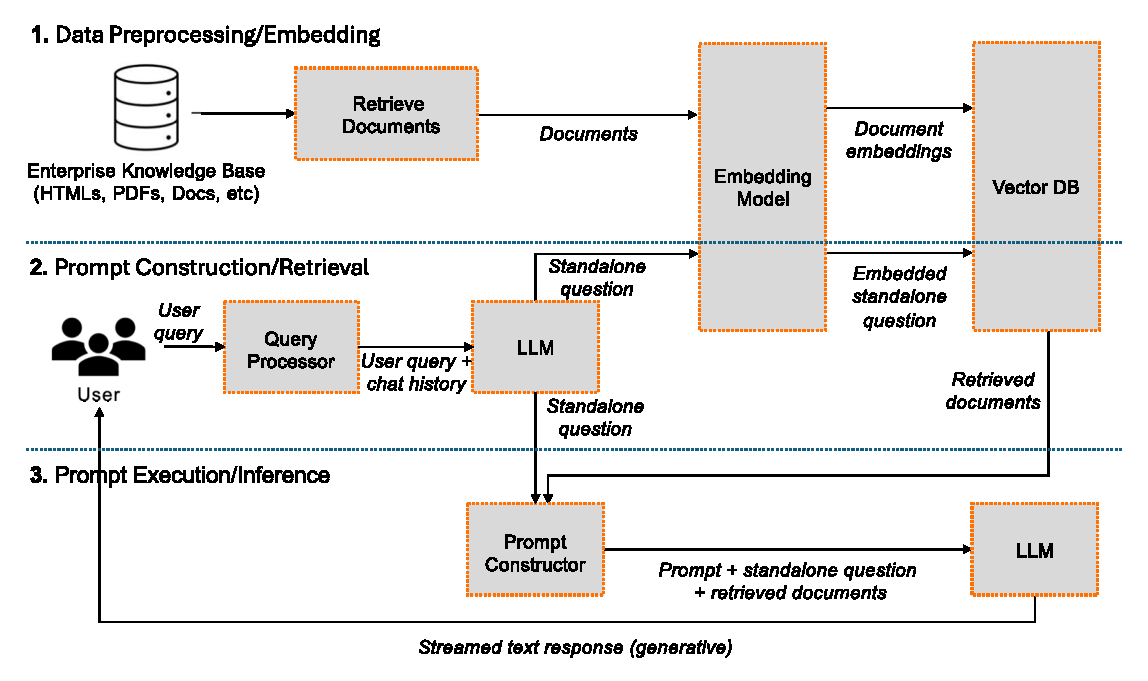
\includegraphics[width=1\textwidth]{figures/RAG.eps}    
    \caption{Overview of the RAG system architecture used in our experiments.}
    \label{fig:rag_architecture}
\end{figure}

\subsubsection{Document Processing}

Documents are processed through the following pipeline:

\begin{enumerate}[leftmargin=*]
    \item \textbf{Text Extraction:} PDF documents are parsed using specialized libraries to extract text while preserving structural information.
    
    \item \textbf{Chunking:} Documents are segmented into chunks of approximately 500 tokens with 50-token overlap to maintain context continuity.
    
    \item \textbf{Embedding:} Text chunks are encoded using the HuggingFace Instructor model~\cite{su2023instructor}, generating 768-dimensional dense vectors.
    
    \item \textbf{Indexing:} Embeddings are stored in FAISS~\cite{johnson2019faiss} for efficient similarity search.
\end{enumerate}

\subsubsection{Retrieval Configuration}

For each user query, the retrieval component:
\begin{itemize}[leftmargin=*]
    \item Encodes the query using the same embedding model
    \item Performs approximate nearest neighbor search to identify top-$k$ relevant chunks ($k=10$ in our experiments)
    \item Returns retrieved chunks as context for generation
\end{itemize}

\subsubsection{Conversational Retrieval Chain}

We employ LangChain's ConversationalRetrievalChain~\cite{langchain2024} for multi-turn interactions. The chain operates in three phases:

\begin{enumerate}[leftmargin=*]
    \item \textbf{Standalone Question Generation:} Synthesizes a context-independent question from chat history and current query
    \item \textbf{Document Retrieval:} Retrieves relevant context using the standalone question
    \item \textbf{Response Generation:} Generates the final response conditioned on retrieved context
\end{enumerate}

This architecture serves as the foundation for more complex multi-agent systems presented in Chapter~\ref{ch:agentic}, where retrieval and generation are orchestrated across specialized agents.

\subsection{Evaluation Datasets}

\subsubsection{PCI DSS Dataset}

For RAG-focused experiments, we utilize documents from the Payment Card Industry Data Security Standard (PCI DSS) version 4.0. This dataset comprises 13 PDF documents obtained from the PCI Security Standards Council, covering security requirements for organizations handling payment card data.

The domain-specific nature of PCI DSS demands accurate technical retrieval, concise synthesis of requirements, and context-aware compliance guidance.

Our evaluation queries focus on:
\begin{enumerate}[leftmargin=*]
    \item Basic definitional questions (``What's PCI DSS?'')
    \item Comparative analysis (``Changes from version 3.2.1 to 4.0'')
    \item Technical deep-dives (``New vulnerability assessment requirements'')
    \item Follow-up clarifications (``More on penetration testing'')
\end{enumerate}

\subsubsection{MS MARCO Dataset}

For broader in-context learning evaluation, we utilize a subset of the MS MARCO dataset~\cite{bajaj2016msmarco}. We curated 500 queries with well-formed answers across five categories:

\begin{table}[htbp]
\centering
\caption{MS MARCO Evaluation Dataset Composition}
\label{tab:msmarco_dataset}
\begin{tabular}{@{}lcc@{}}
\toprule
\textbf{Category} & \textbf{Queries} & \textbf{Example} \\
\midrule
LOCATION & 100 & Where is the Eiffel Tower? \\
NUMERIC & 100 & How many states in the US? \\
PERSON & 100 & Who invented the telephone? \\
DESCRIPTION & 100 & What is photosynthesis? \\
ENTITY & 100 & What is the capital of France? \\
\midrule
\textbf{Total} & \textbf{500} & \\
\bottomrule
\end{tabular}
\end{table}

\subsubsection{WebQSP Dataset}

For knowledge-base question answering (KBQA) evaluation, we utilize the WebQSP dataset~\cite{yih2016webqsp}, comprising 1,008 questions with entity-based answers from Wikidata. This dataset enables evaluation of LLM performance on structured knowledge retrieval tasks.

\subsection{Model Selection}

Table~\ref{tab:models_evaluated} summarizes the LLMs evaluated in our experiments, spanning proprietary and open-source alternatives across a range of parameter counts from 2B to 70B.

\begin{table}[htbp]
\centering
\caption{Large Language Models Evaluated}
\label{tab:models_evaluated}
\begin{tabular}{@{}llcl@{}}
\toprule
\textbf{Model} & \textbf{Organization} & \textbf{Parameters} & \textbf{Type} \\
\midrule
GPT-4 & OpenAI & Unknown & Proprietary \\
GPT-3.5-Turbo & OpenAI & Unknown & Proprietary \\
Orca-2-13b & Microsoft & 13B & Open-source \\
Orca-2-7b & Microsoft & 7B & Open-source \\
Llama-2-70b & Meta & 70B & Open-source \\
Llama-2-13b & Meta & 13B & Open-source \\
Llama-2-7b & Meta & 7B & Open-source \\
Llama-3-70b & Meta & 70B & Open-source \\
Llama-3-8b & Meta & 8B & Open-source \\
Gemma-1.1-7b & Google & 7B & Open-source \\
Gemma-1.1-2b & Google & 2B & Open-source \\
Phi-3-mini & Microsoft & 3.8B & Open-source \\
Mistral-7b & Mistral AI & 7B & Open-source \\
\bottomrule
\end{tabular}
\end{table}

\subsection{Evaluation Metrics}

\subsubsection{Generation Quality Metrics}

We employ the RAGAS framework~\cite{es2023ragas} for generation quality assessment:

\textbf{Faithfulness Score (FS):} Measures factual consistency between generated responses and retrieved context:

\begin{equation}
FS = \frac{\text{Number of contextually supported claims}}{\text{Total number of claims in response}}
\end{equation}

\textbf{Answer Relevancy (AR):} Assesses alignment between responses and user queries, computed as the cosine similarity between the original query and questions that the response would answer.

\textbf{Overall Score:} Harmonic mean of Faithfulness and Answer Relevancy:

\begin{equation}
\text{Overall} = \frac{2 \times FS \times AR}{FS + AR}
\end{equation}

\subsubsection{Inference Speed}

Measured as tokens generated per second, capturing practical deployment considerations for real-time applications.

\subsubsection{Answer Quality for In-Context Learning}

For MS MARCO evaluation, we employ:
\begin{itemize}[leftmargin=*]
    \item \textbf{ROUGE-L:} Longest common subsequence-based similarity~\cite{lin2004rouge}
    \item \textbf{BLEU-1:} Unigram precision with brevity penalty~\cite{papineni2002bleu}
\end{itemize}

\subsection{Hardware Configuration}

Experiments were conducted on multiple hardware configurations:

\begin{itemize}[leftmargin=*]
    \item \textbf{Consumer Desktop:} NVIDIA GeForce RTX 4090 (24GB VRAM)
    \item \textbf{Professional Workstation:} NVIDIA A40 (48GB VRAM)
    \item \textbf{High-Performance Server:} NVIDIA L40 (48GB VRAM)
\end{itemize}

This diversity enables evaluation of model performance across typical enterprise hardware tiers, informing the comprehensive hardware benchmarking presented in Chapter~\ref{ch:strategies}.

\section{Comparative Evaluation of LLMs for RAG}
\label{sec:rag_comparative}

\subsection{Generation Quality Results}

Figure~\ref{fig:generation_quality} presents generation quality metrics across evaluated models on the PCI DSS benchmark.

\begin{figure}[htbp]
    \centering
    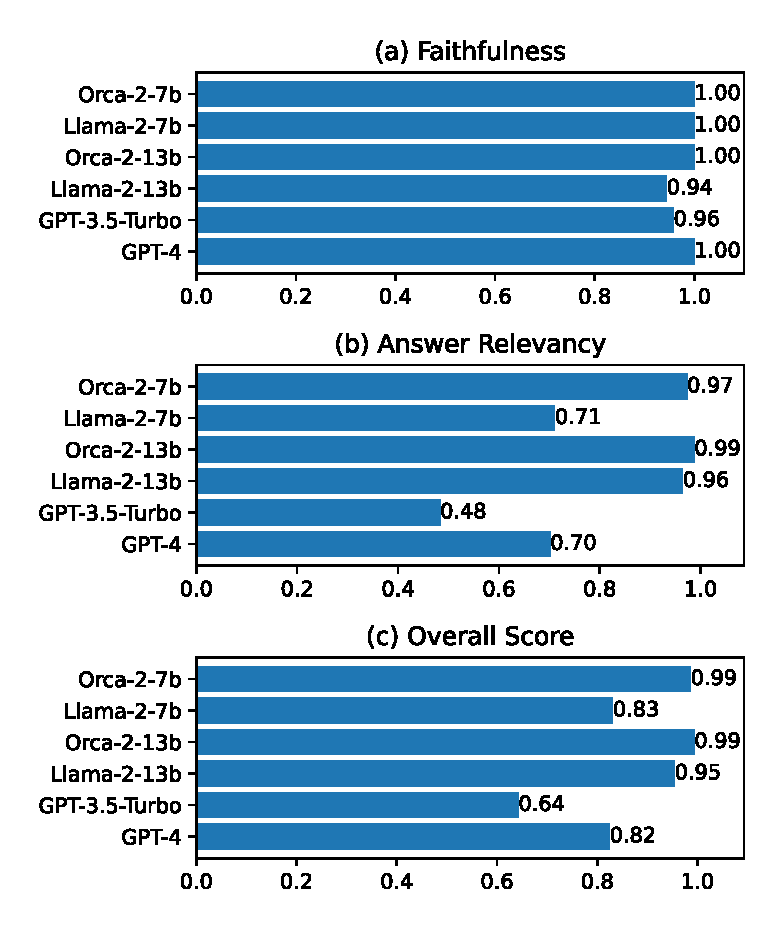
\includegraphics[width=0.9\textwidth]{figures/perf_scores.eps}
    \caption{Comparison of generation quality metrics across LLMs on PCI DSS benchmark.}
    \label{fig:generation_quality}
\end{figure}

Key observations include:

\textbf{Faithfulness:} All models except GPT-3.5-Turbo and Llama-2-13b achieved perfect faithfulness scores (100\%), indicating strong factual consistency with retrieved context. The lower scores for GPT-3.5-Turbo appear attributable to its tendency to rely on parametric knowledge rather than retrieved context.

\textbf{Answer Relevancy:} Orca-2-13b and Orca-2-7b achieved top performance, with scores approaching 99\%. This demonstrates their effectiveness in providing contextually relevant responses aligned with user queries.

\textbf{Overall Score:} Orca-2-13b achieved the highest overall score (99.3\%), followed closely by Orca-2-7b (99.2\%), indicating balanced performance across quality dimensions.

Table~\ref{tab:rag_results_summary} summarizes the quantitative results.

\begin{table}[htbp]
\centering
\caption{RAG Generation Quality Results on PCI DSS Benchmark}
\label{tab:rag_results_summary}
\begin{tabular}{@{}lccc@{}}
\toprule
\textbf{Model} & \textbf{Faithfulness (\%)} & \textbf{Answer Relevancy (\%)} & \textbf{Overall (\%)} \\
\midrule
Orca-2-13b & 100.0 & 98.7 & 99.3 \\
Orca-2-7b & 100.0 & 98.5 & 99.2 \\
GPT-4 & 100.0 & 95.2 & 97.5 \\
Llama-2-7b & 100.0 & 92.1 & 95.9 \\
GPT-3.5-Turbo & 87.3 & 89.8 & 88.5 \\
Llama-2-13b & 91.2 & 85.4 & 88.2 \\
\bottomrule
\end{tabular}
\end{table}

\subsection{Open-Source Model Competitiveness}

A central finding of our evaluation is that properly configured open-source models can match or exceed proprietary alternatives for RAG applications. Orca-2-13b achieved a 99.3\% overall RAGAS score---surpassing GPT-4 (97.5\%) while operating on consumer-grade hardware. This finding challenges the assumption that proprietary models are necessary for high-quality RAG deployment and has significant implications for enterprise cost management and data privacy.

The performance advantage of Orca-2 models appears attributable to their training methodology, which emphasizes learning from complex explanation traces rather than simply imitating larger models~\cite{mitra2023orca}. This training approach produces models that more reliably follow retrieved context rather than defaulting to parametric knowledge---a critical capability for enterprise RAG applications where accuracy must be grounded in organizational documents.

This finding---that smaller, specialized models can outperform larger general-purpose alternatives---recurs throughout this dissertation. In Chapter~\ref{ch:agentic}, we observe similar patterns where qwen2.5:32b matches GPT-4.1 performance for invoice reconciliation, and in Chapter~\ref{ch:strategies}, DeepSeek-R1:32b substantially outperforms DeepSeek-R1:70b on sentiment classification tasks.

\subsection{Inference Speed Analysis}

Figure~\ref{fig:inference_speed} presents inference speed comparisons.

\begin{figure}[htbp]
    \centering
    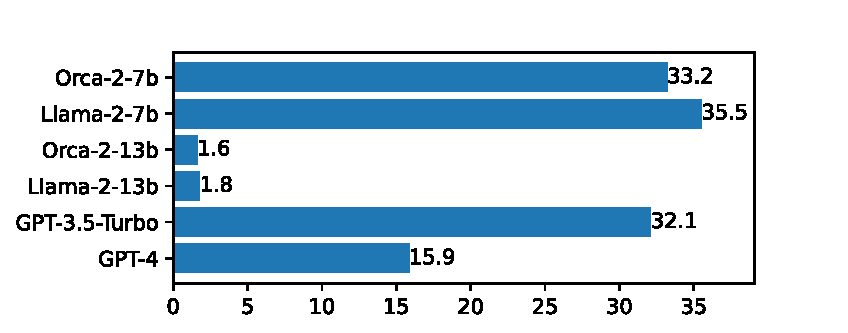
\includegraphics[width=0.9\textwidth]{figures/inference_speed.eps}
    \caption{Inference speed comparison across LLMs on consumer and professional hardware.}
    \label{fig:inference_speed}
\end{figure}

The Orca-2-7b model achieved approximately 33 tokens per second on the RTX 4090, closely matching GPT-3.5-Turbo (32 tokens/sec) and significantly outperforming GPT-4 (16 tokens/sec). This demonstrates that smaller, efficient models can provide competitive throughput on consumer-grade hardware.

Notable observations:
\begin{itemize}[leftmargin=*]
    \item 13B parameter models exhibited slower speeds due to GPU memory constraints
    \item Running Orca-2-13b on the A40 (48GB) improved speed to approximately 15 tokens/sec
    \item Hardware memory capacity significantly impacts larger model performance
\end{itemize}

\subsection{Qualitative Analysis}

Examination of generated responses revealed several patterns:

\textbf{Language Switching:} Orca-2-13b occasionally switched to Spanish after the first question while maintaining high quality scores. This indicates that RAGAS evaluation---utilizing GPT-4-Turbo---assesses quality based on semantics rather than language consistency.

\textbf{Standalone Question Generation:} Models exhibited varying quality in generating standalone questions for retrieval. Orca-2-7b sometimes produced generic questions, while other models maintained query specificity.

\textbf{Context Utilization:} GPT-3.5-Turbo and GPT-4 occasionally ignored retrieved context in favor of parametric knowledge, explaining their lower faithfulness scores in some scenarios. This behavior is particularly problematic for enterprise applications where responses must be grounded in organizational documents.

\section{The Repetition-Aware Performance Metric}
\label{sec:rag_rap}

When optimizing a RAG system, it is crucial to employ evaluation metrics that can effectively guide both system development and automated hyperparameter tuning. Standard metrics for QA or text generation (e.g., accuracy, F1, BLEU) capture how well the generated content aligns with the ground truth but fail to account for issues like redundancy or verbosity. In open-source LLMs---particularly those not rigorously RLHF-tuned for conciseness---repetitive outputs are common~\cite{fu2020repetition}. For instance, a model might repeat a sentence from the context multiple times or generate unnecessarily long sequences of non-word characters, such as repeated newlines. Such behavior not only degrades user experience but can also indirectly reduce accuracy if key information becomes obscured by repetitive content. This is particularly problematic in tasks requiring coherent and contextually relevant responses, such as conversational chatbots and---as we demonstrate in Chapter~\ref{ch:agentic}---multi-agent systems where output quality directly impacts downstream component reliability.

To address this, the \textit{repetition penalty parameter} (RPP) is employed during the sampling process to reduce redundant outputs by penalizing previously seen tokens~\cite{keskar2019ctrl}. While effective, excessive application of RPP can result in incomplete or fragmented responses, ultimately diminishing user satisfaction.

To address this issue, we introduced the \emph{Repetition-Aware Performance} (RAP) metric in our NAACL 2025 paper~\cite{huang2025rap}. That work investigates the relationship between the repetition penalty parameter (RPP) and its effect on generated text. While parameters like \textit{temperature} and \textit{top-k sampling} are typically optimized via random or grid search, these approaches are inadequate for tuning RPP because conventional metrics, such as precision and BLEU scores~\cite{papineni2002bleu}, fail to account for repetition.

To address this, we propose a metric called \textbf{R}epetition-\textbf{A}ware \textbf{P}erformance (RAP), which quantifies repetition and penalizes it in the model's performance evaluation, allowing for the tuning of RPP. 
Figure~\ref{fig:hook} illustrates tuning RPP for Llama-3-8B using the original evaluation metrics (Original) and our proposed metric. For the WebQSP dataset~\cite{yih2016webqsp}, repetition ratio (RR) is reduced by 93.1\% but the performance only drops by 3.7\%. For the MS MARCO dataset~\cite{bajaj2016msmarco}, RR drops by 73.9\% with only 3.7\% of performance drop. Tuning RPP using RAP can significantly reduce the RR with minimal performance loss. 

\begin{figure}[htbp]
    \centering
    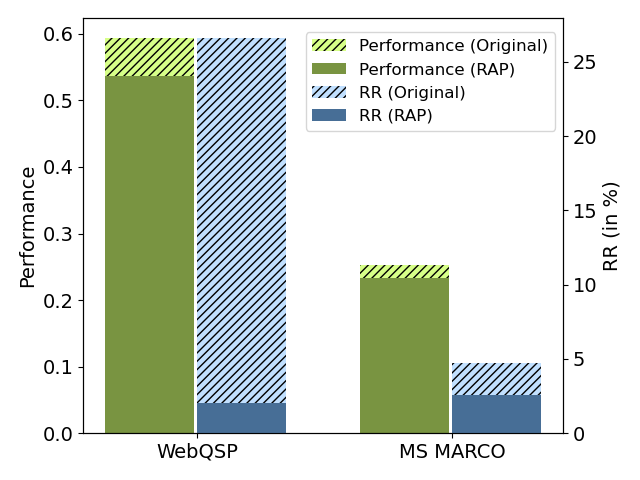
\includegraphics[width=.7\linewidth]{rap_image/chart_00_w_legend_Meta-Llama-3-8B-Instruct(RAG - Generic Prompt)_2.png}
    \caption{Best performance (F1 for WebQSP, BERT-F1 for MS MARCO) when tuning RPP using original evaluation metrics (Original) and our proposed repetition-aware performance metric (RAP). RAP helps find RPP values that minimally reduce performance while significantly lowering repetition ratio (RR). Result is from Llama-3-8B (RAG-Generic Prompt).}
    \label{fig:hook}
\end{figure}

To compute RAP, we introduce an efficient algorithm called ReDA---Repetition Detection Algorithm---designed to identify all repeating patterns, including non-word character (NWC) and text repetitions, along with their corresponding repetition lengths. Additionally, we define the repetition ratio (RR), which measures the proportion of repeated content relative to the total text length. RR is applied to penalize the model's performance using a cubic penalty formula, as detailed in Section~\ref{sec:rap_definition}. Figure~\ref{fig:overall} illustrates computing RAP with a running example. Although the accuracy is 100\%, the content contains many repeated elements, resulting in a low RAP score of 24.63\%.

\begin{figure*}[htbp]
    \centering
    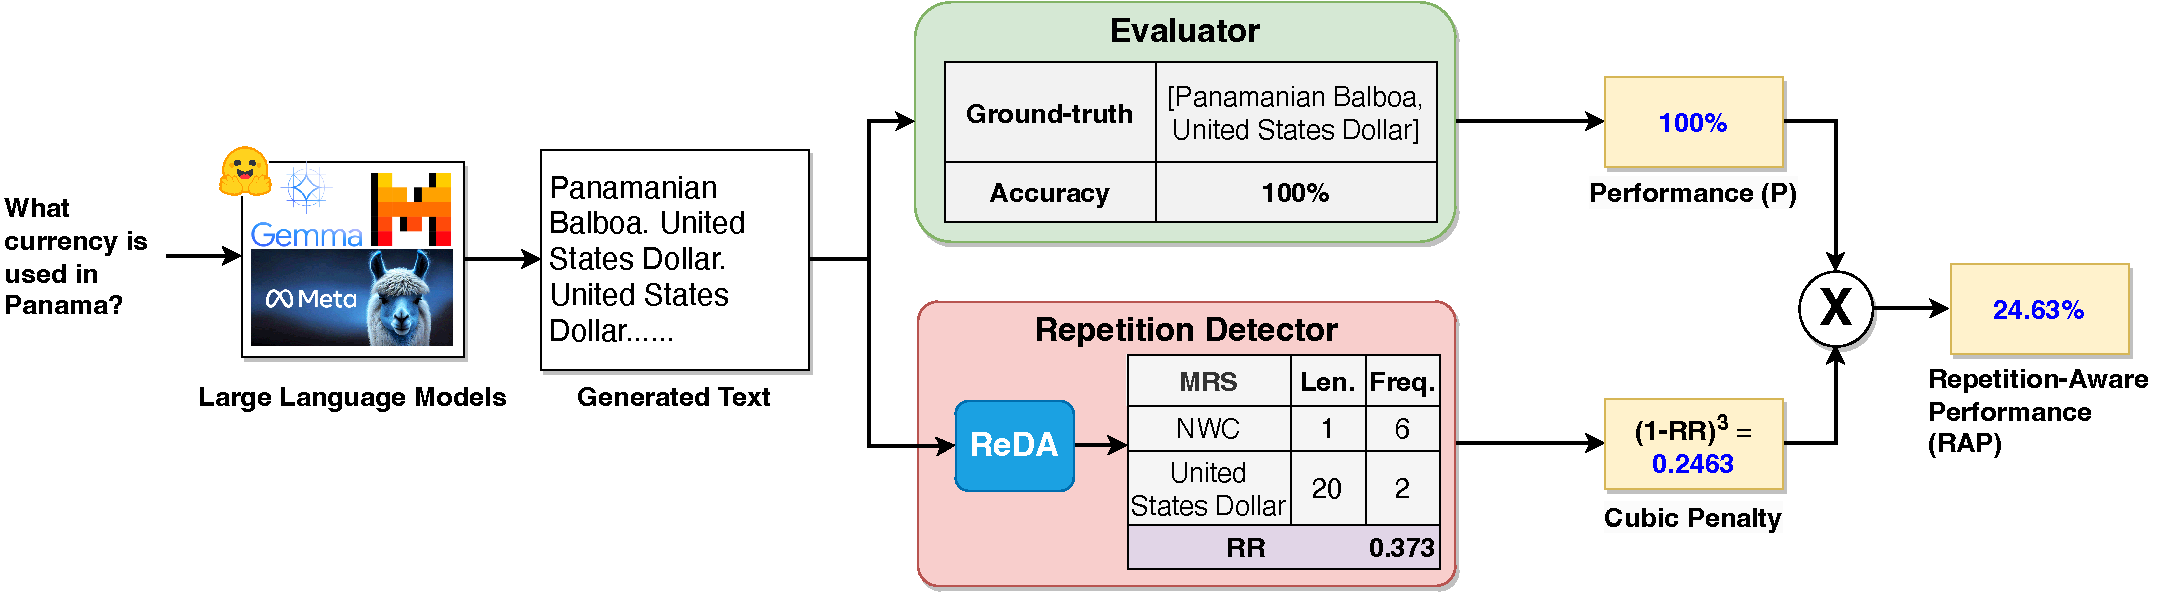
\includegraphics[width=\textwidth]{rap_image/RAPGeT_v3-v5.2.pdf}
    \caption{Overall Methodology: RAP integrates the repetition penalty in the evaluation score. In the example, the generated text contains non-word characters (NWC) repetition and text repetition. After penalization, the accuracy is reduced from 100\% to 24.63\%. ReDA stands for Repetition Detection Algorithm.}
    \label{fig:overall}
\end{figure*}

We conduct experiments on three datasets encompassing question answering (including knowledge base question answering---KBQA---and open-ended QA) and machine translation tasks.
We evaluate twelve open-source LLMs ranging from 2 to 70 billion parameters. 
We also examine the effect of repetition suppression for different prompting strategies including Retrieval-Augmented Generation (RAG)~\cite{lewis2020rag} and non-RAG, combining with generic prompt and chat template.

Our study reveals that increasing RPP typically reduces repetition but often results in performance degradation, highlighting the importance of tuning RPP. The effects of RPP differ across various models, datasets, and prompting techniques. Additionally, we find that using chat templates is effective in reducing repetition for QA tasks. Our experimental results demonstrate that RAP can effectively tune RPP, helping to identify a trade-off value that significantly reduces repetition while minimizing performance loss.
These findings offer insights into optimizing RPP for performance and repetition suppression in open-source LLMs.

\subsection{Repetition Ratio (RR)}
\label{sec:rr_definition}

First, we define the \textbf{Repetition Ratio (RR)} for a set of outputs (e.g., all answers in an evaluation set). The repetition ratio measures the portion of the generated text that is composed of repetitive content. To compute RR, repetition must be detected at both the character level (e.g., excessive whitespace or punctuation) and the word/phrase level. We employ a repetition detection algorithm (ReDA) that identifies two types of repetition:
\begin{itemize}[leftmargin=*]
    \item \textbf{Non-word Character (NWC) Repetition:} Sequences of spaces or other non-alphanumeric characters that are overly long (e.g., multiple newline characters or dashes), indicating that the model is stalling or outputting blank lines.
    \item \textbf{Textual Repetition:} Longer sequences of words that repeat. We search for any substring of length $\geq L$ (a threshold such as 5 characters) that appears at least twice in the output.
\end{itemize}

For each generated output $S$, let $R(S)$ denote the total length (in characters) of all repeated segments identified in $S$ (summing lengths from both NWC and textual repetition). Let $|S|$ be the total length of $S$. Then, the repetition ratio for a single output is defined as:
\[
r(S) = \frac{R(S)}{|S|}.
\]
For an entire set $D$ of outputs, the aggregate repetition ratio is given by:
\begin{equation}
\text{RR}_D = \frac{\sum_{S \in D} R(S)}{\sum_{S \in D} |S|}\,.\label{eq:rr_dataset}
\end{equation}
Here, $\text{RR}_D = 0$ indicates no repetition, while a value of $0.10$ indicates that 10\% of the generated text is redundant.

In practice, $R(S)$ is implemented using regular expressions to detect runs of whitespace, punctuation, and repeated substrings efficiently~\cite{huang2025rap}. Algorithm~\ref{alg:reda} provides pseudocode for the ReDA algorithm, which iteratively removes detected repetitions and sums their lengths.

\begin{algorithm}[htbp]
\caption{Repetition Detection (ReDA)~\cite{huang2025rap}}
\label{alg:reda}
\begin{algorithmic}[1]
\Require Generated text $S$
\Ensure Repetition lengths $L_{\text{NWC}}, L_{\text{text}}, L_{\text{total}}$
\State $L_{\text{NWC}} \gets 0$, $L_{\text{text}} \gets 0$
\State Use regex to find any occurrence of 5 or more non-word characters in a row in $S$
\If{matches found}
    \State Remove these sequences from $S$ and increment $L_{\text{NWC}}$ by the total number of removed characters
\EndIf
\State Use regex to find repeated textual patterns of length $\geq 5$ in $S$
\For{\textbf{each} match of a repeated substring of length $\ell$ in $S$}
    \State $L_{\text{text}} \gets L_{\text{text}} + \ell$ \Comment{Accumulate lengths of repeats}
\EndFor
\State $L_{\text{total}} \gets L_{\text{NWC}} + L_{\text{text}}$
\State \Return $(L_{\text{NWC}}, L_{\text{text}}, L_{\text{total}})$
\end{algorithmic}
\end{algorithm}

\subsection{Defining the RAP Score}
\label{sec:rap_definition}

With $\text{RR}_D$ computed, we define the RAP score for the model's outputs. Let $P$ be the base performance metric of interest (e.g., average F1 score, exact match accuracy, BERT-F1, or COMET, depending on the task). We incorporate a repetition penalty through a function $F(\text{RR}_D)$ that decreases from 1 as $\text{RR}_D$ increases. In our work, we use a cubic penalty for smoothness:
\[
F(\text{RR}) = (1 - \text{RR})^3\,.
\]
The RAP score is then defined as:
\begin{equation}
\text{RAP} = P \times F(\text{RR}_D)\,.\label{eq:rap}
\end{equation}
If the model produces no repetition ($\text{RR}_D = 0$, so $F=1$), then $\text{RAP} = P$. If there is any repetition, then $0 < F < 1$, leading to $\text{RAP} < P$, effectively lowering the performance score in proportion to the repetition. For example, if $\text{RR}_D = 0.1$ (10\% repetition), then $F(0.1) = 0.9^3 \approx 0.729$, meaning the model retains roughly 73\% of its base score under RAP. This approach incentivizes reducing repetition.

RAP is valuable in two ways:
\begin{enumerate}[leftmargin=*]
    \item It can guide hyperparameter tuning (see Section~\ref{sec:rag_opt}). For instance, when tuning the repetition penalty parameter (RPP), using only accuracy might select a configuration with higher accuracy but excessive redundancy. RAP leads to choosing an RPP that balances performance and conciseness.
    \item It allows for holistic model comparisons. In our experiments, while larger models had higher raw performance, some smaller models achieved comparable RAP scores due to reduced redundancy---an important insight for enterprise deployments.
\end{enumerate}

It is important to ensure that RAP does not excessively penalize necessary repetitions. In some contexts, repeating critical instructions---such as ``Please read carefully. Please read carefully.''---is essential for ensuring emphasis and clarity. Our ReDA algorithm is designed to detect only excessive or verbose repetitions; small amounts of repetition yield a penalty factor close to 1. In practice, we found that RAP correlates well with human judgments of answer quality when redundancy is taken into account.

\subsection{Experimental Settings}
\label{sec:rap_experiments}

\textbf{Datasets.} We conduct our experiments on three datasets: WebQSP~\cite{yih2016webqsp} and MS MARCO~\cite{bajaj2016msmarco} for question answering (QA), and MAC~\cite{huang2025translation} for Chinese-English machine translation (MT). The test sets contain 1,008, 500, and 1,133 questions, respectively. For WebQSP, we crawl relevant Wikipedia articles and retrieve the 8 most pertinent document chunks per question to form RAG prompts. We also adopt Gemini-1.0-Pro to evaluate the knowledge base QA (KBQA) task, where ground-truth answers consist of lists of entities rather than free-form text.

\paragraph{Cross-Task Validation with Machine Translation.}
While this chapter focuses primarily on RAG optimization for question answering, we include machine translation (MT) experiments to demonstrate the generalizability of the RAP metric. The repetition problem is not unique to RAG-based QA---it manifests across diverse generation tasks. Validating RAP on MT establishes its applicability as a general-purpose evaluation metric for open-source LLMs, regardless of whether retrieved context is involved. This cross-task validation strengthens confidence in RAP's utility for enterprise deployments spanning multiple use cases. The MT findings presented here lay groundwork for the comprehensive translation evaluation in Chapter~\ref{ch:strategies}, where we introduce additional metrics (Translation Completeness Ratio, Characters per Second) for deployment-oriented assessment.

\textbf{Open-Source LLMs.} This study evaluates a diverse set of open-source large language models (LLMs) for question answering (QA) and machine translation (MT) tasks. For QA, we assess nine models: Llama-2 (7B, 13B, 70B), Llama-3 (8B, 70B), Gemma-1.1 (2B, 7B), Phi-3-mini (3.8B), and Mistral-7B. For MT, we evaluate three models: Phi-3.5-mini (3.8B), Mistral-7B, and Llama-3.1-70B. Table~\ref{tab:ai_models} provides an overview of these models---including their companies, model names, Hugging Face identifiers, and the tasks on which they were evaluated. This selection spans a broad range of model sizes and architectures, representing the state of the art in open-source LLM development and commercial use.

\begin{table*}[htbp]
\caption{Overview of Large Language Models and Their Specifications by Task}
\label{tab:ai_models}
\centering
\resizebox{.85\textwidth}{!}{
\begin{tabular}{l|l|l|l}
\toprule
\textbf{Company} & \textbf{Model Name} & \textbf{Hugging Face Model ID} & \textbf{Task} \\
\midrule
\multirow{6}{*}{Meta} 
& Llama-2-7B & meta-llama/Llama-2-7b-chat & QA \\
& Llama-2-13B & meta-llama/Llama-2-13b-chat & QA \\
& Llama-2-70B & meta-llama/Llama-2-70b-chat & QA \\
& Llama-3-8B & meta-llama/Meta-Llama-3-8B-Instruct & QA \\
& Llama-3-70B & meta-llama/Meta-Llama-3-70B-Instruct & QA \\
& Llama-3.1-70B & shenzhi-wang/Llama3.1-70B-Chinese-Chat & MT \\
\midrule
\multirow{2}{*}{Microsoft} 
& Phi-3-mini & microsoft/Phi-3-mini-128k-instruct & QA \\
& Phi-3.5-mini & microsoft/Phi-3.5-mini-instruct & MT \\
\midrule
\multirow{2}{*}{Google} 
& Gemma-1.1-2B & google/gemma-1.1-2b-it & QA \\
& Gemma-1.1-7B & google/gemma-1.1-7b-it & QA \\
\midrule
\multirow{2}{*}{Mistral AI} 
& Mistral-7B-v0.2 & mistralai/Mistral-7B-Instruct-v0.2 & QA \\
& Mistral-7B-v0.3 & shenzhi-wang/Mistral-7B-v0.3-Chinese-Chat & MT \\
\bottomrule
\end{tabular}
}
\end{table*}

\textbf{Automating QA and MT Tasks with LLMs.} We developed a Python script leveraging the HuggingFace Transformers library~\cite{wolf2020transformers} to automate evaluation across all models and datasets. For QA, a repetition penalty (RP) ranging from 1.0 to 1.3 (in increments of 0.02) was applied; for MT, an RP range of 1.0 to 1.1 was used. To ensure consistency and reproducibility, the temperature was set to 0 and \texttt{top\_p} was fixed at 0.95.

\textbf{Prompt Templates.} To explore the impact of prompting strategies, we implemented three QA prompt templates: (1) \textit{RAG - Generic Prompt} (RAG-GP): a uniform template applied to all models; (2) \textit{RAG - Chat Template} (RAG-CT): LangChain's default template adapted to each LLM's chat format, preserving core content; and (3) \textit{Non-RAG}: a template simulating a single-turn conversation in the LLM's native chat format. For MT, we employed two templates: (1) \textit{MT - Generic Prompt} (MT-GP): a basic template applied uniformly; and (2) \textit{MT - Chat Template} (MT-CT): a template customized to each LLM's chat format.

The following listings describe the prompt templates used in our experiments.

\begin{lstlisting}[caption={RAG - Generic Prompt template for question answering. The placeholders \texttt{\{question\}} and \texttt{\{context\}} are filled with the question and retrieved data, respectively.},label={list:rag-generic},basicstyle=\small\ttfamily,breaklines=true,frame=single]
Use the following pieces of context to answer the question at the end. If you don't know the answer, just say that you don't know, don't try to make up an answer.
{context}
Question: {question}
Helpful Answer:
\end{lstlisting}

\begin{lstlisting}[caption={Non-RAG prompt template for question answering with Llama-3 models. The placeholder \texttt{\{question\}} is filled with the question.},label={list:non-rag},basicstyle=\small\ttfamily,breaklines=true,frame=single]
<|begin_of_text|>
<|start_header_id|>system<|end_header_id|>
You are a chatbot having a conversation with a human.
<|eot_id|>
<|start_header_id|>user<|end_header_id|>
{question}
<|eot_id|>
<|start_header_id|>assistant<|end_header_id|>
\end{lstlisting}

\begin{lstlisting}[caption={RAG - Chat Template for Llama-3 models. The placeholders \texttt{\{question\}} and \texttt{\{context\}} are filled with the question and retrieved data, respectively.},label={list:rag-chat},basicstyle=\small\ttfamily,breaklines=true,frame=single]
<|begin_of_text|>
<|start_header_id|>system<|end_header_id|>
You are a chatbot having a conversation with a human.
<|eot_id|>
<|start_header_id|>user<|end_header_id|>
Use the following pieces of context to answer the question at the end. If you don't know the answer, just say that you don't know, don't try to make up an answer.
{context}
Question: {question}
<|eot_id|>
<|start_header_id|>assistant<|end_header_id|>
\end{lstlisting}

\begin{lstlisting}[caption={Machine Translation - Generic Prompt (MT-GP) for all models. The placeholder \texttt{\{input\}} is filled with the Chinese sentence from the MAC testing set.},label={list:mt-generic},basicstyle=\small\ttfamily,breaklines=true,frame=single]
You will be given a Chinese sentence to translate. If it is an incomplete sentence, or if you are unsure about the meaning, simply copy the input text as your output. Do not output any additional sentences, such as explanations or reasoning.
Chinese: {input}
\end{lstlisting}

\begin{lstlisting}[caption={Machine Translation - Chat Template (MT-CT) for Llama-3 models. The placeholder \texttt{\{input\}} is filled with the Chinese sentence from the MAC testing set.},label={list:mt-chat},basicstyle=\small\ttfamily,breaklines=true,frame=single]
<|begin_of_text|>
<|start_header_id|>system<|end_header_id|>
You are a helpful assistant that translates Chinese to English.
<|eot_id|>
<|start_header_id|>user<|end_header_id|>
You will be given a Chinese sentence to translate. If it is an incomplete sentence, or if you are unsure about the meaning, simply copy the input text as your output. Do not output any additional sentences, such as explanations or reasoning.
Chinese: {input}
<|eot_id|>
<|start_header_id|>assistant<|end_header_id|>
\end{lstlisting}

\textbf{Evaluation Metrics.} For WebQSP, we report precision, recall, and F1 scores. For MS MARCO, we use BERTScore~\cite{zhang2020bertscore} (with the deberta-xlarge-mnli model) and report the average F1 score (\textit{BERT-F1}). For MAC, we employ the Crosslingual Optimized Metric for Evaluation of Translation (COMET)~\cite{rei2022comet}, which leverages contextual embeddings from pretrained language models to assess translation quality. In addition, we report the repetition ratio (Equation~\ref{eq:rr_dataset}) and the RAP scores (Section~\ref{sec:rap_definition}), which incorporate a penalty for repetition into the performance metrics.

\subsection{Impact of RPP on Repetition and Performance}
\label{subsec:impact_of_rpp}

\begin{figure*}[htbp]
    \centering
    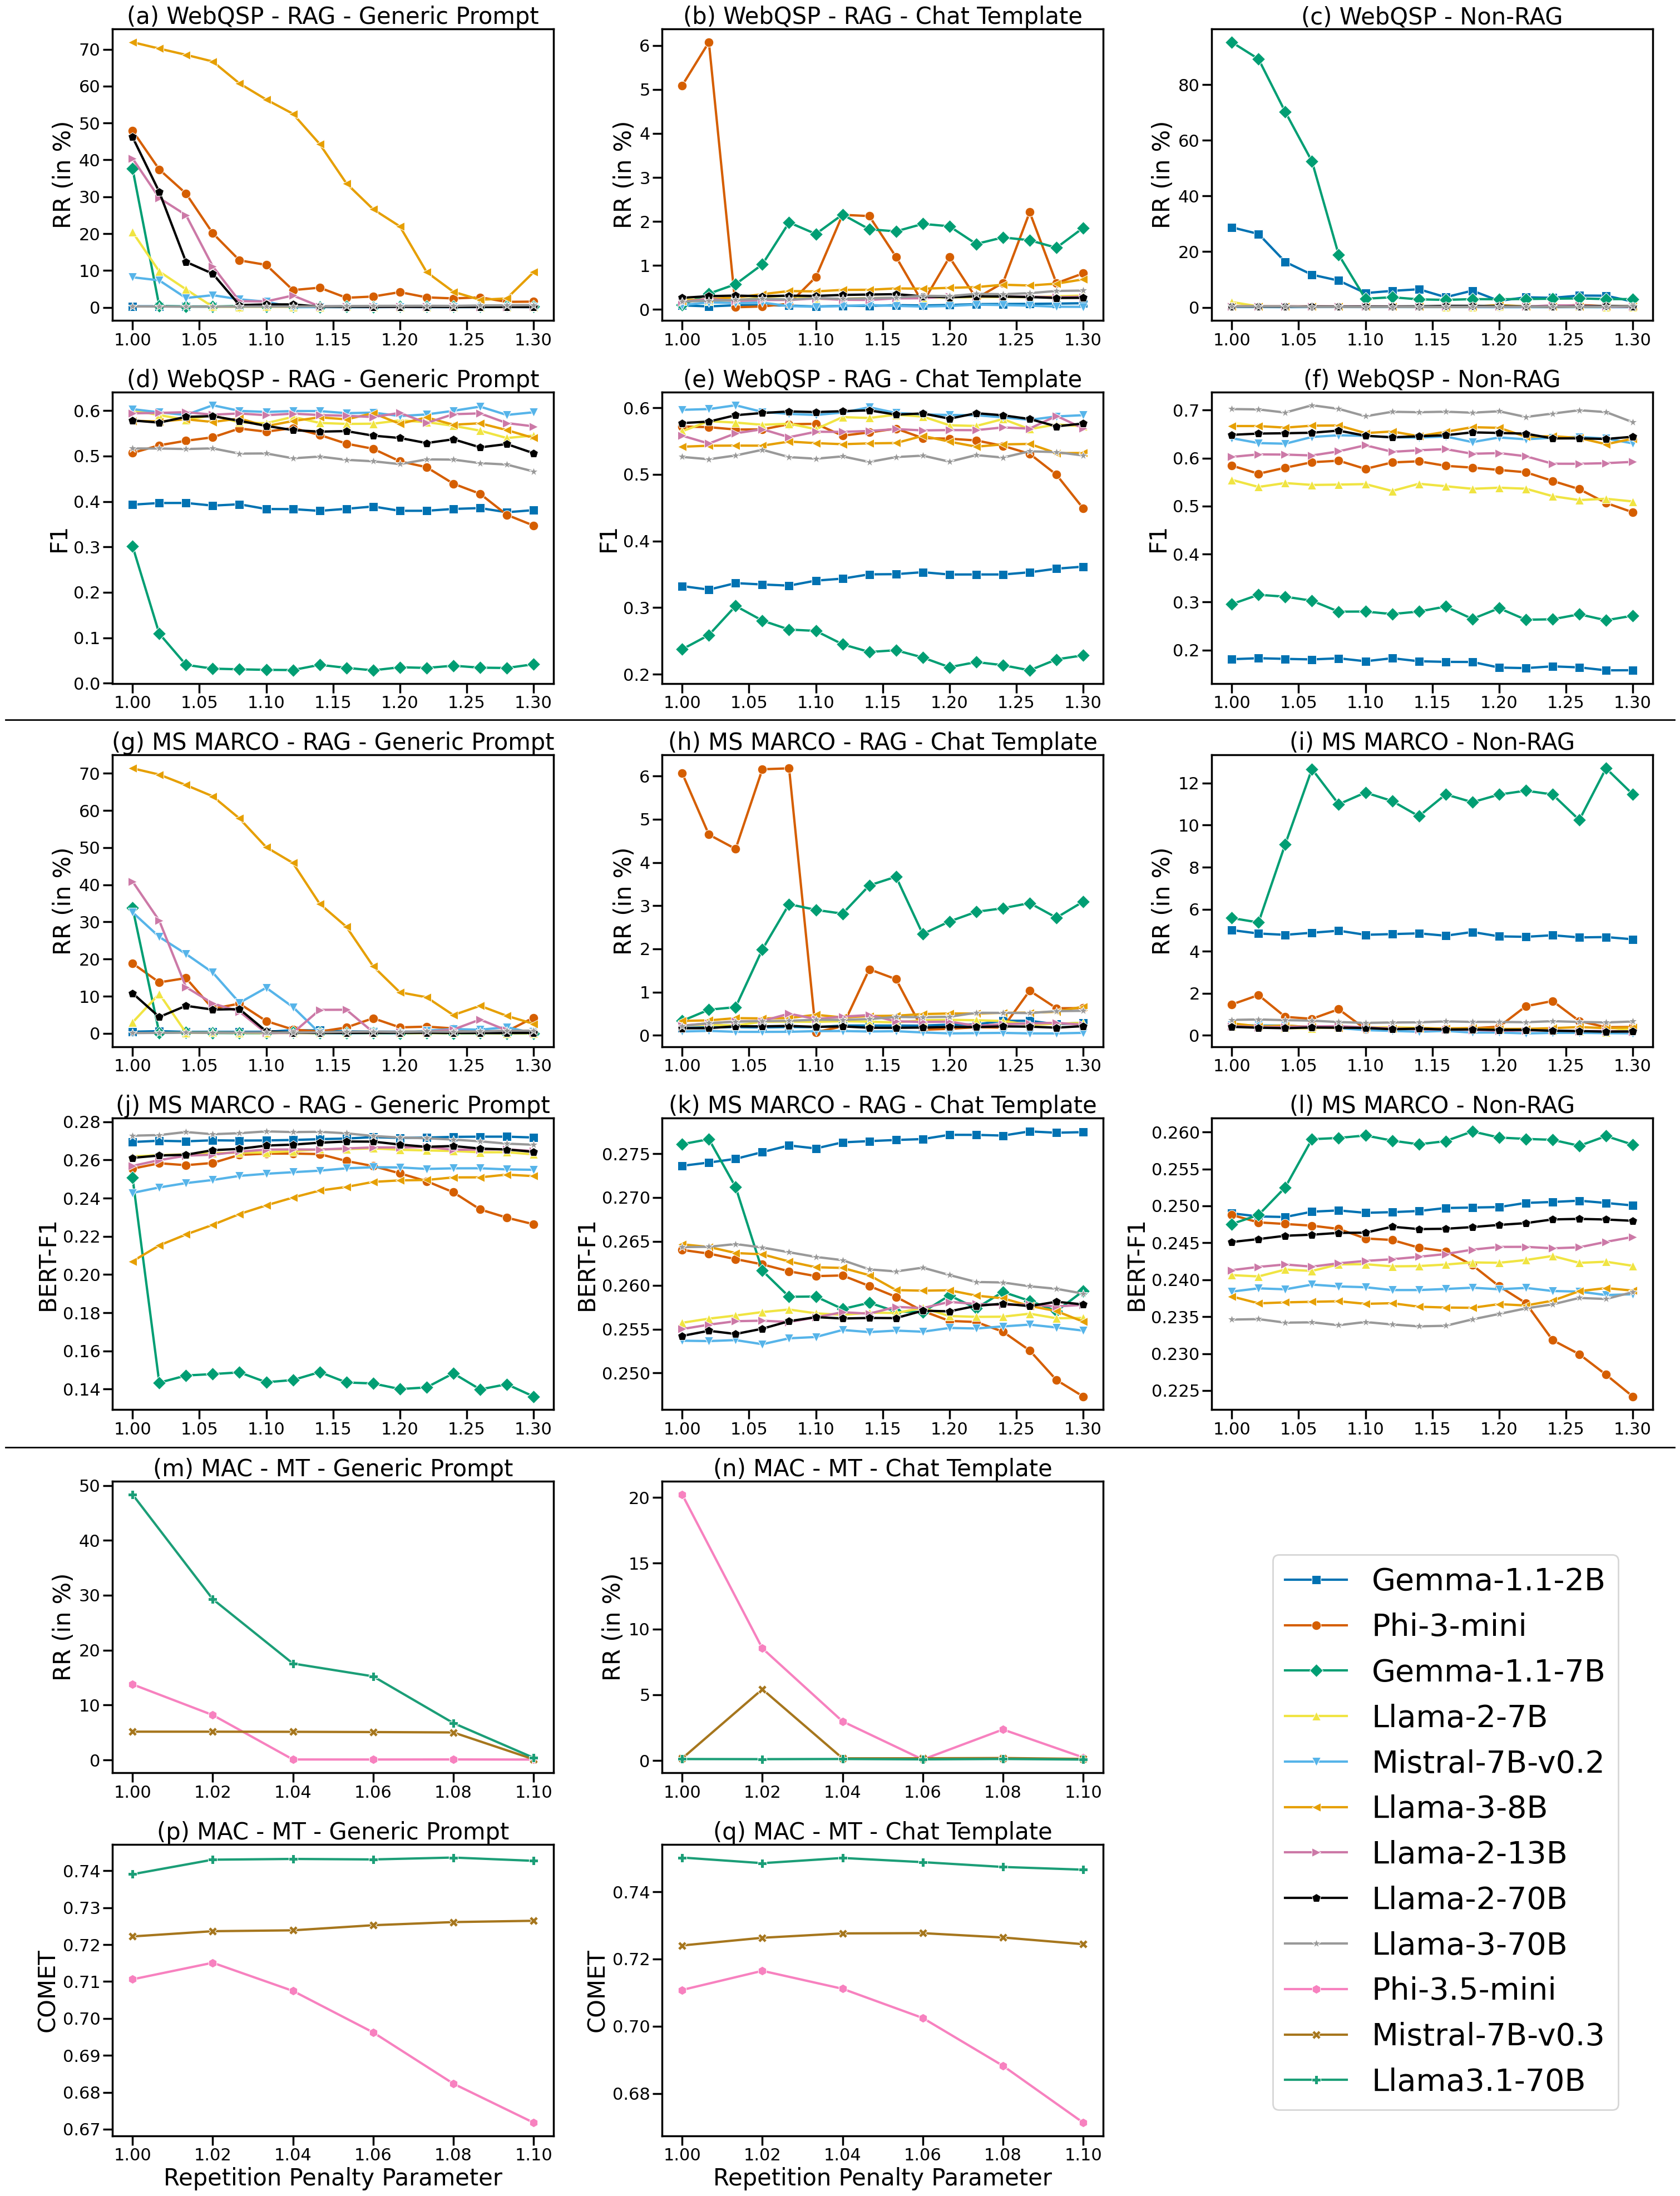
\includegraphics[width=\textwidth]{rap_image/all-metrics-across-models_v2.png}
    \caption{Illustrating the impact of RPP on the repetition ratio (RR) and performance across models, datasets, and prompting strategies.}
    \label{fig:all-metrics-across-models_v2}
\end{figure*}

Figure~\ref{fig:all-metrics-across-models_v2} shows the effect of varying RPP on the repetition and performance of different open-source LLMs across three datasets and multiple prompting strategies. The results indicate that increasing RPP generally reduces repetition; however, this often comes at the expense of performance. The trends and severity vary by model. For example, Phi-3-mini's performance on the MS MARCO dataset drops significantly when RPP exceeds 1.14, whereas Llama-3-8B improves under higher RPP settings. Thus, selecting an optimal RPP is crucial to balance repetition reduction with minimal performance loss.

The datasets also behave differently. WebQSP tends to exhibit higher baseline repetition (e.g., at RPP = 1.0) than MS MARCO, particularly when using the RAG-GP strategy. In the MAC dataset for machine translation, repetition decreases with increasing RPP, even though a smaller range is tested. Notably, for both QA datasets, the Chat Template strategy consistently produces lower RR values compared to the Generic Prompt approach, indicating its effectiveness in minimizing repetition. However, this advantage is not as pronounced in the MT task, where increasing RPP effectively reduces repetition for both prompting strategies.

\subsection{Optimizing the Trade-Off Between Performance and Repetition}
\label{sec:eval_tuning}

\begin{figure*}[htbp]
    \centering
    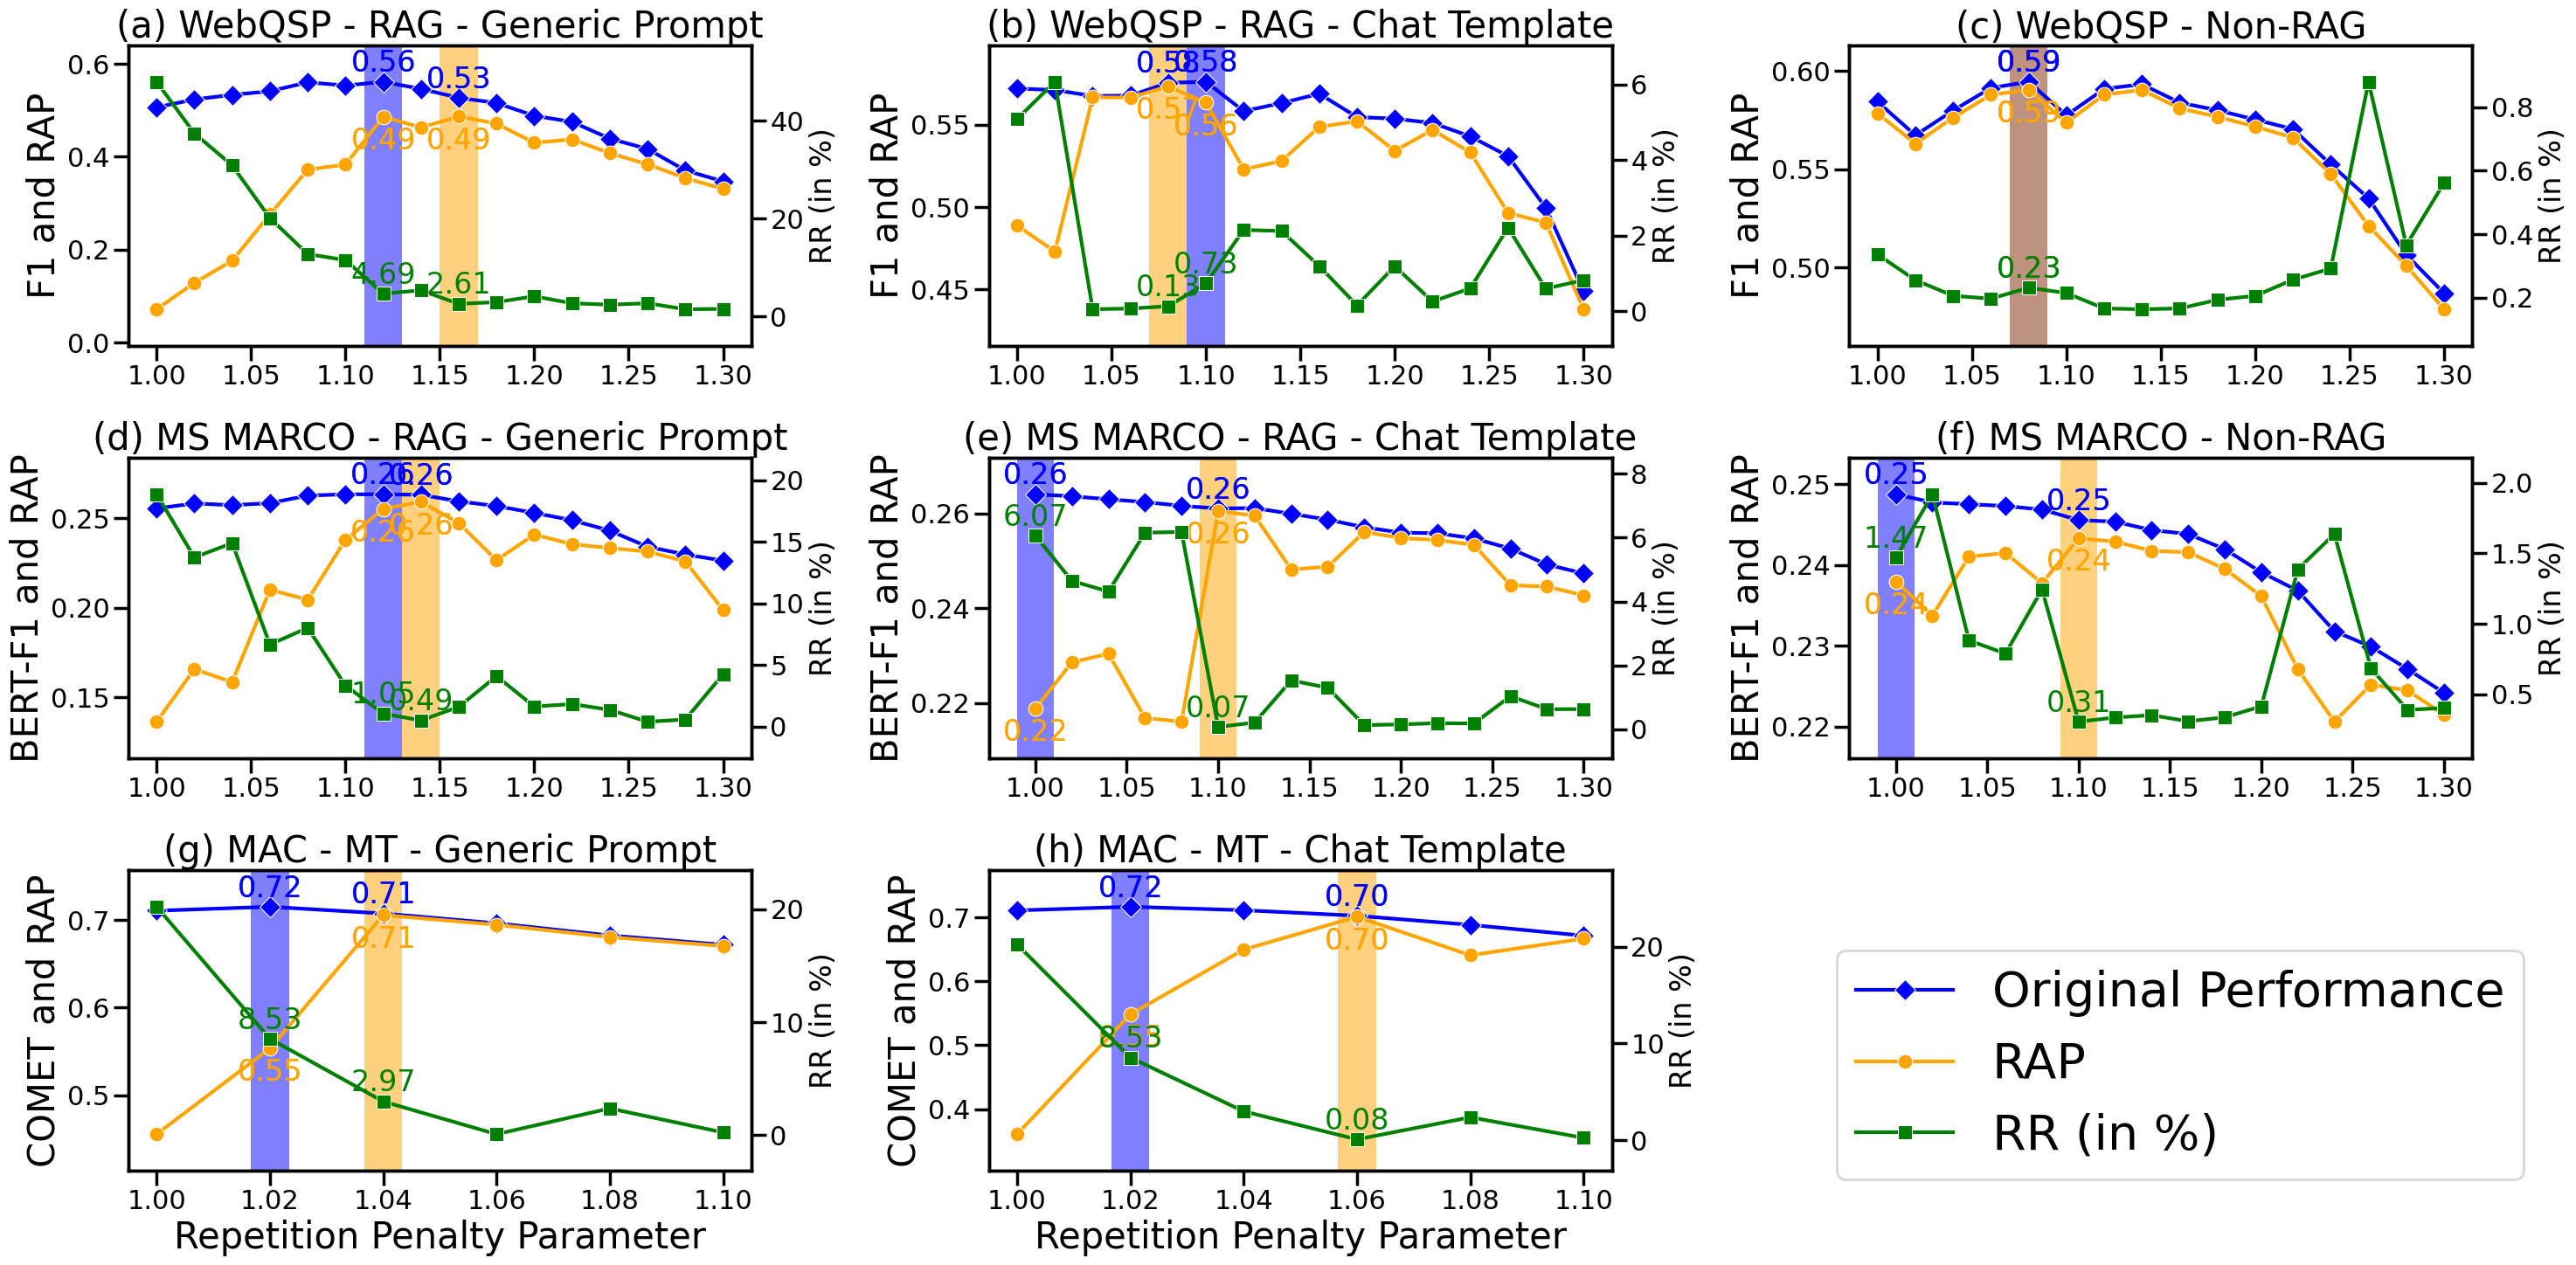
\includegraphics[width=\textwidth]{rap_image/performance_vs_repetition_v2.png}
    \caption{Original performance, repetition-aware performance (RAP), and repetition ratio (RR) for Phi-3-mini in QA (subplots (a) to (f)) and Phi-3.5-mini in MT (subplots (g) and (h)) as a function of RPP. Blue lines represent original performance (F1 for WebQSP, BERT-F1 for MS MARCO, COMET for MAC), orange lines indicate RAP scores, and green lines (right y-axis) show the RR in percentage. The blue shaded region marks the RPP for optimal original performance, the orange region highlights the best RAP, and brown indicates overlap between the two.}
    \label{fig:performance_vs_repetition_v2}
\end{figure*}

This section demonstrates the use of RAP for tuning RPP by comparing conventional performance metrics and repetition-aware performance. Figure~\ref{fig:performance_vs_repetition_v2} presents results for Phi-3-mini on WebQSP and MS MARCO, and for Phi-3.5-mini on MAC. The blue line shows the original performance, the orange line the RAP score, and the green line indicates the repetition ratio (RR). The shaded regions indicate the optimal RPP according to conventional metrics (blue) and RAP (orange); brown shading marks overlapping regions. In most cases (except Figure~\ref{fig:performance_vs_repetition_v2}c), the optimal RPP differs when tuned for original performance versus RAP. For instance, in Figure~\ref{fig:performance_vs_repetition_v2}e, tuning with BERT-F1 yields an optimal RPP of 1.0 with a performance of 0.264 and a high repetition ratio of 6.07\%. With RAP, the optimal RPP shifts to 1.1, where performance drops by only 1.1\% (to 0.261), but the repetition ratio decreases significantly (by about 98.8\%). These results highlight that tuning RPP with RAP better balances performance and repetition reduction.

\subsection{Comparing the RAP-Tuned Performance of All Models}

\begin{table}[htbp]
\centering
\caption{Comparison of model performance across different datasets, LLMs, and prompting strategies.}
\label{tab:model-performance}
\resizebox{.85\columnwidth}{!}{
\begin{tabular}{p{1.2cm}|l|ccc}
\toprule
\multicolumn{1}{l|}{\textbf{Dataset}} & \textbf{LLM} & \textbf{RAG-GP} & \textbf{RAG-CT} & \textbf{Non-RAG} \\ 
\midrule
\multirow{9}{*}{\makecell{WebQSP}} & Gemma-1.1-2B & 0.397 & 0.361 & 0.175 \\
                                   & Phi-3-mini & 0.527 & 0.575 & 0.595 \\
                                   & Gemma-1.1-7B & 0.109 & 0.302 & 0.291 \\
                                   & Mistral-7B-v0.2 & \textbf{0.609} & \textbf{0.604} & 0.648 \\
                                   & Llama-2-7B & 0.589 & 0.590 & 0.548 \\
                                   & Llama-3-8B & 0.572 & 0.558 & 0.668 \\
                                   & Llama-2-13B & 0.595 & 0.588 & 0.627 \\
                                   & Llama-2-70B & 0.577 & 0.596 & 0.657 \\
                                   & Llama-3-70B & 0.517 & 0.537 & \textbf{0.710} \\ 
\midrule
\multirow{9}{*}{\makecell{MS\\MARCO}} & Gemma-1.1-2B & 0.272 & \textbf{0.277} & \textbf{0.250} \\
                                      & Phi-3-mini & 0.263 & 0.261 & 0.246 \\
                                      & Gemma-1.1-7B & 0.149 & 0.276 & 0.249 \\
                                      & Mistral-7B-v0.2 & 0.256 & 0.256 & 0.239 \\
                                      & Llama-2-7B & 0.266 & 0.257 & 0.243 \\
                                      & Llama-3-8B & 0.252 & 0.265 & 0.239 \\
                                      & Llama-2-13B & 0.265 & 0.258 & 0.246 \\
                                      & Llama-2-70B & 0.270 & 0.258 & 0.248 \\
                                      & Llama-3-70B & \textbf{0.275} & 0.264 & 0.238 \\ 
\midrule
\multirow{4}{*}{MAC} & \textbf{LLM} & \textbf{MT-GP} & \textbf{MT-CT} &  \\ \cmidrule{2-5}
                     & Phi-3.5-mini & 0.707 & 0.702 & \\
                     & Mistral-7B-v0.3 & 0.726 & 0.728 & \\
                     & Llama3.1-70B & \textbf{0.743} & \textbf{0.750} & \\ 
\bottomrule
\end{tabular}
}
\end{table}

Table~\ref{tab:model-performance} presents the performance of various open-source LLMs after tuning RPP using RAP. On \textbf{WebQSP}, Mistral-7B leads for both RAG-GP and RAG-CT, scoring 0.609 and 0.604, respectively, while Llama-3-70B achieves the highest F1 of 0.710 in the Non-RAG condition. For \textbf{MS MARCO}, Gemma-1.1-2B excels in both RAG-CT and Non-RAG, with scores of 0.277 and 0.250, respectively, whereas Llama-3-70B attains the best score of 0.275 under RAG-GP. In the MT task (\textbf{MAC}), Llama-3.1-70B outperforms others in both the generic and chat template categories, scoring 0.743 and 0.750. These results demonstrate that larger models like Llama-3-70B and Mistral-7B generally deliver superior performance across datasets and prompting strategies, while mid-sized models like Gemma-1.1-2B can perform competitively on specific tasks. Model choice should therefore be task-dependent rather than based solely on size.

\subsection{How Severe Can Repetition Be?}

\begin{figure}[htbp]
    \centering
    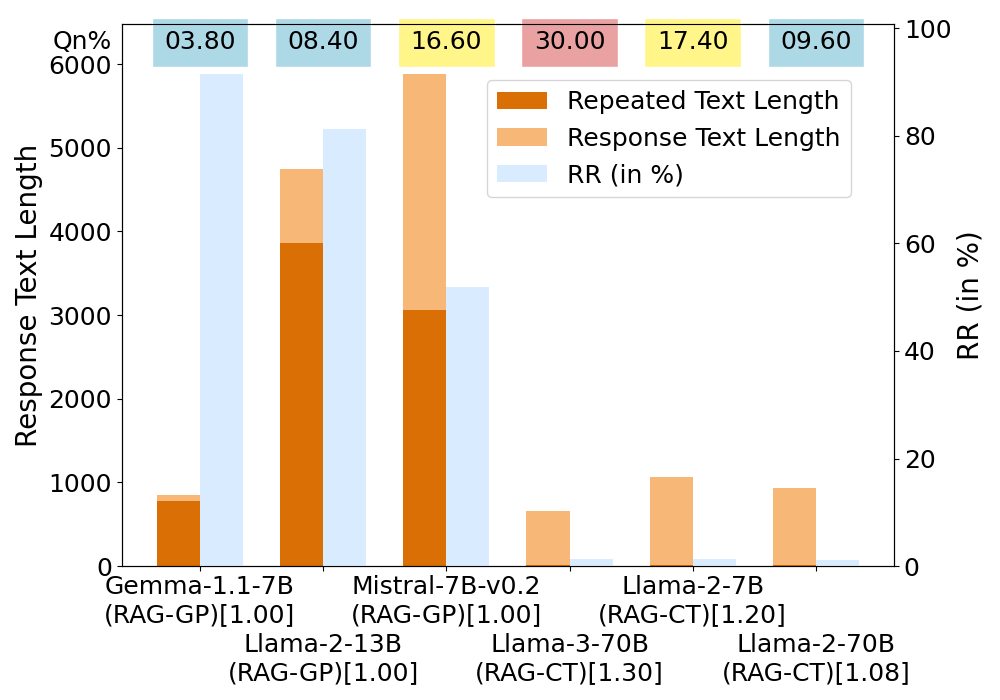
\includegraphics[width=1\linewidth]{rap_image/chart_02_mm.png}
    \caption{Severity of repetition. Colored squares above each point indicate the percentage of repetitive responses. The x-axis labels include the model, prompting method, and tuned RPP value.}
    \label{fig:msmarco_top3}
\end{figure}

In our experiments, repeated text can account for up to 97.85\% of the overall output, and up to 41.27\% of responses exhibit repetition. Figure~\ref{fig:msmarco_top3} shows the three highest and three lowest repetition ratios (RR) for the MS MARCO dataset. Colored squares above each point indicate the percentage of repeated responses (blue: below 10\%, yellow: 10--20\%, red: above 20\%). Notably, while Gemma-1.1-7B (RAG-GP) shows only 3.8\% of responses with repetition, in those cases the repeated text makes up 91.53\% of the total output length. In contrast, although 30\% of Llama-3-70B (RAG-CT)'s responses contain repetition, the repeated text comprises only 1.29\% of the overall length. For example, Llama-2-13B generated repeated content averaging around 4,000 characters.

These severity findings underscore the importance of addressing repetition not only for user experience but also for downstream system reliability. In multi-agent systems (Chapter~\ref{ch:agentic}), repetitive outputs from one agent can propagate errors through the pipeline, degrading overall workflow success rates. The RAP metric thus serves as both an evaluation tool and a quality gate for production deployments.

\subsection{Ablation Study: Effects of Different Penalty Functions}

\begin{figure}[htbp]
    \centering
    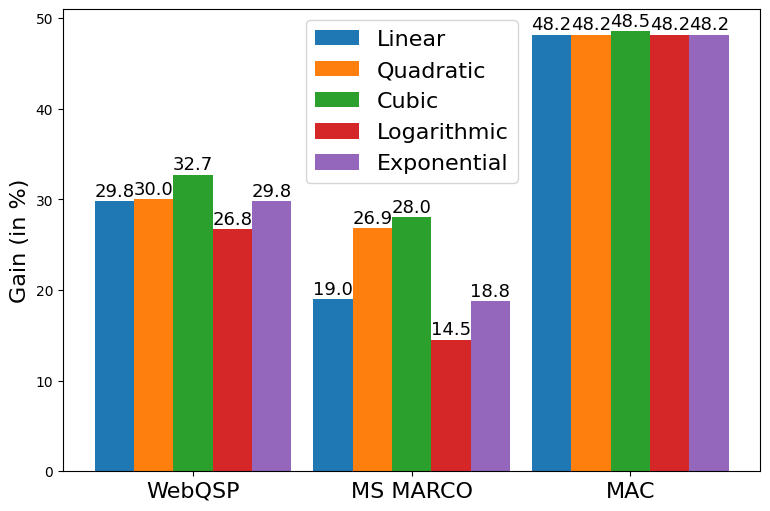
\includegraphics[width=\linewidth]{rap_image/ablation_study.png}
    \caption{Gains across different penalty functions. The \textit{Cubic} penalty consistently achieves the highest gains across all three datasets.}
    \label{fig:ablation_study}
\end{figure}

We present an ablation study to evaluate the impact of different penalty functions $F(\text{RR})$ on the RAP metric (Equation~\ref{eq:rap}). We consider five options:
\begin{itemize}[leftmargin=*]
    \item \textit{Linear}: $F(\text{RR})=1-\text{RR}$,
    \item \textit{Quadratic}: $F(\text{RR})=(1-\text{RR})^2$,
    \item \textit{Cubic}: $F(\text{RR})=(1-\text{RR})^3$,
    \item \textit{Logarithmic}: $F(\text{RR})=\log_{2}(2-\text{RR})$,
    \item \textit{Exponential}: $F(\text{RR})=e^{-\text{RR}}$.
\end{itemize}

We compare the \textit{Gain} achieved with each penalty formula. For a given model, \textit{Gain} is defined as the difference between the reduction in repetition and the performance drop when tuning the repetition penalty parameter (RPP) using original performance metrics versus RAP. In other words, it reflects the relative decrease in repetition compared to the loss in performance; a higher \textit{Gain} indicates a more favorable trade-off.

Figure~\ref{fig:ablation_study} shows the average \textit{Gain} scores for each penalty function across the three datasets, computed by averaging the gains from all models and prompting strategies. The results indicate that the \textit{Cubic} penalty consistently yields the highest gains (32.7\% for WebQSP, 28.0\% for MS MARCO, and 48.5\% for MAC), offering the best balance between reducing repetition and maintaining performance. These findings recommend the \textit{Cubic} penalty for the RAP metric across diverse datasets and tasks.

\subsection{Summary of RAP Findings}

This research tackles the challenge of reducing repeated content generation while preserving overall performance in open-source LLMs. We propose the repetition-aware performance metric, RAP, which quantifies and integrates repetition penalty into model evaluation. Conventional metrics often overlook repetition, making it difficult to tune the repetition penalty parameter (RPP). In contrast, RAP enables effective tuning of RPP and can be easily applied to other repetition methods as well.

We evaluated RAP on twelve open-source LLMs using three datasets across QA and MT tasks, with different prompting strategies. Results show that higher RPP values generally reduce repetition but can significantly impact performance. This phenomenon emphasizes the need for tuning RPP. 
The experiments also demonstrate the capability of using RAP for identifying the RPP value that efficiently reduces repetition while minimizing performance loss.
We also highlight the severity of the repetition issues in the generated content, calling for greater attention from the research community on this matter.
Our experiments offer valuable insights into managing repetition in open-source LLMs, including a recommendation to use Chat Templates for RAG prompting.

The RAP methodology---combining detection, quantification, and penalty-based optimization---exemplifies the evaluation framework philosophy that permeates this dissertation. Just as RAP integrates output quality into traditional performance metrics, the Agentic Success Rate (Chapter~\ref{ch:agentic}) integrates pipeline reliability into task completion metrics, and the Reasoning Intensity metric (Chapter~\ref{ch:strategies}) integrates computational efficiency into accuracy assessment. This pattern of multi-dimensional evaluation addresses the fundamental insight that single-metric optimization yields systems that perform well on benchmarks but poorly in production.

\section{Evaluation-Guided Hyperparameter Search}
\label{sec:rag_opt}

Building on our prior work---including our NAACL 2025 paper on the RAP metric---we propose an evaluation-guided hyperparameter search loop for optimizing Retrieval-Augmented Generation (RAG) systems. The workflow is detailed in Algorithm~\ref{alg:hyperparameter_search}.

\begin{algorithm}[htbp]
\caption{Hyperparameter Search for RAG Optimization}
\label{alg:hyperparameter_search}
\begin{algorithmic}[1]
\Require Validation set $Q$ of queries (with ground-truth answers), initial retriever and LLM, and search space $\Lambda$ for hyperparameters (e.g., retrieval and generation settings).
\Ensure Optimal hyperparameter setting $\lambda^*$.
\For{each candidate setting $\lambda \in \Lambda$ (or using an intelligent search strategy)}
    \State Configure the retriever/LLM with $\lambda$ (e.g., set $k$, $\tau$, RPP, etc.)
    \State Generate answers $\hat{Y} = \{\hat{y}_q : q \in Q\}$ using the RAG pipeline
    \State Evaluate $\hat{Y}$ against ground truth $Y$ to obtain a performance score $P(\hat{Y}, Y)$ (e.g., average accuracy or F1)
    \State Compute repetition or other penalties $R(\hat{Y})$ (e.g., repetition ratio)
    \State Compute the overall metric $M(\hat{Y})$, which combines performance and penalties (e.g., the RAP score as in Equation~\ref{eq:rap})
    \State Record $(\lambda, M(\hat{Y}))$
\EndFor
\State \textbf{return} $\lambda^* = \arg\max_{\lambda} M(\hat{Y}_\lambda)$
\end{algorithmic}
\end{algorithm}

In this procedure, the search space $\Lambda$ may be explored exhaustively or using an intelligent algorithm. The metric $M$ can be defined as the standard performance metric $P$ if accuracy is the only concern, but it is often augmented to incorporate aspects such as brevity or non-repetition. Our proposed RAP metric (see Section~\ref{sec:rap_definition}) is one such example. By using RAP as the optimization target, configurations that yield correct yet non-repetitive outputs are inherently favored.

In our work, this approach is used to tune the repetition penalty parameter (RPP). Traditional grid search using only accuracy would not differentiate between two configurations with similar accuracy but differing levels of verbosity. By contrast, an augmented metric like RAP can prioritize configurations with lower redundancy. We also verify that the final chosen $\lambda^*$ is robust, using a separate test set or cross-validation.

It is important to note that hyperparameter choices may interact. For example, extensive fine-tuning of the LLM may alter its sensitivity to decoding parameters, and a stronger retriever (providing higher quality documents) may permit a lower repetition penalty. Thus, hyperparameter optimization is an ongoing process that evolves with model development.

In conclusion, the RAP metric offers a nuanced evaluation of RAG systems, particularly when optimizing open-source LLMs prone to repetition. By integrating RAP into our development cycle, we ensure that our optimized RAG system retrieves and generates correct information in a succinct and user-friendly manner. Future work may extend RAP to include additional factors (e.g., factuality or coherence), but as a first step, it significantly enhances our ability to mitigate a common failure mode in open-source LLM generation.

\section{Practical Deployment Guidelines}
\label{sec:rag_guidelines}

Based on our comprehensive evaluation, we synthesize the following guidelines for enterprise RAG deployment:

\textbf{Model Selection.} Open-source models such as Orca-2 and Mistral-7B can achieve generation quality competitive with proprietary alternatives while offering significant advantages in deployment flexibility, cost, and data privacy. Orca-2-13b achieved 99.3\% overall RAGAS score, surpassing GPT-4 (97.5\%) while operating on consumer-grade hardware. For RAG applications requiring high faithfulness, models specifically trained to follow retrieved context (rather than relying on parametric knowledge) should be prioritized.

\textbf{Hardware Planning.} Model size should be matched to available hardware:
\begin{itemize}[leftmargin=*]
    \item 7B-parameter models perform efficiently on consumer GPUs (RTX 4090, 24GB VRAM), achieving approximately 33 tokens/second
    \item 13B+ models benefit substantially from professional-grade hardware (A40, L40 with 48GB VRAM) or cloud deployment
    \item Memory capacity is the primary constraint for larger models; insufficient VRAM leads to significant performance degradation
\end{itemize}
These hardware findings inform the comprehensive edge deployment evaluation in Chapter~\ref{ch:strategies}, where we extend benchmarking across six hardware platforms.

\textbf{Repetition Management.} The repetition penalty parameter (RPP) should be systematically tuned using RAP rather than default values:
\begin{itemize}[leftmargin=*]
    \item RAP-guided tuning achieves up to 93.1\% repetition reduction with only 3.7\% performance degradation
    \item The cubic penalty function $F(\text{RR}) = (1-\text{RR})^3$ provides optimal balance across datasets
    \item Chat templates consistently reduce repetition compared to generic prompts in RAG configurations
    \item Optimal RPP varies substantially across models and datasets---Phi-3-mini degrades sharply above RPP 1.14, while Llama-3-8B improves
\end{itemize}

\textbf{Evaluation Strategy.} Employ multi-dimensional evaluation combining faithfulness, relevance, and repetition metrics. Single-metric optimization may yield configurations that perform well on benchmarks but poorly in practice. The RAP framework demonstrates this principle: optimizing for accuracy alone selects configurations with high redundancy, while RAP-guided optimization achieves comparable accuracy with dramatically reduced repetition.

\textbf{Prompt Engineering.} Prompt template selection significantly impacts both retrieval quality and generation coherence:
\begin{itemize}[leftmargin=*]
    \item Chat templates reduce repetition and improve context utilization
    \item Model-specific templates (respecting each model's expected format) outperform generic prompts
    \item Standalone question generation quality affects retrieval relevance---models producing generic questions may retrieve suboptimal context
\end{itemize}

\section{Summary}

This chapter presented a comprehensive framework for optimizing Retrieval-Augmented Generation (RAG) systems built on open-source Large Language Models. Drawing from three accepted publications, we addressed the critical challenges of model selection, evaluation methodology, and generation quality that enterprises face when deploying RAG solutions.

Our comparative evaluation of LLMs on the PCI DSS benchmark revealed that smaller, efficient models such as Orca-2-13b can achieve generation quality competitive with---or exceeding---proprietary alternatives like GPT-4, while maintaining practical inference speeds on consumer-grade hardware. Specifically, Orca-2-13b achieved a 99.3\% overall RAGAS score with perfect faithfulness, demonstrating that model size alone does not determine RAG effectiveness. This finding---that architecture and training methodology matter more than scale---recurs throughout this dissertation and informs model selection strategies in subsequent chapters.

Central to our contribution is the Repetition-Aware Performance (RAP) metric, which addresses a pervasive yet overlooked problem in open-source LLM outputs: excessive repetition. Through systematic evaluation of twelve models across question answering and machine translation tasks, we demonstrated that repeated content can comprise over 90\% of generated text in severe cases, with up to 41\% of responses exhibiting redundancy. The RAP metric integrates a cubic penalty function that enables principled tuning of the repetition penalty parameter (RPP), achieving up to 93.1\% reduction in repetition with minimal performance degradation (typically under 4\%). Cross-task validation on machine translation confirmed RAP's generalizability beyond RAG-specific applications.

Our experimental analysis yielded several practical insights for enterprise deployment. Chat templates significantly reduce repetition compared to generic prompts in RAG configurations, providing a simple yet effective mitigation strategy. The optimal RPP varies substantially across models and datasets, underscoring the importance of systematic hyperparameter tuning rather than default settings. Additionally, hardware memory capacity critically impacts performance for larger models, with the RTX 4090 supporting efficient inference for 7B-parameter models while 13B models benefit substantially from professional-grade GPUs like the A40.

The evaluation-guided hyperparameter search procedure presented in this chapter operationalizes these findings, using RAP as the optimization target to identify configurations that balance factual accuracy, relevance, and output conciseness. This holistic approach ensures that optimized RAG systems not only retrieve and generate correct information but deliver it in a manner suitable for enterprise applications where user experience and response clarity are paramount.

The methodological contributions of this chapter---particularly the philosophy of multi-dimensional evaluation that integrates quality considerations beyond accuracy---establish foundations for subsequent chapters. Chapter~\ref{ch:agentic} extends this approach to multi-agent systems with the Agentic Success Rate (ASR) and Evaluation Completion Rate (ECR@1), while Chapter~\ref{ch:strategies} applies similar principles through Reasoning Intensity (RI) and domain-specific metrics for translation and predictive analytics.
\chapter{Agentic AI for Workflow Automation}
\label{ch:agentic}

\section{Introduction and Motivation}
\label{sec:agentic_intro}

Agentic AI extends LLM capabilities beyond single-turn interactions to autonomous, goal-directed behavior. Unlike traditional AI systems with narrowly defined tasks and explicit instructions, agentic AI dynamically reconfigures its strategies based on feedback, uncertainty, and evolving objectives. This makes it particularly valuable for automating complex business workflows that traditionally require human judgment and coordination.

This chapter addresses the second research question (RQ2): \textit{How can multi-agent LLM systems be designed and evaluated for reliable, scalable enterprise automation?} The research presented here builds upon the evaluation methodology established in Chapter~\ref{ch:rag}---particularly the philosophy of multi-dimensional evaluation that integrates quality considerations beyond accuracy---and extends it to the unique challenges of multi-agent coordination. The findings inform deployment strategies examined in Chapter~\ref{ch:strategies}, where reasoning configuration and hardware selection interact to determine system effectiveness.

This chapter presents the design and evaluation of autonomous, LLM-driven multi-agent systems for enterprise workflow automation, synthesizing findings from six peer-reviewed publications:

\begin{enumerate}[leftmargin=*]
    \item \textbf{Invoice Reconciliation System}~\cite{huang2025invoice}: Edge-deployed LLMs in multi-agent systems for SME automation (ICDSAAI 2025)
    \item \textbf{Tool Invocation Reliability Framework}~\cite{huang2026when}: Diagnostic framework for multi-agent systems introducing the 12-category error taxonomy, validated on invoice reconciliation (ICAIBD 2026, submitted)
    \item \textbf{LLM-as-Judge Framework}~\cite{huang2026judge}: Scalable test coverage evaluation with novel Evaluation Completion Rate (ECR@1) metric for operational reliability (AAAI 2026 Workshops, accepted)
    \item \textbf{Automated Acceptance Test Generation}~\cite{huang2026open}: Cooperative multi-agent system for Gherkin test generation using AutoGen Swarm, evaluated using the LLM-as-Judge framework (PAKDD 2026 Workshops, submitted)
    \item \textbf{Hierarchical Multi-Agent System for Payments}~\cite{huang2026hmasp}: End-to-end agentic payment processing with modular architecture (PAKDD 2026, submitted)
    \item \textbf{EdgeAgent Annotation Pipeline}~\cite{huang2026edgeagent}: Semi-automatic data labeling with edge-deployed LLMs, introducing the Agentic Success Rate (ASR) metric for fine-grained reliability evaluation (PAKDD 2026, submitted)
\end{enumerate}

The chapter is organized to highlight methodological progressions: Sections~\ref{sec:invoice_reconciliation}--\ref{sec:diagnostic_framework} present invoice reconciliation and its evolution into a comprehensive diagnostic framework with the 12-category error taxonomy; Sections~\ref{sec:llm_judge}--\ref{sec:cmas4g2} demonstrate how LLM-as-Judge enables automated acceptance test generation; and Sections~\ref{sec:hmasp}--\ref{sec:edgeagent} extend these methodologies to payments and annotation domains.

A key contribution of this chapter is the introduction of two novel metrics that complement the Repetition-Aware Performance (RAP) metric from Chapter~\ref{ch:rag}: the \textbf{Agentic Success Rate (ASR)}, introduced in Section~\ref{sec:edgeagent}, which provides fine-grained evaluation of tool-calling precision in multi-step workflows, and the \textbf{Evaluation Completion Rate (ECR@1)}, which measures first-attempt success rates in automated evaluation systems---both addressing critical gaps in agentic AI evaluation methodology. Together with the 12-category error taxonomy, these metrics enable systematic diagnosis of failure modes impossible with traditional binary success/failure evaluation.

\section{Foundations of Agentic AI}
\label{sec:agentic_foundations}

\subsection{Distinguishing Characteristics}

Agentic AI systems are characterized by several key capabilities that distinguish them from traditional AI applications:

\begin{itemize}[leftmargin=*]
    \item \textbf{Tool Use:} Ability to interact with external tools, APIs, databases, and services
    \item \textbf{Planning:} Decomposing complex goals into executable sub-tasks
    \item \textbf{Memory:} Maintaining state across interactions for long-term objectives
    \item \textbf{Reflection:} Self-evaluation and strategy adjustment based on outcomes
    \item \textbf{Collaboration:} Coordinating with other agents and human operators
\end{itemize}

These capabilities introduce complexity beyond single-turn generation tasks. While Chapter~\ref{ch:rag} addressed optimization challenges for RAG systems involving retrieval and generation, agentic systems must orchestrate multiple tools across multiple steps, with errors in early stages cascading through subsequent operations.

\subsection{Challenges in Enterprise Deployment}

Implementing multi-agent AI systems in enterprise settings presents several challenges~\cite{chawla2024agentic}:

\begin{enumerate}[leftmargin=*]
    \item \textbf{Coordination Complexity:} Managing multiple LLM-powered agents is computationally intensive, raising concerns about latency and resource utilization
    
    \item \textbf{Cost Management:} Costs escalate significantly when relying on proprietary cloud-based LLMs or high-performance infrastructure
    
    \item \textbf{Data Privacy:} Enterprise requirements often necessitate edge deployment, introducing technical complexities
    
    \item \textbf{Reliability:} Agent failures may stem from poor system design rather than model limitations---recent research demonstrates that LLM-based multi-agent system failures often originate from architectural decisions rather than model quality
    
    \item \textbf{Framework Maturity:} Lack of mature orchestration frameworks complicates inter-agent communication
\end{enumerate}

These challenges motivate the systematic evaluation methodology developed in this chapter, where we distinguish between orchestration failures (addressable through better prompting and architecture) and fundamental model limitations (requiring larger models or different approaches).

%% =============================================================================
%% PART 1: Invoice Reconciliation → Diagnostic Framework (Papers 1-2)
%% =============================================================================

\section{Multi-Agent Architecture for Invoice Reconciliation}
\label{sec:invoice_reconciliation}

This section presents the first of two related studies on invoice reconciliation. The initial system~\cite{huang2025invoice} establishes the multi-agent architecture and demonstrates feasibility, while Section~\ref{sec:diagnostic_framework} extends this work with a comprehensive diagnostic framework~\cite{huang2026when} introducing the 12-category error taxonomy for systematic failure characterization.

\subsection{Problem Context}

Invoice reconciliation is a critical yet labor-intensive process for businesses, particularly small and medium-sized enterprises (SMEs). The process involves matching incoming payments to outstanding invoices, cross-verifying databases, emails, and transaction documents, updating associated records and status fields, and handling exceptions and discrepancies.

Traditional automation approaches frequently fall short in handling unstructured data and accommodating complex business rules. Our multi-agent system addresses these challenges through specialized, coordinated LLM agents deployed on edge devices, ensuring data privacy while maintaining high accuracy.

\subsection{System Architecture}

Figure~\ref{fig:invoice_architecture} presents the overall architecture. The system comprises three specialized agents operating sequentially:

\begin{figure}[htbp]
    \centering
    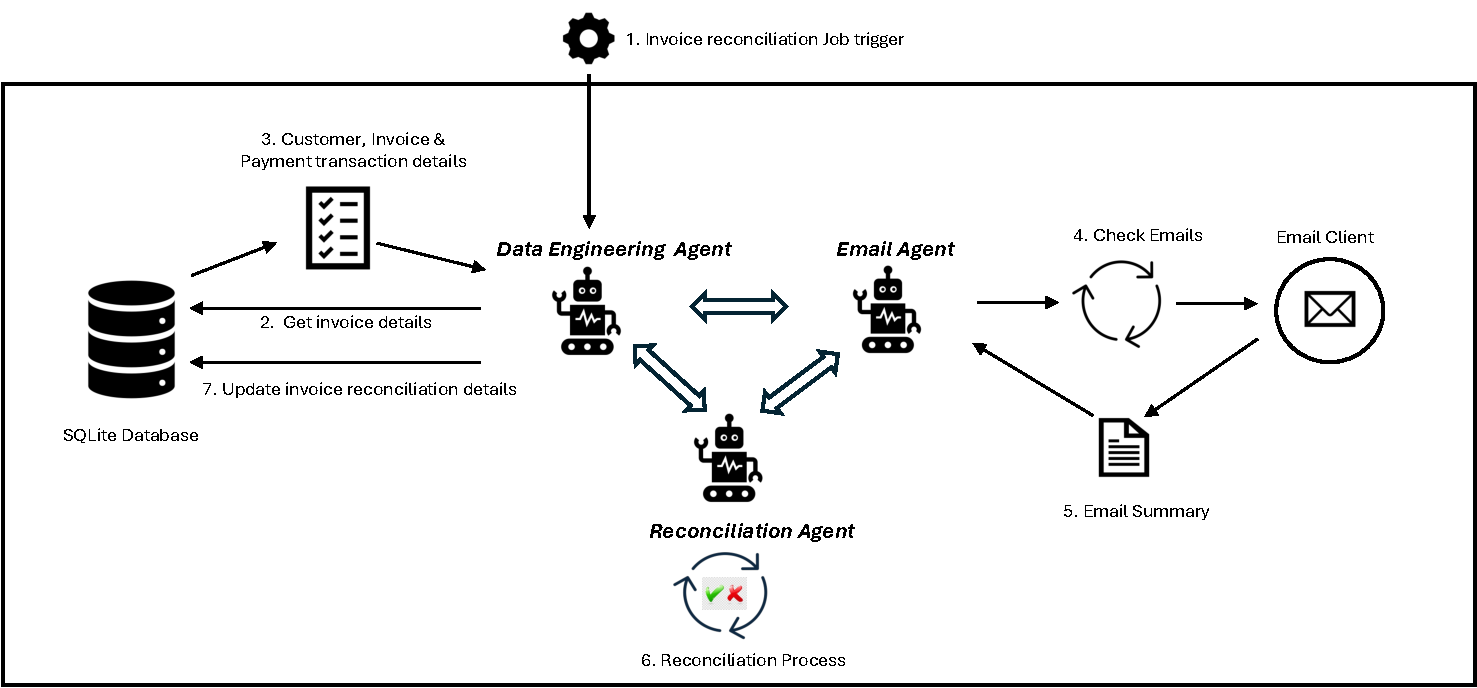
\includegraphics[width=1\textwidth]{images/invoice-rec.pdf}
    \caption{End-to-end workflow of the multi-agent architecture-based invoice reconciliation system.}
    \label{fig:invoice_architecture}
\end{figure}

\subsubsection{Data Engineering Agent}

The Data Engineering Agent serves as an intelligent interface between natural language requests and database operations, utilizing SQLite as an in-memory database for efficient business invoicing data management. Key capabilities include:

\begin{itemize}[leftmargin=*]
    \item Translating natural language queries into SQL commands
    \item Performing schema validation and query verification
    \item Executing queries against SQLite databases
    \item Converting results back to natural language summaries
\end{itemize}

The agent's architecture incorporates two primary tools: an SQL query builder and an SQL query executor, both enhanced by few-shot prompting techniques. These prompts provide essential schema information and example queries, significantly improving the accuracy and reliability of database interactions.

\subsubsection{Email Agent}

The Email Agent processes client communications and attachments through a systematic workflow:

\begin{enumerate}[leftmargin=*]
    \item Establishes live connection with email client via API
    \item Scans inbox for recent emails from customers with ``Unpaid'' status
    \item Checks for attachments and processes them using vision-based OCR
    \item Generates structured summaries of email content and extracted invoice details
\end{enumerate}

Unlike proprietary models that integrate vision capabilities, open-source models such as Functionary V3.1 and Qwen2.5 excel in function calling but lack native vision capabilities. To address this limitation, we supplemented these models with Llama3.2-Vision-11B for robust image processing functionality.

\subsubsection{Reconciliation Agent}

The Reconciliation Agent integrates outputs from other agents and performs the core matching logic:

\begin{itemize}[leftmargin=*]
    \item Combines structured data from Data Engineering and Email Agents
    \item Applies business rules for payment-invoice matching
    \item Updates database records with reconciliation results
    \item Generates status reports and exception notifications
\end{itemize}

\subsection{LangGraph-Based Orchestration}

The system is implemented using the LangGraph framework~\cite{langchain2024langgraph}, which provides graph-based architecture enabling flexible workflows, dynamic execution paths based on intermediate results, modular agent definitions for maintainability, and state management for multi-step processes.

\subsection{Experimental Setup}

\subsubsection{Hardware Configurations}

Testing was conducted on two hardware systems representing typical SME environments:

\begin{enumerate}[leftmargin=*]
    \item \textbf{RTX A6000 Desktop:} Ubuntu via WSL, 48GB VRAM, approximately \$10,000 USD
    \item \textbf{RTX 4090 Laptop:} Ubuntu via WSL, 16GB VRAM, approximately \$5,000 USD
\end{enumerate}

Due to memory constraints, only smaller models (qwen2.5:7b, functionary-small, llama3.2-vision:11b) were evaluated on the RTX 4090, while all open-source models were tested on the RTX A6000. This hardware diversity informs the comprehensive deployment evaluation in Chapter~\ref{ch:strategies}, where we extend benchmarking across six platforms.

\subsubsection{Model Selection}

Table~\ref{tab:agentic_models} lists evaluated models.

\begin{table}[htbp]
\centering
\caption{Models Evaluated for Multi-Agent Invoice Reconciliation}
\label{tab:agentic_models}
\begin{tabular}{@{}llcc@{}}
\toprule
\textbf{Model} & \textbf{Type} & \textbf{Parameters} & \textbf{Hardware} \\
\midrule
GPT-4o & Proprietary (API) & Unknown & Cloud \\
GPT-4o-mini & Proprietary (API) & Unknown & Cloud \\
Qwen2.5-72B & Open-source & 72B & RTX A6000 \\
Qwen2.5-32B & Open-source & 32B & RTX A6000 \\
Qwen2.5-7B & Open-source & 7B & Both \\
Functionary-medium & Open-source & 70B & RTX A6000 \\
Functionary-small & Open-source & 8B & Both \\
Llama3.2-vision:11B & Open-source & 11B & RTX A6000 \\
\bottomrule
\end{tabular}
\end{table}

\subsubsection{Evaluation Metrics}

\begin{itemize}[leftmargin=*]
    \item \textbf{Success Rate:} Proportion of correctly completed reconciliation tasks
    \item \textbf{Mean Execution Time:} Average time per reconciliation workflow
    \item \textbf{Energy per Task:} Joules consumed per completed task
    \item \textbf{Performance-to-Power Ratio:} Success rate normalized by energy consumption
\end{itemize}

\subsection{Results}

Table~\ref{tab:invoice_results} presents comprehensive evaluation results.

\begin{table}[htbp]
\centering
\caption{Invoice Reconciliation Performance Across Models and Platforms}
\label{tab:invoice_results}
\begin{tabular}{@{}llccc@{}}
\toprule
\textbf{Model} & \textbf{Platform} & \textbf{SUCCESS} & \textbf{NO INVOICE} & \textbf{ERROR} \\
\midrule
GPT-4o (API) & Cloud & 93.13\% & -- & -- \\
GPT-4o-mini (API) & Cloud & 97.68\% & -- & -- \\
qwen2.5:7b & RTX 4090 & 865 & 2 & 123 \\
qwen2.5:7b & RTX A6000 & 850 & 4 & 136 \\
functionary-small & RTX 4090 & 879 & 101 & 10 \\
functionary-small & RTX A6000 & 876 & 108 & 6 \\
qwen2.5:32b & RTX A6000 & \textbf{989} & 0 & 1 \\
functionary-medium & RTX A6000 & 932 & 47 & 11 \\
qwen2.5:72b & RTX A6000 & 985 & 1 & 4 \\
\bottomrule
\end{tabular}
\end{table}

Key findings:

\begin{enumerate}[leftmargin=*]
    \item \textbf{Open-source superiority:} Qwen2.5-32B achieved 99.9\% success rate (989/990), outperforming all proprietary alternatives including GPT-4o-mini (97.68\%). This finding parallels the Orca-2 results from Chapter~\ref{ch:rag}, where smaller open-source models outperformed GPT-4 on RAG tasks, reinforcing the theme that architecture and training methodology matter more than parameter count or proprietary status.
    
    \item \textbf{Execution time parity:} Edge-deployed Qwen2.5-32B execution times were comparable to cloud APIs, making it a superior candidate due to combined accuracy and speed advantages
    
    \item \textbf{Resource efficiency:} Functionary-small achieved optimal performance-to-power ratio, consuming only 523J per task on RTX 4090 while maintaining 88.78\% success rate
    
    \item \textbf{Energy trade-offs:} Larger models consume substantially more energy (19,394J for qwen2.5:72b vs 523J for functionary-small) with diminishing accuracy returns
    
    \item \textbf{Platform variations:} RTX 4090 achieved higher success rates for qwen2.5:7b and functionary-small compared to RTX A6000, underscoring its suitability for edge applications
\end{enumerate}

\subsection{Error Analysis}

Workflow outputs were categorized into three groups:

\textbf{SUCCESS:} Correctly located, identified, and processed invoice data. The workflow performed as expected, handling data extraction and reconciliation seamlessly.

\textbf{NO INVOICE:} Workflow failures due to OCR task failures (LLM hallucinations extracting non-existent information from images) or reconciliation task failures (LLM misinterpreting natural language queries and generating invalid SQL queries).

\textbf{ERROR:} Complete task failures from fundamental context misunderstanding, where the LLM completely misinterpreted workflow requirements.

Error trends across model families revealed that functionary models recorded higher NO INVOICE cases, indicating potential limitations in handling certain data reconciliation scenarios. Conversely, qwen2.5 family models exhibited greater ERROR occurrences, suggesting challenges in interpreting task context accurately.

While this initial study demonstrated the feasibility of edge-deployed multi-agent systems for invoice reconciliation, the coarse-grained error categories (SUCCESS, NO INVOICE, ERROR) limited our ability to diagnose specific failure modes. This motivated the development of the comprehensive diagnostic framework presented in the following section.

%% =============================================================================
%% Section: Diagnostic Framework - Building on Invoice Reconciliation
%% =============================================================================

\section{When Agents Fail to Act: Diagnostic Framework for Tool Invocation Reliability}
\label{sec:diagnostic_framework}

Building upon the invoice reconciliation system presented in Section~\ref{sec:invoice_reconciliation}, this section introduces a comprehensive diagnostic framework~\cite{huang2026when} that addresses a critical limitation of the initial study: the inability to systematically diagnose \textit{where} and \textit{why} workflows fail. Traditional binary success/failure metrics obscure critical diagnostic information, limiting opportunities for targeted improvements.

This diagnostic approach parallels the philosophy underlying the RAP metric from Chapter~\ref{ch:rag}: just as RAP integrates repetition quality into performance evaluation to enable principled hyperparameter tuning, our error taxonomy integrates failure mode characterization into system evaluation to enable principled architecture decisions.

\subsection{Motivation and Gap Analysis}

Current evaluation approaches for multi-agent LLM systems predominantly report aggregate task success rates~\cite{hendrycks2021measuring,zheng2024judging}, obscuring underlying failure causes. While recent work by Kokane et al.~\cite{kokane2024spectool} demonstrates the value of granular error taxonomies for single-agent tool use, these frameworks remain insufficient for multi-agent contexts where failures cascade through coordination protocols.

Consider the invoice reconciliation pipeline from Section~\ref{sec:invoice_reconciliation}: a model might correctly invoke the OCR tool but fail to initiate the subsequent database update, resulting in pipeline failure. Binary metrics would score this as complete failure, obscuring that the model successfully executed partial workflow steps---a fundamentally different (and more easily addressable) problem than complete workflow incomprehension.

This diagnostic gap has significant practical implications:
\begin{itemize}[leftmargin=*]
    \item \textbf{Model selection:} Organizations cannot determine whether failures stem from model capacity limitations or prompt design issues
    \item \textbf{System improvement:} Without granular failure characterization, developers cannot prioritize optimization efforts
    \item \textbf{Deployment decisions:} Binary metrics provide insufficient information for evidence-based deployment planning across hardware configurations
\end{itemize}

\subsection{Diagnostic Framework Overview}

Our diagnostic framework provides systematic methodology for evaluating procedural reliability in multi-agent LLM systems through two core components:

\begin{enumerate}[leftmargin=*]
    \item \textbf{12-Category Error Taxonomy:} Comprehensive failure characterization spanning tool initialization, parameter handling, execution, and result interpretation
    \item \textbf{Hardware-Performance Characterization:} Systematic evaluation across deployment configurations for deployment guidance
\end{enumerate}

The framework is designed for broad applicability across multi-agent scenarios while maintaining diagnostic precision through domain-specific instantiation. We validate this approach using the invoice reconciliation system from Section~\ref{sec:invoice_reconciliation}, demonstrating how the framework transforms coarse error categories into actionable diagnostics.

\subsection{12-Category Error Taxonomy}

For comprehensive failure characterization in multi-agent coordination scenarios, we develop a systematic error taxonomy. The taxonomy combines four error types with three tool categories, yielding twelve distinct failure modes.

\paragraph{Error Type Categories.}

\begin{itemize}[leftmargin=*]
    \item \textbf{Not Initialized:} Agent fails to properly invoke tool due to malformed calls, incorrect tool names, or invalid parameter structures
    \item \textbf{Args Mismatch:} Tool invocation succeeds but contains incorrect or invalid arguments leading to tool-specific failures
    \item \textbf{Error:} Tool executes with valid parameters but returns runtime errors or exceptions
    \item \textbf{Result Mismatch:} Tool execution succeeds but produces outputs that cause downstream task failure
\end{itemize}

\paragraph{Tool Categories.} For invoice reconciliation workflows, we define three tool categories representing common primitives in structured business automation:
\begin{itemize}[leftmargin=*]
    \item \textbf{OCR Tool:} Multi-modal document processing for receipt and invoice image analysis
    \item \textbf{DB Query Tool:} Database query operations for invoice lookup and verification
    \item \textbf{DB Update Tool:} Database modification operations for status updates
\end{itemize}

\paragraph{Complete Taxonomy.} The cross-product produces twelve diagnostic categories:

\begin{enumerate}[leftmargin=*]
    \item \texttt{OCR\_TOOL\_NOT\_INITIALIZED}: Failure to invoke OCR tool
    \item \texttt{OCR\_TOOL\_ARGS\_MISMATCH}: OCR tool called with invalid arguments
    \item \texttt{OCR\_TOOL\_ERROR}: OCR tool execution returns runtime errors
    \item \texttt{OCR\_TOOL\_RESULT\_MISMATCH}: OCR output causes downstream failures
    \item \texttt{DB\_QUERY\_TOOL\_NOT\_INITIALIZED}: Failure to invoke database query tool
    \item \texttt{DB\_QUERY\_TOOL\_ARGS\_MISMATCH}: Query tool called with invalid arguments
    \item \texttt{DB\_QUERY\_TOOL\_ERROR}: Query execution returns runtime errors
    \item \texttt{DB\_QUERY\_TOOL\_RESULT\_MISMATCH}: Query results cause downstream failures
    \item \texttt{DB\_UPDATE\_TOOL\_NOT\_INITIALIZED}: Failure to invoke database update tool
    \item \texttt{DB\_UPDATE\_TOOL\_ARGS\_MISMATCH}: Update tool called with invalid arguments
    \item \texttt{DB\_UPDATE\_TOOL\_ERROR}: Update execution returns runtime errors
    \item \texttt{DB\_UPDATE\_TOOL\_RESULT\_MISMATCH}: Update results cause downstream failures
\end{enumerate}

This taxonomy enables systematic identification of reliability bottlenecks and provides actionable diagnostic information for system improvement beyond aggregate success metrics.

\subsection{Experimental Methodology}

\subsubsection{Enhanced Multi-Agent Architecture}

We validate the diagnostic framework using the invoice reconciliation architecture from Section~\ref{sec:invoice_reconciliation}, enhanced with detailed instrumentation for failure diagnosis. Each agent is augmented with logging mechanisms to capture initialization failures, parameter mismatches, and execution errors at each tool invocation.

\subsubsection{Expanded Model Selection}

To establish comprehensive reliability benchmarks across the performance spectrum, we expand evaluation to include:

\begin{itemize}[leftmargin=*]
    \item \textbf{Closed-Source Models:} OpenAI's GPT-4 series (gpt-4o, gpt-4o-mini, gpt-4.1-nano, gpt-4.1-mini, gpt-4.1) and Anthropic's Claude models (3.5 Sonnet, 3.7 Sonnet) serve as reference baselines representing state-of-the-art proprietary systems
    \item \textbf{Open-Weight Models:} The Qwen2.5 series (3B, 7B, 14B, 32B, 72B) and Functionary V3.1 (8B, 70B) provide systematic coverage across model scales, with local deployment ensuring data sovereignty
\end{itemize}

All open-weight models were executed locally using Ollama v0.6.8 with 4-bit quantization (Q4\_K\_M format) to simulate realistic edge deployment constraints.

\subsubsection{Extended Hardware Infrastructure}

We extend testing to three representative edge platforms:

\begin{itemize}[leftmargin=*]
    \item \textbf{NVIDIA RTX A6000 Ada GPU:} High-end workstation (48GB VRAM, Ubuntu 24.04, \textasciitilde\$10K)
    \item \textbf{NVIDIA GeForce RTX 4090 Laptop GPU:} Mobile workstation (16GB VRAM, Ubuntu 24.04 via WSL, \textasciitilde\$5K)
    \item \textbf{Apple M3 Max:} Consumer-grade ARM platform (96GB unified memory, macOS 15.4.1, \textasciitilde\$4K)
\end{itemize}

\subsubsection{Evaluation Dataset and Protocol}

We employ standardized evaluation using a synthetic dataset of 1,980 test instances balanced between vision-enabled (990) and text-only (990) tasks. All experiments employ deterministic execution (temperature=0, fixed prompts), eliminating sampling variance and ensuring reproducible diagnostic assessment.

\subsection{Results and Analysis}

\subsubsection{Performance and Reliability Trade-offs}

Table~\ref{tab:asr_overall_performance} summarizes overall performance metrics across all evaluated LLM configurations.

\begin{table}[htbp]
\centering
\caption{Overall Invoice Reconciliation Performance Across LLM Configurations. SR = Success Rate. All metrics based on 1,980 test instances.}
\label{tab:asr_overall_performance}
\begin{tabular}{@{}llccc@{}}
\toprule
\textbf{Model} & \textbf{Platform} & \textbf{SR (\%)} & \textbf{Time (s)} & \textbf{Steps} \\
\midrule
\multicolumn{5}{l}{\textit{Closed-source models}} \\
gpt-4o-mini & OpenAI & 99.3 & 7.6 $\pm$ 1.6 & 8.6 $\pm$ 1.2 \\
gpt-4o & OpenAI & 98.8 & 12.4 $\pm$ 13.2 & 8.5 $\pm$ 0.6 \\
gpt-4.1-nano & OpenAI & 85.7 & 8.6 $\pm$ 12.3 & 18.5 $\pm$ 18.6 \\
gpt-4.1-mini & OpenAI & 99.5 & 8.6 $\pm$ 2.7 & 9.6 $\pm$ 1.9 \\
gpt-4.1 & OpenAI & \textbf{100.0} & 8.3 $\pm$ 7.7 & 9.9 $\pm$ 9.7 \\
claude-3-5-sonnet & Anthropic & 97.8 & 18.7 $\pm$ 6.3 & 8.5 $\pm$ 0.5 \\
claude-3-7-sonnet & Anthropic & 99.3 & 16.8 $\pm$ 12.3 & 8.5 $\pm$ 0.7 \\
\midrule
\multicolumn{5}{l}{\textit{Open-weight models}} \\
qwen2.5:3b & RTX A6000 & 13.9 & 8.1 $\pm$ 19.0 & 18.8 $\pm$ 14.7 \\
qwen2.5:7b & RTX A6000 & 57.3 & 9.9 $\pm$ 10.2 & 20.7 $\pm$ 22.0 \\
qwen2.5:14b & RTX A6000 & 96.6 & \textbf{7.3 $\pm$ 8.0} & 8.6 $\pm$ 2.2 \\
qwen2.5:32b & RTX A6000 & \textbf{100.0} & 13.9 $\pm$ 16.9 & 8.5 $\pm$ 0.5 \\
qwen2.5:72b & RTX A6000 & 95.1 & 39.3 $\pm$ 24.8 & 8.7 $\pm$ 4.2 \\
functionary-small & RTX A6000 & 7.5 & 4.0 $\pm$ 21.6 & 5.6 $\pm$ 3.7 \\
functionary-medium & RTX A6000 & 53.2 & 30.8 $\pm$ 242.6 & 7.8 $\pm$ 2.8 \\
\bottomrule
\end{tabular}
\end{table}

\paragraph{Reliability Thresholds.} Our analysis reveals clear performance thresholds informing deployment decisions:

\begin{itemize}[leftmargin=*]
    \item \textbf{Flawless performance:} qwen2.5:32b achieves perfect 100\% success matching GPT-4.1, demonstrating that open-weight models can achieve closed-source reliability at sufficient scale
    \item \textbf{Production threshold:} qwen2.5:14b maintains 96.6--97.4\% success across all hardware platforms, establishing a practical reliability threshold for cost-sensitive deployments
    \item \textbf{Diminishing returns:} qwen2.5:72b exhibits slightly lower success (95.1\%) than its 32B counterpart, echoing the scaling law findings from Chapter~\ref{ch:rag} where larger models do not always outperform smaller alternatives
    \item \textbf{Fundamental limits:} Smaller models exhibit significant degradation---qwen2.5:7b achieves 49.3--58.5\%, while qwen2.5:3b drops to 13.1--14.9\%---highlighting fundamental capacity constraints in complex multi-agent coordination
\end{itemize}

\paragraph{Hardware Impact on Deployment Viability.} Platform selection critically affects both latency and reliability. qwen2.5:14b executes in 7.3 seconds on RTX A6000 versus 60.0 seconds on M3 Max---an 8.2$\times$ difference highlighting the importance of optimized hardware. However, hardware alone is insufficient: qwen2.5:7b on M3 Max averages 85.9 seconds despite smaller size, requiring 20.7 steps per task versus 8.6 steps for the larger 14B model. Execution logs show that qwen2.5:7b often enters cyclical decision loops, occasionally exceeding LangGraph's recursion limit (25 steps) and triggering forced termination---suggesting that planning efficiency improves with model capacity.

\subsubsection{Diagnostic Error Analysis}

Tables~\ref{tab:asr_error_vision} and~\ref{tab:asr_error_nonvision} present detailed error distributions across all evaluated models, categorized according to our 12-category taxonomy.

\begin{table}[htbp]
\centering
\caption{Error Counts and Rates for Vision Tasks (990 instances). NI = NOT\_INITIALIZED, AM = ARGS\_MISMATCH.}
\label{tab:asr_error_vision}
\small
\resizebox{\textwidth}{!}{%
\begin{tabular}{@{}ll|cc|cc|cc@{}}
\toprule
\textbf{Platform} & \textbf{Model} & \textbf{OCR NI} & \textbf{OCR AM} & \textbf{DB-Q NI} & \textbf{DB-Q AM} & \textbf{DB-U NI} & \textbf{DB-U AM} \\
\midrule
\multirow{5}{*}{RTX A6000} 
 & qwen2.5:3b & 0 & 1 & 0 & 7 & 881 (89\%) & 30 \\
 & qwen2.5:7b & 369 (37\%) & 0 & 151 (15\%) & 21 & 30 & 2 \\
 & qwen2.5:14b & 0 & 0 & 38 (4\%) & 0 & 15 (2\%) & 0 \\
 & qwen2.5:32b & 0 & 0 & 0 & 0 & 0 & 0 \\
 & qwen2.5:72b & 0 & 0 & 28 (3\%) & 0 & 12 (1\%) & 0 \\
\midrule
\multirow{3}{*}{OpenAI} 
 & gpt-4.1-nano & 0 & 0 & 0 & 60 (6\%) & 20 (2\%) & 9 \\
 & gpt-4.1-mini & 0 & 0 & 0 & 0 & 9 (1\%) & 0 \\
 & gpt-4.1 & 0 & 0 & 0 & 0 & 0 & 0 \\
\midrule
\multirow{2}{*}{Anthropic} 
 & claude-3-5-sonnet & 0 & 0 & 0 & 1 & 0 & 29 (3\%) \\
 & claude-3-7-sonnet & 1 & 0 & 1 & 0 & 5 & 0 \\
\bottomrule
\end{tabular}
}
\end{table}

\begin{table}[htbp]
\centering
\caption{Error Counts and Rates for Non-Vision Tasks (990 instances). NI = NOT\_INITIALIZED, AM = ARGS\_MISMATCH.}
\label{tab:asr_error_nonvision}
\small
\begin{tabular}{@{}ll|cc|cc@{}}
\toprule
\textbf{Platform} & \textbf{Model} & \textbf{DB-Q NI} & \textbf{DB-Q AM} & \textbf{DB-U NI} & \textbf{DB-U AM} \\
\midrule
\multirow{5}{*}{RTX A6000} 
 & qwen2.5:3b & 7 (1\%) & 17 (2\%) & 756 (76\%) & 5 \\
 & qwen2.5:7b & 264 (27\%) & 0 & 7 (1\%) & 1 \\
 & qwen2.5:14b & 8 (1\%) & 1 & 4 & 1 \\
 & qwen2.5:32b & 0 & 0 & 0 & 0 \\
 & qwen2.5:72b & 57 (6\%) & 0 & 0 & 0 \\
\midrule
\multirow{3}{*}{OpenAI} 
 & gpt-4.1-nano & 55 (6\%) & 24 (2\%) & 114 (12\%) & 1 \\
 & gpt-4.1-mini & 0 & 0 & 0 & 0 \\
 & gpt-4.1 & 0 & 0 & 0 & 0 \\
\midrule
\multirow{2}{*}{Anthropic} 
 & claude-3-5-sonnet & 0 & 0 & 0 & 9 (1\%) \\
 & claude-3-7-sonnet & 0 & 0 & 1 & 0 \\
\bottomrule
\end{tabular}
\end{table}

\textit{Note: ERROR and RESULT\_MISMATCH categories (4 of 12 taxonomy categories) recorded zero occurrences across all configurations, likely reflecting the deterministic nature of local database operations.}

\paragraph{Systematic Failure Patterns.} Tool initialization failures (\texttt{NOT\_INITIALIZED}) dominate error distributions across all model scales. This pattern holds consistently for both vision and non-vision tasks, indicating that procedural invocation---not parameter handling or result interpretation---represents the primary reliability bottleneck. This suggests fundamental challenges in multi-agent orchestration rather than modality-specific limitations.

\paragraph{Model Scale Impact.} Error rates demonstrate clear inverse correlation with model parameters:

\begin{itemize}[leftmargin=*]
    \item \textbf{Catastrophic failure:} qwen2.5:3b exhibits 881 database update initialization errors (89\% of vision tasks)
    \item \textbf{Moderate improvement:} qwen2.5:14b reduces this to 15--38 errors (1.5--3.8\%)
    \item \textbf{Flawless performance:} qwen2.5:32b achieves zero errors across all categories, matching GPT-4.1
\end{itemize}

This dramatic improvement establishes clear capacity thresholds for production deployment.

\paragraph{Framework Validation.} The systematic patterns revealed by our taxonomy demonstrate its diagnostic value. Traditional aggregate success metrics would obscure the critical insight that tool initialization---rather than execution complexity or result interpretation---represents the primary reliability challenge. This granular understanding enables evidence-based decisions about model selection, system architecture, and deployment strategies impossible with coarse-grained evaluation alone.

\subsubsection{Qualitative Failure Analysis}

To complement quantitative taxonomy results, we conducted systematic qualitative analysis of 200 randomly sampled initialization failures from qwen2.5:3b, qwen2.5:7b, and Functionary-Small execution logs.

\paragraph{Failure Mode Classification.} Our qualitative review identifies two dominant failure patterns:

\textbf{Omission Failures ($\approx$68\% of sampled cases).} Agents fail to recognize that tool invocation is required, producing natural-language responses instead. This reflects inadequate procedural reasoning---the model conceptually resolves the task but omits the necessary operational step, revealing weak coupling between semantic understanding and action execution.
    
\textbf{Malformed Call Failures ($\approx$32\% of sampled cases).} Models correctly identify tool-use needs but construct invalid function calls through incorrect tool names, invalid JSON structure, or hallucinated parameters. These patterns indicate insufficient schema grounding and weak syntactic discipline during tool invocation.

\subsection{Deployment Tiers and Practical Guidance}

Results enable clear deployment guidance based on diagnostic analysis:

\paragraph{Tier 1: Maximum Reliability ($\geq$32B parameters).} Models demonstrate production-ready error profiles with zero errors across all taxonomy categories. qwen2.5:32b on RTX A6000 (\textasciitilde\$10K) achieves flawless performance comparable to GPT-4.1 while maintaining data sovereignty. Appropriate for autonomous workflows requiring high reliability.

\paragraph{Tier 2: Balanced Performance (14B parameters).} qwen2.5:14b represents the minimum viable production configuration, achieving 96.6--97.4\% success across all hardware platforms. On RTX 4090 (\textasciitilde\$5K), it provides 96.6\% reliability with 7.3s latency---the optimal choice for most SME deployments balancing cost, performance, and accuracy.

\paragraph{Tier 3: Budget-Constrained ($<$14B parameters).} Models below 14B require substantial architectural augmentation to achieve acceptable reliability, including validation layers, automated retry mechanisms, and human-in-the-loop escalation.

%% =============================================================================
%% PART 2: LLM-as-Judge → Acceptance Test Generation (Papers 3-4)
%% =============================================================================

\section{LLM-as-Judge for Automated Evaluation}
\label{sec:llm_judge}

This section presents the first of two related studies on automated software quality assurance. The LLM-as-Judge framework~\cite{huang2026judge} establishes methodology for scalable test coverage evaluation, introducing the Evaluation Completion Rate (ECR@1) metric for operational reliability. Section~\ref{sec:cmas4g2} then demonstrates how this framework enables practical automated acceptance test generation~\cite{huang2026open}.

\subsection{Motivation}

As agentic systems scale, manual evaluation becomes impractical. Assessing software test coverage at scale remains a bottleneck in QA pipelines. Traditional static analysis tools (JaCoCo~\cite{crap4j2010}, coverage.py~\cite{coveragepy}, and Istanbul~\cite{istanbul}) provide quantitative metrics but cannot assess semantic completeness---whether tests adequately capture business requirements, edge cases, and error conditions. Manual expert evaluation is accurate but prohibitively expensive at scale.

LLMs offer potential for automated semantic evaluation, but systematic investigation of accuracy, cost, and operational reliability for software testing remains limited. Our LLM-as-Judge (LAJ) framework addresses this gap with rubric-driven assessment aligned with industry best practices.

\subsection{Framework Design}

\subsubsection{Design Principles}

The LAJ framework emphasizes three core principles:

\begin{enumerate}[leftmargin=*]
    \item \textbf{Agreement with humans:} Rubric-grounded scoring aligning with expert judgment
    \item \textbf{Structured outputs:} JSON-formatted responses enabling programmatic processing
    \item \textbf{Deployment awareness:} Metrics capturing operational reality beyond accuracy
\end{enumerate}

\subsubsection{Evaluation Task}

Given a software requirement specification $R$ (e.g., a Jira ticket) and corresponding Gherkin acceptance test script $T$, the LAJ model $M$ produces assessment $A_M(R, T) \in [0, 100]$ representing estimated coverage percentage. We evaluate against expert-provided ground truth $A^*(R, T)$.

\subsection{Novel Reliability Metrics}

Beyond traditional accuracy, we introduce metrics capturing operational reliability:

\subsubsection{Evaluation Completion Rate (ECR@1)}

ECR@1 measures the percentage of evaluations producing valid, parseable output on the first attempt:

\begin{equation}
\text{ECR@1} = \frac{\text{Number of successful first attempts}}{N} \times 100\%
\end{equation}

Reliability failures include API timeouts, malformed JSON, and schema violations. ECR@1 reveals operational reliability variations from 85.4\% to 100\% across models---with direct cost implications through retry overhead.

This metric complements the diagnostic framework from Section~\ref{sec:diagnostic_framework}: while the 12-category taxonomy diagnoses \textit{what} fails in multi-agent workflows, ECR@1 quantifies \textit{how often} evaluation systems produce usable outputs---both essential dimensions for production deployment.

\subsubsection{Adjusted Cost}

To account for retry overhead during deployment:

\begin{equation}
C^{1K,adj}_M = C^{1K}_M \times \frac{100}{\text{ECR@1}_M}
\end{equation}

This captures effective deployment cost when retries are required due to failed evaluations.

\subsection{Experimental Setup}

We evaluated 20 model configurations spanning GPT-4, GPT-5 variants with varying reasoning effort, and open-weight models on 100 expert-annotated Gherkin scripts over 5 runs (500 total evaluations).

\subsection{Results}

Table~\ref{tab:laj_results} presents multi-dimensional analysis.

\begin{table}[htbp]
\centering
\caption{LLM-as-Judge Performance: Accuracy, Reliability, and Cost}
\label{tab:laj_results}
\begin{tabular}{@{}lcccc@{}}
\toprule
\textbf{Model} & \textbf{MAAE} & \textbf{ECR@1 (\%)} & \textbf{Cost/1K} & \textbf{Adj. Cost} \\
\midrule
GPT-4o Mini & \textbf{6.07} & 96.6 & \$1.01 & \$1.05 \\
GPT-4o & 8.34 & \textbf{100.0} & \$16.76 & \$16.76 \\
GPT-4.1 & 8.14 & \textbf{100.0} & \$15.23 & \$15.23 \\
GPT-5 (low) & 7.69 & \textbf{100.0} & \$23.57 & \$23.57 \\
GPT-5 (high) & 6.16 & 99.8 & \$78.96 & \$79.12 \\
GPT-OSS 120B (low) & 14.00 & 96.6 & \$0.75 & \$0.78 \\
GPT-OSS 20B (high) & 18.78 & 85.4 & \$0.63 & \$0.74 \\
\bottomrule
\end{tabular}
\end{table}

\textit{Note: MAAE = Mean Absolute Assessment Error (lower is better). Costs in USD per 1,000 evaluations.}

\subsubsection{Key Findings}

\textbf{Accuracy and reliability are independent dimensions:} GPT-5 (low) achieves 100\% ECR@1 but moderate accuracy (7.69 MAAE), while GPT-4o Mini excels in both (6.07 MAAE, 96.6\% ECR@1). Multi-dimensional evaluation is essential for production deployment.

\textbf{Smaller models can outperform larger ones:} GPT-4o Mini (6.07 MAAE) surpasses GPT-4o (8.34 MAAE) and GPT-4.1 (8.14 MAAE), indicating that model optimization matters more than parameter count. This finding reinforces the scaling law nuances observed across all chapters of this dissertation.

\textbf{Reliability failures have material cost impact:} Low ECR@1 models incur retry overhead substantially increasing operational costs. GPT-OSS 20B (high) at 85.4\% ECR@1 requires average 1.17 attempts per evaluation. At 1M evaluations/month, reliability issues cost \$1,200 annually plus latency variance.

\textbf{Cost spans 175$\times$:} From \$0.45/1K (GPT-OSS 20B low) to \$78.96/1K (GPT-5 high), enabling informed model selection based on deployment constraints.

\subsubsection{Production Guidance}

GPT-4o Mini emerges as production-optimal: best-in-class accuracy (6.07 MAAE), high reliability (96.6\% ECR@1), and exceptional cost-effectiveness (\$1.01/1K)---delivering 78$\times$ cost reduction versus GPT-5 (high reasoning) while maintaining superior accuracy.

%% =============================================================================
%% Section: Acceptance Test Generation - Using LLM-as-Judge
%% =============================================================================

\section{Multi-Agent System for Acceptance Test Generation}
\label{sec:cmas4g2}

Building upon the LLM-as-Judge framework presented in Section~\ref{sec:llm_judge}, this section presents CMAS4G2 (Cooperative Multi-Agent System for Gherkin Generation)~\cite{huang2026open}, demonstrating that multi-agent architectures can automate behavior-driven development (BDD) test generation using open-weight models on consumer hardware. The LAJ framework from Section~\ref{sec:llm_judge} serves as the evaluation mechanism, enabling scalable quality assessment of generated tests.

\subsection{Problem Context}

Automated acceptance testing remains difficult: translating high-level requirements into executable tests demands domain expertise, sustained effort, and careful maintenance. Traditional tools struggle to bridge the semantic gap between natural-language requirements and testable specifications. While LLMs show promise in code generation, their application to Gherkin-style acceptance testing remains underexplored. The central challenge is producing tests that are both semantically faithful to requirements and executable in CI/CD pipelines.

\subsection{Architecture}

Figure~\ref{fig:MAS-design} presents the overall architecture of the CMAS4G2 framework. The system adopts a circular workflow composed of three specialized agents, with Jira and Git integrated via APIs to support coordinated execution and automated state updates.

\begin{figure}[t]
\centering
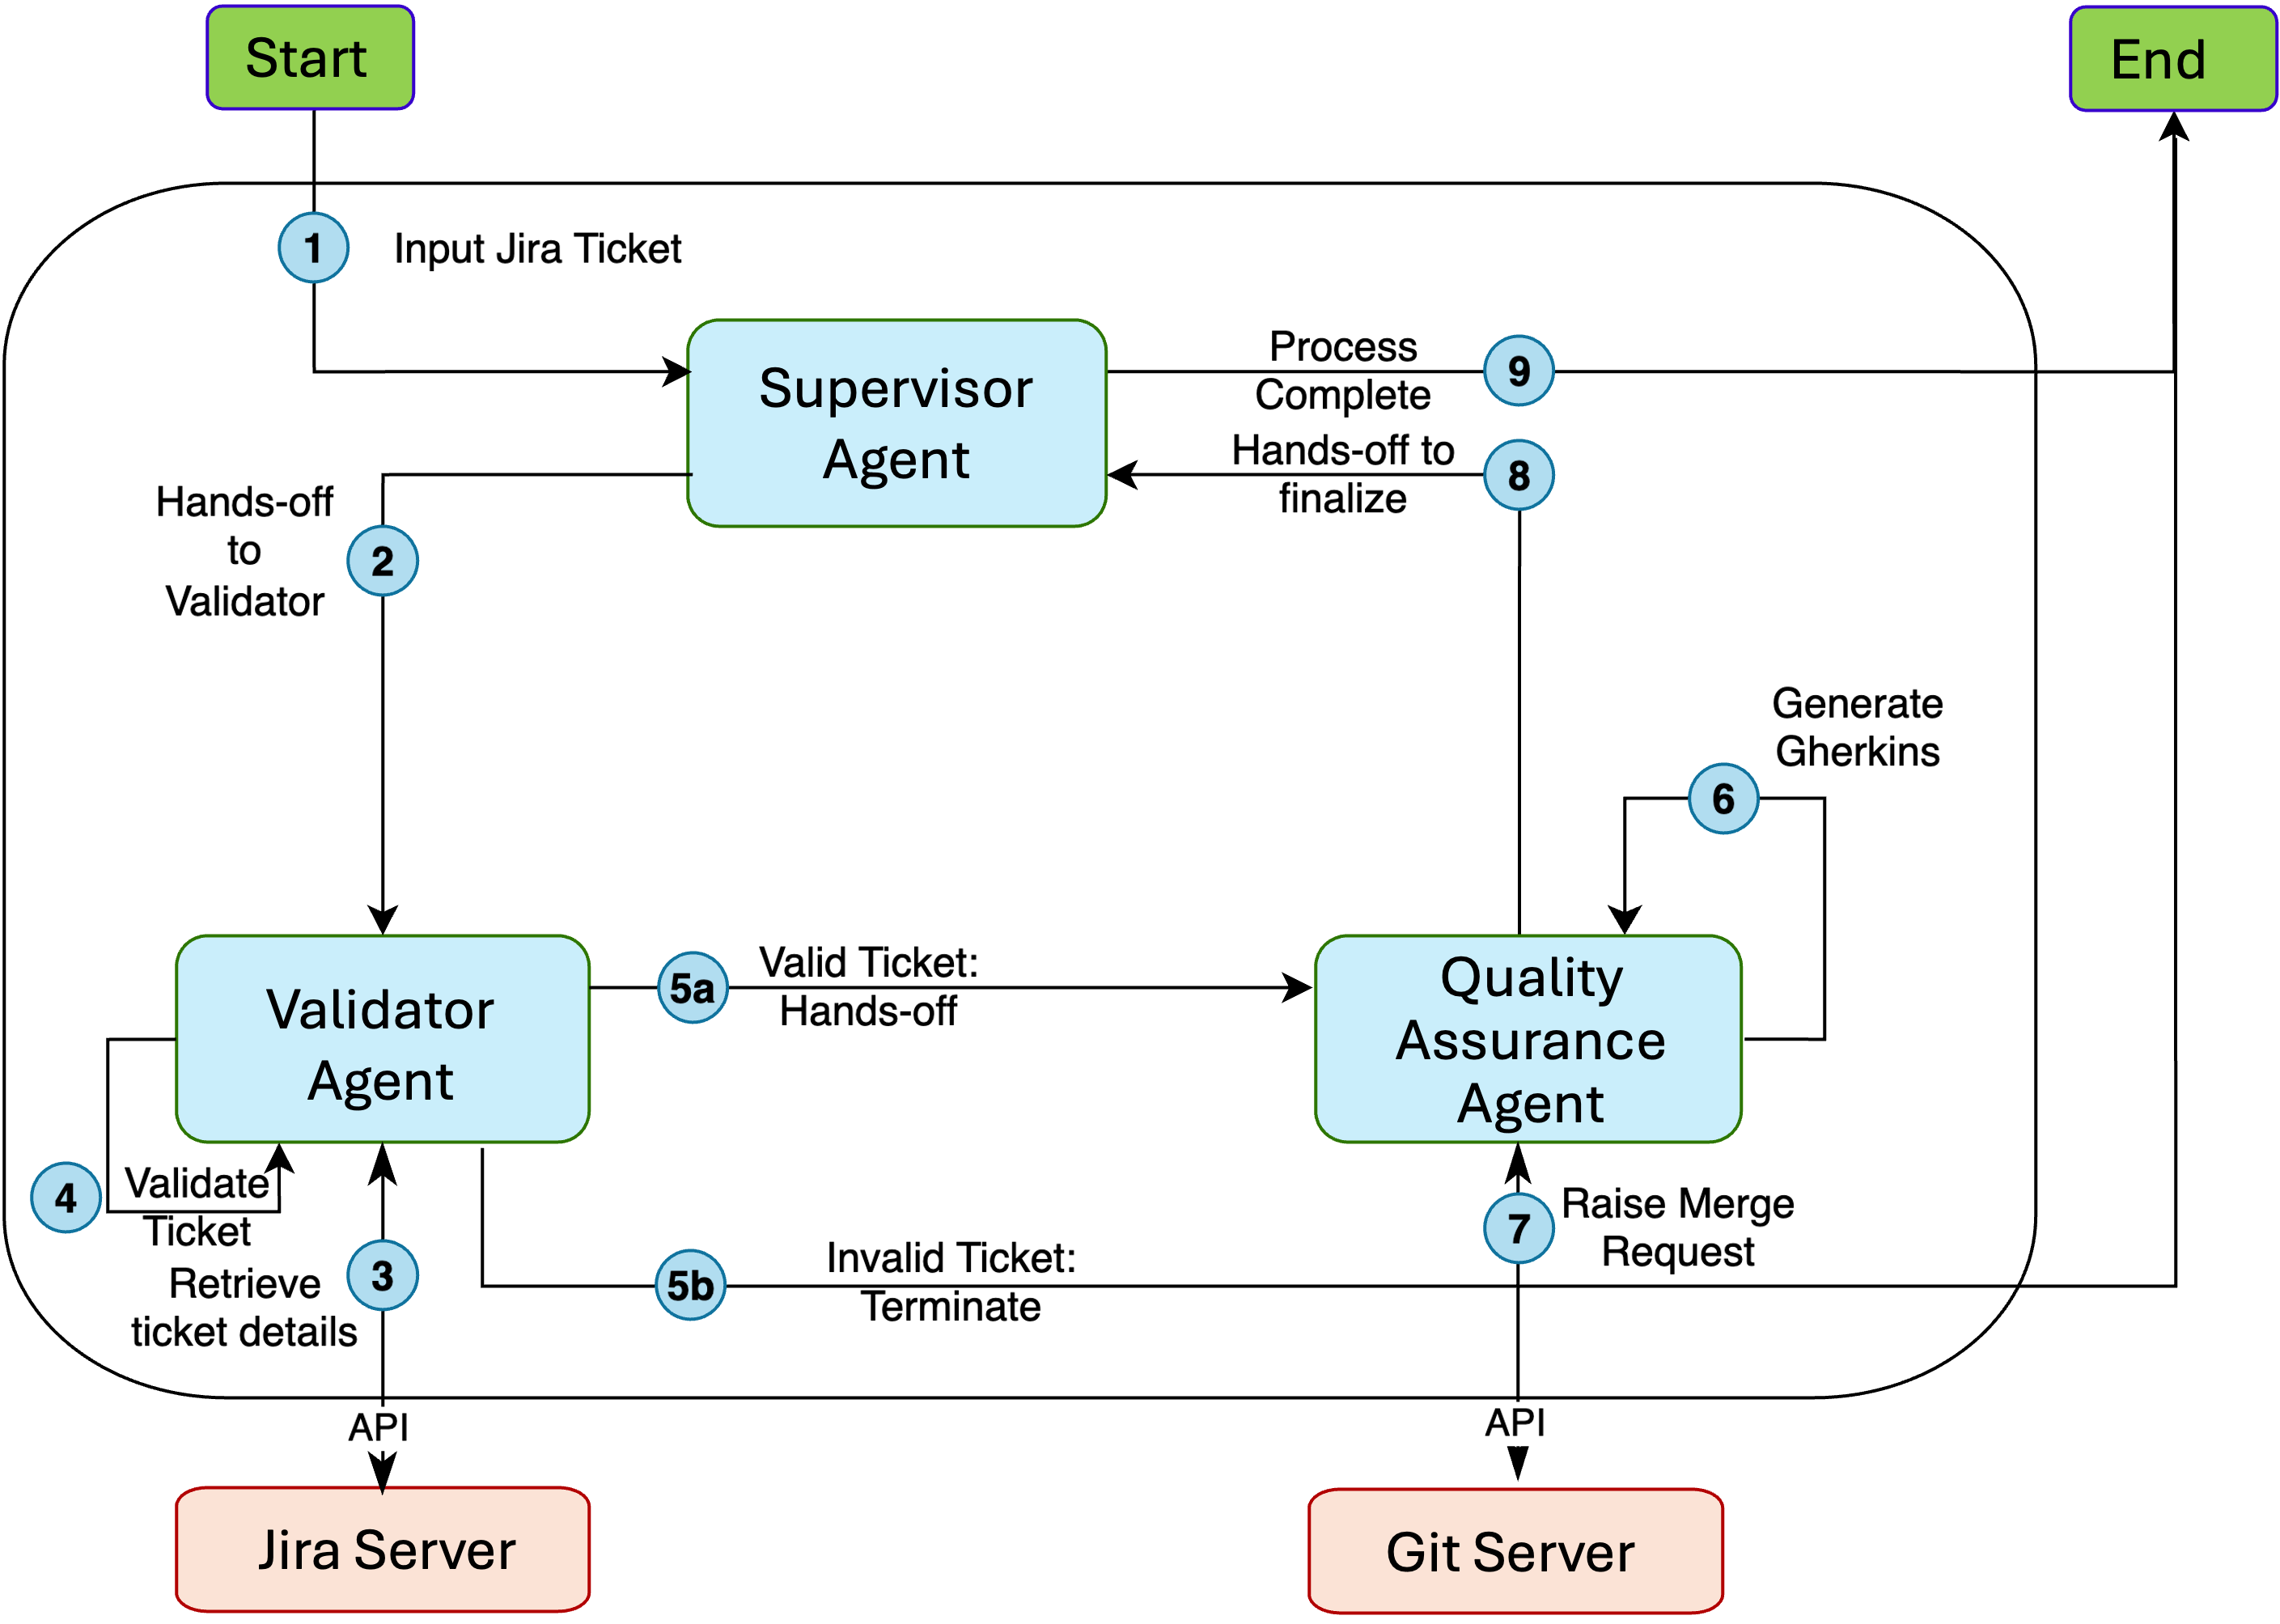
\includegraphics[width=\linewidth]{figures/architecture-v5.png}
\caption{Architecture and operational workflow of CMAS4G2. The diagram illustrates the nine-step process involving the Supervisor, Validator, and Quality Assurance agents.}
\label{fig:MAS-design}
\end{figure}

CMAS4G2 leverages Microsoft's AutoGen Swarm framework to orchestrate interactions among three specialized agents:

\begin{itemize}[leftmargin=*]
    \item \textbf{Supervisor Agent:} Acts as the central orchestration component, managing workflow execution and ensuring correct handoffs between specialized agents.
    \item \textbf{Validator Agent:} Focuses on Jira ticket analysis and content validation. This agent establishes direct API connectivity with Jira to retrieve ticket data and perform systematic validation checks.
    \item \textbf{Quality Assurance Agent:} Transforms validated requirements into executable Gherkin acceptance tests, combining domain knowledge in test design patterns with automated code generation capabilities.
\end{itemize}

The end-to-end workflow proceeds through the following phases:

\begin{enumerate}[leftmargin=*]
    \item \textbf{Initialization Phase:} The Supervisor Agent receives the input Jira ticket and orchestrates its handoff to the Validator Agent.
    \item \textbf{Validation Phase:} The Validator Agent retrieves ticket details via the Jira API and performs content validation. Tickets that fail validation are rejected with documented deficiencies.
    \item \textbf{Generation Phase:} Upon successful validation, the Quality Assurance Agent generates Gherkin test scripts and creates automated merge requests in Git.
    \item \textbf{Completion Phase:} The Supervisor Agent manages the final coordination steps and concludes the workflow.
\end{enumerate}

\subsection{Evaluation Framework}

We employ the LLM-as-a-Judge (LAJ) framework from Section~\ref{sec:llm_judge} for evaluating generated Gherkin scripts, using GPT-4o Mini as the judge model following calibration against expert human annotations. This integration demonstrates the practical utility of the LAJ framework for downstream agentic applications.

\subsubsection{Dataset}

The benchmark comprises 200 synthetic Jira tickets based on the open-source Kill Bill subscription billing platform:
\begin{itemize}[leftmargin=*]
    \item \textbf{Valid Tickets (IDs 1--100):} Complete tickets for successful Gherkin generation
    \item \textbf{Invalid Tickets (IDs 101--200):} Deliberately incomplete tickets to test rejection logic
\end{itemize}

\subsubsection{Performance Metrics}

\begin{itemize}[leftmargin=*]
    \item \textbf{Valid Ticket Success Rate:} Percentage of well-formed tickets for which the system successfully generates Gherkin scripts
    \item \textbf{Invalid Ticket Success Rate:} Percentage of incomplete tickets correctly rejected before test generation
    \item \textbf{Overall Success Rate:} Combined success: (Valid SR + Invalid SR)/2
    \item \textbf{Average Test Coverage:} Mean coverage score assigned by the LAJ framework
\end{itemize}

\subsection{Results}

Table~\ref{tab:cmas4g2_results} presents performance across model configurations.

\begin{table}[htbp]
\centering
\caption{CMAS4G2 Performance on 200-Ticket Kill Bill Benchmark. Values are mean$\pm$std across 5 runs.}
\label{tab:cmas4g2_results}
\resizebox{\textwidth}{!}{%
\begin{tabular}{@{}llcccc@{}}
\toprule
\textbf{Model} & \textbf{Config} & \textbf{Valid (\%)} & \textbf{Invalid (\%)} & \textbf{Overall (\%)} & \textbf{Coverage (\%)} \\
\midrule
Claude Sonnet 4 & -- & \textbf{100.0$\pm$0} & \textbf{80.8$\pm$0} & \textbf{90.4$\pm$0} & \textbf{91.6$\pm$0} \\
\midrule
\multirow{2}{*}{GPT-OSS 20B} & medium & 99.2$\pm$2 & 76.0$\pm$0 & 87.6$\pm$1 & 85.4$\pm$0 \\
 & high & 1.6$\pm$3 & 73.0$\pm$0 & 37.3$\pm$2 & 16.8$\pm$34 \\
\midrule
\multirow{2}{*}{Qwen3-32B} & no think & 99.2$\pm$1 & 35.2$\pm$0 & 67.2$\pm$1 & 86.9$\pm$0 \\
 & think & 87.2$\pm$5 & 69.0$\pm$0 & 78.1$\pm$2 & 83.7$\pm$0 \\
\midrule
\multirow{2}{*}{Qwen3-8B} & no think & 58.8$\pm$24 & 41.0$\pm$0 & 49.9$\pm$12 & 79.5$\pm$3 \\
 & think & 98.0$\pm$2 & 57.0$\pm$0 & 77.5$\pm$1 & 79.2$\pm$0 \\
\bottomrule
\end{tabular}
}
\end{table}

\subsubsection{Key Findings}

\textbf{Open-Weight Models Approach Proprietary Performance.} GPT-OSS 20B (medium) achieves 87.6\% overall success and 85.4\% coverage, approaching within 2.8 percentage points of Claude Sonnet 4's 90.4\% and 91.6\% while enabling fully local deployment.

\textbf{Reasoning Configuration Critically Affects Quality.} The impact of reasoning mode varies dramatically by model size:
\begin{itemize}[leftmargin=*]
    \item \textbf{Small models benefit dramatically:} Qwen3-8B improves from 49.9\% to 77.5\% overall success with thinking mode---a 27.6 percentage point gain
    \item \textbf{Large models show mixed effects:} Qwen3-32B degrades from 99.2\% to 87.2\% valid ticket success with thinking mode, while improving invalid ticket rejection from 35.2\% to 69.0\%
    \item \textbf{Excessive reasoning causes catastrophic failure:} GPT-OSS 20B (high) collapses to 1.6\% valid success due to context exhaustion before completing Gherkin generation
\end{itemize}

These reasoning configuration findings directly inform Chapter~\ref{ch:strategies}, where we systematically characterize the relationship between reasoning intensity and task complexity across sentiment analysis tasks.

\textbf{Invalid Ticket Rejection Remains Challenging.} All models struggle with invalid ticket rejection compared to valid ticket processing. Claude Sonnet 4 achieves only 80.8\% rejection rate, with open-weight models ranging from 35.2\% to 76.0\%. This asymmetry suggests that correctly identifying \textit{missing} information is harder than processing \textit{present} information.

\subsection{Integration Summary}

The successful integration of CMAS4G2 with the LAJ framework demonstrates the practical value of our multi-dimensional evaluation approach. By establishing ECR@1 and adjusted cost metrics in Section~\ref{sec:llm_judge}, we enabled reliable, cost-effective evaluation of generated tests at scale---a critical capability for operationalizing automated test generation in enterprise CI/CD pipelines.

%% =============================================================================
%% PART 3: Standalone Systems (Papers 5-6)
%% =============================================================================

\section{Hierarchical Multi-Agent System for Payments}
\label{sec:hmasp}

While the preceding sections focus on back-office automation and software quality assurance, payment processing presents distinct challenges: traditional payment infrastructure employs anti-bot mechanisms, multi-factor authentication, and fraud detection systems that constrain agentic technology adoption. This section presents HMASP (Hierarchical Multi-Agent System for Payments)~\cite{huang2026hmasp}, the first LLM-based multi-agent system to implement end-to-end agentic payment workflows.

\subsection{Architecture Overview}

HMASP addresses end-to-end agentic payment processing through a modular, four-level hierarchical design implemented using LangGraph~\cite{langchain2024langgraph}. Figure~\ref{fig:MAS-design} illustrates the architecture.

\begin{figure}[!h]
    \centering
    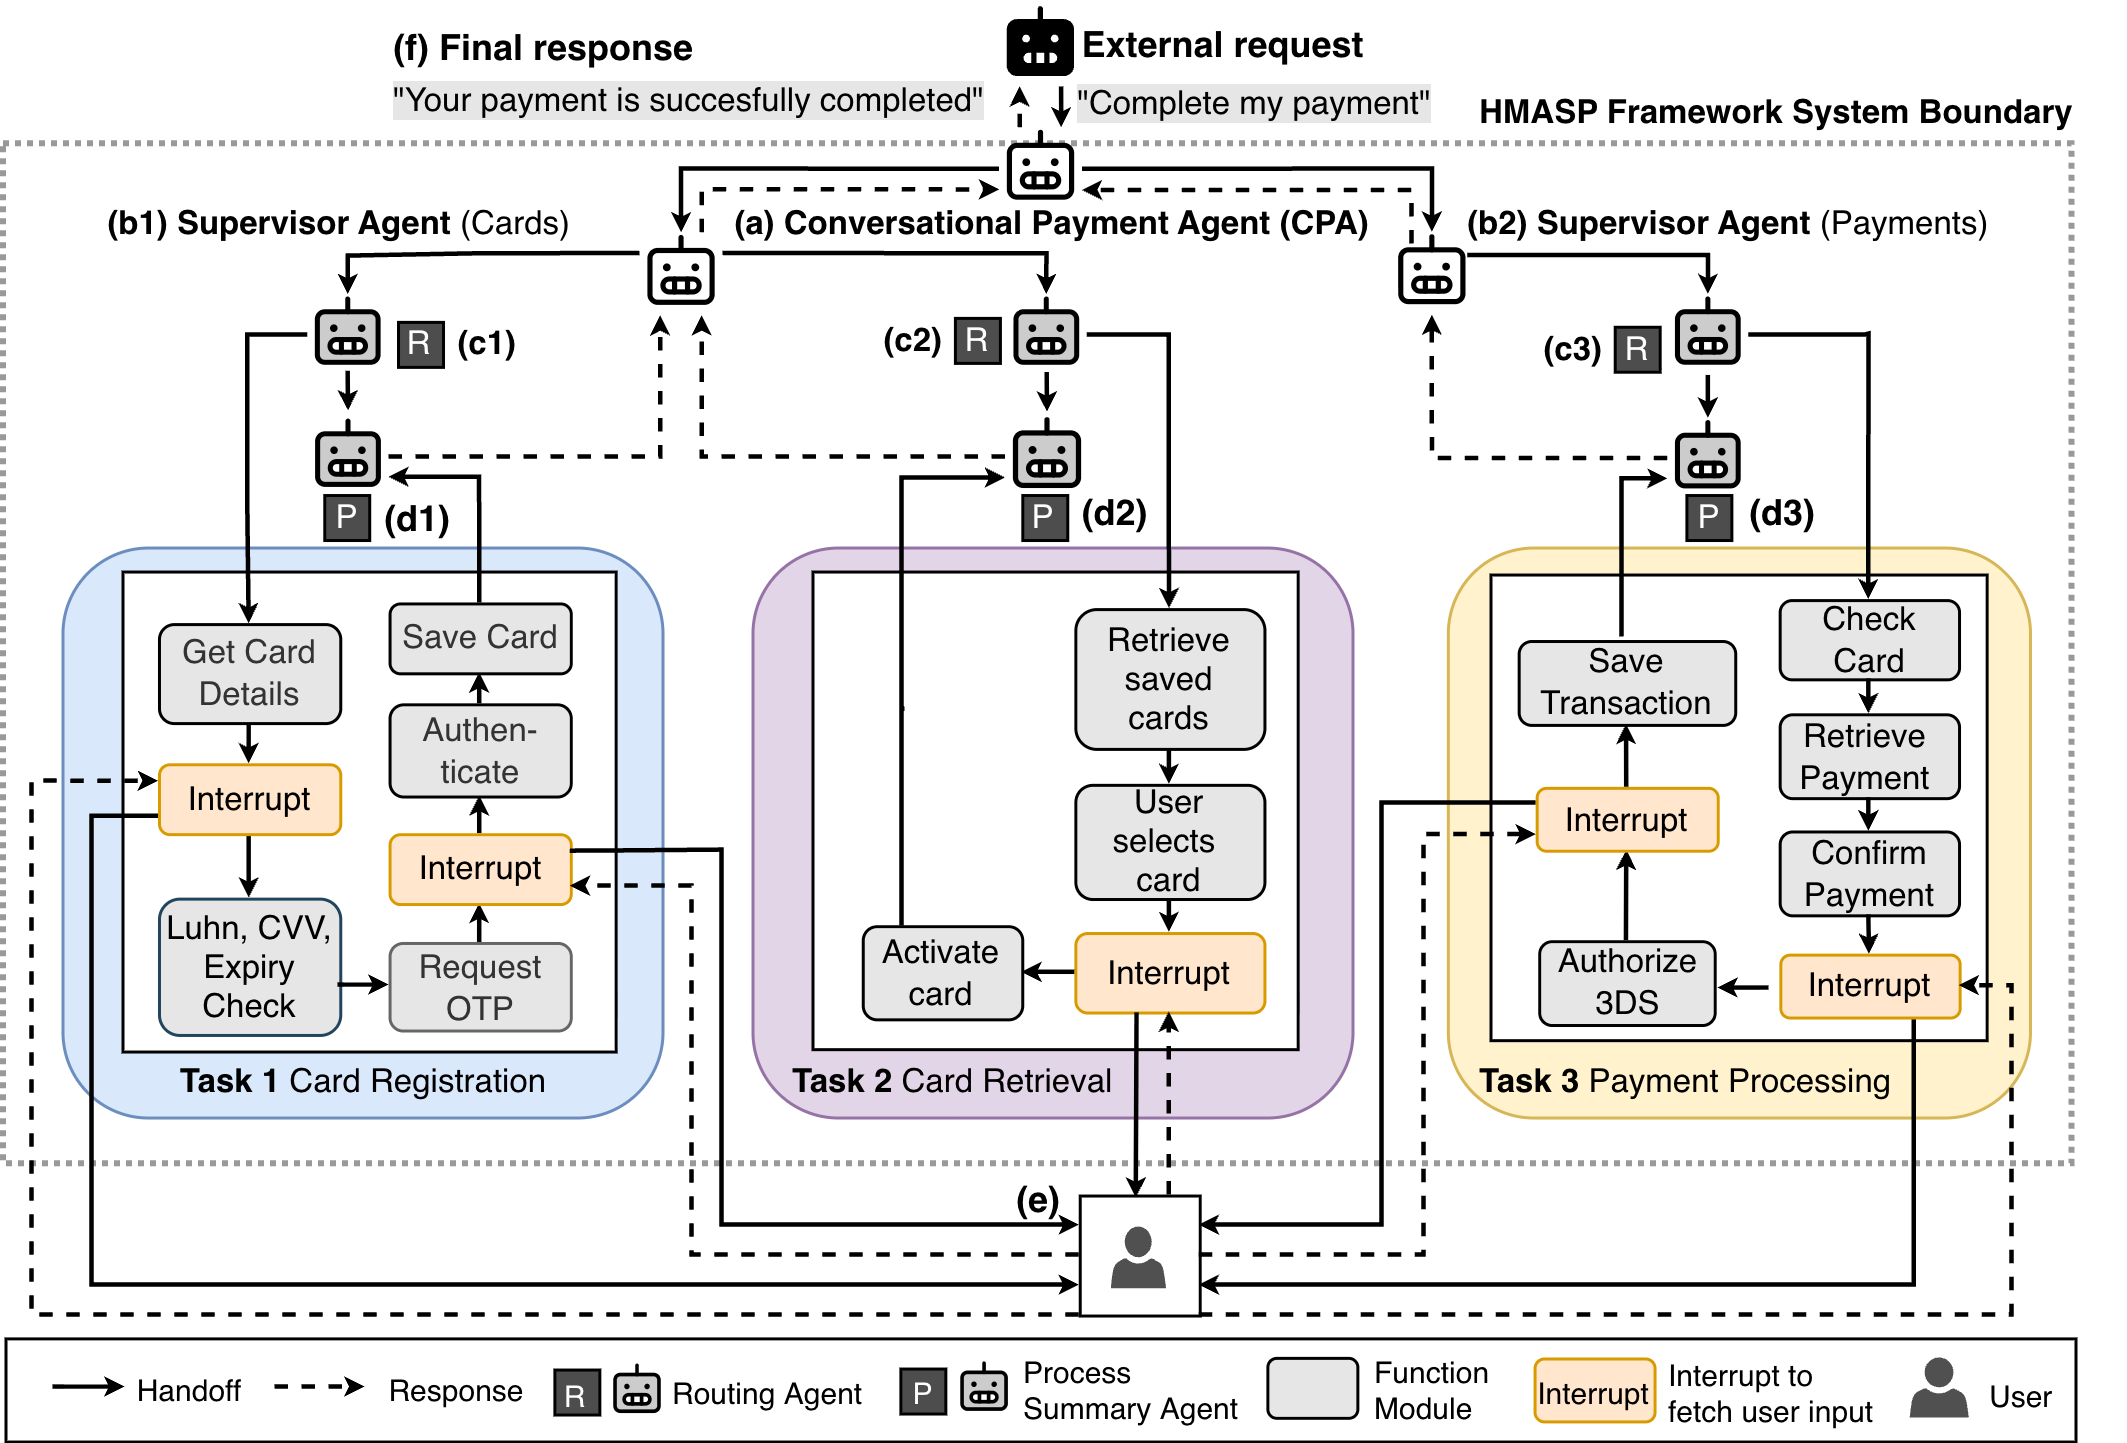
\includegraphics[width=\textwidth]{figures/ConvPayAgent6.png}
    \caption{Overview of the proposed HMASP. An external request (e.g., ``Complete my payment'') is sent to the Conversational Payment Agent (CPA - first agent level);
    (a) The CPA processes the request and delegates it to one of the two Supervisors (b1, b2 - second agent level) for further handling;
    (b) The selected Supervisor routes the request to a suitable Routing agent (c1, c2, or c3 - third agent level);
    (c) Routing agents initiate the corresponding task-specific workflow (Task 1, Task 2, Task 3);
    Upon initiation, a series of task-relevant function modules are triggered to complete the request;
    (d) Upon task completion, the Process summary agent (d1, d2, d3 - fourth agent level) compiles the outcome and generates a response. This summary response is propagated upward the system hierarchy through Supervisor agents and CPA;
    (e) When user input is required to complete the task, an interrupt mechanism is triggered to obtain the necessary input before execution resumes;
    (f) Finally, the CPA responds to the request (e.g., ``Your payment has been successfully completed'').
    }
    \label{fig:MAS-design}
\end{figure}

\subsubsection{Agent Hierarchy}

The hierarchy comprises four distinct agent levels:

\begin{enumerate}[leftmargin=*]
    \item \textbf{Conversational Payment Agent (CPA):} Primary orchestrator receiving external requests. The CPA handles all incoming requests and coordinates task delegation to supervisors. It can also reject irrelevant requests.
    
    \item \textbf{Supervisor Agents:} Decision-makers that delegate requests based on context and workload to appropriate sub-workflows. Each supervisor is responsible for reporting outcomes back to the CPA.
    
    \item \textbf{Routing Agents:} Identify and initiate task-specific workflows. They serve as the final decision layer on whether to trigger payment-related function modules or reject irrelevant requests.
    
    \item \textbf{Process Summary Agents:} Interact with underlying systems to execute operations and generate structured responses on workflow outcomes.
\end{enumerate}

\subsubsection{Architectural Patterns}

HMASP incorporates several architectural patterns ensuring reliable payment processing:

\textbf{Shared State Variables:} Graph States consist of user-defined variables that persist throughout MAS runtime. Agents can only access their assigned states, preventing unauthorized read/write across state variables.

\textbf{Information Determinism:} Critical payment information is stored in state variables rather than generated by LLMs. This decouples payment-related processing from generative processes---payment amounts, card numbers, and transaction IDs are retrieved from state variables, never hallucinated.

\textbf{Structured Handoffs:} Agents use LangGraph's handoff mechanism to seamlessly pass processes to one another, enabling coordination where requests flow from CPA through the hierarchy.

\textbf{Interrupt Mechanism:} When user input is required during execution (e.g., OTP verification, card selection), an interrupt mechanism pauses the workflow to collect necessary input before proceeding.

\subsection{Evaluation}

We constructed a dataset of 1,000 payment-related inputs across four task categories: Card Registration (250), Card Retrieval (250), Payment Checkout (250), and Irrelevant Inputs (250).

\subsection{Results}

Table~\ref{tab:hmasp_results} presents task success rates across models.

\begin{table}[htbp]
\centering
\caption{HMASP Task Success Rates (\%) Across Models}
\label{tab:hmasp_results}
\begin{tabular}{@{}lcccc@{}}
\toprule
\textbf{Model} & \textbf{Task 1} & \textbf{Task 2} & \textbf{Task 3} & \textbf{Task 4} \\
\midrule
GPT-4.1 (Baseline) & \textbf{99.6} & \textbf{99.6} & \textbf{99.6} & \textbf{100.0} \\
Qwen2.5:32b & 97.2 & 98.4 & 98.8 & 100.0 \\
Qwen2.5:14b & 94.0 & 95.2 & 98.8 & 100.0 \\
Qwen3:32b & 99.6 & 35.2 & 39.6 & 100.0 \\
Mistral-small3.2:24b & 94.8 & 94.0 & 82.8 & 100.0 \\
Llama3.1:70b & 87.2 & 88.4 & 47.2 & 33.2 \\
Llama3.1:8b & 38.0 & 38.4 & 39.2 & 3.6 \\
\bottomrule
\end{tabular}
\end{table}

\subsubsection{Key Findings}

\textbf{Open-Source Viability:} Qwen2.5:32b achieves an average 97.0\% task success rate across payment-relevant tasks (Tasks 1--3), demonstrating viability for end-to-end agentic payments with open-weight models.

\textbf{Inconsistent Performance Across Tasks:} Some models show inconsistent behavior---Qwen3:32b achieves 99.6\% on Task 1 but only 35.2\% and 39.6\% on Tasks 2 and 3, indicating that strong performance on one task does not guarantee reliability across the workflow.

\textbf{Irrelevant Input Handling:} Most models correctly reject irrelevant inputs (Task 4), with Qwen2.5 variants achieving 100\%. However, Llama3.1 models showed weakness, with Llama3.1:8b achieving only 3.6\%.

\subsection{Novelty and Contributions}

To our knowledge, HMASP is the first LLM-based multi-agent system supporting fully end-to-end agentic payment workflows. Table~\ref{tab:comparative-study-table} provides comparative analysis with existing approaches.

\begin{table}[!h]
  \centering
  \begin{threeparttable}
  \begin{tabular}{
      p{0.18\linewidth}%
      >{\centering\arraybackslash}p{0.10\linewidth}%
      >{\centering\arraybackslash}p{0.12\linewidth}%
      >{\centering\arraybackslash}p{0.12\linewidth}%
      >{\centering\arraybackslash}p{0.15\linewidth}%
      >{\centering\arraybackslash}p{0.12\linewidth}
    }
    \toprule
    \textbf{Method} & \textbf{Open-Weight LLM} & \textbf{Full Payment Processing} & \textbf{TR Success Rate (\%)} & \textbf{TR Precision-Recall (\%)} & \textbf{TR F1-Score (\%)} \\
    \midrule
    LLMPA~\cite{guan2024llmprocessautomation} & Yes & No\tnote{1} & 76.5 & -- & -- \\
    Method 1~\cite{dahiphale2024llmscampayments} & No & No & 93.3 & 85.7--30.2 & 44.77 \\
    Method 2~\cite{qu-etal-2025-llm-fraud} & Yes & No & -- & N/A\tnote{2}--73.7 & -- \\
    \midrule
    \textbf{HMASP (Ours)} & \textbf{Yes} & \textbf{Yes} & \textbf{97.7} & \textbf{99.4--98.8} & \textbf{99.2} \\
    \bottomrule
  \end{tabular}
  \begin{tablenotes}
    \small
    \item[1] Processing stops at network boundary; defaults to in-app checkout.
    \item[2] Not reported.
  \end{tablenotes}
  \caption{A comparative overview of existing autonomous agents in payment-relevant processes with their Task-Relevant (TR) metrics. For HMASP, averages from the best-performing open-weight LLM (Qwen2.5:32b) were reported.}
  \label{tab:comparative-study-table}
  \end{threeparttable}
\end{table}

%% =============================================================================
%% Section: EdgeAgent - Semi-Automatic Annotation Pipeline
%% =============================================================================

\section{EdgeAgent and Agentic Success Rate: Semi-Automatic Annotation with Reliability Metrics}
\label{sec:edgeagent}

This section presents EdgeAgent~\cite{huang2026edgeagent}---a semi-automatic data labeling pipeline that orchestrates tool-using LLMs on edge devices for specialized domain annotation. A central contribution is the \textbf{Agentic Success Rate (ASR)} metric, which provides fine-grained evaluation of tool-calling precision throughout multi-step workflows, complementing the 12-category error taxonomy introduced in Section~\ref{sec:diagnostic_framework}. Using maritime risk assessment as a case study, we evaluate 14 open-source Qwen models (0.5B--72B) against GPT-4.1 variants across three hardware platforms, demonstrating that open-source models can achieve production-quality annotation while preserving privacy.

\subsection{Motivation}

Data labeling and annotation constitute critical bottlenecks in machine learning pipelines, particularly for specialized domains requiring expert knowledge~\cite{huang2024automating}. Maritime risk assessment exemplifies these challenges: incidents span diverse categories (weather events, accidents, cyber attacks, administrative issues), require domain expertise to classify correctly, and emerge continuously from news sources worldwide. Traditional manual annotation approaches are labor-intensive, expensive, and struggle to scale with the volume and velocity of incoming data.

Privacy concerns may prohibit sending sensitive data to cloud APIs, latency requirements demand local processing, and resource constraints on edge devices limit model selection. Furthermore, annotation pipelines require more than classification---they need tool integration for data retrieval, content extraction, multi-step reasoning, and database operations.

\subsection{Semi-Automatic Labeling Pipeline Architecture}

The EdgeAgent pipeline implements an interactive workflow where researchers submit URLs of news articles and receive automated annotations through LLM-orchestrated tool calls. Figure~\ref{fig:edgeagent_architecture} illustrates the architecture.

\begin{figure}[htbp]
    \centering
    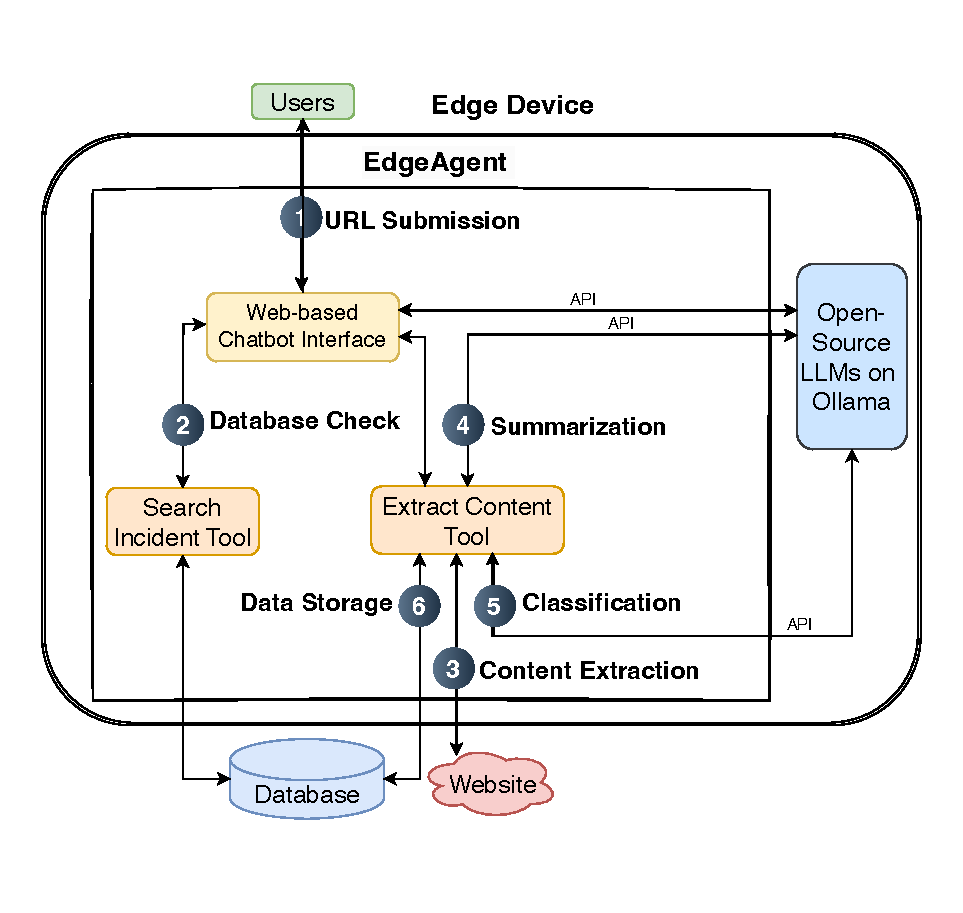
\includegraphics[width=\textwidth]{images/Edge_AI_Agents_v5.drawio.pdf}
    \caption{EdgeAgent Architecture: Semi-Automatic Data Labeling Pipeline. The system orchestrates LLM-powered agents for (1) URL submission, (2) database checking, (3) content extraction, (4) summarization, (5) classification, and (6) data storage. Open-source LLMs run locally on edge devices, enabling privacy-preserving annotation without cloud dependency.}
    \label{fig:edgeagent_architecture}
\end{figure}

The semi-automatic workflow consists of six key steps:

\begin{enumerate}[leftmargin=*]
    \item \textbf{URL Submission:} Researchers submit URLs through a web-based interface, initiating the annotation process.
    \item \textbf{Database Check:} EdgeAgent queries the database to avoid duplicate labeling, retrieving existing annotations if available.
    \item \textbf{Content Extraction:} An integrated tool extracts textual content from submitted URLs, handling diverse web formats.
    \item \textbf{Summarization:} Selected LLMs generate concise summaries emphasizing incident details, location, and consequences.
    \item \textbf{Classification:} LLMs classify summarized content into predefined risk categories using few-shot prompting.
    \item \textbf{Data Storage and Retrieval:} Annotated data is stored in a structured database, enabling interactive queries and visualization.
\end{enumerate}

Beyond automated annotation, EdgeAgent's agentic architecture enables researchers to interactively query the accumulated database using natural language and manually update labels when automated classifications require refinement.

\subsection{Agentic Success Rate: Evaluating Annotation Pipeline Reliability}

In automated labeling systems, LLMs must correctly orchestrate multiple tools across workflow steps. Traditional binary metrics (task success/failure) can mask partial failures where some annotation steps succeed while others fail. To address this limitation, we introduce the \textbf{Agentic Success Rate (ASR)}---a fine-grained metric quantifying tool-calling precision throughout multi-step workflows.

\subsubsection{Metric Definition}

We formalize ASR by decomposing agentic workflows into atomic evaluation steps. For a pipeline with $n$ evaluable steps, let $S_i \in \{0, 1\}$ indicate successful completion of step $i$. The Overall Agentic Score (OAS) aggregates these indicators:

\begin{equation}
\text{OAS} = \sum_{i=1}^{n} w_i \cdot S_i
\end{equation}

where $w_i$ represents developer-defined weights (default: 1). The Agentic Success Rate normalizes this score:

\begin{equation}
\text{ASR} = \frac{\text{OAS}}{\sum_{i=1}^{n} w_i}
\end{equation}

An ASR of 1.00 (100\%) indicates flawless pipeline execution; lower scores pinpoint specific failure modes. For example, a model correctly invoking both tools but mishandling URL transmission at step $S_5$ yields OAS=4, ASR=0.57---revealing partial success that binary metrics would score as complete failure.

\subsubsection{Generality of the Framework}

Although demonstrated with maritime annotation, ASR applies to arbitrary agentic architectures. In general, agent execution forms a directed acyclic graph (DAG) where internal nodes represent reasoning states and leaf nodes are tool calls. During execution, the LLM traverses a path through this DAG, with each edge terminating in one or more tool invocations.

Because dispatch logic is developer-controlled, every call and sub-step can be logged, time-stamped, and scored at arbitrary granularity. The framework is computed by:
\begin{enumerate}[leftmargin=*]
    \item Enumerating evaluable sub-steps along the observed traversal
    \item Assigning developer-defined weights and error categories
    \item Normalizing by the path's maximum attainable score
\end{enumerate}

This design enables consistent evaluation across chains, trees, or complex DAGs while preserving step-level diagnostics comparable across diverse architectures and domains.

\subsubsection{Application to EdgeAgent}

The EdgeAgent pipeline employs two tools: \texttt{search\_incident} (database lookup) and \texttt{extract\_content} (web scraping). We decompose each labeling task into seven atomic steps ($S_i$, where $i = 1, 2, \ldots, 7$):

\begin{itemize}[leftmargin=*]
    \item[$S_1$] Invocation of \texttt{search\_incident}
    \item[$S_2$] Transmission of the URL parameter to \texttt{search\_incident}
    \item[$S_3$] Execution of the database query
    \item[$S_4$] Invocation of \texttt{extract\_content}
    \item[$S_5$] Transmission of the URL parameter to \texttt{extract\_content}
    \item[$S_6$] Completion of summarization
    \item[$S_7$] Completion of classification (label generation)
\end{itemize}

The stepwise breakdown provides actionable insights for improving labeling pipelines. Tool invocation failures ($S_1$, $S_4$) indicate prompt engineering issues or insufficient model capacity for structured workflows. Parameter transmission errors ($S_2$, $S_5$) reveal hallucination problems where models generate invalid tool arguments. Processing failures ($S_6$, $S_7$) suggest downstream component issues or data quality problems. This granularity guides targeted improvements, distinguishing orchestration failures (fixable through better prompting) from fundamental model limitations (requiring larger models).

\subsection{Experimental Setup}

\paragraph{Model Integration.} We evaluate OpenAI models (GPT-4.1-nano, GPT-4.1-mini, GPT-4.1) and open-source models (Qwen 2.5: 0.5B--72B, Qwen 3: 0.6B--32B). Qwen3 models support dual-mode reasoning: thinking mode enables complex multi-step reasoning, while non-thinking mode provides rapid responses.

\paragraph{Dataset.} We collected 2,232 maritime news articles, curating 1,003 articles for evaluation after filtering. Ground truth labels were obtained with GPT-4o and refined through human review.

\paragraph{Hardware Configurations.} Testing across three platforms: NVIDIA H100 (enterprise), NVIDIA RTX 4090 (consumer GPU), and Apple M3 Max (portable edge device).

\subsection{Results}

Table~\ref{tab:edgeagent_results_full} presents comprehensive evaluation results.

\begin{table}[htbp]
\centering
\caption{EdgeAgent Model Performance for Semi-Automatic Data Labeling. For Qwen3 models, (T) denotes thinking mode and (N) denotes standard mode. All Qwen results obtained on H100 platform.}
\label{tab:edgeagent_results_full}
\begin{tabular}{@{}lcccc@{}}
\toprule
\textbf{Model} & \textbf{ASR (\%)} & \textbf{TSR (\%)} & \textbf{F1 (\%)} & \textbf{MRT (s)} \\
\midrule
\multicolumn{5}{l}{\textit{Qwen Models (Selected)}} \\
qwen2.5:7b & 74.48 & 60.32 & 81.88 & 12.8 \\
qwen2.5:14b & 76.88 & 75.57 & 83.38 & 15.3 \\
qwen2.5:32b & 93.36 & 93.32 & 82.45 & 15.1 \\
qwen2.5:72b & 94.99 & 93.12 & \textbf{86.19} & 38.7 \\
qwen3:32b (T) & \textbf{98.21} & \textbf{97.21} & 82.98 & 36.0 \\
qwen3:32b (N) & 84.29 & 74.88 & 83.17 & 28.9 \\
\midrule
\multicolumn{5}{l}{\textit{OpenAI Models}} \\
GPT-4.1-nano & 98.08 & 99.40 & 65.55 & \textbf{7.3} \\
GPT-4.1-mini & 99.49 & 99.60 & \textbf{86.17} & 13.4 \\
GPT-4.1 & \textbf{99.91} & \textbf{100.00} & 83.61 & 14.1 \\
\bottomrule
\end{tabular}
\end{table}

\subsubsection{Key Findings}

\textbf{Open-Source Models Match Proprietary Quality.} qwen3:32b (T) achieves 98.21\% ASR, 97.21\% TSR, and 82.98\% F1---performance nearly matching GPT-4.1. This demonstrates that local, privacy-preserving annotation pipelines can deliver quality comparable to cloud-based proprietary alternatives.

\textbf{Model Size Determines Annotation Reliability.} Smaller models ($<$4B) exhibit significant disparities between task completion and proper workflow execution. For example, qwen3:0.6b achieves 84.35\% TSR but only 0.10\% ASR, indicating it bypasses required database lookup steps rather than following proper annotation protocols.

\textbf{Thinking Mode Enhances Multi-Step Annotation.} qwen3:32b (T) achieves 98.21\% ASR compared to 84.29\% in non-thinking mode---a 14-point difference demonstrating the value of extended reasoning for complex workflows. This finding connects directly to the reasoning configuration analysis in Chapter~\ref{ch:strategies}, where we characterize the Reasoning Intensity (RI) metric and its relationship to task complexity.

\textbf{Annotation Quality is Hardware-Independent.} All platforms exhibit consistent ASR and TSR patterns across models. Model selection governs annotation quality, while hardware determines throughput. qwen2.5:32b completes tasks in 15s on H100, compared to 169s on RTX 4090 and 296s on M3 Max---representing 11.3$\times$ and 19.7$\times$ speedups respectively.

\subsection{Diagnostic Value and Cross-Domain Applicability}

The ASR metric and its application to EdgeAgent validate the cross-domain applicability of fine-grained reliability evaluation. The same diagnostic principles apply across domains:

\begin{itemize}[leftmargin=*]
    \item Tool-calling errors dominate failures for smaller models
    \item Processing quality remains consistent once workflows are properly initiated
    \item The three-tier deployment guidance (${<}$4B unsuitable, 7B--14B transitional, ${\geq}$32B production-ready) generalizes across applications
\end{itemize}

Combined with the 12-category error taxonomy from Section~\ref{sec:diagnostic_framework}, ASR provides comprehensive diagnostics for multi-agent LLM systems---enabling practitioners to systematically diagnose failure modes and guide targeted improvements.

%% =============================================================================
%% Practical Guidelines and Summary
%% =============================================================================

\section{Practical Deployment Guidelines}
\label{sec:agentic_guidelines}

Based on our research across six systems, we provide consolidated guidelines for enterprise agentic AI deployment:

\subsection{Architecture Design}

\begin{enumerate}[leftmargin=*]
    \item \textbf{Modular agent specialization:} Design agents with clearly defined, focused responsibilities
    \item \textbf{Hierarchical coordination:} Employ multi-level hierarchies for complex workflows, enabling modular task execution
    \item \textbf{Information determinism:} Store critical information in state variables, not LLM outputs, preventing hallucination of sensitive data
    \item \textbf{Structured handoffs:} Implement clear protocols for inter-agent communication
    \item \textbf{Human oversight:} Incorporate validation checkpoints for high-impact decisions
\end{enumerate}

\subsection{Model Selection}

\begin{enumerate}[leftmargin=*]
    \item \textbf{Large models ($\geq$32B):} Provide production-ready reliability (ASR $>$93\%) for autonomous workflows
    \item \textbf{Mid-tier models (7B--14B):} Suitable for interactive workflows with human review, balancing accuracy and latency
    \item \textbf{Small models ($<$4B):} Unsuitable for multi-step agentic pipelines despite acceptable performance on isolated tasks
    \item \textbf{Consider edge deployment:} Reduces latency, improves privacy, and eliminates API costs---qwen2.5:32b matches proprietary performance while enabling local deployment
\end{enumerate}

\subsection{Reliability Engineering}

\begin{enumerate}[leftmargin=*]
    \item \textbf{Measure ECR@1:} Always capture first-attempt success rates alongside accuracy
    \item \textbf{Implement retry logic:} Budget 5--15\% overhead for reliability failures
    \item \textbf{Monitor operational metrics:} Track ECR@1, latency, and cost in production
    \item \textbf{Use adjusted cost metrics:} Account for retry overhead in total cost of ownership
\end{enumerate}

\subsection{Evaluation Strategy}

\begin{enumerate}[leftmargin=*]
    \item \textbf{Use fine-grained metrics:} Adopt ASR or similar stepwise metrics to diagnose failure modes beyond binary success/failure
    \item \textbf{Distinguish orchestration from processing:} Tool-calling failures require different interventions than classification errors
    \item \textbf{Hardware-aware benchmarking:} Test on target deployment hardware to establish realistic performance expectations
    \item \textbf{Multi-dimensional evaluation:} Assess accuracy, reliability, and cost together for production readiness
\end{enumerate}

\section{Summary}
\label{sec:agentic_summary}

This chapter demonstrated the viability and effectiveness of agentic AI for automating complex enterprise workflows, addressing the second research question (RQ2) on designing and evaluating multi-agent LLM systems for reliable, scalable enterprise automation. Key contributions include:

\begin{enumerate}[leftmargin=*]
    \item \textbf{Multi-agent invoice reconciliation (Section~\ref{sec:invoice_reconciliation}):} Validated architecture achieving 99.9\% success rate with edge-deployed open-source models, demonstrating that qwen2.5:32b outperforms proprietary alternatives while consuming only 523J per task on consumer hardware
    
    \item \textbf{Diagnostic framework for tool invocation reliability (Section~\ref{sec:diagnostic_framework}):} Novel 12-category error taxonomy providing systematic failure characterization for multi-agent systems, distinguishing tool initialization, parameter handling, execution, and result interpretation errors
    
    \item \textbf{LLM-as-Judge framework with ECR@1 (Section~\ref{sec:llm_judge}):} Production-ready evaluation system introducing Evaluation Completion Rate to capture operational reliability, revealing 175$\times$ cost variation and demonstrating that GPT-4o Mini achieves best-in-class accuracy at 78$\times$ cost reduction versus premium models
    
    \item \textbf{CMAS4G2 for acceptance test generation (Section~\ref{sec:cmas4g2}):} Cooperative multi-agent system leveraging the LLM-as-Judge framework, demonstrating that open-weight models (GPT-OSS 20B: 87.6\% success) approach proprietary performance (Claude Sonnet 4: 90.4\%) while revealing critical reasoning configuration trade-offs
    
    \item \textbf{Hierarchical Multi-Agent System for Payments (Section~\ref{sec:hmasp}):} First LLM-based multi-agent system implementing end-to-end agentic payment workflows, achieving 97.0\% task success rate with architectural patterns enabling modular payment processing
    
    \item \textbf{EdgeAgent and Agentic Success Rate (Section~\ref{sec:edgeagent}):} Semi-automatic annotation pipeline introducing the ASR metric for fine-grained reliability evaluation, with qwen3:32b achieving 98\% ASR and 83\% F1 matching GPT-4.1 quality while enabling privacy-preserving edge deployment
\end{enumerate}

The ASR and ECR@1 metrics represent methodological contributions with broad applicability, extending the multi-dimensional evaluation philosophy established with RAP in Chapter~\ref{ch:rag}. ASR, introduced in Section~\ref{sec:edgeagent}, decomposes agentic workflows into atomic steps, enabling practitioners to systematically diagnose failure modes and guide targeted improvements. Combined with the 12-category error taxonomy from Section~\ref{sec:diagnostic_framework}, these tools provide comprehensive diagnostics for multi-agent systems. ECR@1 captures operational reliability invisible to accuracy-only evaluation, revealing cost implications crucial for production deployment. Together, these metrics complement traditional accuracy measures and enable meaningful comparison across diverse agentic architectures.

A consistent theme across all six systems is the viability of open-source models for enterprise deployment. qwen2.5:32b matches GPT-4.1 performance across invoice reconciliation (100\% vs 100\%), payment processing (97.0\% average), and annotation (93.36\% ASR) while enabling privacy-preserving edge deployment. This finding parallels the Orca-2 results from Chapter~\ref{ch:rag} and reinforces the dissertation's broader thesis that properly configured open-source models can match or exceed proprietary alternatives for specific enterprise applications.

These findings provide a foundation for enterprises seeking to automate knowledge-intensive workflows using agentic AI while maintaining accuracy, privacy, and cost-effectiveness. The reasoning configuration insights---particularly the observation that small models benefit dramatically from thinking mode while large models can degrade with excessive reasoning---directly inform Chapter~\ref{ch:strategies}, where we systematically characterize these trade-offs across 504 configurations spanning diverse sentiment analysis tasks.
\chapter{Enterprise Deployment and Application Strategies}
\label{ch:strategies}

\section{Introduction and Background}
\label{sec:deployment_intro}

Beyond Retrieval-Augmented Generation and agentic systems, enterprises require guidance on broader deployment decisions and specialized applications. This chapter addresses RQ3: \textit{What deployment configurations, reasoning enhancement techniques, and application strategies maximize LLM effectiveness across diverse enterprise use cases?}

Building on the RAG optimization techniques established in Chapter~\ref{ch:rag} and the multi-agent reliability frameworks developed in Chapter~\ref{ch:agentic}, this chapter extends the investigation to edge deployment, reasoning enhancement, and cross-domain application patterns. The RAP metric's success in balancing quality with output characteristics motivates our development of additional domain-specific metrics, while the ASR framework's emphasis on operational reliability informs our evaluation of reasoning systems.

The research synthesizes findings from seven publications spanning edge deployment, reasoning enhancement, and cross-domain applications:

\begin{enumerate}[leftmargin=*]
    \item \textbf{LLMs at the Edge}~\cite{huang2025edge}: Performance and efficiency evaluation with Ollama on diverse hardware, evaluating models from 0.5B to 90B parameters across six hardware platforms including consumer-grade devices (IJCNN 2025)
    \item \textbf{Deploying Reasoning LLMs}~\cite{huang2025reasoning_deployment}: Cross-architecture evaluation of 17 open-weight reasoning LLMs (DeepSeek-R1, Qwen3, GPT-OSS) for sentiment analysis on consumer hardware (IEEE ICDMW 2025)
    \item \textbf{Logical Reasoning with LLMs}~\cite{huang2025logical}: Few-shot prompting and fine-tuning evaluation on Turtle Soup lateral thinking puzzles, introducing the Valid Classification Ratio metric (IEEE SSCI 2025)
    \item \textbf{Explainable Sentiment Analysis with DeepSeek-R1}~\cite{huang2025deepseek}: First comprehensive evaluation of DeepSeek-R1's explainable sentiment classification with few-shot learning (IEEE Intelligent Systems)
    \item \textbf{Task Complexity Matters}~\cite{huang2026complexity}: First large-scale study of reasoning effectiveness across 504 configurations, revealing task-complexity-dependent performance patterns and introducing Pareto frontier analysis for model selection (PAKDD 2026, Submitted)
    \item \textbf{Chinese-English Translation Optimization}~\cite{huang2025translation}: Comprehensive LLM evaluation across zero-shot, few-shot, and fine-tuned paradigms using the MAC parallel corpus (IEEE SSCI 2025)
    \item \textbf{LLM Sentiment for Soccer Betting}~\cite{samuel2025soccer}: Novel hybrid framework integrating LLM-derived sentiment features into machine learning models for sports prediction (IEEE ICDMW 2025)
\end{enumerate}

This chapter is organized around three themes: (1) edge deployment strategies for privacy-preserving and cost-effective applications, (2) reasoning enhancement techniques including few-shot prompting and fine-tuning, and (3) cross-domain applications demonstrating the generalizability of LLM optimization techniques.

\section{Edge Deployment Strategies}
\label{sec:edge_deployment}

Enterprise adoption of LLMs faces critical constraints around privacy, latency, and infrastructure costs. Edge deployment---executing models locally on consumer-grade hardware---addresses these challenges while enabling new application paradigms. The democratization of LLMs through edge deployment holds significant potential for social good: by enabling local execution, edge LLMs enhance privacy in sensitive domains like healthcare and education, reduce the environmental footprint of AI deployment, and expand access to AI in regions with limited cloud infrastructure. These considerations connect directly to the multi-agent systems explored in Chapter~\ref{ch:agentic}, where edge deployment enables privacy-preserving automation of sensitive business processes like invoice reconciliation.

\subsection{LLMs at the Edge with Ollama}
\label{subsec:ollama_edge}

\subsubsection{Motivation and Approach}

Energy efficiency is a critical consideration in deploying large language models due to their significant environmental footprint. We leverage Ollama, an open-source framework that facilitates efficient local deployment of LLMs, to evaluate performance and efficiency across diverse hardware platforms. Ollama emerges as a lightweight framework designed to simplify local LLM deployment and execution, offering an intuitive API for model management while enhancing transparency, privacy, and performance. Its cross-platform compatibility across macOS, Linux, and Windows allows organizations to leverage existing hardware for AI applications efficiently.

\subsubsection{Experimental Setup}

We evaluate open-source LLMs from the Qwen2.5 and Llama3 families (0.5B--90B parameters) across six hardware platforms spanning high-end systems, consumer laptops, and edge devices:

\begin{itemize}[leftmargin=*]
    \item \textbf{High-end Desktop GPU:} NVIDIA RTX A6000 Ada Generation (48GB GDDR6 ECC, 18,176 CUDA cores, 568 Tensor cores)
    \item \textbf{Consumer Desktop GPU:} NVIDIA GeForce RTX 4090 (24GB GDDR6X, 16,384 CUDA cores, 512 Tensor cores)
    \item \textbf{Laptop GPU:} NVIDIA GeForce RTX 4090 Laptop (16GB GDDR6, 9,728 CUDA cores, 304 Tensor cores)
    \item \textbf{Apple Silicon (High-end):} M3 Max MacBook Pro (96GB unified memory)
    \item \textbf{Apple Silicon (Mid-range):} M4 Max MacBook Pro (48GB unified memory)
    \item \textbf{Edge Device:} NVIDIA Jetson AGX Orin Developer Kit (64GB memory, 2,048 CUDA cores, 64 Tensor cores, up to 275 TOPS)
\end{itemize}

The evaluation utilizes the Global Maritime Risk Incident Dataset (GMRID) v3, chosen for its domain specificity to the maritime industry where LLM applications are relatively unexplored. This dataset builds on the maritime risk identification work described in Chapter~\ref{ch:agentic}, providing a consistent evaluation domain across multiple studies. Table~\ref{tab:ollama_models} details the evaluated models with their specifications under Ollama's Q4\_K\_M quantization.

\begin{table}[htbp]
\centering
\caption{Ollama Models Evaluated for Edge Deployment}
\label{tab:ollama_models}
\begin{tabular}{@{}lccc@{}}
\toprule
\textbf{Model} & \textbf{Size} & \textbf{Precision} & \textbf{Category} \\
\midrule
qwen2.5:0.5b & 397 MB & Q4\_K\_M & Small \\
llama3.2:1b & 1.3 GB & Q4\_K\_M & Small \\
qwen2.5:1.5b & 986 MB & Q4\_K\_M & Small \\
llama3.2:3b & 2.0 GB & Q4\_K\_M & Small \\
qwen2.5:3b & 1.9 GB & Q4\_K\_M & Small \\
qwen2.5:7b & 4.7 GB & Q4\_K\_M & Medium \\
llama3.1:8b & 4.9 GB & Q4\_K\_M & Medium \\
llama3.2-vision:11b & 7.9 GB & Q4\_K\_M & Medium \\
qwen2.5:14b & 9.0 GB & Q4\_K\_M & Medium \\
qwen2.5:32b & 19 GB & Q4\_K\_M & Medium \\
llama3.1:70b & 42 GB & Q4\_K\_M & Large \\
llama3.3:70b & 42 GB & Q4\_K\_M & Large \\
qwen2.5:72b & 47 GB & Q4\_K\_M & Large \\
llama3.2-vision:90b & 54 GB & Q4\_K\_M & Large \\
\bottomrule
\end{tabular}
\end{table}

\subsubsection{Evaluation Metrics}

We employ comprehensive metrics capturing both performance and efficiency. These metrics complement the RAP metric introduced in Chapter~\ref{ch:rag} by focusing on deployment-specific considerations rather than output quality alone:

\begin{enumerate}[leftmargin=*]
    \item \textbf{Energy per Inference:} Energy required to process a single input sequence, measured in Joules:
    \begin{equation}
    \text{Energy per Inference (J)} = \text{Time (s)} \times P_{\text{CPU+GPU}}(\text{W})
    \end{equation}
    where $P_{\text{CPU+GPU}}$ is the average power consumption during inference, excluding idle power.
    
    \item \textbf{Performance-to-Power Ratio:} Performance achieved per unit of energy consumed:
    \begin{equation}
    \text{Performance-to-Power Ratio} = \frac{\text{F1 Score (\%)}}{\text{Energy Consumed (J)}}
    \end{equation}
    
    \item \textbf{Throughput:} Tokens processed per second (t/s), enabling comparison of inference speed across platforms.
\end{enumerate}

\subsubsection{Results}

Figure~\ref{fig:energy_efficiency} presents performance and energy efficiency metrics on RTX A6000, revealing distinct trade-offs between model size, accuracy, and energy consumption.

\begin{figure*}[h!]
    \centering
    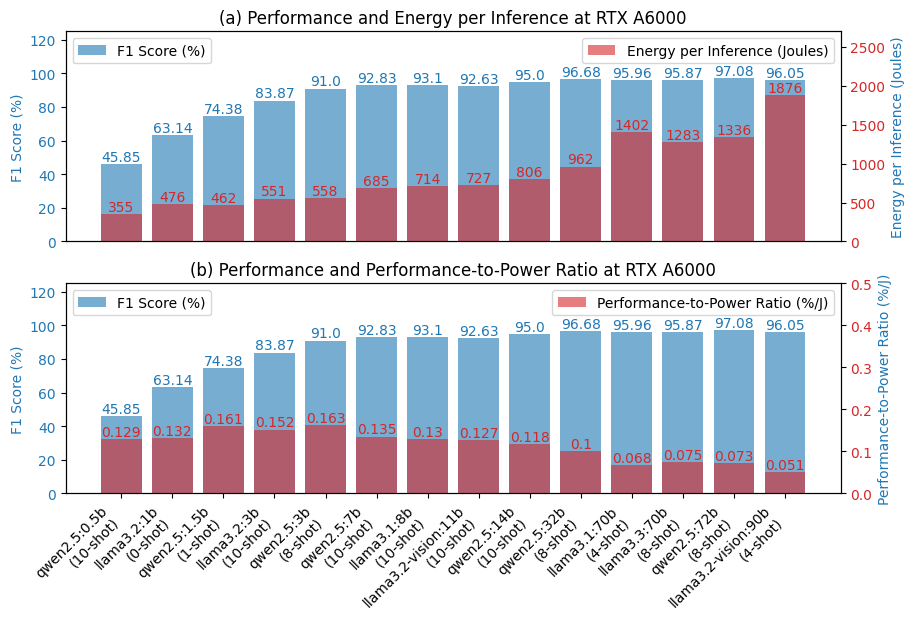
\includegraphics[width=\textwidth]{images/RTX-A6000-Perf-to-Power.png}
    \caption{Performance and Energy Efficiency Metrics on RTX A6000. (a) F1 Score (\%) vs. Energy per Inference (Joules). (b) F1 Score (\%) vs. Performance-to-Power Ratio (\%/J). Large models achieve high F1 scores but consume significantly more energy, while small models offer superior energy efficiency with acceptable performance trade-offs.}
    \label{fig:energy_efficiency}
\end{figure*}

Key findings from our comprehensive edge deployment evaluation:

\begin{enumerate}[leftmargin=*]
    \item \textbf{Quantization effectiveness:} Ollama's Q4\_K\_M quantization outperforms bitsandbytes 4-bit implementation, with llama3.1:8b achieving a mean F1 score of 92.87\% ($\pm$0.46\%) compared to its baseline of 89.50\% (3.37 percentage point improvement), and llama3.1:70b improving to 95.73\% ($\pm$0.23\%) from 95.51\% (0.22 percentage point improvement). This finding reinforces the open-source viability theme established in Chapter~\ref{ch:rag}, demonstrating that optimization techniques can unlock competitive performance from smaller models.
    
    \item \textbf{WSL performance gains:} Windows Subsystem for Linux (WSL) delivers substantial throughput improvements over native Windows. On RTX A6000, qwen2.5:0.5b processes 16,933 tokens/s on WSL compared to 816 tokens/s on Windows---a 21$\times$ speedup. This gap narrows for larger models, with differences as low as 15\% at 90B parameters.
    
    \item \textbf{Optimal model sizing:} Medium-sized models (7B--32B) achieve the best balance between performance and efficiency:
    \begin{itemize}
        \item qwen2.5:32b attains 96.75\% ($\pm$0.11\%) F1 score with practical inference speeds (mean 710 t/s across platforms)
        \item qwen2.5:7b achieves 92.64\% ($\pm$0.14\%) F1 with mean throughput of 2,873 t/s
        \item llama3.1:8b reaches 92.87\% ($\pm$0.46\%) F1 with mean throughput of 3,017 t/s
    \end{itemize}
    
    \item \textbf{Cross-platform stability:} Larger models exhibit increased cross-platform consistency, with F1 score standard deviations narrowing from 0.26--0.90\% (small models) to 0.07--0.23\% (large models), indicating more robust quantization at scale.
    
    \item \textbf{Energy trade-offs:} Large models such as qwen2.5:72b and llama3.2-vision:90b achieve high F1 scores (97.08\% and 96.05\%) but consume 1,283--1,876 Joules per inference. Small models like llama3.2-3b and qwen2.5:3b consume only 551--558 Joules while achieving 83.87\% and 91.00\% F1 respectively. Small models like qwen2.5:1.5b and qwen2.5:3b achieve the highest performance-to-power ratios (0.161 and 0.163 \%/J), ideal for energy-efficient deployments.
\end{enumerate}

Tables~\ref{tab:edge_results_small}, \ref{tab:edge_results_medium}, and \ref{tab:edge_results_large} summarize performance across hardware platforms by model category.

\begin{table}[htbp]
\centering
\caption{Edge Deployment Performance: Small Models (0.5B--3B)}
\label{tab:edge_results_small}
\resizebox{\textwidth}{!}{%
\begin{tabular}{@{}lcccc@{}}
\toprule
\textbf{Model} & \textbf{Mean F1 (\%)} & \textbf{Std (\%)} & \textbf{Mean T-put (t/s)} & \textbf{Mean Time (s)} \\
\midrule
qwen2.5:0.5b & 46.66 & 0.77 & 7,141 & 0.942 \\
llama3.2:1b & 63.17 & 0.33 & 2,033 & 1.357 \\
qwen2.5:1.5b & 74.21 & 0.90 & 3,479 & 1.038 \\
llama3.2:3b & 83.97 & 0.32 & 4,400 & 1.328 \\
qwen2.5:3b & 90.89 & 0.26 & 3,833 & 1.346 \\
\bottomrule
\end{tabular}
}
\end{table}

\begin{table}[htbp]
\centering
\caption{Edge Deployment Performance: Medium Models (7B--32B)}
\label{tab:edge_results_medium}
\resizebox{\textwidth}{!}{%
\begin{tabular}{@{}lcccc@{}}
\toprule
\textbf{Model} & \textbf{Mean F1 (\%)} & \textbf{Std (\%)} & \textbf{Mean T-put (t/s)} & \textbf{Mean Time (s)} \\
\midrule
qwen2.5:7b & 92.64 & 0.14 & 2,873 & 1.840 \\
llama3.1:8b & 92.87 & 0.46 & 3,017 & 1.785 \\
llama3.2-vision:11b & 92.89 & 0.33 & 2,950 & 1.746 \\
qwen2.5:14b & 95.00 & 0.14 & 1,629 & 3.004 \\
qwen2.5:32b & 96.75 & 0.11 & 710 & 7.781 \\
\bottomrule
\end{tabular}
}
\end{table}

\begin{table}[htbp]
\centering
\caption{Edge Deployment Performance: Large Models (70B--90B)}
\label{tab:edge_results_large}
\resizebox{\textwidth}{!}{%
\begin{tabular}{@{}lcccc@{}}
\toprule
\textbf{Model} & \textbf{Mean F1 (\%)} & \textbf{Std (\%)} & \textbf{Mean T-put (t/s)} & \textbf{Mean Time (s)} \\
\midrule
llama3.1:70b & 95.73 & 0.23 & 287 & 8.762 \\
llama3.3:70b & 95.84 & 0.07 & 368 & 16.513 \\
qwen2.5:72b & 96.90 & 0.20 & 263 & 10.660 \\
llama3.2-vision:90b & 96.04 & 0.07 & 90 & 17.739 \\
\bottomrule
\end{tabular}
}
\end{table}

\subsection{Deploying Reasoning LLMs on Consumer Hardware}
\label{subsec:reasoning_deployment}

\subsubsection{Motivation}

Deploying reasoning-enabled LLMs for sentiment analysis requires balancing accuracy, explainability, and efficiency under consumer hardware constraints. We present a cross-architecture evaluation of three reasoning model families---DeepSeek-R1, Qwen3, and GPT-OSS---spanning 17 open-weight variants. This addresses a critical gap: most existing evaluations target datacenter or cloud settings, leaving practitioners without evidence-based guidelines for consumer hardware deployment.

\subsubsection{Reasoning Intensity Metric}

We introduce Reasoning Intensity (RI) to capture trade-offs between explanation depth and computational cost:

\begin{equation}
RI = \frac{\text{Mean Reasoning Tokens (MRT)}}{\text{Mean Reasoning Tokens (MRT)} + \text{Mean Output Tokens (MOT)}}
\end{equation}

For DeepSeek-R1 models, both the \textit{reasoning content} (step-by-step thought process) and the final JSON output are included in the token count. The reasoning content refers to the complete trace of the model's thought process generated during inference, including intermediate evaluations and decision-making steps. This metric enables systematic comparison of reasoning strategies across architectures and complements the evaluation framework established in earlier chapters by capturing a dimension---reasoning overhead---not addressed by traditional accuracy metrics.

\subsubsection{Experimental Setup}

We evaluate models on fine-grained Amazon Reviews sentiment classification (5 classes: Strongly Negative, Negative, Neutral, Positive, Strongly Positive) using few-shot prompting. The primary benchmark comprises 1,838 reviews with human annotation, split 70\%/30\% for training/testing. To assess temporal robustness, we introduce Testset2: 574 manually annotated contemporary Amazon reviews collected in mid-2025.

\textbf{Model Families:}
\begin{itemize}[leftmargin=*]
    \item \textbf{DeepSeek-R1:} 8B, 14B, 32B, and 70B variants
    \item \textbf{Qwen3:} 0.6B, 1.7B, 4B, 8B, 14B, 30B, and 32B variants
    \item \textbf{GPT-OSS:} 20B and 120B, each with low/medium/high reasoning configurations
\end{itemize}

All models were executed via Ollama v0.11.4 using 4-bit quantization (MXFP4 for GPT-OSS; Q4\_K\_M for others), with a context length of 8,192 tokens.

\subsubsection{Results}

Table~\ref{tab:reasoning_deployment} presents deployment performance across model families on NVIDIA H100 GPU (96GB VRAM).

\begin{table}[htbp]
\centering
\caption{Cross-Architecture Reasoning Performance (5-Level Sentiment) on H100 GPU}
\label{tab:reasoning_deployment}
\resizebox{\textwidth}{!}{%
\begin{tabular}{@{}lccccccc@{}}
\toprule
\textbf{Model} & \textbf{F1 (\%)} & \textbf{Acc (\%)} & \textbf{MRT} & \textbf{MOT} & \textbf{RI} & \textbf{VRAM} & \textbf{Time (s)} \\
\midrule
\multicolumn{8}{c}{\textit{DeepSeek-R1 Family}} \\
\midrule
deepseek-r1:8b & 71.0 & 68.8 & 338 & 49 & 0.873 & 13 GB & 3.71 \\
deepseek-r1:14b & 77.4 & 75.5 & 248 & 54 & 0.819 & 18 GB & 4.88 \\
deepseek-r1:32b & \textbf{81.7} & \textbf{79.9} & 241 & 34 & 0.873 & 31 GB & 7.05 \\
deepseek-r1:70b & 74.2 & 71.3 & 237 & 40 & 0.855 & 58 GB & 12.08 \\
\midrule
\multicolumn{8}{c}{\textit{Qwen3 Family}} \\
\midrule
qwen3:0.6b & 65.2 & 64.8 & 236 & 72 & 0.765 & 6.1 GB & 1.34 \\
qwen3:1.7b & 75.7 & 76.8 & 217 & 57 & 0.790 & 6.8 GB & 1.56 \\
qwen3:4b & 84.3 & 83.7 & 284 & 60 & 0.825 & 11 GB & 3.93 \\
qwen3:8b & \textbf{84.8} & \textbf{84.9} & 249 & 59 & 0.807 & 13 GB & 8.35 \\
qwen3:14b & 84.6 & 83.7 & 245 & 61 & 0.799 & 19 GB & 10.20 \\
qwen3:30b & 84.3 & 84.8 & 1234 & 20 & 0.984 & 26 GB & 12.35 \\
qwen3:32b & 82.3 & 81.3 & 279 & 60 & 0.821 & 40 GB & 15.71 \\
\midrule
\multicolumn{8}{c}{\textit{GPT-OSS Family}} \\
\midrule
gpt-oss:20b (low) & 66.9 & 64.2 & 13 & 18 & 0.417 & 23 GB & 0.64 \\
gpt-oss:20b (medium) & 81.7 & 81.3 & 165 & 28 & 0.851 & 23 GB & 2.30 \\
gpt-oss:20b (high) & 84.6 & 83.8 & 744 & 30 & 0.961 & 23 GB & 8.60 \\
gpt-oss:120b (low) & 85.5 & 85.3 & 22 & 40 & 0.361 & 81 GB & 1.58 \\
gpt-oss:120b (medium) & \textbf{86.2} & \textbf{86.4} & 115 & 42 & 0.728 & 81 GB & 3.15 \\
gpt-oss:120b (high) & 83.4 & 82.8 & 679 & 43 & 0.940 & 81 GB & 11.84 \\
\bottomrule
\end{tabular}
}
\end{table}

Key findings reveal three distinct reasoning regimes:

\begin{enumerate}[leftmargin=*]
    \item \textbf{Best accuracy:} GPT-OSS achieves the highest F1 (86.2\% with gpt-oss:120b medium configuration) but requires 81 GB VRAM, far exceeding consumer GPU limits.
    
    \item \textbf{Practical balance:} Qwen3 delivers the most practical balance for consumer deployment. Within the 16GB VRAM constraint of an RTX 4090 Laptop, three models are viable:
    \begin{itemize}
        \item qwen3:8b: Optimal accuracy (84.8\% F1), 13GB VRAM, 8.35s inference
        \item qwen3:4b: Balanced performance (84.3\% F1), 11GB VRAM, 3.93s inference
        \item qwen3:1.7b: Resource-constrained option (75.7\% F1), 6.8GB VRAM, 1.56s inference
    \end{itemize}
    
    \item \textbf{Reasoning intensity patterns:} The results reveal three operational regimes:
    \begin{itemize}
        \item \textit{Minimal Reasoning} (RI $<$ 0.5): GPT-OSS low configurations prioritize throughput over explainability
        \item \textit{Balanced Reasoning} (0.5 $\leq$ RI $\leq$ 0.85): Most top-performing models operate here, including gpt-oss:120b (medium) achieving 86.2\% F1 with RI = 0.728
        \item \textit{Intensive Reasoning} (RI $>$ 0.85): DeepSeek-R1 models allocate 85--98\% of tokens to reasoning, enhancing explainability with modest accuracy gains
    \end{itemize}
    
    \item \textbf{Architecture over scale:} Larger models do not always outperform smaller counterparts. deepseek-r1:32b (81.7\% F1) substantially outperforms deepseek-r1:70b (74.2\% F1), demonstrating that architectural efficiency matters more than parameter count. This finding echoes the Orca-2-13b results from Chapter~\ref{ch:rag}, reinforcing the dissertation's broader finding that model optimization often matters more than scale.
\end{enumerate}

\subsubsection{Temporal Robustness Evaluation}

To assess model robustness under temporal drift, we evaluate on Testset2 comprising 574 manually annotated contemporary reviews from mid-2025.

\begin{table}[htbp]
\centering
\caption{Cross-Platform Temporal Robustness: Original vs. Contemporary Reviews}
\label{tab:temporal_robustness}
\resizebox{\textwidth}{!}{%
\begin{tabular}{@{}llcccc@{}}
\toprule
\textbf{Model} & \textbf{Hardware} & \textbf{Original F1 (\%)} & \textbf{Testset2 F1 (\%)} & \textbf{$\Delta$ F1} & \textbf{RI Stability} \\
\midrule
qwen3:1.7b & H100 & 75.7 & 57.9 & -17.8 & $\pm$0.012 \\
qwen3:1.7b & RTX 4090 & 72.6 & 58.1 & -14.5 & $\pm$0.010 \\
qwen3:4b & H100 & 84.3 & 67.8 & -16.5 & $\pm$0.011 \\
qwen3:4b & RTX 4090 & 81.7 & 65.7 & -16.0 & $\pm$0.001 \\
qwen3:8b & H100 & 84.8 & 72.3 & -12.5 & $\pm$0.021 \\
qwen3:8b & RTX 4090 & 82.1 & 73.3 & -8.8 & $\pm$0.017 \\
\bottomrule
\end{tabular}
}
\end{table}

Results reveal consistent 10--17 percentage point F1 degradation across models on contemporary data, though reasoning intensity remains remarkably stable ($\pm$0.02) across temporal domains. Notably, qwen3:8b exhibits superior temporal resilience, maintaining the smallest relative degradation among evaluated models. This suggests that while models' reasoning processes are robust, their learned sentiment patterns require periodic updating to account for evolving language use and product categories.

\section{Reasoning Enhancement Techniques}
\label{sec:reasoning_enhancement}

\subsection{Logical Reasoning via Lateral Thinking Puzzles}
\label{subsec:turtle_soup}

\subsubsection{The Turtle Soup Benchmark}

To assess logical reasoning capabilities, we utilize the Turtle Soup Question Answering (TSQA) dataset from the ``Logical Reasoning with LLM'' competition. The Turtle Soup game, popularized by the book \textit{Challenging Lateral Thinking Puzzles}, presents mystery puzzles requiring lateral thinking---players must deduce hidden rationales through yes/no questions. The game's name originates from a classic problem: a man orders turtle soup at a restaurant and subsequently commits suicide; players must deduce the rationale through constrained questioning.

The dataset comprises:
\begin{itemize}[leftmargin=*]
    \item 25,000 labeled training questions
    \item 3,000 labeled validation questions
    \item Chinese language content (adding complexity for primarily English-trained models)
\end{itemize}

Model responses are constrained to five categories: 是 (Yes), 不是 (No), 不重要 (Unimportant), 问法错误 (Wrong Question), and 回答正确 (Correct Answer).

\subsubsection{Methodology}

\textbf{Model Selection:} We evaluate diverse state-of-the-art LLMs including GPT-4o, o1-preview, o1-mini, Qwen2.5 (3B--72B), Llama3.1 (8B--70B), InternLM2.5 (7B, 7B-1M, 20B), and Mistral-7B. For open-source models lacking native Chinese support, we utilized their fine-tuned Chinese versions.

\textbf{Few-shot Prompting:} We employ a concise system prompt (``You are an expert in logical reasoning'') with representative examples covering all answer categories. Few-shot configurations range from 0 to 50 shots.

\textbf{Parameter-Efficient Fine-Tuning:} We apply LoRA~\cite{hu2022lora} (rank 64, alpha 128) and QLoRA~\cite{dettmers2023qlora} (4-bit quantization) for efficient adaptation on consumer-grade hardware. This approach aligns with the parameter-efficient techniques that enabled the multi-agent systems in Chapter~\ref{ch:agentic} to run on edge hardware.

\subsubsection{Valid Classification Ratio (VCR)}

We introduce the Valid Classification Ratio (VCR) as a novel metric for assessing output reliability:

\begin{equation}
VCR = \frac{\text{Number of valid classifications}}{\text{Total number of outputs}}
\end{equation}

VCR measures the proportion of responses that map to valid answer categories, capturing model reliability beyond accuracy. During evaluation, we observed that some models produce outputs containing extraneous text or failing to match predefined labels, necessitating post-processing before F1 calculation. This metric complements the Agentic Success Rate (ASR) introduced in Chapter~\ref{ch:agentic}, but focuses specifically on output validity rather than tool-calling reliability. While ASR measures whether agents successfully execute multi-step workflows, VCR measures whether models produce outputs conforming to expected formats---a prerequisite for downstream processing in production systems.

\subsubsection{Results}

Table~\ref{tab:reasoning_results} presents logical reasoning performance across few-shot and fine-tuned configurations.

\begin{table}[htbp]
\centering
\caption{Logical Reasoning Performance on TSQA Benchmark}
\label{tab:reasoning_results}
\begin{tabular}{@{}llccccc@{}}
\toprule
\textbf{Model} & \textbf{Method} & \textbf{Shots} & \textbf{Acc (\%)} & \textbf{F1 (\%)} & \textbf{VCR (\%)} \\
\midrule
GPT-4o & Few-shot & 10 & 79.12 & 80.36 & 99.2 \\
o1-preview & Few-shot & 50 & 75.89 & 77.08 & 98.7 \\
o1-mini & Few-shot & 50 & 74.56 & 75.89 & 98.4 \\
Qwen2.5-72B & Few-shot & 10 & 79.85 & \textbf{80.88} & 98.5 \\
Qwen2.5-7B & Few-shot & 50 & 74.23 & 75.45 & 97.8 \\
Qwen2.5-3B & Few-shot & 50 & 71.34 & 72.67 & 96.9 \\
Llama3.1-70B & Few-shot & 20 & 76.89 & 78.12 & 98.1 \\
Llama3.1-8B & Few-shot & 50 & 73.45 & 74.78 & 97.5 \\
InternLM2.5-7B-1M & Few-shot & 50 & 75.67 & 77.01 & 97.9 \\
InternLM2.5-7B & Few-shot & 50 & 74.12 & 75.34 & 97.6 \\
Mistral-7B & Few-shot & 50 & 72.89 & 74.12 & 97.2 \\
\midrule
Llama3.1-70B & Fine-tuned & -- & 79.65 & \textbf{80.77} & 99.1 \\
Qwen2-72B & Fine-tuned & -- & 79.21 & 80.33 & 99.0 \\
InternLM2.5-7B-1M & Fine-tuned & -- & 78.92 & 80.28 & 98.8 \\
InternLM2.5-20B & Fine-tuned & -- & 78.89 & 80.28 & 98.9 \\
InternLM2.5-7B & Fine-tuned & -- & 78.45 & 79.89 & 98.7 \\
Qwen2.5-7B & Fine-tuned & -- & 77.89 & 79.23 & 98.6 \\
\bottomrule
\end{tabular}
\end{table}

Key findings:

\begin{enumerate}[leftmargin=*]
    \item \textbf{Open-source competitiveness:} Qwen2.5-72B achieved the highest few-shot F1 score (80.88\%), surpassing GPT-4o's 80.36\% with only 10-shot prompting, demonstrating that open-source models can match or exceed proprietary alternatives on complex reasoning tasks. This reinforces the open-source viability findings from Chapter~\ref{ch:rag} where Orca-2-13b achieved comparable performance to GPT-4 in RAG applications.
    
    \item \textbf{Unexpected o1-preview performance:} The o1-preview model, despite its purported superior reasoning capabilities, exhibited lower F1 scores (77.08\%) compared to GPT-4o even with 50-shot prompting. This warrants further investigation into whether o1-preview's reasoning strengths are better suited to other task types.
    
    \item \textbf{Fine-tuning superiority:} Fine-tuning generally yields superior results, with Llama3.1-70B achieving 80.77\% F1 after fine-tuning---surpassing all few-shot configurations except Qwen2.5-72B.
    
    \item \textbf{Extended context benefit:} InternLM2.5-7B-1M, with its 1-million-token context window, demonstrated significant improvement from few-shot (77.01\%) to fine-tuned (80.28\%), ranking third overall among fine-tuned models despite its smaller parameter count.
    
    \item \textbf{VCR improvements:} Fine-tuning substantially improves VCR, with all fine-tuned models exceeding 98.6\% valid classification rates compared to 96.9--99.2\% for few-shot configurations. Notably, Mistral-7B showed extremely low VCR values (ranging from 1.17\% to 14.20\%) in few-shot settings, but fine-tuning improved VCR to 100\% within just 0.2 epochs, demonstrating the dramatic reliability improvements achievable through targeted optimization.
\end{enumerate}

\subsubsection{Fine-Tuning Analysis}

We observed that training beyond 1 epoch often leads to overfitting. To address this, we implemented early stopping with 0.2 epoch granularity and selected optimal checkpoints based on validation performance. For instance, Qwen2-72B achieved peak F1 (80.33\%) at 0.8 epochs, while smaller models typically required 0.8--1.0 epochs. Larger models consistently peaked earlier (2--3 epochs) than smaller ones (4--5 epochs), suggesting that larger models learn task-specific patterns more efficiently but are also more prone to overfitting.

\subsection{Explainable Sentiment Analysis with DeepSeek-R1}
\label{subsec:deepseek_sentiment}

\subsubsection{Motivation}

Large language models have transformed sentiment analysis, yet balancing accuracy, efficiency, and explainability remains a critical challenge. DeepSeek-R1, an open-source reasoning model trained via reinforcement learning, introduces a novel approach by generating step-by-step reasoning processes during inference. This distinguishes it from conventional LLMs that prioritize direct responses, offering native interpretability without external explanation mechanisms.

\subsubsection{Experimental Setup}

We evaluate DeepSeek-R1 (full 671B model and distilled variants: 8B, 14B, 32B, 70B) against GPT-4o and GPT-4o-mini on three affective computing tasks:

\begin{itemize}[leftmargin=*]
    \item \textbf{Amazon Reviews:} 5-class sentiment classification (Strongly Negative to Strongly Positive), 1,838 human-annotated reviews
    \item \textbf{IMDB Movie Reviews:} Binary classification (Negative/Positive)
    \item \textbf{GoEmotions:} 27-class emotion recognition for nuanced sentiment evaluation
\end{itemize}

We employ few-shot prompting (0-shot to 50-shot configurations) to assess in-context learning effectiveness.

\subsubsection{Results}

Table~\ref{tab:deepseek_sentiment} presents sentiment analysis performance across tasks.

\begin{table}[htbp]
\centering
\caption{DeepSeek-R1 Performance on Sentiment Classification Tasks}
\label{tab:deepseek_sentiment}
\begin{tabular}{@{}lcccccc@{}}
\toprule
\textbf{Model} & \textbf{Task} & \textbf{Acc (\%)} & \textbf{F1 (\%)} & \textbf{Shots} & \textbf{T-put (t/s)} \\
\midrule
\multicolumn{6}{c}{\textit{Amazon Reviews (5-class)}} \\
\midrule
DeepSeek-R1 (671B) & 5-class & 91.29 & \textbf{91.39} & 30 & 334 \\
GPT-4o & 5-class & 86.57 & 87.99 & 40 & 1,220 \\
GPT-4o-mini & 5-class & 81.31 & 83.02 & 50 & 2,124 \\
deepseek-r1:32b & 5-class & 79.85 & 80.89 & 50 & 254 \\
deepseek-r1:14b & 5-class & 78.23 & 79.06 & 30 & 414 \\
deepseek-r1:8b & 5-class & 76.77 & 78.31 & 40 & 520 \\
\midrule
\multicolumn{6}{c}{\textit{IMDB Binary Sentiment}} \\
\midrule
DeepSeek-R1 (671B) & Binary & 99.12 & \textbf{99.31} & 5 & 334 \\
GPT-4o & Binary & 97.23 & 97.47 & 20 & 1,220 \\
deepseek-r1:70b & Binary & 97.89 & 98.04 & 20 & 52 \\
deepseek-r1:32b & Binary & 95.73 & 95.75 & 10 & 254 \\
\midrule
\multicolumn{6}{c}{\textit{GoEmotions (27-class)}} \\
\midrule
DeepSeek-R1 (671B) & 27-class & 45.33 & 46.02 & 10 & 48 \\
GPT-4o & 27-class & 45.17 & 45.99 & 10 & 424 \\
deepseek-r1:70b & 27-class & 44.00 & 44.57 & 10 & 52 \\
\bottomrule
\end{tabular}
\end{table}

Key findings:

\begin{enumerate}[leftmargin=*]
    \item \textbf{Superior few-shot efficiency:} DeepSeek-R1 achieves 91.39\% F1 on 5-class sentiment with just 30 shots, representing an approximately eightfold improvement in few-shot efficiency over GPT-4o (which requires 40 shots for 87.99\% F1). This demonstrates that reasoning-native architectures can achieve strong performance with fewer examples.
    
    \item \textbf{Binary task excellence:} On IMDB binary classification, DeepSeek-R1 achieves 99.31\% accuracy with only 5 shots, demonstrating exceptional performance on simpler tasks with minimal prompting.
    
    \item \textbf{Architecture-specific distillation effects:} The 32B Qwen2.5-based distilled model outperforms the 70B Llama-based variant by 6.69 percentage points on Amazon Reviews (80.89\% vs. 74.20\%), suggesting that distillation quality depends more on base architecture compatibility than parameter count.
    
    \item \textbf{Throughput trade-off:} DeepSeek-R1's reasoning process reduces throughput (334 t/s at peak) compared to GPT-4o (1,220 t/s), but offers superior explainability via transparent reasoning traces. This trade-off is acceptable for applications requiring auditability.
\end{enumerate}

\subsubsection{Explainability Analysis}

DeepSeek-R1's reasoning traces demonstrate sophisticated analysis patterns that enhance transparency:

\begin{itemize}[leftmargin=*]
    \item \textbf{Resolution of mixed experiences:} Both DeepSeek-R1 and GPT-4o correctly identify neutral sentiment in mixed reviews, but follow distinct reasoning paths. GPT-4o balances product failure against positive customer service in a single-layer explanation, while DeepSeek-R1 traces temporal progression from negative experience to resolution, providing dual-layer explanation with both a brief prompt-compliant summary and extensive step-by-step reasoning.
    
    \item \textbf{Emotional vs. functional analysis:} DeepSeek-R1 assigns greater weight to emotional impact (e.g., feeling ``duped''), leading to different classifications than GPT-4o's focus on functional benefits. This heightened sensitivity to emotional language enables more nuanced sentiment detection.
    
    \item \textbf{Treatment of indirect experiences:} GPT-4o interprets widespread user complaints as indicative of negative sentiment even without direct personal experience, while DeepSeek-R1 classifies such reviews as ``Neutral'' since they focus on reporting issues rather than expressing direct dissatisfaction.
\end{itemize}

The key stylistic difference is that DeepSeek-R1 generates an \textit{intrinsic reasoning trace}---not prompted, but inherent to its architecture---representing a unique form of built-in explainability that emerges naturally from reinforcement learning training.

\subsection{Task Complexity and Reasoning Effectiveness}
\label{subsec:task_complexity}

\subsubsection{Motivation}

Building on the initial investigation of DeepSeek-R1 in Section~\ref{subsec:deepseek_sentiment}, we significantly extend the scope to address a central question: \textit{Do reasoning capabilities justify their computational overhead for sentiment tasks of varying complexity?} Where Section~\ref{subsec:deepseek_sentiment} established DeepSeek-R1's superior few-shot efficiency (approximately 8$\times$ over GPT-4o), this section investigates whether such advantages generalize across task complexities and model architectures.

While reasoning-enhanced LLMs have demonstrated strong performance on mathematical and logical tasks, the effectiveness of reasoning mechanisms for foundational NLP applications such as sentiment analysis remains largely untested. Recent work in financial sentiment analysis provides early evidence of a potential mismatch, demonstrating that chain-of-thought reasoning leads to ``overthinking'' and degraded performance compared to intuitive classification~\cite{li2025financial}. This suggests a task-complexity hypothesis: simple classification tasks with clear categorical boundaries may require different cognitive strategies than complex tasks with nuanced distinctions.

\subsubsection{Experimental Setup}

We conduct the first large-scale, cross-architectural comparison of reasoning versus non-reasoning modes across sentiment analysis tasks of varying complexity. The evaluation spans 504 unique configurations (7 model families $\times$ 3 datasets $\times$ 7 shot levels $\times$ thinking/non-thinking variants):

\textbf{Model Families:}
\begin{itemize}[leftmargin=*]
    \item \textbf{DeepSeek-R1 Series:} Full 671B model and distilled variants (8B, 14B, 32B, 70B), compared against base models DeepSeek-V3, LLaMA (3.1-8B, 3.3-70B), and Qwen2.5 (14B, 32B)
    \item \textbf{Qwen3:} Dense models (4B, 8B, 14B, 32B) supporting both thinking (T) and non-thinking (N) modes with adaptive ``thinking budgets''
    \item \textbf{Granite3.3:} Lightweight models (2B, 8B) with conditional reasoning in T and N modes
    \item \textbf{Magistral:} 24B model with RL-based reasoning in T and N modes
\end{itemize}

\textbf{Datasets Spanning Complexity Levels:}
\begin{itemize}[leftmargin=*]
    \item \textbf{IMDB Movie Reviews:} Binary sentiment (positive/negative), representing simple classification
    \item \textbf{Amazon Reviews:} Five-class sentiment (strongly negative to strongly positive), representing moderate complexity
    \item \textbf{GoEmotions:} 27 emotion categories, representing high complexity
\end{itemize}

Models were evaluated under 0--5--10--20--30--40--50-shot settings, with stratified sampling for few-shot exemplars.

\subsubsection{Results: Distilled vs. Base Model Performance}

Table~\ref{tab:distillation_complexity} presents performance comparisons between reasoning-enhanced distilled models and their base counterparts.

\begin{table}[htbp]
\centering
\caption{Reasoning-Focused Distillation vs. Base Model Performance. Diff. indicates performance difference (Distilled $-$ Base). Failure Rate (FR) shows percentage of comparisons where distilled models underperform or match base models.}
\label{tab:distillation_complexity}
\resizebox{\textwidth}{!}{%
\begin{tabular}{@{}llcccccc@{}}
\toprule
\textbf{Dataset} & \textbf{Model Pair} & \textbf{Base 0S} & \textbf{Dist. 0S} & \textbf{Diff. 0S} & \textbf{Diff. BS} & \textbf{FR (\%)} \\
\midrule
\multirow{3}{*}{IMDB} & DSV3 vs DSR1 & 97.9 & 78.0 & \textcolor{red}{-19.9} & \textcolor{red}{-0.0} & \multirow{3}{*}{\textcolor{red}{100}} \\
& Llama3.3-70B vs DSR1-70B & 98.0 & 97.1 & \textcolor{red}{-0.9} & \textcolor{red}{-1.3} & \\
& Qwen2.5-32B vs DSR1-32B & 97.8 & 96.0 & \textcolor{red}{-1.8} & \textcolor{red}{-1.3} & \\
\midrule
\multirow{3}{*}{Amazon} & Llama3.3-70B vs DSR1-70B & 82.5 & 64.1 & \textcolor{red}{-18.4} & \textcolor{red}{-12.7} & \multirow{3}{*}{\textcolor{orange}{80}} \\
& Qwen2.5-14B vs DSR1-14B & 74.7 & 61.9 & \textcolor{red}{-12.8} & \textcolor{red}{-8.0} & \\
& Qwen2.5-32B vs DSR1-32B & 63.8 & 69.0 & \textcolor{blue}{+5.2} & \textcolor{red}{-3.9} & \\
\midrule
\multirow{3}{*}{GoEmotions} & DSV3 vs DSR1 & 39.1 & 42.8 & \textcolor{blue}{+3.7} & \textcolor{blue}{+3.8} & \multirow{3}{*}{\textcolor{blue}{50}} \\
& Llama3.3-70B vs DSR1-70B & 38.6 & 34.0 & \textcolor{red}{-4.6} & \textcolor{blue}{+4.8} & \\
& Qwen2.5-32B vs DSR1-32B & 34.0 & 34.7 & \textcolor{blue}{+0.7} & \textcolor{blue}{+3.2} & \\
\bottomrule
\end{tabular}
}
\end{table}

Key findings reveal systematic task-complexity patterns:

\begin{enumerate}[leftmargin=*]
    \item \textbf{Zero-shot degradation:} Distilled models underperform base models in zero-shot settings, with the largest drops on simple tasks: -19.9 pp (DSR1 vs. DSV3 on IMDB), -18.4 pp (DSR1-70B vs. Llama3.3-70B on Amazon). Mean degradation by dataset: -5.9 pp (IMDB), -7.6 pp (Amazon), -2.0 pp (GoEmotions).
    
    \item \textbf{Few-shot recovery:} Gaps narrow with examples---IMDB mean gap improves from -5.9 to -1.3 pp; Amazon from -7.6 to -5.2 pp. GoEmotions shows notable reversals where distilled models outperform bases (DSR1-70B: +4.8 pp, DSR1-32B: +3.2 pp).
    
    \item \textbf{Task-dependent failure rates:} IMDB shows 100\% failure rate (all 10 comparisons favor base models), Amazon shows 80\%, while GoEmotions shows 50\%---decreasing failure rates with increasing task complexity validate the hypothesis that reasoning becomes beneficial as classification granularity increases.
\end{enumerate}

\subsubsection{Results: Thinking vs. Non-Thinking Mode Analysis}

Table~\ref{tab:thinking_complexity} compares thinking and non-thinking modes across architectures with runtime-activated reasoning.

\begin{table}[htbp]
\centering
\caption{Thinking vs. Non-Thinking Mode Performance. Diff. = F1\_Thinking $-$ F1\_Non-thinking. Speed Ratio (SR) = Thinking latency / Non-thinking latency.}
\label{tab:thinking_complexity}
\resizebox{\textwidth}{!}{%
\begin{tabular}{@{}llcccccc@{}}
\toprule
\textbf{Dataset} & \textbf{Model} & \textbf{Non-think.} & \textbf{Thinking} & \textbf{Diff.} & \textbf{SR} & \textbf{FR (\%)} \\
\midrule
\multirow{4}{*}{IMDB} & Qwen3-4B & 98.2 & 98.4 & \textcolor{blue}{+0.2} & 5.5× & \multirow{4}{*}{\textcolor{orange}{36}} \\
& Qwen3-14B & 98.4 & 98.9 & \textcolor{blue}{+0.5} & 4.3× & \\
& Magistral-24B & 97.4 & 96.9 & \textcolor{red}{-0.5} & 9.7× & \\
& Granite3.3-8B & 98.3 & 96.0 & \textcolor{red}{-2.2} & 1.0× & \\
\midrule
\multirow{4}{*}{Amazon} & Qwen3-8B & 84.5 & 84.8 & \textcolor{blue}{+0.3} & 5.4× & \multirow{4}{*}{\textcolor{orange}{57}} \\
& Magistral-24B & 81.6 & 80.7 & \textcolor{red}{-0.9} & 14.4× & \\
& Qwen3-32B & 89.0 & 84.8 & \textcolor{red}{-6.8} & 11.5× & \\
& Granite3.3-2B & 74.1 & 63.9 & \textcolor{red}{-10.2} & 2.1× & \\
\midrule
\multirow{4}{*}{GoEmotions} & Magistral-24B & 35.0 & 43.7 & \textcolor{blue}{+8.8} & 54.4× & \multirow{4}{*}{\textcolor{blue}{14}} \\
& Qwen3-14B & 40.3 & 47.0 & \textcolor{blue}{+6.6} & 8.4× & \\
& Qwen3-32B & 39.8 & 45.9 & \textcolor{blue}{+6.2} & 7.4× & \\
& Qwen3-8B & 41.0 & 44.0 & \textcolor{blue}{+3.1} & 8.3× & \\
\bottomrule
\end{tabular}
}
\end{table}

Key findings across 42 zero-shot comparisons:

\begin{enumerate}[leftmargin=*]
    \item \textbf{Task-complexity dependence:} Thinking mode helps GoEmotions (86\% positive), shows mixed results on Amazon (43\% positive), and balanced effects on IMDB (64\% positive). Failure rates by dataset: Amazon 57\%, IMDB 36\%, GoEmotions 14\%---substantially lower failure rates for complex emotion recognition confirm reasoning mechanisms are most effective when task complexity justifies computational cost.
    
    \item \textbf{Few-shot convergence patterns:} Thinking advantages often diminish with examples. Magistral exhibits dramatic shifts: Amazon from +12.2 pp (zero-shot) to -0.9 pp (best-shot); IMDB from +2.1 pp to -0.5 pp. This suggests that on simpler tasks, examples provide sufficient guidance without reasoning overhead.
    
    \item \textbf{Efficiency trade-offs:} Speed ratios range from 1.0× to 54.4×, with highest overhead on GoEmotions (Magistral: 54.4×). Mean overhead across model families: Granite 1.0×--5.5×, Qwen3 2.5×--11.5×, Magistral 9.7×--54.4×.
\end{enumerate}

\subsubsection{Aggregate Performance Across Task Complexity}

Table~\ref{tab:aggregated_complexity} presents aggregated statistics across all 504 configurations, stratified by dataset and model type.

\begin{table}[htbp]
\centering
\caption{Aggregated Performance Statistics Across 504 Configurations. Statistics reported as mean $\pm$ std across 12 model pairs and 7 shot levels (0--50 shots).}
\label{tab:aggregated_complexity}
\begin{tabular}{@{}llccc@{}}
\toprule
\textbf{Dataset} & \textbf{Type} & \textbf{N} & \textbf{F1 (\%)} & \textbf{Diff. (\%)} \\
\midrule
\multirow{2}{*}{IMDB} & Base/Non-think. & 84 & $91.5 \pm 20.8$ & \multirow{2}{*}{\textcolor{red}{$-4.8\pm6.3$}} \\
& Dist./Think. & 84 & $86.7 \pm 25.7$ & \\
\midrule
\multirow{2}{*}{Amazon} & Base/Non-think. & 84 & $74.9 \pm 18.9$ & \multirow{2}{*}{\textcolor{red}{$-3.6\pm2.2$}} \\
& Dist./Think. & 84 & $71.3 \pm 17.7$ & \\
\midrule
\multirow{2}{*}{GoEmotions} & Base/Non-think. & 84 & $36.6 \pm 4.0$ & \multirow{2}{*}{\textcolor{blue}{$+2.0\pm1.0$}} \\
& Dist./Think. & 84 & $38.6 \pm 7.3$ & \\
\bottomrule
\end{tabular}
\end{table}

The decreasing performance gap with increasing task complexity---from -4.8 pp (binary) through -3.6 pp (5-class) to +2.0 pp (27-class)---validates the task-complexity hypothesis: reasoning mechanisms become more beneficial as classification granularity increases.

\subsubsection{Pareto Frontier Analysis}

Figure~\ref{fig:pareto_frontier} visualizes efficiency-performance trade-offs across all configurations. The Pareto frontier represents configurations where no alternative improves F1 without increasing latency, or reduces latency without sacrificing F1. This analysis extends the cost-effectiveness evaluation approach used for the LAJ framework in Chapter~\ref{ch:agentic}, applying similar principles to reasoning model selection.

\begin{figure}[t]
\centering
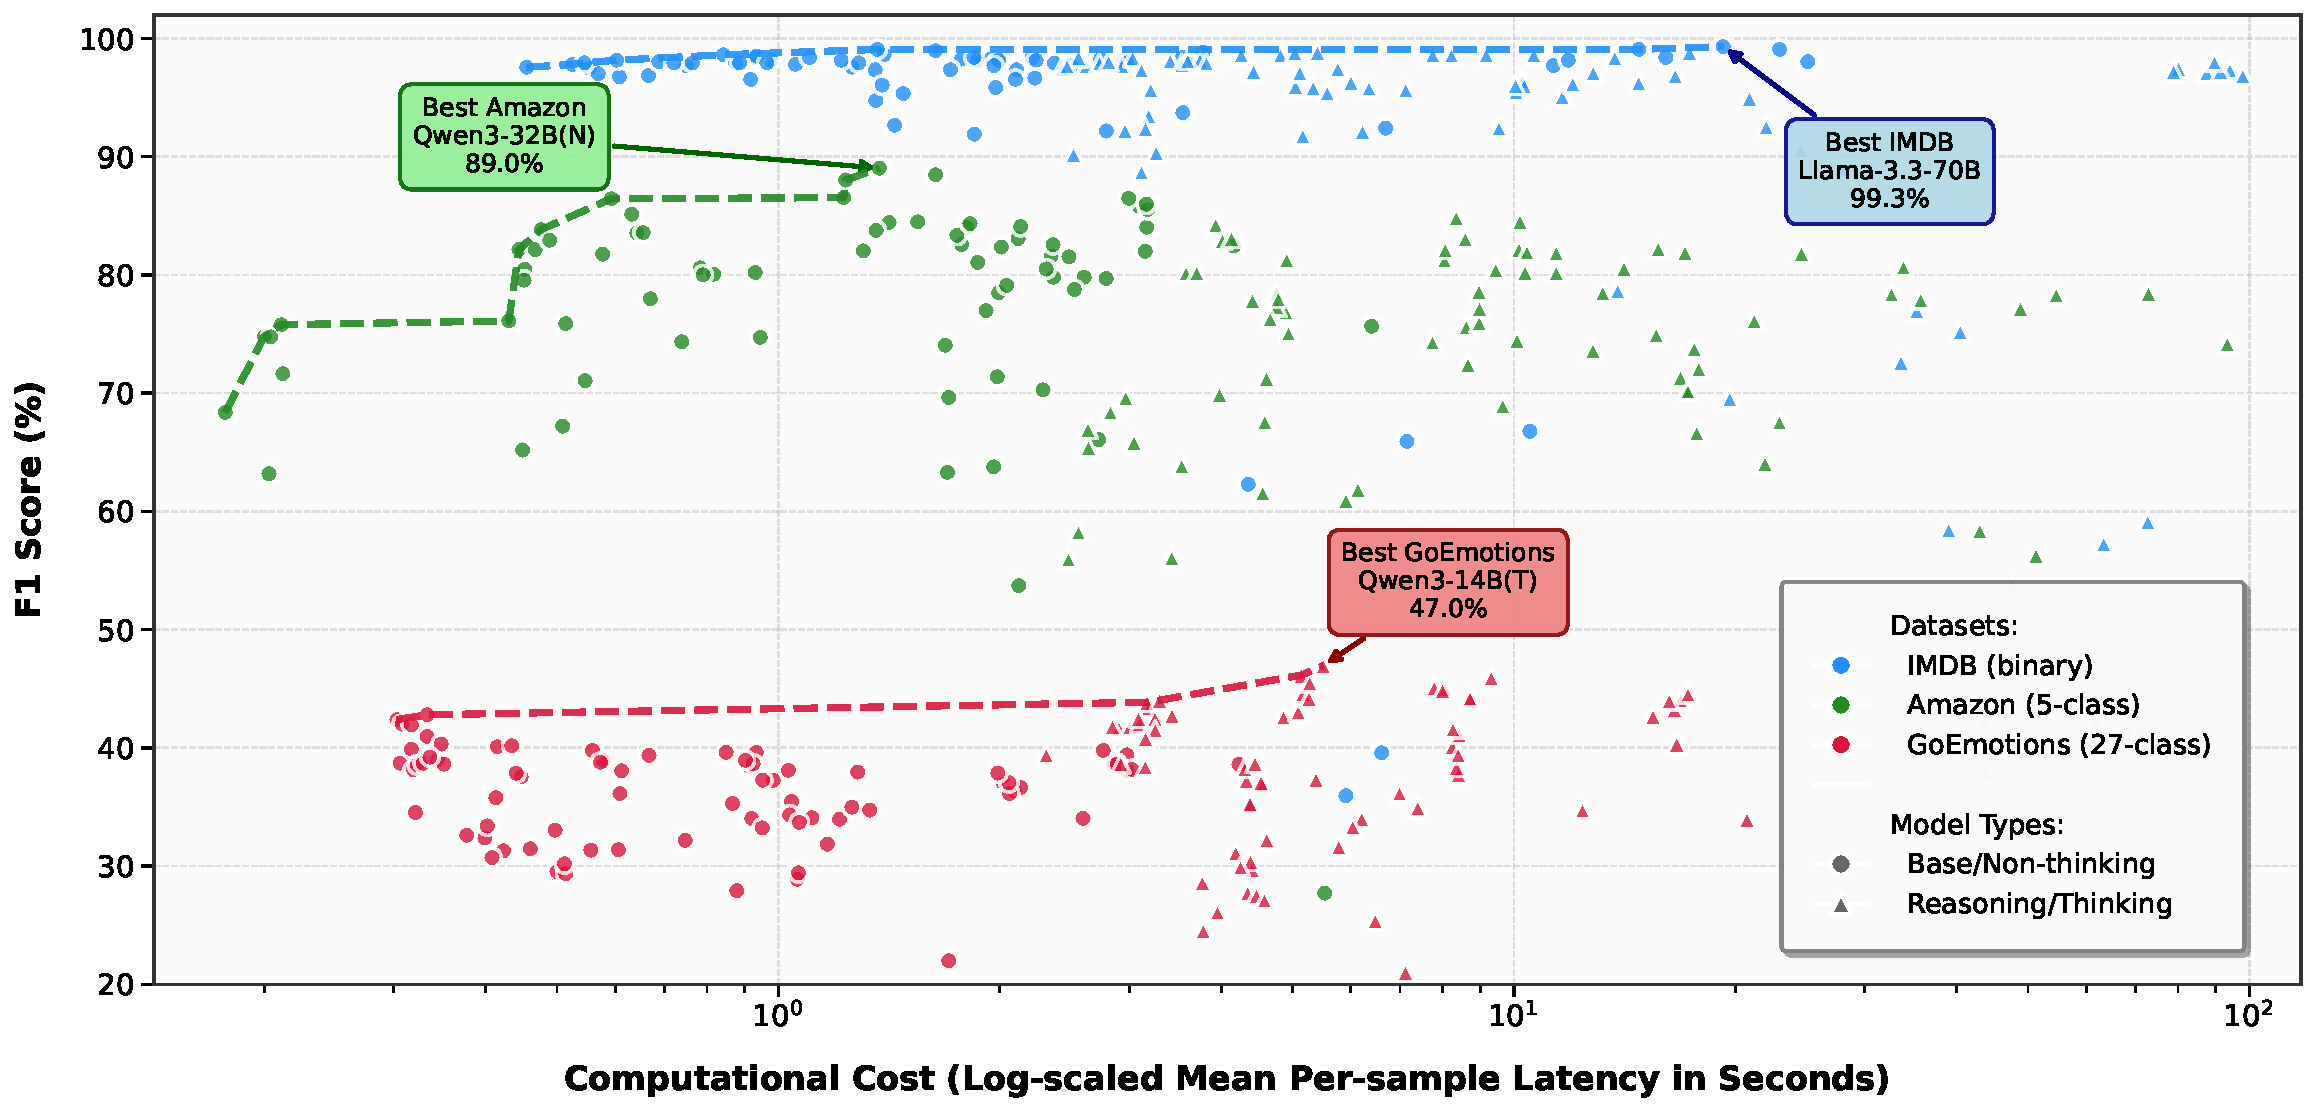
\includegraphics[width=\textwidth]{figures/pareto_frontier_v2.pdf}
\caption{Performance vs. computational cost. Circles: base/non-thinking; triangles: reasoning/thinking. Colors: IMDB (blue), Amazon (green), GoEmotions (red). Dashed lines: Pareto frontiers where no configuration dominates on both metrics. Evaluated on H100 via Ollama; DSR1/V3 excluded for consistency. Labels show top performers per dataset.}
\label{fig:pareto_frontier}
\end{figure}

Key observations from Pareto analysis:

\begin{enumerate}[leftmargin=*]
    \item \textbf{Task-dependent model representation:} IMDB frontier is dominated by base models achieving 97--99\% F1 with minimal latency. GoEmotions frontier includes reasoning models more frequently, justifying their overhead through accuracy gains.
    
    \item \textbf{Cost-performance curves:} IMDB shows flat frontier at high F1, indicating diminishing returns from additional compute. GoEmotions exhibits steeper slope, where latency increases yield greater accuracy improvements.
    
    \item \textbf{Practical guidance:} Base models dominate for most sentiment classification tasks. Reasoning should be reserved for complex emotion recognition where 2--4 pp improvements justify 2.1×--54× computational overhead.
\end{enumerate}

\subsubsection{Summary of Task Complexity Findings}

This comprehensive evaluation reveals that reasoning effectiveness in sentiment analysis is systematically task-dependent:

\begin{enumerate}[leftmargin=*]
    \item \textbf{Simple tasks (binary classification):} Base/non-thinking models provide superior performance (4.8 pp advantage) with lower computational overhead. Reasoning introduces noise rather than clarification.
    
    \item \textbf{Moderate tasks (5-class sentiment):} Mixed results with 3.6 pp average base model advantage. Reasoning can help disambiguate adjacent categories but may overcomplicate straightforward cases.
    
    \item \textbf{Complex tasks (27-class emotion):} Reasoning models achieve 2.0 pp advantage, with the lowest failure rate (14\%) among thinking vs. non-thinking comparisons. Extended reasoning helps navigate fine-grained distinctions between similar emotions.
    
    \item \textbf{Few-shot learning superiority:} Regardless of reasoning mode, few-shot learning yields improvements over zero-shot in the vast majority of cases, positioning it as a more robust strategy than reasoning activation for enhancing sentiment analysis performance.
\end{enumerate}

These findings provide principled deployment guidance: reserve reasoning for complex multi-class problems where accuracy gains justify computational overhead, and leverage few-shot learning for consistent improvements across all task complexities.

\section{Cross-Domain Applications}
\label{sec:cross_domain}

\subsection{Chinese-English Translation Optimization}
\label{subsec:translation}

\subsubsection{Motivation}

Machine translation between Chinese and English poses particular challenges due to significant differences in syntax, semantics, and morphology. Traditional approaches have struggled with complexities inherent in Chinese-English translation, particularly in handling idiomatic expressions, word order differences, and character-based text segmentation. We comprehensively evaluate LLMs across zero-shot, few-shot, and fine-tuned paradigms to establish best practices for practical deployment.

\subsubsection{Dataset}

We use the MAC (Manually Aligned Chinese-English) dataset\footnote{\url{https://github.com/bfsujason/mac}}, comprising parallel Mandarin-English texts from six Chinese novels representing diverse genres: humor, martial arts, classics, war, romance, and science fiction. After preprocessing to remove entries with missing content and splitting 80\%/20\%, the dataset contains 4,528 training and 1,133 testing sentence pairs.

\subsubsection{Evaluation Metrics}

\begin{enumerate}[leftmargin=*]
    \item \textbf{COMET-22:} Neural-based metric using contextual embeddings from pretrained language models. COMET-22 shows strong correlation with human judgments for Chinese-English translation, outperforming traditional metrics like BLEU and TER in alignment with human evaluations.
    
    \item \textbf{Translation Completeness Ratio (TCR):} During evaluation, we observed that some LLM outputs contained untranslated segments with Chinese characters. TCR measures the proportion of translations fully rendered into English:
    \begin{equation}
    TCR = \frac{\text{Number of complete translations}}{\text{Total number of entries}}
    \end{equation}
    where a ``complete translation'' is defined as one where no Chinese characters remain in the output text. This metric addresses a reliability dimension similar to VCR for classification tasks, capturing whether models produce deployable outputs.
    
    \item \textbf{Characters per Second (CPS):} Translation efficiency metric measuring processing speed:
    \begin{equation}
    CPS = \frac{\text{Number of Chinese characters in dataset}}{\text{Total translation time (seconds)}}
    \end{equation}
\end{enumerate}

\subsubsection{Results}

Table~\ref{tab:translation_results} presents translation performance across paradigms.

\begin{table}[htbp]
\centering
\caption{Chinese-English Translation Performance}
\label{tab:translation_results}
\begin{tabular}{@{}llcccc@{}}
\toprule
\textbf{Model} & \textbf{Paradigm} & \textbf{COMET} & \textbf{TCR (\%)} & \textbf{CPS} \\
\midrule
Qwen2-72B & Zero-shot & \textbf{0.7324} & 98.2 & 12.4 \\
GPT-4o & Zero-shot & 0.7258 & 99.1 & 18.2 \\
GPT-4o-mini & Zero-shot & 0.7259 & 98.8 & 24.5 \\
InternLM2.5-7B & Zero-shot & 0.7174 & 97.5 & 38.2 \\
Qwen2-7B & Zero-shot & 0.7170 & 97.8 & 35.6 \\
Llama-3.1-8B & Zero-shot & 0.7089 & 96.8 & 32.1 \\
Mistral-7B & Zero-shot & 0.6945 & 95.2 & 41.8 \\
Phi-3.5-mini & Zero-shot & 0.6823 & 94.5 & 45.2 \\
\midrule
Qwen2-72B & Fine-tuned & \textbf{0.7345} & 99.2 & 12.1 \\
Llama-3.1-70B & Fine-tuned & 0.7312 & 99.0 & 14.9 \\
InternLM2.5-7B & Fine-tuned & 0.7289 & 98.8 & 36.8 \\
Qwen2-7B & Fine-tuned & 0.7256 & 98.5 & 34.2 \\
Llama-3.1-8B & Fine-tuned & 0.7234 & 98.2 & 30.5 \\
Phi-3.5-mini & Fine-tuned & 0.7198 & 98.5 & 41.8 \\
Mistral-7B & Fine-tuned & 0.7145 & 97.8 & 39.5 \\
\bottomrule
\end{tabular}
\end{table}

Key findings:

\begin{enumerate}[leftmargin=*]
    \item \textbf{Zero-shot performance:} Qwen2-72B demonstrated the highest zero-shot performance (COMET 0.7324), followed closely by GPT-4o (0.7258) and GPT-4o-mini (0.7259). This suggests that models with strong multilingual pretraining can achieve competitive translation quality without task-specific examples.
    
    \item \textbf{Fine-tuning benefits:} Fine-tuning improves both translation quality and efficiency for open-source models. Fine-tuned Qwen2-72B achieves COMET 0.7345 with 99.2\% TCR, representing modest but consistent improvements. Notably, for all open-source LLMs, fine-tuning not only improves COMET scores but also increases CPS rates compared to few-shot learning.
    
    \item \textbf{Efficiency-quality trade-off:} Smaller fine-tuned models (Phi-3.5-mini, InternLM2.5-7B) offer 2--3$\times$ speed improvements with acceptable quality loss, suitable for high-throughput applications where perfect translation is not critical.
    
    \item \textbf{Optimal fine-tuning epochs:} Larger models peak earlier (2--3 epochs) than smaller ones (4--5 epochs), with training beyond optimal epochs leading to overfitting. This pattern is consistent with our findings in logical reasoning fine-tuning (Section~\ref{subsec:turtle_soup}).
    
    \item \textbf{LoRA/QLoRA effectiveness:} Parameter-efficient fine-tuning with LoRA/QLoRA enables the same LLM to be adapted for multiple tasks. Different adapters can be swapped for inference, creating a highly versatile solution without retraining entire models.
\end{enumerate}

\subsection{LLM Sentiment for Sports Betting Prediction}
\label{subsec:soccer_betting}

\subsubsection{Motivation}

Traditional sports betting models have primarily relied on quantitative statistics, often overlooking the predictive power of qualitative insights such as sentiment from match commentaries. We present a novel hybrid framework integrating LLM-derived sentiment features into machine learning models for soccer betting prediction, demonstrating that pre-trained LLMs can effectively capture latent factors often missed by traditional statistical methods.

\subsubsection{Methodology}

\textbf{Data Sources:}
\begin{itemize}[leftmargin=*]
    \item Match statistics from API-Football (2015-16 to 2023-24 seasons, 9 seasons)
    \item Betting odds from Football-Data.co.uk (1X2 pre-match odds from BetFair)
    \item Post-match commentaries from BBC Sport, scraped using Python Selenium
\end{itemize}

\textbf{Data Partitioning:} 2015--19 for feature selection/hyperparameter tuning; 2015--22 for training; 2022--23 for testing; 2023--24 for betting simulation.

\textbf{LLM Sentiment Analysis:} We employ zero-shot prompting with DeepSeek-R1, GPT-4o-mini, GPT-4.1, and Qwen2.5-Plus to extract sentiment ratings (1--5 scale: Strongly Negative to Strongly Positive) from match commentaries. The final sentiment feature is computed as the difference between home and away team ratings.

\textbf{Machine Learning Models:} Logistic Regression, SVC, Random Forest, and XGBoost, evaluated under both accuracy-tuned and F1-tuned configurations with grid search hyperparameter optimization and 5-fold cross-validation.

\textbf{Betting Strategy:} Simulated bankroll of \$10,000 using one-eighth Kelly betting criterion, placing bets only when positive expected value conditions are satisfied.

\subsubsection{Results}

Table~\ref{tab:soccer_results} presents betting simulation returns for the 2023-24 EPL season.

\begin{table}[htbp]
\centering
\caption{Soccer Betting Returns: Baseline vs. LLM-Enhanced Models (\%)}
\label{tab:soccer_results}
\begin{tabular}{@{}llcc@{}}
\toprule
\textbf{Model} & \textbf{LLM Enhancement} & \textbf{Accuracy-Tuned} & \textbf{F1-Tuned} \\
\midrule
Logistic Regression & Baseline & 75.12 & 105.22 \\
Logistic Regression & DeepSeek-R1 & 89.35 & \textbf{174.01} \\
Logistic Regression & GPT-4.1 & 79.52 & 60.02 \\
Logistic Regression & GPT-4o-mini & 27.10 & 110.64 \\
Logistic Regression & Qwen2.5-Plus & 41.98 & 75.04 \\
\midrule
SVC & Baseline & 72.18 & 33.07 \\
SVC & DeepSeek-R1 & 25.02 & 25.02 \\
SVC & GPT-4o-mini & 19.12 & 89.81 \\
\midrule
Random Forest & Baseline & -21.01 & 113.96 \\
Random Forest & GPT-4.1 & 7.32 & \textbf{279.48} \\
Random Forest & Qwen2.5-Plus & 65.54 & 74.04 \\
Random Forest & DeepSeek-R1 & 22.03 & 164.76 \\
\midrule
XGBoost & Baseline & 8.30 & \textbf{247.97} \\
XGBoost & DeepSeek-R1 & 92.07 & 33.15 \\
XGBoost & GPT-4o-mini & -5.55 & -16.09 \\
XGBoost & GPT-4.1 & 5.72 & 30.06 \\
\bottomrule
\end{tabular}
\end{table}

Key findings:

\begin{enumerate}[leftmargin=*]
    \item \textbf{F1 tuning superiority:} F1-tuned models consistently outperform accuracy-tuned configurations, with returns often 2--3$\times$ higher. This demonstrates that optimizing for balanced precision and recall is better aligned with profitable sports betting than accuracy optimization, as F1 tuning produces more calibrated probability estimates. This finding reinforces the broader dissertation theme that metric selection must align with downstream objectives.
    
    \item \textbf{Best performing configurations:}
    \begin{itemize}
        \item Random Forest + GPT-4.1 (F1-tuned): 279.48\% return---highest overall
        \item XGBoost Baseline (F1-tuned): 247.97\% return---strong baseline performance
        \item Logistic Regression + DeepSeek-R1 (F1-tuned): 174.01\% return---demonstrating that even simple models benefit from sentiment enhancement
        \item Random Forest + DeepSeek-R1 (F1-tuned): 164.76\% return
    \end{itemize}
    
    \item \textbf{LLM-model compatibility:} The impact of LLM-derived sentiment features varies across architectures. While certain combinations produce exceptional results (Random Forest + GPT-4.1), the same LLM can show different effects with different model architectures. Notably, XGBoost baseline outperforms some LLM-enhanced configurations, underscoring the importance of systematic empirical validation.
    
    \item \textbf{Zero-shot effectiveness:} Modern LLMs serve as powerful zero-shot sentiment analysis engines requiring no domain-specific training, enabling rapid deployment of sentiment-enhanced prediction systems. This demonstrates that thoughtful feature engineering with LLM-derived features can surpass architectural complexity.
\end{enumerate}

Figure~\ref{fig:betting_evolution} illustrates bankroll evolution across the 2023-24 season, demonstrating the superior stability and growth of F1-tuned models compared to accuracy-tuned alternatives.

\begin{figure*}[htbp]
\centering
\subfloat[Logistic Regression\label{fig:logistic_bankroll_f1}]{%
    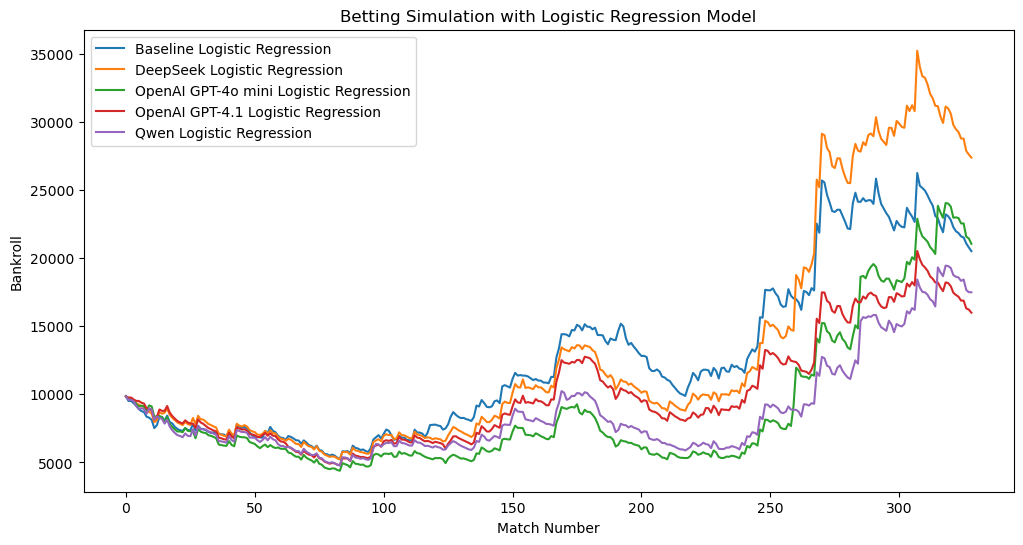
\includegraphics[width=0.48\textwidth]{images/lr_f1.png}
}
\hfill
\subfloat[SVC\label{fig:svc_bankroll_f1}]{%
    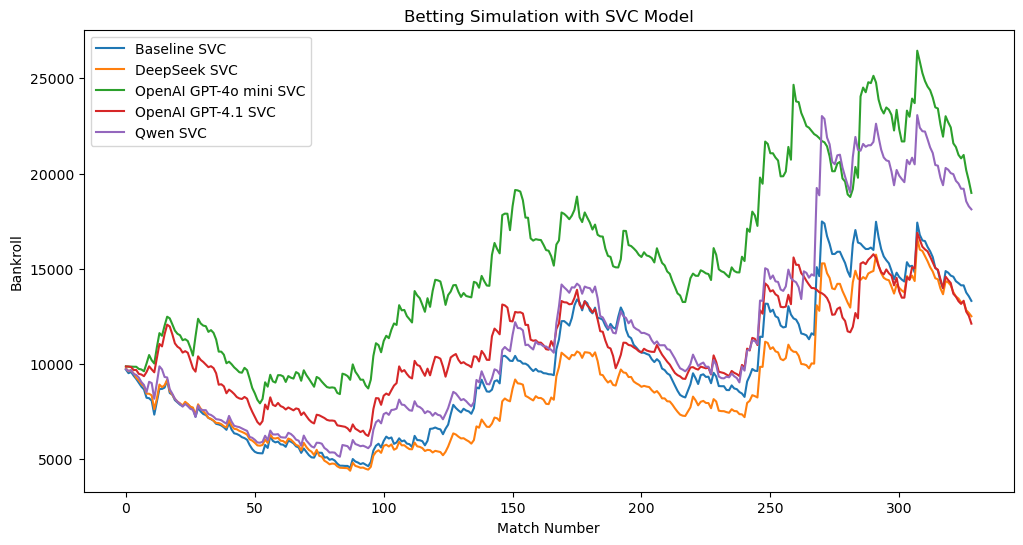
\includegraphics[width=0.48\textwidth]{images/svc_f1.png}
}

\vspace{0.1cm}

\subfloat[Random Forest\label{fig:random_forest_bankroll_f1}]{%
    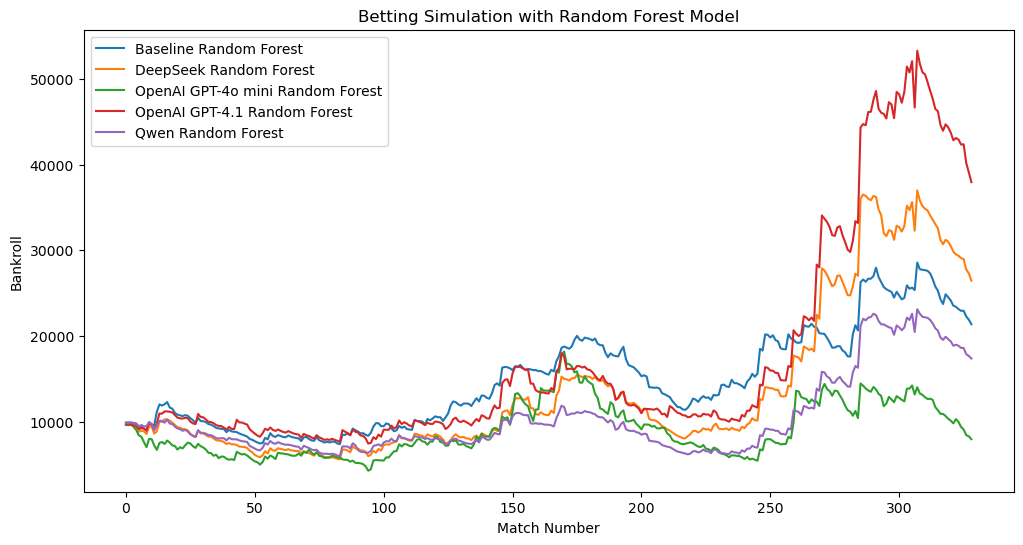
\includegraphics[width=0.48\textwidth]{images/rf_f1.png}
}
\hfill
\subfloat[XGBoost\label{fig:xgboost_bankroll_f1}]{%
    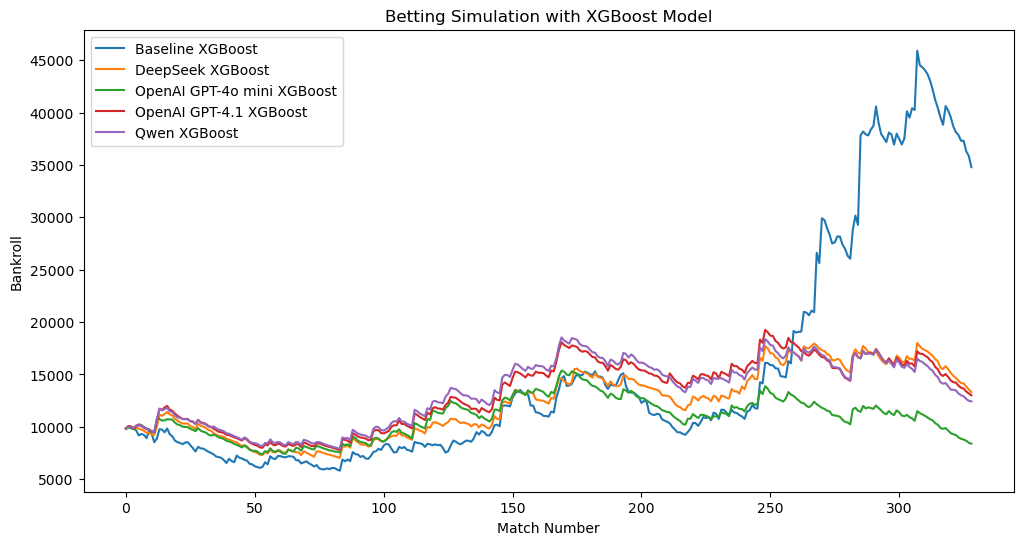
\includegraphics[width=0.48\textwidth]{images/xgboost_f1.png}
}

\caption{Betting simulation bankroll evolution across matches for the 2023-24 EPL season comparing F1-tuned baseline models with their LLM-infused variations across four different machine learning architectures. The results demonstrate that F1-tuned configurations consistently produce more stable growth trajectories and higher final returns.}
\label{fig:betting_evolution}
\end{figure*}

\section{Summary and Implications}
\label{sec:deployment_summary}

This chapter addressed RQ3 by examining deployment configurations, reasoning enhancement techniques, and application strategies that maximize LLM effectiveness across diverse enterprise use cases. The findings connect to and extend the optimization principles established in Chapters~\ref{ch:rag} and \ref{ch:agentic}, demonstrating their applicability across edge deployment, reasoning enhancement, and cross-domain applications.

\subsection{Edge Deployment Guidelines}

\begin{enumerate}[leftmargin=*]
    \item \textbf{Optimal model sizing:} Medium-sized models (7B--32B) achieve the best balance between performance and efficiency for edge deployment. qwen2.5:32b attains 96.75\% ($\pm$0.11\%) F1 with practical inference speeds, while smaller models like qwen2.5:3b achieve 90.89\% F1 with significantly lower resource requirements.
    
    \item \textbf{Quantization effectiveness:} Ollama's Q4\_K\_M quantization enables efficient deployment on consumer hardware while preserving or improving performance compared to bitsandbytes implementations (up to 3.37 percentage point F1 improvement observed).
    
    \item \textbf{Platform optimization:} WSL delivers up to 21$\times$ throughput improvements over native Windows for smaller models, enabling efficient deployment on consumer-grade systems without Linux installation.
    
    \item \textbf{Consumer hardware viability:} For reasoning tasks, models up to 14B parameters are feasible on 16GB consumer GPUs. qwen3:8b offers optimal accuracy-efficiency trade-offs (84.8\% F1, 13GB VRAM, 8.35s inference) for privacy-preserving local deployment.
    
    \item \textbf{Energy considerations:} Small models (1.5B--3B) achieve the highest performance-to-power ratios (0.161--0.163 \%/J), ideal for energy-constrained deployments, while large models (70B+) consume 1,283--1,876 Joules per inference.
\end{enumerate}

\subsection{Reasoning Enhancement Insights}

\begin{enumerate}[leftmargin=*]
    \item \textbf{Open-source competitiveness:} Fine-tuned Qwen2.5 and Llama3.1 models match or exceed GPT-4o on complex reasoning tasks. Qwen2.5-72B achieves 80.88\% F1 on TSQA with only 10-shot prompting, surpassing GPT-4o's 80.36\%. This extends the open-source viability findings from Chapter~\ref{ch:rag} to reasoning-intensive tasks.
    
    \item \textbf{Task-complexity-dependent reasoning effectiveness:} Comprehensive evaluation across 504 configurations reveals that reasoning effectiveness is systematically task-dependent. Base/non-thinking models outperform reasoning variants by $4.8 \pm 6.3$ pp on binary classification (IMDB) and $3.6 \pm 2.2$ pp on 5-class sentiment (Amazon), while reasoning models achieve $2.0 \pm 1.0$ pp advantage on 27-class emotion recognition (GoEmotions). This task-complexity hypothesis provides principled guidance: reserve reasoning for complex multi-class problems where accuracy gains justify 2.1×--54× computational overhead.
    
    \item \textbf{Distillation transfer limitations:} Reasoning patterns optimized for mathematical and logical tasks transfer poorly to simpler sentiment classification. Failure rates decrease with task complexity: 100\% (IMDB), 80\% (Amazon), 50\% (GoEmotions), indicating reasoning distillation becomes more beneficial as classification granularity increases.
    
    \item \textbf{Valid Classification Ratio (VCR):} Novel metric for assessing output reliability beyond accuracy, particularly important for structured classification tasks where invalid outputs cause downstream failures. Fine-tuning improves VCR to $>$98.6\% across evaluated models, with some models improving from as low as 1.17\% to 100\% within 0.2 epochs.
    
    \item \textbf{Reasoning Intensity (RI):} Novel metric capturing the trade-off between explanation depth and computational cost. Three operational regimes identified: Minimal (RI $<$ 0.5), Balanced (0.5--0.85), and Intensive ($>$ 0.85), with balanced regime yielding optimal accuracy-efficiency trade-offs.
    
    \item \textbf{Explainability benefits:} DeepSeek-R1's intrinsic reasoning traces provide transparent decision-making processes without external explanation mechanisms, enhancing auditability for enterprise applications.
    
    \item \textbf{Few-shot learning superiority:} Few-shot learning yields improvements over zero-shot in the vast majority of cases, regardless of reasoning mode, positioning it as a more robust and consistent strategy than reasoning activation for enhancing sentiment analysis performance. DeepSeek-R1 demonstrates approximately 8$\times$ improvement in few-shot efficiency over GPT-4o (30 shots vs. 40 shots for comparable performance).
    
    \item \textbf{Pareto-optimal model selection:} Pareto frontier analysis reveals that base models dominate efficiency-performance trade-offs for most sentiment tasks. IMDB frontier is dominated by base models achieving 97--99\% F1 with minimal latency, while GoEmotions includes reasoning models that justify overhead through accuracy gains.
    
    \item \textbf{Temporal robustness challenges:} All evaluated models exhibit 10--17 percentage point F1 degradation on contemporary data, though reasoning intensity remains stable ($\pm$0.02). This suggests models require periodic updating to maintain accuracy on evolving content.
\end{enumerate}

\subsection{Cross-Domain Application Patterns}

\begin{enumerate}[leftmargin=*]
    \item \textbf{Fine-tuning universality:} Parameter-efficient fine-tuning (LoRA/QLoRA) consistently improves performance across translation, reasoning, and sentiment tasks. The technique enables multi-task adaptation through swappable adapters without full model retraining.
    
    \item \textbf{Zero-shot LLM capabilities:} Modern LLMs effectively extract nuanced signals from unstructured text without domain-specific training, enabling rapid deployment across diverse domains. This was demonstrated in both Chinese-English translation (COMET 0.7324 for Qwen2-72B) and sports sentiment extraction.
    
    \item \textbf{Optimization strategy alignment:} Task-specific optimization dramatically improves practical outcomes. F1 tuning for sports betting produces 2--3$\times$ higher returns than accuracy tuning, demonstrating that metric selection must align with downstream objectives.
    
    \item \textbf{Novel evaluation metrics:} This chapter introduces four domain-specific metrics, complementing the RAP metric from Chapter~\ref{ch:rag} and the ASR/ECR@1 metrics from Chapter~\ref{ch:agentic}:
    \begin{itemize}
        \item \textbf{VCR} (Valid Classification Ratio) for output reliability in classification tasks
        \item \textbf{RI} (Reasoning Intensity) for reasoning-explainability trade-offs
        \item \textbf{TCR} (Translation Completeness Ratio) for translation reliability
        \item \textbf{CPS} (Characters per Second) for translation efficiency
    \end{itemize}
\end{enumerate}

These findings provide practitioners with evidence-based guidelines for deploying LLMs across diverse enterprise contexts, balancing performance, efficiency, explainability, and cost considerations. The research demonstrates that open-source models can achieve enterprise-grade performance when properly optimized, enabling privacy-preserving edge deployment while maintaining competitive accuracy with proprietary alternatives.
\chapter{Conclusions and Future Work}
\label{ch:conclusions}

\section{Summary of Contributions}
\label{sec:contributions_summary}

Having previewed the key contributions organized by type in Chapter~\ref{ch:introduction} (Section~\ref{sec:contributions}), we now provide a detailed synthesis organized by research pillar, reflecting on what was achieved across the research portfolio spanning sixteen publications at premier AI/NLP venues.

This dissertation has systematically investigated optimization strategies for deploying Large Language Models in enterprise applications. The research contributions span three interconnected pillars---Retrieval-Augmented Generation optimization, agentic AI for business automation, and enterprise deployment strategies---supported by cross-domain validation across diverse enterprise applications.

\subsection{RAG Optimization Contributions (Chapter~\ref{ch:rag})}

The first pillar addressed RQ1: \textit{How can RAG systems be optimized to improve response quality while addressing critical issues such as content repetition in open-source LLMs?}

\begin{enumerate}[leftmargin=*]
    \item \textbf{Repetition-Aware Performance (RAP) Metric:} We introduced a novel evaluation metric that addresses a critical gap in assessing open-source LLM outputs. RAP quantifies and penalizes repetition through the formula $\text{RAP} = P \times (1-\text{RR})^3$, enabling effective tuning of the repetition penalty parameter (RPP). Comprehensive experiments across twelve models and three datasets demonstrated that RAP enables up to 93.1\% reduction in repetition with minimal performance degradation (typically under 4\%). The cubic penalty function was validated through ablation studies as optimal across diverse tasks.
    
    \item \textbf{Repetition Detection Algorithm (ReDA):} Complementing the RAP metric, we developed ReDA for systematic identification and quantification of repetitive content in LLM outputs, enabling automated quality assessment in production systems.
    
    \item \textbf{Comparative Evaluation Framework:} Systematic benchmarking on the PCI DSS compliance domain established that smaller, efficient models like Orca-2-13b can achieve competitive---and sometimes superior---performance to proprietary alternatives in RAG applications. Orca-2-13b achieved 99.3\% overall RAGAS score with perfect faithfulness, challenging assumptions that larger models are necessary for high-quality enterprise deployments.
    
    \item \textbf{Evaluation-Guided Hyperparameter Search:} We formalized an optimization procedure using RAP as the target metric, enabling systematic identification of configurations that balance factual accuracy, relevance, and output conciseness.
\end{enumerate}

\subsection{Agentic AI Contributions (Chapter~\ref{ch:agentic})}

The second pillar addressed RQ2: \textit{How can multi-agent LLM architectures be designed to reliably automate complex enterprise workflows while providing measurable reliability guarantees?}

\begin{enumerate}[leftmargin=*]
    \item \textbf{Multi-Agent Invoice Reconciliation System:} We designed and validated a three-agent architecture (Data Engineering, Email, Reconciliation) achieving 99.90\% success rate with the Qwen2.5-32B model---outperforming all proprietary cloud APIs while consuming only 523 Joules per task on consumer hardware (RTX 4090).
    
    \item \textbf{12-Category Error Taxonomy:} We developed a comprehensive diagnostic framework for tool invocation reliability, distinguishing tool initialization, parameter handling, execution, and result interpretation errors. This taxonomy enables systematic failure characterization and targeted improvement strategies for multi-agent systems.
    
    \item \textbf{Agentic Success Rate (ASR):} We introduced a fine-grained metric quantifying tool-calling precision throughout multi-step workflows. ASR decomposes tasks into atomic steps, revealing that smaller models fail primarily at tool orchestration rather than downstream processing---qwen3:32b achieves 98\% ASR matching GPT-4.1 quality.
    
    \item \textbf{Evaluation Completion Rate (ECR@1):} We introduced an operational reliability metric measuring first-attempt evaluation success rates. ECR@1 reveals reliability variations from 85.4\% to 100\% across models, with direct cost implications via retry overhead invisible to accuracy-only evaluation.
    
    \item \textbf{LLM-as-a-Judge (LAJ) Framework:} We developed a production-ready, rubric-driven framework for evaluating Gherkin acceptance tests with structured JSON outputs, revealing 175$\times$ cost variation (\$0.45--\$78.96 per 1K evaluations) and demonstrating that GPT-4o Mini achieves best-in-class accuracy at 78$\times$ cost reduction versus premium models.
    
    \item \textbf{Hierarchical Multi-Agent System for Payments (HMASP):} We designed the first LLM-based multi-agent system for end-to-end agentic payment workflows, featuring a four-level hierarchy with architectural patterns including shared state variables, decoupled message states, and structured handoff protocols, achieving 97.0\% task success rate.
    
    \item \textbf{EdgeAgent Annotation Pipeline:} We developed a semi-automatic interactive annotation system demonstrating that edge-deployed LLMs can achieve annotation quality matching cloud-based proprietary alternatives while preserving data privacy.
\end{enumerate}

\subsection{Enterprise Deployment and Application Contributions (Chapter~\ref{ch:strategies})}

The third pillar addressed RQ3: \textit{What strategies enable effective LLM deployment across diverse enterprise applications, hardware configurations, and domain requirements?}

\begin{enumerate}[leftmargin=*]
    \item \textbf{Comprehensive Edge Deployment Benchmarking:} Systematic evaluation across six hardware platforms (from NVIDIA H100 to consumer laptops and edge devices) established that medium-sized models (7B--32B) achieve optimal performance-efficiency trade-offs. WSL provides up to 21$\times$ speedup over native Windows for smaller models, while Ollama's Q4\_K\_M quantization enables efficient deployment with up to 3.37 percentage point F1 improvement over bitsandbytes implementations.
    
    \item \textbf{Reasoning Intensity (RI) Metric:} We introduced a metric quantifying the proportion of computational effort devoted to reasoning, computed as $\text{RI} = \frac{\text{MRT}}{\text{MRT} + \text{MOT}}$. Three operational regimes were identified: Minimal (RI $<$ 0.5), Balanced (0.5--0.85), and Intensive ($>$ 0.85), with balanced regime yielding optimal accuracy-efficiency trade-offs.
    
    \item \textbf{Valid Classification Ratio (VCR):} We introduced a reliability metric measuring the proportion of valid classifications among total outputs. Fine-tuning dramatically improves VCR from as low as 1.17\% to 100\% within 0.2 epochs, providing practitioners with a concrete measure of deployment readiness for structured classification tasks.
    
    \item \textbf{Task-Complexity-Dependent Reasoning Effectiveness:} Through comprehensive evaluation of 504 configurations across seven model families (DeepSeek-R1, Qwen3, Granite, Magistral, and their base variants), we established that reasoning effectiveness is systematically task-dependent. Base/non-thinking models outperform reasoning variants by $4.8 \pm 6.3$ percentage points on binary classification (100\% failure rate for reasoning) and $3.6 \pm 2.2$ pp on 5-class sentiment (80\% failure rate), while reasoning models achieve $2.0 \pm 1.0$ pp advantage on 27-class emotion recognition (only 14\% failure rate for thinking modes). This task-complexity hypothesis provides principled guidance for model selection.
    
    \item \textbf{Pareto Frontier Analysis:} We conducted the first Pareto frontier analysis of performance versus computational cost for reasoning models in sentiment analysis, demonstrating that base models dominate efficiency-performance trade-offs for most sentiment tasks, with reasoning justified only for complex emotion recognition where 2--4 pp improvements justify 2.1$\times$--54$\times$ computational overhead.
    
    \item \textbf{Translation Completeness Ratio (TCR) and Characters per Second (CPS):} We introduced domain-specific metrics for machine translation reliability and efficiency, addressing the observation that LLMs sometimes produce outputs with untranslated segments.
    
    \item \textbf{Cross-Domain Validation:} Applications across financial prediction, sentiment analysis, machine translation, logical reasoning, and sports predictive analytics validated the generalizability of optimization techniques. F1-tuned models for sports betting achieved 279.48\% returns (Random Forest + GPT-4.1), demonstrating that metric selection must align with downstream objectives.
\end{enumerate}

\subsection{Unifying the Evaluation Metrics for Practice}
\label{sec:metric-synthesis}
This dissertation introduces multiple complementary metrics because enterprise readiness is multi-dimensional: a model can be accurate yet operationally unreliable, cost-prohibitive, or unsuitable under latency and privacy constraints. To reduce practitioner burden, we group the metrics into three layers and recommend a minimal decision workflow:

\begin{itemize}
    \item \textbf{Task quality metrics} (e.g., F1, COMET) quantify whether the system produces correct outputs for the target task.
    \item \textbf{Reliability metrics} (e.g., RAP, VCR, ECR@1, ASR, TCR) quantify whether outputs are usable, complete, and robust under operational conditions (including tool use and constrained formats).
    \item \textbf{Efficiency metrics} (e.g., energy per task, throughput such as CPS) quantify whether the system meets latency, cost, and resource constraints.
\end{itemize}

In practice, we recommend first screening candidate systems by \emph{reliability} (to eliminate configurations that frequently fail, repeat, or violate output constraints), then optimizing \emph{quality} subject to the reliability floor, and finally selecting a configuration that satisfies \emph{efficiency} requirements for the intended deployment tier (cloud, on-prem, or edge).

\section{Key Findings}
\label{sec:key_findings}

Several cross-cutting themes emerge from this research:

\subsection{Finding 1: Open-Source Viability}

\textbf{Open-source LLMs, when properly optimized, achieve performance competitive with---or exceeding---proprietary alternatives across diverse enterprise tasks.}

This finding has significant implications for enterprise AI adoption:
\begin{itemize}[leftmargin=*]
    \item Orca-2-13b achieves 99.3\% RAGAS score in RAG applications (Chapter~\ref{ch:rag}), matching GPT-4
    \item Qwen2.5-72B surpasses GPT-4o on logical reasoning (80.88\% vs. 80.36\% F1) with only 10-shot prompting (Chapter~\ref{ch:strategies})
    \item qwen2.5:32b achieves 99.90\% success rate on invoice reconciliation (Chapter~\ref{ch:agentic}), outperforming all proprietary cloud APIs
    \item qwen3:32b matches GPT-4.1 quality (98\% ASR, 83\% F1) on annotation tasks while enabling edge deployment (Chapter~\ref{ch:agentic})
\end{itemize}

Organizations can leverage open-source models to reduce costs, maintain data privacy through edge deployment, and avoid vendor lock-in while achieving comparable or superior performance.

\subsection{Finding 2: Architecture Over Scale}

\textbf{Larger models do not always outperform smaller counterparts; architectural design and optimization strategies often matter more than parameter count.}

Counter-intuitive findings across multiple studies demonstrate this principle:
\begin{itemize}[leftmargin=*]
    \item DeepSeek-R1:32b (81.7\% F1) substantially outperforms DeepSeek-R1:70b (74.2\% F1) on sentiment analysis (Chapter~\ref{ch:strategies})
    \item 32B Qwen2.5-based distillation outperforms 70B Llama-based variant by 6.69 percentage points (Chapter~\ref{ch:strategies})
    \item qwen3:8b achieves highest performance (84.8\% F1) in its family, surpassing 14B, 30B, and 32B variants (Chapter~\ref{ch:strategies})
    \item Medium-sized models (7B--32B) provide optimal accuracy-efficiency trade-offs for edge deployment (Chapter~\ref{ch:strategies})
    \item Orca-2-13b matches or exceeds GPT-4 performance in RAG applications despite being significantly smaller (Chapter~\ref{ch:rag})
\end{itemize}

Strategic model selection based on task requirements and deployment constraints is essential, as the largest models may not justify additional resource costs.

\subsection{Finding 3: Task Complexity Determines Reasoning Effectiveness}

\textbf{Reasoning capabilities improve performance only for sufficiently complex tasks; simpler tasks often suffer degradation when reasoning is applied.}

Our comprehensive evaluation across 504 configurations reveals systematic task-complexity patterns:
\begin{itemize}[leftmargin=*]
    \item Binary classification (IMDB): 100\% failure rate for reasoning models, $-4.8 \pm 6.3$ pp average degradation
    \item 5-class sentiment (Amazon): 80\% failure rate, $-3.6 \pm 2.2$ pp average degradation
    \item 27-class emotion (GoEmotions): Only 14\% failure rate for thinking modes, $+2.0 \pm 1.0$ pp average improvement
\end{itemize}

This task-complexity hypothesis provides principled deployment guidance: reserve reasoning for complex multi-class problems where accuracy gains justify 2.1$\times$--54$\times$ computational overhead, and leverage base models for simpler classification tasks.

\subsection{Finding 4: Few-Shot Learning Superiority}

\textbf{Few-shot learning yields more robust and consistent improvements than reasoning activation across all task complexities.}

Regardless of whether models are reasoning/thinking-based or base/non-thinking:
\begin{itemize}[leftmargin=*]
    \item Few-shot learning improves over zero-shot in the vast majority of configurations
    \item DeepSeek-R1 achieves 99.31\% accuracy on binary sentiment with just 5 shots, an 8$\times$ improvement in few-shot efficiency over GPT-4o
    \item Performance gains vary by model architecture and task complexity, but the direction is consistently positive
    \item Few-shot prompting enables rapid adaptation without fine-tuning overhead
\end{itemize}

Few-shot prompting provides a more reliable enhancement strategy than reasoning mode activation for sentiment analysis and related classification tasks.

\subsection{Finding 5: Novel Metrics Address Evaluation Gaps}

\textbf{Traditional accuracy metrics are insufficient for enterprise deployment; operational reliability, output quality, and efficiency require dedicated measurement frameworks.}

This dissertation introduces seven complementary metrics addressing distinct evaluation dimensions:

\begin{table}[htbp]
\centering
\caption{Summary of Novel Evaluation Metrics Introduced}
\label{tab:metrics_summary}
\begin{tabular}{@{}llc@{}}
\toprule
\textbf{Metric} & \textbf{Purpose} & \textbf{Chapter} \\
\midrule
RAP & Repetition-aware model evaluation & \ref{ch:rag} \\
VCR & Valid structured output proportion & \ref{ch:strategies} \\
ECR@1 & First-attempt operational reliability & \ref{ch:agentic} \\
ASR & Tool-calling precision in workflows & \ref{ch:agentic} \\
RI & Reasoning-explainability trade-offs & \ref{ch:strategies} \\
TCR & Translation reliability & \ref{ch:strategies} \\
CPS & Translation efficiency & \ref{ch:strategies} \\
\bottomrule
\end{tabular}
\end{table}

These metrics capture operational dimensions essential for enterprise deployment: output quality (RAP), classification reliability (VCR), agentic workflow success (ASR, ECR@1), reasoning efficiency (RI), and translation completeness (TCR, CPS).

\subsection{Finding 6: Modular Multi-Agent Architectures Enable Reliable Automation}

\textbf{Well-designed agent systems with clear specialization, sequential coordination, and appropriate human oversight achieve high reliability even with complex multi-step processes.}

Key architectural principles validated across six multi-agent systems:
\begin{itemize}[leftmargin=*]
    \item Modular agent specialization with clearly defined responsibilities
    \item Hierarchical coordination enabling modular task execution
    \item Information determinism: storing critical data in state variables, not LLM outputs
    \item Structured handoff protocols for inter-agent communication
    \item Human oversight mechanisms for high-impact decisions
\end{itemize}

The 12-category error taxonomy and ASR metric enable systematic diagnosis and improvement of multi-agent system reliability.

\section{Practical Implications}
\label{sec:practical_implications}

For enterprise practitioners, this research provides actionable guidance across the LLM deployment lifecycle:

\subsection{Model Selection}

\begin{enumerate}[leftmargin=*]
    \item Consider mid-tier open-source models (7B--32B) for cost-effective deployments with production-ready reliability
    \item Evaluate task-specific performance rather than relying on general benchmarks
    \item Match reasoning capabilities to task complexity: use base models for simple classification, reserve reasoning for complex multi-class problems
    \item Use proprietary APIs as comparison baselines rather than default choices
    \item For agentic workflows: large models ($\geq$32B) provide production-ready reliability (ASR $>$93\%); small models ($<$4B) are unsuitable for multi-step pipelines
\end{enumerate}

\subsection{Optimization Strategy}

\begin{enumerate}[leftmargin=*]
    \item Invest in systematic hyperparameter tuning using metrics like RAP for RAG systems
    \item Apply targeted fine-tuning for complex reasoning tasks---it consistently outperforms few-shot prompting for deployment reliability (VCR improvements from 1.17\% to 100\%)
    \item Employ chat templates rather than generic prompts for RAG applications to reduce repetition
    \item Align optimization metrics with downstream objectives (e.g., F1 tuning for betting produces 2--3$\times$ higher returns than accuracy tuning)
    \item Leverage few-shot learning as a robust baseline enhancement across all task complexities
\end{enumerate}

\subsection{Evaluation Framework}

\begin{enumerate}[leftmargin=*]
    \item Incorporate RAP alongside traditional accuracy measures for RAG systems
    \item Use VCR to assess output reliability for structured classification tasks
    \item Measure ECR@1 for agentic systems to capture operational reliability and retry costs
    \item Adopt ASR or similar stepwise metrics to diagnose failure modes beyond binary success/failure
    \item Consider Pareto frontier analysis for cost-performance trade-off decisions
    \item Use LLM-as-Judge approaches for scalable evaluation with appropriate cost-reliability trade-offs (175$\times$ cost variation observed)
\end{enumerate}

\subsection{Architecture Design}

\begin{enumerate}[leftmargin=*]
    \item Adopt modular multi-agent designs with clearly defined agent responsibilities for complex workflows
    \item Implement hierarchical coordination for payment and financial processing systems
    \item Store critical information in deterministic state variables, not LLM outputs, to prevent hallucination of sensitive data
    \item Define structured handoff protocols for inter-agent communication
    \item Incorporate human oversight mechanisms for high-impact decisions
    \item Budget 5--15\% overhead for reliability failures and implement appropriate retry logic
\end{enumerate}

\subsection{Infrastructure Planning}

\begin{enumerate}[leftmargin=*]
    \item Consumer-grade GPUs (RTX 4090, 24GB) support models up to 14B parameters for reasoning tasks
    \item Professional workstations (48GB+ VRAM) enable 32B--70B model deployment
    \item Consider Ollama's Q4\_K\_M quantization to extend hardware capabilities with minimal performance loss
    \item WSL provides up to 21$\times$ throughput improvements over native Windows for smaller models
    \item Apple Silicon (M3/M4 Max) provides competitive performance for edge scenarios
    \item Small models (1.5B--3B) achieve highest performance-to-power ratios (0.161--0.163 \%/J) for energy-constrained deployments
\end{enumerate}

% =========================
% Drop-in replacement text (ready to paste)
% Suggested placement: Chapter 6 (Limitations) + a short synthesis in Conclusions
% =========================

\subsection{Limitations and Threats to Validity}
\label{sec:limitations}

While the proposed metrics, architectures, and deployment guidelines are empirically validated across multiple tasks, models, and hardware configurations, several limitations should be noted.

\subsubsection{Scope and Generalizability}
\label{sec:limitations-scope}
The experiments cover a broad range of enterprise-relevant tasks (e.g., retrieval-augmented generation, agentic workflows, sentiment classification, machine translation, and domain-specific analytics). However, the conclusions may not fully generalize to domains with substantially different constraints or data characteristics (e.g., highly specialized biomedical text, low-resource languages, or long-context legal discovery pipelines). In particular, domain shift can affect both retrieval quality (for RAG) and downstream decision reliability (for agentic systems), and thus deployment recommendations should be revalidated when the target domain differs materially from the evaluation settings.

\subsubsection{Dataset and Benchmark Bias}
\label{sec:limitations-benchmark-bias}
Several evaluations rely on established public benchmarks that are primarily English-centric and may not represent the distribution of enterprise documents encountered in production (e.g., internal memos, proprietary templates, multilingual mixed-format documents). This creates potential bias in reported performance and reliability. Future work should extend evaluation to multilingual, format-diverse, and organization-specific corpora to better quantify robustness under real enterprise data distributions.

\subsubsection{Model and Version Volatility}
\label{sec:limitations-volatility}
The LLM landscape evolves rapidly, with frequent model releases, parameter updates, and changes in inference stacks. As a result, absolute performance numbers may drift over time, and direct replication can be challenging when (i) model checkpoints are updated, (ii) system prompts or safety layers change, or (iii) inference frameworks alter kernel-level optimizations. To mitigate this, we report configurations and settings where possible and emphasize \emph{comparative} and \emph{principled} findings (e.g., task-dependent reasoning effectiveness, reliability failure modes, and trade-offs between accuracy, cost, and energy) that are expected to remain more stable than any single point estimate.

\subsubsection{Reproducibility Constraints for Proprietary Models}
\label{sec:limitations-proprietary}
Some baselines involve proprietary models accessed via hosted APIs. These systems may change without notice, and full transparency into training data, decoding strategies, and infrastructure-level optimizations is unavailable. Consequently, comparisons between open-weight and proprietary models may be affected by unobserved factors beyond the researcher's control. Where feasible, we triangulate findings using multiple model families and focus on reproducible open-weight configurations to strengthen external validity.

\subsubsection{Operational Assumptions in Agentic Systems}
\label{sec:limitations-agentic}
Agentic evaluations necessarily assume specific tool interfaces, orchestration frameworks, and workflow definitions. Real deployments can introduce additional failure modes---for example, authentication issues, rate limits, upstream service outages, tool schema changes, or human-in-the-loop delays. Although the proposed error taxonomy and reliability metrics capture core failure patterns, deployment teams should treat them as a foundation and extend them to include infrastructure- and organization-specific operational risks.


\section{Future Research Directions}
\label{sec:future_directions}

Based on the findings and limitations of this research, several promising directions for future work emerge:

\subsection{Advanced RAG Architectures}

Future research should explore RAG systems that dynamically adjust retrieval strategies:
\begin{itemize}[leftmargin=*]
    \item Query-dependent chunk selection and filtering
    \item Iterative retrieval with progressive refinement
    \item Multi-stage retrieval combining sparse and dense methods
    \item Self-evaluating RAG with automatic quality assessment using RAP-like metrics
    \item Integration of repetition penalty optimization into the retrieval pipeline
\end{itemize}

\subsection{Adaptive Reasoning Architectures}

Our task-complexity findings motivate research into systems that dynamically adjust reasoning intensity:
\begin{itemize}[leftmargin=*]
    \item Hybrid architectures that trigger costly reasoning only when ambiguity warrants it
    \item Query-complexity detection to route requests to appropriate reasoning modes
    \item Adaptive thinking budgets that balance accuracy gains against computational overhead
    \item Task-specific distillation objectives tailored to affective reasoning rather than generic logical skills
    \item Empirical investigation of the task-complexity threshold where reasoning transitions from harmful to beneficial, potentially enabling automated routing decisions
\end{itemize}

\subsection{Enhanced Multi-Agent Coordination}

Building on our multi-agent foundations, future work should investigate:
\begin{itemize}[leftmargin=*]
    \item Dynamic agent allocation based on task complexity and ASR predictions
    \item Learning-based coordination protocols optimized via the 12-category error taxonomy
    \item Fault-tolerant architectures with graceful degradation informed by ECR@1 patterns
    \item Hybrid human-agent workflows with adaptive automation levels
    \item Cross-domain transfer of agentic patterns from payments to other financial processes
\end{itemize}

\subsection{Multimodal Enterprise Applications}

The intersection of agentic AI with emerging modalities presents opportunities:
\begin{itemize}[leftmargin=*]
    \item Vision-language agents for document understanding extending invoice reconciliation
    \item Speech-enabled enterprise assistants with reasoning capabilities
    \item Video analysis for quality control and monitoring
    \item Multimodal sentiment analysis combining text and visual signals
\end{itemize}

\subsection{Continual Learning and Adaptation}

Our temporal robustness findings (10--17 pp degradation on contemporary data) motivate research into models that adapt over time:
\begin{itemize}[leftmargin=*]
    \item Techniques for updating models with new domain knowledge
    \item Methods for detecting and handling distribution shift
    \item Efficient fine-tuning for rapid customization
    \item Knowledge retention strategies to prevent catastrophic forgetting
    \item Periodic RAP recalibration as language patterns evolve
\end{itemize}

\subsection{Sustainable AI Deployment}

Our energy efficiency findings (performance-to-power ratios varying from 0.05 to 0.163 \%/J) motivate research into:
\begin{itemize}[leftmargin=*]
    \item Energy-efficient inference techniques optimized for edge deployment
    \item Carbon-aware model selection and scheduling
    \item Lifecycle assessment of AI system deployment
    \item Trade-offs between accuracy, reasoning intensity, and environmental impact
\end{itemize}

\section{Concluding Remarks}
\label{sec:concluding_remarks}

The rapid advancement of Large Language Models presents both opportunities and challenges for enterprise adoption. This dissertation has demonstrated that systematic optimization---spanning model selection, hyperparameter tuning, prompting strategies, fine-tuning, architectural design, and evaluation methodology---enables effective deployment of LLMs for diverse business applications.

The research establishes that open-source models, when properly optimized, can achieve performance competitive with proprietary alternatives while offering advantages in customization, privacy, and cost. Across sixteen publications at premier venues, we demonstrated this principle in RAG systems (Orca-2-13b matching GPT-4), logical reasoning (Qwen2.5-72B surpassing GPT-4o), multi-agent automation (qwen2.5:32b outperforming cloud APIs), and annotation pipelines (qwen3:32b matching GPT-4.1).

A central contribution is the recognition that reasoning effectiveness is task-dependent. The comprehensive evaluation across 504 configurations challenges the prevailing narrative that enhanced reasoning universally improves LLM performance. For simple binary classification, reasoning introduces noise rather than clarity; for complex 27-class emotion recognition, reasoning provides measurable benefits. This task-complexity hypothesis offers principled guidance for practitioners navigating the expanding landscape of reasoning-capable models.

A distinguishing methodological contribution is the development of seven novel evaluation metrics that capture operational dimensions invisible to traditional accuracy-focused assessment. These metrics---RAP, VCR, ECR@1, ASR, RI, TCR, and CPS---provide practitioners with concrete, measurable targets for deployment readiness across the three research pillars. Table~\ref{tab:metrics_summary} summarizes these contributions, demonstrating how the dissertation addresses evaluation gaps across RAG systems, agentic workflows, and enterprise deployment scenarios.

Multi-agent architectures represent a promising paradigm for automating complex workflows that traditionally require human coordination. Our invoice reconciliation system demonstrates that edge-deployed open-source models can outperform cloud APIs while maintaining privacy and reducing operational costs. The 12-category error taxonomy and ASR metric provide systematic tools for diagnosing and improving multi-agent reliability.

Perhaps most importantly, this research emphasizes that thoughtful engineering of the entire deployment pipeline---not merely model selection---determines success in enterprise AI applications. The contributions, guidelines, and insights presented here provide a foundation for responsible and effective integration of generative AI into enterprise operations.

As LLM capabilities continue to advance, the optimization principles established in this dissertation will require ongoing refinement. However, the fundamental insight remains: bridging the gap between AI potential and practical deployment requires systematic attention to evaluation, optimization, and architecture across the entire system lifecycle. The demonstrated success of open-source models on consumer hardware significantly reduces barriers to enterprise AI adoption, enabling organizations of all sizes to deploy sophisticated AI systems while maintaining control over their data, costs, and operational requirements.

% ============ BIBLIOGRAPHY ============
\singlespacing\small
\bibliography{references}

% ============ APPENDICES ============
\appendix
\chapter{Supplementary Materials}
\label{app:supplementary}

This appendix provides detailed specifications, configurations, and reference materials supporting the experimental work presented in Chapters~\ref{ch:rag}--\ref{ch:strategies}. Section~\ref{app:model_specs} catalogs all evaluated models; Section~\ref{app:hardware} details hardware platforms; Section~\ref{app:exp_configs} presents experimental configurations; Section~\ref{app:invoice_errors} illustrates multi-agent error patterns; Section~\ref{app:prompts} documents prompt templates; and Section~\ref{app:metrics} consolidates the seven novel evaluation metrics introduced throughout this dissertation.

\section{Complete Model Specifications}
\label{app:model_specs}

Table~\ref{tab:full_model_specs} provides detailed specifications for all models evaluated in this dissertation, organized by model family. Models are grouped into proprietary alternatives (used as comparison baselines), reasoning-specialized architectures (central to Chapter~\ref{ch:strategies}), and general-purpose open-source models (evaluated across all three research pillars).

\begin{longtable}{@{}p{3.5cm}p{1.8cm}p{2cm}p{2.2cm}p{3cm}@{}}
\caption{Complete Model Specifications} \label{tab:full_model_specs} \\
\toprule
\textbf{Model} & \textbf{Parameters} & \textbf{Context} & \textbf{Architecture} & \textbf{Notes} \\
\midrule
\endfirsthead
\multicolumn{5}{c}{{\tablename\ \thetable{} -- continued from previous page}} \\
\toprule
\textbf{Model} & \textbf{Parameters} & \textbf{Context} & \textbf{Architecture} & \textbf{Notes} \\
\midrule
\endhead
\midrule
\multicolumn{5}{r}{{Continued on next page}} \\
\endfoot
\bottomrule
\endlastfoot
\multicolumn{5}{c}{\textit{Proprietary Models (Comparison Baselines)}} \\
\midrule
GPT-4 & Undisclosed & 128K & MoE (speculated) & OpenAI; RAG baseline \\
GPT-4o & Undisclosed & 128K & Multimodal & OpenAI; sentiment/reasoning \\
GPT-4o-mini & Undisclosed & 128K & Multimodal & OpenAI; cost-optimized \\
GPT-4.1 & Undisclosed & 1M & Multimodal & OpenAI, Apr 2025; agentic \\
GPT-4.1-nano & Undisclosed & 1M & Multimodal & OpenAI; edge annotation \\
GPT-4.1-mini & Undisclosed & 1M & Multimodal & OpenAI; LAJ framework \\
Claude Sonnet 4 & Undisclosed & 200K & Decoder-only & Anthropic; agentic eval \\
\midrule
\multicolumn{5}{c}{\textit{DeepSeek Family}} \\
\midrule
DeepSeek-V3 & 671B & 128K & MoE & Base model for DSR1 \\
DeepSeek-R1 (Full) & 671B & 128K & MoE & RL-trained reasoning \\
DeepSeek-R1:8B & 8B & 64K & Decoder-only & Distilled from Llama3.1-8B \\
DeepSeek-R1:14B & 14B & 64K & Decoder-only & Distilled from Qwen2.5-14B \\
DeepSeek-R1:32B & 32B & 64K & Decoder-only & Distilled from Qwen2.5-32B \\
DeepSeek-R1:70B & 70B & 64K & Decoder-only & Distilled from Llama3.3-70B \\
\midrule
\multicolumn{5}{c}{\textit{Qwen Family}} \\
\midrule
Qwen2-7B & 7B & 128K & Decoder-only & Translation experiments \\
Qwen2-72B & 72B & 128K & Decoder-only & Translation; fine-tuning \\
Qwen2.5-0.5B & 0.5B & 128K & Decoder-only & Edge deployment \\
Qwen2.5-1.5B & 1.5B & 128K & Decoder-only & Edge deployment \\
Qwen2.5-3B & 3B & 128K & Decoder-only & Edge deployment \\
Qwen2.5-7B & 7B & 128K & Decoder-only & 18T tokens; RAG/edge \\
Qwen2.5-14B & 14B & 128K & Decoder-only & Base for DSR1-14B \\
Qwen2.5-32B & 32B & 128K & Decoder-only & Base for DSR1-32B; agentic \\
Qwen2.5-72B & 72B & 128K & Decoder-only & 18T tokens; reasoning \\
Qwen2.5-Plus & API & 128K & Decoder-only & Soccer betting sentiment \\
Qwen3-0.6B & 0.6B & 32K & Decoder-only & T/N modes \\
Qwen3-1.7B & 1.7B & 32K & Decoder-only & T/N modes \\
Qwen3-4B & 4B & 32K & Decoder-only & T/N modes \\
Qwen3-8B & 8B & 32K & Decoder-only & T/N modes; best Qwen3 \\
Qwen3-14B & 14B & 32K & Decoder-only & T/N modes \\
Qwen3-30B & 30B & 32K & Decoder-only & T/N modes \\
Qwen3-32B & 32B & 32K & Decoder-only & T/N modes; annotation \\
\midrule
\multicolumn{5}{c}{\textit{Llama Family}} \\
\midrule
Llama-2-7B & 7B & 4K & Decoder-only & 2T tokens \\
Llama-2-13B & 13B & 4K & Decoder-only & 2T tokens \\
Llama-2-70B & 70B & 4K & Decoder-only & 2T tokens \\
Llama-3-8B & 8B & 8K & Decoder-only & 15T tokens \\
Llama-3-70B & 70B & 8K & Decoder-only & 15T tokens \\
Llama-3.1-8B & 8B & 128K & Decoder-only & Base for DSR1-8B; edge \\
Llama-3.1-70B & 70B & 128K & Decoder-only & 15T+ tokens; fine-tuning \\
Llama-3.2-1B & 1B & 128K & Decoder-only & Edge-optimized \\
Llama-3.2-3B & 3B & 128K & Decoder-only & Edge-optimized \\
Llama-3.2-vision:11B & 11B & 128K & Multimodal & Vision-language; edge \\
Llama-3.2-vision:90B & 90B & 128K & Multimodal & Vision-language \\
Llama-3.3-70B & 70B & 128K & Decoder-only & Base for DSR1-70B \\
\midrule
\multicolumn{5}{c}{\textit{Reasoning-Specialized Models}} \\
\midrule
Granite3.3-2B & 2B & 128K & Decoder-only & IBM; T/N modes \\
Granite3.3-8B & 8B & 128K & Decoder-only & IBM; T/N modes \\
Magistral-24B & 24B & 128K & Decoder-only & Mistral; RL reasoning \\
GPT-OSS:20B (low) & 20B & 32K & Decoder-only & Minimal reasoning (RI$<$0.5) \\
GPT-OSS:20B (medium) & 20B & 32K & Decoder-only & Balanced reasoning \\
GPT-OSS:20B (high) & 20B & 32K & Decoder-only & Intensive reasoning (RI$>$0.85) \\
GPT-OSS:120B (low) & 120B & 32K & Decoder-only & Minimal reasoning \\
GPT-OSS:120B (medium) & 120B & 32K & Decoder-only & Balanced; best F1 (86.2\%) \\
GPT-OSS:120B (high) & 120B & 32K & Decoder-only & Intensive reasoning \\
\midrule
\multicolumn{5}{c}{\textit{Other Open-Source Models}} \\
\midrule
Orca-2-7B & 7B & 4K & Decoder-only & Synthetic training \\
Orca-2-13B & 13B & 4K & Decoder-only & Synthetic; RAG champion \\
Mistral-7B & 7B & 32K & Decoder-only & Sliding window attn. \\
Phi-3.5-mini & 3.8B & 128K & Decoder-only & Synthetic training \\
Gemma-2B & 2B & 8K & Decoder-only & Google; 2T tokens \\
Gemma-7B & 7B & 8K & Decoder-only & Google; 6T tokens \\
InternLM2.5-7B & 7B & 32K & Decoder-only & Shanghai AI Lab \\
InternLM2.5-7B-1M & 7B & 1M & Decoder-only & Extended context; reasoning \\
InternLM2.5-20B & 20B & 32K & Decoder-only & Shanghai AI Lab \\
Functionary-small & 8B & 32K & Function-calling & Tool-optimized; agentic \\
Functionary-medium & 70B & 32K & Function-calling & Tool-optimized; agentic \\
\end{longtable}

\textbf{Notes:} 
\begin{itemize}[leftmargin=*]
    \item T/N modes = Thinking/Non-thinking modes with runtime-activated reasoning (Section~\ref{subsec:task_complexity})
    \item MoE = Mixture of Experts architecture
    \item RI = Reasoning Intensity metric introduced in Section~\ref{subsec:reasoning_deployment}
    \item Context lengths represent maximum supported; actual usage may vary by deployment configuration
    \item Models marked ``edge'' were evaluated across consumer hardware platforms (Section~\ref{subsec:ollama_edge})
    \item Models marked ``agentic'' were evaluated in multi-agent workflows (Chapter~\ref{ch:agentic})
\end{itemize}

\section{Hardware Specifications}
\label{app:hardware}

Table~\ref{tab:hardware_specs} details the six primary hardware platforms used for evaluation in this dissertation, spanning enterprise GPUs, consumer hardware, and edge devices. These platforms correspond to the edge deployment evaluation in Section~\ref{subsec:ollama_edge}.

\begin{table}[htbp]
\centering
\caption{Hardware Platforms for Model Evaluation}
\label{tab:hardware_specs}
\resizebox{\textwidth}{!}{%
\begin{tabular}{@{}p{3.5cm}p{9cm}@{}}
\toprule
\textbf{Platform} & \textbf{Specifications} \\
\midrule
\multicolumn{2}{c}{\textit{Enterprise GPU}} \\
\midrule
NVIDIA H100 & 96GB HBM3 VRAM, 16,896 CUDA cores, 528 Tensor cores, PCIe 5.0, 3.9 TB/s bandwidth, Ubuntu 24.04.1 LTS, CUDA 12.4, Ollama 0.11.4 \\
\midrule
\multicolumn{2}{c}{\textit{Professional Workstation}} \\
\midrule
NVIDIA RTX A6000 Ada & 48GB GDDR6 ECC VRAM, 18,176 CUDA cores, 568 Tensor cores, AMD Threadripper PRO 5975WX (32 cores), 256GB DDR4-3200 ECC, Ubuntu 22.04 LTS / Windows 11 Pro + WSL2 \\
\midrule
\multicolumn{2}{c}{\textit{Consumer Desktop}} \\
\midrule
NVIDIA RTX 4090 & 24GB GDDR6X VRAM, 16,384 CUDA cores, 512 Tensor cores, Intel Core i9-13900K (24 cores), 64GB DDR5-5600, Ubuntu 22.04 LTS via WSL2, CUDA 12.1, Ollama 0.5.4--0.6.8 \\
\midrule
\multicolumn{2}{c}{\textit{Consumer Laptop}} \\
\midrule
NVIDIA RTX 4090 Laptop & 16GB GDDR6 VRAM, 9,728 CUDA cores, 304 Tensor cores, Intel Core i9-14900HX, 64GB DDR5, Windows 11 Pro / WSL2 Ubuntu 22.04 (\textbf{21$\times$ speedup over native Windows for small models}) \\
\midrule
\multicolumn{2}{c}{\textit{Apple Silicon}} \\
\midrule
M3 Max MacBook Pro & 96GB Unified Memory, 16-core CPU, 40-core GPU, 16-core Neural Engine, macOS Sequoia 15.4, MLX 0.12.0, Ollama 0.5.4 \\
M4 Max MacBook Pro & 48GB Unified Memory, 16-core CPU, 40-core GPU, 16-core Neural Engine, macOS Sequoia 15.1, Ollama 0.5.4 \\
\midrule
\multicolumn{2}{c}{\textit{Edge Device}} \\
\midrule
NVIDIA Jetson AGX Orin & 64GB LPDDR5 Memory, 2,048 CUDA cores, 64 Tensor cores, 12-core Arm Cortex-A78AE CPU, up to 275 TOPS INT8, JetPack 6.0, Ubuntu 20.04 \\
\bottomrule
\end{tabular}
}
\end{table}

\subsection{Platform Selection Rationale}

The hardware platforms were selected to represent the full spectrum of enterprise deployment scenarios addressed in Chapter~\ref{ch:strategies}:

\begin{itemize}[leftmargin=*]
    \item \textbf{H100:} Cloud/data center deployments requiring maximum throughput; primary platform for 504-configuration task complexity evaluation (Section~\ref{subsec:task_complexity})
    \item \textbf{RTX A6000 Ada:} Professional workstations for development and medium-scale inference; energy efficiency evaluation (Figure~\ref{fig:energy_efficiency})
    \item \textbf{RTX 4090 Desktop:} Cost-effective on-premises deployment with strong performance; multi-agent invoice reconciliation (Chapter~\ref{ch:agentic}), achieving 99.90\% success rate with qwen2.5:32b at 523 Joules per task
    \item \textbf{RTX 4090 Laptop:} Mobile professional use cases; 16GB VRAM constraint defines viable reasoning models (qwen3:8b optimal at 84.8\% F1, 13GB VRAM)
    \item \textbf{Apple Silicon:} macOS-native deployment and unified memory advantages; competitive edge performance
    \item \textbf{Jetson AGX Orin:} Edge deployment for privacy-sensitive and latency-critical applications
\end{itemize}

\subsection{Key Hardware Findings Summary}

The following hardware-specific findings from Section~\ref{subsec:ollama_edge} inform deployment decisions:

\begin{enumerate}[leftmargin=*]
    \item \textbf{WSL Performance:} Windows Subsystem for Linux delivers up to 21$\times$ throughput improvement over native Windows for smaller models (qwen2.5:0.5b: 16,933 vs. 816 tokens/s on RTX A6000)
    \item \textbf{VRAM Constraints:} Consumer 16GB GPUs support models up to 14B parameters for reasoning tasks; 24GB enables 32B deployment
    \item \textbf{Cross-Platform Stability:} Larger models exhibit increased consistency (F1 std: 0.07--0.23\%) compared to small models (0.26--0.90\%)
    \item \textbf{Energy Efficiency:} Small models (1.5B--3B) achieve highest performance-to-power ratios (0.161--0.163 \%/J); large models consume 1,283--1,876 Joules per inference
\end{enumerate}

\section{Detailed Experimental Configurations}
\label{app:exp_configs}

\subsection{RAG Experiments Configuration (Chapter~\ref{ch:rag})}

\begin{verbatim}
# Embedding Model Configuration
embedding_model: hkunlp/instructor-large
embedding_dim: 768
max_seq_length: 512

# Retrieval Configuration
vector_store: FAISS
index_type: IVF_FLAT
num_clusters: 100
top_k_retrieval: 10

# Chunking Configuration
chunk_size: 500  # tokens
chunk_overlap: 50  # tokens
separator: "\n\n"

# Generation Configuration
temperature: 0.7
max_new_tokens: 1024
top_p: 0.95
repetition_penalty: 1.0-1.2  # varied in experiments

# RAP Metric Configuration
rap_exponent: 3  # cubic penalty validated via ablation
performance_metric: RAGAS_composite  # or task-specific F1

# Hardware
gpu: NVIDIA RTX 4090 (24GB) / A6000 (48GB)
precision: float16
\end{verbatim}

\subsection{Fine-Tuning Configuration (Chapters~\ref{ch:rag}, \ref{ch:strategies})}

\begin{verbatim}
# LoRA Configuration
lora_r: 64
lora_alpha: 128
lora_dropout: 0.1
target_modules: ["q_proj", "v_proj", "k_proj", "o_proj"]

# Training Configuration
learning_rate: 2e-4
batch_size: 8
gradient_accumulation_steps: 4
num_epochs: 3  # with early stopping at 0.2 epoch granularity
warmup_ratio: 0.1
weight_decay: 0.01
optimizer: AdamW

# QLoRA Specific (for models >= 20B)
quantization_bits: 4
bnb_4bit_compute_dtype: float16
bnb_4bit_quant_type: nf4
bnb_4bit_use_double_quant: True

# Early Stopping (per Section 5.3.1.5)
# Larger models peak earlier: 0.8 epochs (72B) vs 1.0 epochs (7B)
# VCR improves from 1.17% to 100% within 0.2 epochs
\end{verbatim}

\subsection{Multi-Agent System Configuration (Chapter~\ref{ch:agentic})}

\begin{verbatim}
# LangGraph Configuration
graph_type: StateGraph
checkpoint_store: MemorySaver
recursion_limit: 25

# Agent Configuration
max_iterations: 10
tool_timeout: 30  # seconds
retry_attempts: 3

# Database Configuration
db_type: SQLite
connection_mode: in-memory

# Email Agent Configuration
imap_server: imap.gmail.com
smtp_server: smtp.gmail.com
fetch_limit: 50

# Ollama Configuration (Edge Deployment)
ollama_version: 0.6.8
quantization: Q4_K_M
context_length: 8192

# HMASP Four-Level Hierarchy
hierarchy_levels: [orchestrator, domain_supervisors, 
                   specialized_agents, tools]
shared_state_variables: true
decoupled_message_states: true
structured_handoff_protocols: true

# Success Metrics
target_ASR: 0.93  # minimum for production-ready
target_TSR: 0.97  # task success rate
ECR_retry_budget: 0.15  # 15% overhead for reliability failures
\end{verbatim}

\subsection{Task Complexity Experiments Configuration (Section~\ref{subsec:task_complexity})}

The following configuration was used for the 504-configuration evaluation of reasoning effectiveness across sentiment analysis tasks.

\begin{verbatim}
# Model Families Evaluated (7 families)
deepseek_r1: [671B-full, 8B, 14B, 32B, 70B]
deepseek_v3: [671B]  # Base model comparison
llama_bases: [3.1-8B, 3.3-70B]
qwen25_bases: [14B, 32B]
qwen3: [4B, 8B, 14B, 30B, 32B]  # T/N modes
granite33: [2B, 8B]  # T/N modes
magistral: [24B]  # T/N modes

# Datasets (3 complexity levels)
imdb:
  task: binary_sentiment
  classes: [Positive, Negative]
  test_size: 1000
  complexity: simple
  expected_reasoning_benefit: negative  # -4.8 pp avg

amazon_reviews:
  task: 5class_sentiment
  classes: [Strongly Negative, Negative, Neutral, 
            Positive, Strongly Positive]
  test_size: 1838  # human-annotated
  complexity: moderate
  expected_reasoning_benefit: mixed  # -3.6 pp avg

goemotions:
  task: 27class_emotion
  classes: [admiration, amusement, anger, annoyance,
            approval, caring, confusion, curiosity,
            desire, disappointment, disapproval, disgust,
            embarrassment, excitement, fear, gratitude,
            grief, joy, love, nervousness, optimism,
            pride, realization, relief, remorse, 
            sadness, surprise]
  test_size: 1000
  complexity: high
  expected_reasoning_benefit: positive  # +2.0 pp avg
  note: single-label subset only

# Few-Shot Configuration (7 levels)
shot_levels: [0, 5, 10, 20, 30, 40, 50]
sampling_strategy: stratified
random_seed: 42

# Inference Configuration
ollama_version: 0.6.8
quantization: Q4_K_M  # MXFP4 for GPT-OSS
context_length: 8192
temperature: 0.0  # deterministic
max_tokens: 256

# Hardware
primary: NVIDIA H100 (96GB)
validation: NVIDIA RTX 4090 (24GB)
cross_platform: [M3 Max, RTX 4090 Laptop]  # temporal robustness

# Metrics Computed
performance: [F1, Accuracy, Weighted-F1]
efficiency: [mean_latency_per_sample, VRAM_usage, speed_ratio]
reasoning: [MRT, MOT, RI]  # Mean Reasoning/Output Tokens

# Pareto Frontier Analysis
pareto_axes: [F1_score, log_latency]
frontier_identification: non-dominated_sorting
\end{verbatim}

\textbf{Configuration Notes:}
\begin{itemize}[leftmargin=*]
    \item Total configurations: 7 model families $\times$ 3 datasets $\times$ 7 shot levels $\times$ T/N variants = 504
    \item DeepSeek-R1 (full) and DeepSeek-V3 accessed via official API; all others via Ollama
    \item Thinking (T) and Non-thinking (N) modes evaluated separately for Qwen3, Granite3.3, and Magistral
    \item Stratified sampling ensures balanced class representation in few-shot exemplars
    \item Failure rates by dataset: IMDB 100\%, Amazon 80\%, GoEmotions 50\% (reasoning underperforms)
\end{itemize}

\subsection{Reasoning Deployment Experiments Configuration (Section~\ref{subsec:reasoning_deployment})}

\begin{verbatim}
# Model Families (17 variants)
deepseek_r1: [8B, 14B, 32B, 70B]
qwen3: [0.6B, 1.7B, 4B, 8B, 14B, 30B, 32B]
gpt_oss: [20B-low, 20B-medium, 20B-high,
          120B-low, 120B-medium, 120B-high]

# Dataset
amazon_reviews_5class:
  train_split: 70%
  test_split: 30%
  total_samples: 1838

# Temporal Robustness Evaluation
testset2:
  samples: 574
  collection_date: mid-2025
  annotation: manual

# Quantization
deepseek_qwen: Q4_K_M
gpt_oss: MXFP4

# Ollama Configuration
version: 0.11.4
context_length: 8192

# Reasoning Intensity (RI) Regimes
minimal: RI < 0.5      # GPT-OSS low configurations
balanced: 0.5 <= RI <= 0.85  # optimal regime
intensive: RI > 0.85   # DeepSeek-R1 models

# Consumer Hardware Constraint
rtx_4090_laptop_vram: 16GB
viable_models: [qwen3:8b (13GB), qwen3:4b (11GB), 
                qwen3:1.7b (6.8GB)]
optimal_choice: qwen3:8b  # 84.8% F1, 8.35s inference
\end{verbatim}

\subsection{Soccer Betting Experiments Configuration (Section~\ref{subsec:soccer_betting})}

\begin{verbatim}
# Data Sources
match_statistics: API-Football
seasons: 2015-16 to 2023-24 (9 seasons)
betting_odds: Football-Data.co.uk (BetFair 1X2)
commentaries: BBC Sport (Python Selenium scraping)

# Data Partitioning
feature_selection: 2015-19
training: 2015-22
testing: 2022-23
betting_simulation: 2023-24

# LLM Sentiment Analysis
models: [DeepSeek-R1, GPT-4o-mini, GPT-4.1, Qwen2.5-Plus]
prompting: zero-shot
sentiment_scale: 1-5 (Strongly Negative to Strongly Positive)
feature_computation: home_sentiment - away_sentiment

# Machine Learning Models
classifiers: [LogisticRegression, SVC, RandomForest, XGBoost]
tuning_strategies: [accuracy-tuned, F1-tuned]
hyperparameter_search: GridSearchCV
cross_validation: 5-fold

# Betting Simulation
initial_bankroll: $10,000
kelly_fraction: 0.125  # one-eighth Kelly
bet_condition: positive_expected_value

# Key Results Reference
best_return: 279.48%  # Random Forest + GPT-4.1 (F1-tuned)
second_best: 247.97%  # XGBoost Baseline (F1-tuned)
third_best: 174.01%   # Logistic Regression + DeepSeek-R1 (F1-tuned)
\end{verbatim}

\section{Invoice Reconciliation Error Examples}
\label{app:invoice_errors}

The following examples illustrate the three outcome categories tracked by the multi-agent invoice reconciliation system (Chapter~\ref{ch:agentic}). These examples demonstrate the diagnostic value of the structured error taxonomy and ASR metric introduced in Section~\ref{sec:diagnostic_framework}.

\subsection{SUCCESS Example}

\begin{verbatim}
Input: Reconcile invoice INV-2024-001 for customer ABC Corp
       with recent email communications.

Agent Trace:
1. Data Engineering Agent: Retrieved invoice details
   - Invoice ID: INV-2024-001
   - Amount: $15,000
   - Status: Unpaid
   - Customer: ABC Corp
   - ASR Step 1: PASS (tool initialization)
   - ASR Step 2: PASS (parameter handling)
   - ASR Step 3: PASS (query execution)

2. Email Agent: Processed 3 relevant emails
   - Email 1: Payment confirmation mention
   - Email 2: Wire transfer receipt attachment
   - Attachment OCR: Amount $15,000, Ref: INV-2024-001
   - ASR Step 4: PASS (email retrieval)
   - ASR Step 5: PASS (OCR extraction)

3. Reconciliation Agent: Match confirmed
   - Invoice amount matches payment
   - Reference numbers align
   - Status updated to: Paid
   - ASR Step 6: PASS (matching logic)
   - ASR Step 7: PASS (status update)

Output:
{
  "status": "SUCCESS",
  "invoice_id": "INV-2024-001",
  "amount": 15000,
  "payment_matched": true,
  "reconciliation_date": "2024-11-15T10:30:00Z",
  "asr_score": 1.0,  # 7/7 steps successful
  "energy_consumed_joules": 523
}
\end{verbatim}

\subsection{NO INVOICE Error Example}

\begin{verbatim}
Input: Reconcile invoice INV-2024-999 for customer XYZ Inc.

Agent Trace:
1. Data Engineering Agent: Query executed
   - SQL: SELECT * FROM invoices WHERE id = 'INV-2024-999'
   - Result: No rows returned
   - ASR Step 1: PASS (tool initialization)
   - ASR Step 2: PASS (parameter handling)
   - ASR Step 3: PASS (query execution - valid empty result)

2. Email Agent: Searched for related emails
   - Found 0 matching emails
   - ASR Step 4: PASS (search completed)

3. Reconciliation Agent: Unable to proceed
   - No invoice data available
   - No email evidence found
   - ASR Step 5: PASS (correct termination)

Output:
{
  "status": "NO_INVOICE",
  "error": "Invoice INV-2024-999 not found in database",
  "invoice_id": "INV-2024-999",
  "suggestion": "Verify invoice ID or check if invoice exists",
  "asr_score": 1.0,  # All executed steps successful
  "error_category": "Data Availability"  # Not a system error
}
\end{verbatim}

\subsection{ERROR Example (Tool Invocation Failure)}

\begin{verbatim}
Input: Process payment reconciliation for all outstanding invoices

Agent Trace:
1. Data Engineering Agent: Attempted batch query
   - Error: Query timeout after 30 seconds
   - Reason: Too many records requested
   - ASR Step 1: PASS (tool initialization)
   - ASR Step 2: FAIL (parameter handling - unbounded query)
   - Error Category: "Parameter Validation" (from structured error taxonomy)

2. System: Agent retry triggered (attempt 2/3)
   - Error persisted
   - ASR Step 3: FAIL (retry unsuccessful)

3. Reconciliation Agent: Task failed
   - Unable to retrieve invoice data
   - Workflow terminated
   - ASR Step 4: PASS (graceful termination)

Output:
{
  "status": "ERROR",
  "error_type": "QueryTimeout",
  "error_category": "Parameter Validation",
  "message": "Unable to process batch request",
  "suggestion": "Process invoices individually or in smaller batches",
  "asr_score": 0.5,  # 2/4 steps successful
  "retry_count": 2,
  "ecr_impact": "First-attempt failure; retry overhead incurred"
}
\end{verbatim}

\subsection{Error Taxonomy Reference}

The structured error taxonomy introduced in Chapter~\ref{ch:agentic} classifies failures as follows:

\begin{enumerate}[leftmargin=*]
    \item \textbf{Tool Initialization Errors:} Agent fails to properly initialize required tools
    \item \textbf{Parameter Validation Errors:} Invalid or unbounded parameters passed to tools
    \item \textbf{Parameter Type Errors:} Type mismatches in tool arguments
    \item \textbf{Missing Parameter Errors:} Required parameters omitted
    \item \textbf{Tool Execution Errors:} Runtime failures during tool execution
    \item \textbf{Timeout Errors:} Operations exceeding time limits
    \item \textbf{Result Parsing Errors:} Failures in interpreting tool outputs
    \item \textbf{Result Interpretation Errors:} Incorrect semantic understanding of results
    \item \textbf{Handoff Errors:} Failures in inter-agent communication
    \item \textbf{State Management Errors:} Inconsistencies in shared state variables
    \item \textbf{Retry Logic Errors:} Inappropriate retry behavior
    \item \textbf{Graceful Degradation Errors:} Failures in error recovery paths
\end{enumerate}

\section{Prompt Templates}
\label{app:prompts}

\subsection{RAG System Prompt (Chapter~\ref{ch:rag})}

\begin{verbatim}
You are a helpful AI assistant specialized in answering questions 
about PCI DSS (Payment Card Industry Data Security Standard).

Instructions:
1. Answer questions based ONLY on the provided context
2. If the context doesn't contain relevant information, say so
3. Cite specific sections when possible
4. Be concise but thorough
5. Avoid repeating information unnecessarily

Context:
{retrieved_context}

Question: {user_question}

Answer:
\end{verbatim}

\subsection{Sentiment Analysis System Prompt (Chapter~\ref{ch:strategies})}

\begin{verbatim}
You are an advanced sentiment analysis assistant. Your task is to 
analyze text and provide a sentiment rating along with a brief 
explanation. The sentiment rating should be based on a {scale}-point 
scale: {sentiments}. Always respond with a JSON object containing 
the sentiment and the explanation.

Example format:
- Input: [example text]
- Output: {"sentiment": "[label]", "explanation": "brief reason"}

{few_shot_examples}

- Input: {input_text}
- Output:
\end{verbatim}

\subsection{Logical Reasoning System Prompt (Section~\ref{subsec:turtle_soup})}

\begin{verbatim}
You are an expert in logical reasoning, specifically trained to 
solve Turtle Soup (lateral thinking) puzzles.

Task: Classify the given question-answer pair into one of five 
categories:
- 是 (Yes): The answer confirms the question
- 不是 (No): The answer negates the question
- 不重要 (Unimportant): The detail is not relevant to the puzzle
- 问法错误 (Wrong Question): The question is incorrectly framed
- 回答正确 (Correct Answer): The question reveals the solution

Puzzle Background:
{puzzle_story}

Truth (hidden from players):
{truth}

Question: {question}

Your classification (respond with only the Chinese category):
\end{verbatim}

\subsection{Multi-Agent Data Engineering Prompt (Chapter~\ref{ch:agentic})}

\begin{verbatim}
You are a Data Engineering Agent responsible for database operations
in an invoice reconciliation workflow.

Available Tools:
1. sql_query_builder: Constructs SQL queries from natural language
2. sql_executor: Executes validated SQL queries
3. result_formatter: Formats query results as natural language

Database Schema:
{schema_description}

Instructions:
1. Analyze the user's request
2. Construct appropriate SQL query with bounded results
3. Validate query against schema
4. Execute and format results
5. Return natural language summary
6. Store critical data in state variables (not in message text)

Current State Variables:
{state_variables}

User Request: {request}
\end{verbatim}

\subsection{Soccer Betting Sentiment Prompt (Section~\ref{subsec:soccer_betting})}

\begin{verbatim}
You are an advanced sentiment analysis assistant.
Your task is to analyze match commentaries in the English Premier 
League. The sentiment rating on a certain team should be based on 
a 5-point scale: Strongly Positive (5), Positive (4), Neutral (3), 
Negative (2), or Strongly Negative (1).

I would like you to predict the sentiment for each team for the 
upcoming match based on what happened in the previous match. For 
the upcoming match on [match_date], [home_team] is the home team 
and [away_team] is the away team. I have found the BBC commentaries 
of both teams' previous matches.

Rate the sentiment of each team on an output on a scale of 1-5. 
Reply in a JSON format with the following keys: home_team_sentiment, 
away_team_sentiment. Do not reply with anything else.

Below are the articles:

The article for [home_team]'s previous match on 
[home_team_last_match_date]: [home_team_commentary]

The article for [away_team]'s previous match on 
[away_team_last_match_date]: [away_team_commentary]
\end{verbatim}

\section{Novel Metrics Summary}
\label{app:metrics}

Table~\ref{tab:app_metrics_summary} provides a consolidated reference for all seven novel metrics introduced in this dissertation. These metrics address evaluation gaps identified across the three research pillars, capturing operational dimensions invisible to traditional accuracy-focused assessment.

\begin{table}[htbp]
\centering
\caption{Summary of Novel Evaluation Metrics}
\label{tab:app_metrics_summary}
\resizebox{\textwidth}{!}{%
\begin{tabular}{@{}p{1.2cm}p{4.5cm}p{4cm}p{1.8cm}p{3cm}@{}}
\toprule
\textbf{Metric} & \textbf{Definition} & \textbf{Purpose} & \textbf{Chapter} & \textbf{Key Finding} \\
\midrule
RAP & $P \times (1-\text{RR})^3$ where $P$ = performance, RR = repetition ratio & Penalize repetition in RAG outputs while preserving task performance & Ch.~\ref{ch:rag} & Up to 93.1\% repetition reduction with $<$4\% performance loss \\[1.2em]
VCR & $\dfrac{\text{Valid Classifications}}{\text{Total Outputs}}$ & Measure output reliability for structured classification tasks & Ch.~\ref{ch:strategies} & Fine-tuning improves VCR from 1.17\% to 100\% in 0.2 epochs \\[1.5em]
ECR@1 & $\dfrac{\text{First-Attempt Successes}}{\text{Total Evaluations}}$ & Capture operational reliability and retry cost overhead & Ch.~\ref{ch:agentic} & 85.4\%--100\% range across models; 175$\times$ cost variation \\[1.5em]
ASR & $\dfrac{\sum_{i=1}^{N} s_i}{N}$ where $s_i \in \{0,1\}$ for atomic step $i$ & Fine-grained agentic reliability via N-step decomposition & Ch.~\ref{ch:agentic} & qwen3:32b achieves 98\% ASR matching GPT-4.1 \\[1.5em]
RI & $\dfrac{\text{MRT}}{\text{MRT} + \text{MOT}}$ where MRT = mean reasoning tokens and MOT = mean output tokens & Quantify reasoning-explainability trade-offs & Ch.~\ref{ch:strategies} & Three regimes: Minimal ($<$0.5), Balanced (0.5--0.85), Intensive ($>$0.85) \\[1.5em]
TCR & $\dfrac{\text{Complete Translations}}{\text{Total Entries}}$ & Measure translation reliability (no untranslated segments) & Ch.~\ref{ch:strategies} & Fine-tuning improves TCR to $>$98\% across models \\[1.5em]
CPS & $\dfrac{\text{Source Characters}}{\text{Time (seconds)}}$ & Measure translation efficiency & Ch.~\ref{ch:strategies} & 2--3$\times$ speed improvement with smaller fine-tuned models \\
\bottomrule
\end{tabular}
}
\end{table}

\textbf{Metric Design Principles:}

\begin{enumerate}[leftmargin=*]
    \item \textbf{Complementarity:} Each metric captures a distinct evaluation dimension not addressed by traditional accuracy measures
    \item \textbf{Actionability:} Metrics provide concrete targets for optimization (e.g., RPP tuning for RAP, fine-tuning duration for VCR)
    \item \textbf{Operational Relevance:} Metrics reflect real-world deployment concerns including reliability, efficiency, and cost
    \item \textbf{Cross-Pillar Integration:} Metrics inform decisions across RAG systems (RAP), agentic workflows (ASR, ECR@1), and enterprise deployment (VCR, RI, TCR, CPS)
\end{enumerate}

\textbf{Abbreviations:} RR = Repetition Ratio; MRT = Mean Reasoning Tokens; MOT = Mean Output Tokens; RPP = Repetition Penalty Parameter.

\end{document}
